\documentclass[11pt]{report}

\usepackage{atkinson}
\usepackage[T1]{fontenc}

\usepackage{a4wide}

\usepackage{placeins}
\usepackage{graphicx}
\usepackage{microtype}  % For \textls (letter-spacing)\usepackage{epstopdf}
\usepackage{epsfig}
\usepackage{amssymb}
\usepackage{amsmath}
\usepackage{skull}
\usepackage{textcomp}
\usepackage{fancyvrb}
\usepackage{fancyhdr}
\usepackage{xcolor}
\usepackage{alltt}
\usepackage{fleqn}
\usepackage{enumerate}
\usepackage{theorem}
\usepackage{minted}
\usepackage{makeidx}
\usepackage[official]{eurosym}
\usepackage{CJKutf8} % Required for Chinese characters

% point links to top left corner of respective element, not to caption
\usepackage{hyperref}
\usepackage[all]{hypcap}
\hypersetup{
        colorlinks = true, % comment this to make xdvi work
        linkcolor  = blue,
        citecolor  = red,
        filecolor  = Gold,
        urlcolor   = blue,
        pdfborder  = {0 0 0} 
}
\setlength{\mathindent}{1.3cm}
\setlength{\textwidth}{17cm}
\addtolength{\oddsidemargin}{-1cm}
\addtolength{\evensidemargin}{-1cm}
\addtolength{\topmargin}{-1cm}

\usepackage{fancyhdr}
\usepackage{lastpage} 

\renewcommand*{\familydefault}{\sfdefault}

\pagestyle{fancy}

\fancyfoot[C]{--- \thepage/\pageref{LastPage}\ ---}

\fancypagestyle{plain}{%
\fancyhf{}
\fancyfoot[C]{--- \thepage/\pageref{LastPage}\ ---}
\renewcommand{\headrulewidth}{0pt}
}

\renewcommand{\chaptermark}[1]{\markboth{\chaptername \ \thechapter.\ #1}{}}
\renewcommand{\sectionmark}[1]{\markright{\thesection. \ #1}{}}
\fancyhead[R]{\leftmark}
\fancyhead[L]{\rightmark}

\definecolor{dg}{rgb}{0.0, 0.4, 0.0}
\definecolor{amethyst}{rgb}{0.2, 0.4, 0.6}
\definecolor{orange}{rgb}{1, 0.9, 0.0}
\definecolor{sepia}{rgb}{0.95, 0.95, 0.9}
\definecolor{ttcolor}{rgb}{0.4,0.1,0.0}

\newcommand{\fakesc}[1]{\resizebox{!}{0.99ex}{\textls[90]{\MakeUppercase{#1}}}}

% --- Corrected \simtextsc Macro ---
\makeatletter

% This is the internal helper. 
% It's now on one line to prevent the newline/space bug.
\def\@simtextsc#1#2\@nil{\textsc{\MakeUppercase{#1}}\fakesc{#2}}

% This is the main command.
% It checks the context (math or text) before calling the helper.
\newcommand{\simtextsc}[1]{%
  \ifmmode
    % We are in MATH mode:
    % Use \text{...} to switch back to text mode correctly.
    \text{\@simtextsc#1\@nil}%
  \else
    % We are in TEXT mode:
    % Just call the helper directly.
    \@simtextsc#1\@nil
  \fi
}
\makeatother

\newcommand{\exercise}{\vspace*{0.2cm}
\stepcounter{aufgabe}
\noindent
\textbf{Aufgabe \arabic{aufgabe}}: }

\newcommand{\exerciseStar}{\vspace*{0.2cm}
\stepcounter{aufgabe}
\noindent
\textbf{Aufgabe \arabic{aufgabe}$^*$}: }

\newcommand{\exerciseEngStar}{\vspace*{0.2cm}
\stepcounter{aufgabe}
\noindent
\textbf{Exercise \arabic{aufgabe}$^*$}: }

\newcommand{\homework}{\vspace*{0.2cm}
\stepcounter{aufgabe}
\noindent
\textbf{Hausaufgabe \arabic{aufgabe}}: }

\newcommand{\exerciseEng}{\vspace*{0.2cm}
\stepcounter{aufgabe}
\noindent
\textbf{Exercise \arabic{aufgabe}}: }

\newcommand{\proof}{\vspace*{0.2cm}
\noindent
\textbf{Beweis}: }

\newcommand{\proofEng}{\vspace*{0.2cm}
\noindent
\textbf{Proof}: }

\newcommand{\remark}{\vspace*{0.2cm}
\noindent
\textbf{Bemerkung}: }

\newcommand{\remarkEng}{\vspace*{0.2cm}
\noindent
\textbf{Remark}: }

\newcommand{\homeworkEng}{\vspace*{0.2cm}
\noindent
\textbf{Homework}: }


\newcommand{\solution}{\vspace*{0.2cm}
\noindent
\textbf{L\"osung}: }

\newcommand{\solutionEng}{\vspace*{0.2cm}
\noindent
\textbf{Solution}: }

\newcommand{\exampleEng}{\vspace*{0.2cm}
\noindent
\textbf{Example}: \ }

\newcommand{\examplesEng}{\vspace*{0.2cm}
\noindent
\textbf{Examples}: \ }

\newcommand{\example}{\vspace*{0.2cm}
\noindent
\textbf{Beispiel}: \ }

\newcommand{\green}[1]{{\color{dg}#1}}
\newcommand{\orange}[1]{{\color{orange}#1}}
\newcommand{\blue}[1]{{\color{blue}#1}}
\newcommand{\red}[1]{{\color{red}#1}}
\newcommand{\magenta}[1]{{\bf\color{magenta}#1}}
\newcommand{\mytt}[1]{{\color{ttcolor}\texttt{#1}}}

\newcommand{\examples}{\vspace*{0.2cm}
\noindent
\textbf{Beispiele}: \ }
%\newcommand{\next}{\vspace*{0.2cm}}
\newcommand{\ds}{\displaystyle}
\newcommand{\ra}{\rightarrow}
\newcommand{\shft}[1]{$\pair(\textsl{shft},s_{#1})$}
\newcommand{\rdc}[1]{$\pair(\textsl{rdc},r_#1)$}
\newcommand{\accept}{\textsl{accept}}
\newcommand{\eqmark}{\stackrel{!}{=}}
\newcommand{\uarr}[3]{\underset{\underset{#1_{#2}}{\uparrow}}{#3}}
\newcommand{\squoted}[1]{\mbox{``\texttt{#1}''}}
\newcommand{\saquoted}[1]{\mbox{'\texttt{#1}'}}
\newcommand{\quoted}[1]{\;\mbox{``\texttt{#1}''}\;}
\newcommand{\aquoted}[1]{\;\mbox{'\texttt{#1}'}\;}
\newcommand{\mathquoted}[1]{\mbox{'$#1$'}}
\newcommand{\qote}[1]{``\texttt{#1}''}
\newcommand{\comp}[1]{\stackrel{#1}{\mapsto}}
\newcommand{\dx}{\,\textrm{d}}
\newcommand{\bruch}[2]{\frac{\displaystyle#1}{\displaystyle #2}}
\newcommand{\folge}[1]{\bigl(#1\bigr)_{n\in\mathbb{N}}}
\def\pair(#1,#2){\langle #1, #2 \rangle}
\def\trip(#1,#2,#3){\langle #1, #2, #3 \rangle}
\newcommand{\qed}{\hspace*{\fill} $\Box$}
\newcommand{\eox}{\hspace*{\fill} $\diamond$}
\newcommand{\lmderiv}{\;\raisebox{-2.3mm}{$\stackrel{\mbox{\large$\Rightarrow$}}{\mbox{\scriptsize l}}$}\;}
\newcommand{\lb}{\hspace*{\fill} \linebreak}

{\theorembodyfont{\sf}
\newtheorem{Definition}{Definition}
\newtheorem{Theorem}[Definition]{Theorem}
\newtheorem{Satz}[Definition]{Satz}
\newtheorem{Proposition}[Definition]{Proposition}
\newtheorem{Lemma}[Definition]{Lemma}
\newtheorem{Korollar}[Definition]{Korollar}
\newtheorem{Corollary}[Definition]{Corollary}
}
\newcounter{aufgabe}

\title{\epsfig{file=Abbildungen/dhbw-logo.pdf, scale=1.5}\\[0.3cm] 
       Formal Languages and Their Applications \\[0.1cm]
       {\large An Introduction via \textsc{Ply}} \\[0.2cm]
      {\large --- 2025 ---}}
\author{Prof.~Dr.~Karl Stroetmann}


\date{\today \\[0.5cm]
\noindent
\begin{minipage}[t]{1.0\linewidth}
  These lecture notes, along with their \LaTeX\ source files and any associated programs, are available on the following GitHub repository:
\\[0.2cm]
\hspace*{1.3cm}
\href{https://github.com/karlstroetmann/Formal-Languages/}{https://github.com/karlstroetmann/Formal-Languages}.
\hspace*{\fill}
\\[0.2cm]
Given the ever-changing nature of the field of computer science, these notes are subject to periodic updates. If you have \href{http://git-scm.com/download}{\texttt{git}} installed on your computer, you can clone the repository using the following command:
\\[0.2cm]
\hspace*{0.0cm}
\textcolor{amethyst}{\texttt{git clone https://github.com/karlstroetmann/Formal-Languages.git}}.
\\[0.2cm]
To update to the most recent version of these notes, execute the command
\\[0.2cm]
\hspace*{1.3cm}
\textcolor{amethyst}{\texttt{git pull}}
\\[0.2cm]
from the repository's root directory.
\\[0.2cm]
Since these notes are frequently updated, they may contain typos or errors. If you find any, please consider submitting a pull request or contacting me via \href{https://discord.com}{Discord} or email at
\href{mailto:karl.stroetmann@dhbw-mannheim.de}{karl.stroetmann@dhbw-mannheim.de}.
\end{minipage}
}

\makeindex

\begin{document}

\begin{titlepage}
    \centering
    \vspace*{\fill} % Vertically center the content
    \includegraphics[width=\textwidth]{Abbildungen/cover.png} % Adjust width as needed
    \vspace*{\fill}
    The Parse Tree of Knowledge
  \end{titlepage}
  
\maketitle
\tableofcontents
\chapter{Introduction and Motivation}

\begin{figure}[h] 
\centering
  \includegraphics[width=12.5cm]{Abbildungen/cuneiform.png}
\caption{An ancient scroll of cuneiform.}
\label{fig:cuneiform.png}
\end{figure}


This lecture explores the theory of formal languages and delves into various applications, with a focus on the
development of scanners, parsers, interpreters, and compilers. We also introduce a tool designed to aid in the
creation of these components, specifically we will introduce
\href{https://www.dabeaz.com/ply/ply.html}{\texttt{Ply}}, which can be used both as a scanner generator and as
a parser generator. 

\section{Basic Definitions}
The cornerstone of this lecture is the concept of a \href{http://en.wikipedia.org/wiki/Formal_language}{\emph{formal language}}, \index{formal language} essentially defined as a set of strings characterized by precise mathematical criteria. To establish this concept, we first introduce some foundational definitions.

\begin{Definition}[Alphabet]
An \blue{alphabet} \( \Sigma \) \index{alphabet} is a finite, non-empty set of \blue{characters}:
\\[0.2cm]
\hspace*{1.3cm}
\( \Sigma = \{ c_1, \cdots, c_n \} \).
\\[0.2cm]
The term \blue{symbol} \index{symbol} is occasionally used interchangeably with the term \blue{character}.
\eox
\end{Definition}

\examplesEng
\begin{enumerate}[(a)]
\item \( \Sigma = \{ \mathtt{0}, \mathtt{1} \} \) is the alphabet for representing binary numbers.
\item $\Sigma = \{$ ``\texttt{a}'', $\cdots$, ``\texttt{z}'', ``\texttt{A}'', $\cdots$, ``\texttt{Z}'' $\}$ 
      is the standard alphabet for the English language.
\item \( \Sigma_{\simtextsc{\scriptsize Ascii}} = \{ 0, 1, \cdots, 127 \} \) is known as the
      \href{http://en.wikipedia.org/wiki/ASCII}{\simtextsc{Ascii}-alphabet}. \index{\simtextsc{Ascii}-Alphabet} Here,
      numbers correspond to letters, digits, punctuation marks, and control characters. For instance, the set
      of number \( \{ 65, \cdots, 90 \} \) represents the letters \( \{ \texttt{A}, \cdots, \texttt{Z} \} \):
      The number $65$ represents the letter ``\texttt{A}'', the number $66$ represents the letter
      ``\texttt{B}'', and the number $90$ represents the letter ``\texttt{Z}''.
      Table \ref{tab:ascii_table} on the next page shows the complete \simtextsc{Ascii}-alphabet.  Note that the
      first 32 codes are non-printable control codes, for example the number $10$ encodes a line feed control
      symbol, while the number $13$ encodes a carriage return control symbol.
      
\item \( \Sigma_{\simtextsc{\scriptsize Unicode}} = \{ 0, 1, \cdots, 159,801 \} \) represents version 17.0 of the
      \href{https://en.wikipedia.org/wiki/Unicode}{\simtextsc{Unicode}-alphabet}. \index{\simtextsc{Unicode}-Alphabet}
      This extensive set accommodates a wide array of characters, including various scripts, symbols, and even
      emojis.  Table \ref{tab:chinese_table} shows the Unicode encoding of the 120 most common Chinese characters.
\eox
\end{enumerate}

\begin{table}[!th]
    \centering
    \begin{tabular}{|c|c|c|c|c|c|}
        \hline
        \textbf{Character} & \textbf{Code} & \textbf{Character} & \textbf{Code} & \textbf{Character} & \textbf{Code} \\
        \hline        \hline
                   &    &            &    & \texttt{Space} & 32 \\
        \texttt{!} & 33 & \texttt{"} & 34 & \texttt{\#} & 35 \\
        \texttt{\$} & 36 & \texttt{\%} & 37 & \texttt{\&} & 38 \\
        \texttt{\textquotesingle} & 39 & \texttt{(} & 40 & \texttt{)} & 41 \\
        \texttt{*} & 42 & \texttt{+} & 43 & \texttt{,} & 44 \\
        \texttt{-} & 45 & \texttt{.} & 46 & \texttt{/} & 47 \\
        \texttt{0} & 48 & \texttt{1} & 49 & \texttt{2} & 50 \\
        \texttt{3} & 51 & \texttt{4} & 52 & \texttt{5} & 53 \\
        \texttt{6} & 54 & \texttt{7} & 55 & \texttt{8} & 56 \\
        \texttt{9} & 57 & \texttt{:} & 58 & \texttt{;} & 59 \\
        \texttt{<} & 60 & \texttt{=} & 61 & \texttt{>} & 62 \\
        \texttt{?} & 63 & \texttt{@} & 64 & \texttt{A} & 65 \\
        \texttt{B} & 66 & \texttt{C} & 67 & \texttt{D} & 68 \\
        \texttt{E} & 69 & \texttt{F} & 70 & \texttt{G} & 71 \\
        \texttt{H} & 72 & \texttt{I} & 73 & \texttt{J} & 74 \\
        \texttt{K} & 75 & \texttt{L} & 76 & \texttt{M} & 77 \\
        \texttt{N} & 78 & \texttt{O} & 79 & \texttt{P} & 80 \\
        \texttt{Q} & 81 & \texttt{R} & 82 & \texttt{S} & 83 \\
        \texttt{T} & 84 & \texttt{U} & 85 & \texttt{V} & 86 \\
        \texttt{W} & 87 & \texttt{X} & 88 & \texttt{Y} & 89 \\
        \texttt{Z} & 90 & \texttt{[} & 91 & \texttt{\textbackslash} & 92 \\
        \texttt{]} & 93 & \texttt{\symbol{94}} & 94 & \texttt{\_} & 95 \\
        \texttt{\symbol{96}} & 96 & \texttt{a} & 97 & \texttt{b} & 98 \\
        \texttt{c} & 99 & \texttt{d} & 100 & \texttt{e} & 101 \\
        \texttt{f} & 102 & \texttt{g} & 103 & \texttt{h} & 104 \\
        \texttt{i} & 105 & \texttt{j} & 106 & \texttt{k} & 107 \\
        \texttt{l} & 108 & \texttt{m} & 109 & \texttt{n} & 110 \\
        \texttt{o} & 111 & \texttt{p} & 112 & \texttt{q} & 113 \\
        \texttt{r} & 114 & \texttt{s} & 115 & \texttt{t} & 116 \\
        \texttt{u} & 117 & \texttt{v} & 118 & \texttt{w} & 119 \\
        \texttt{x} & 120 & \texttt{y} & 121 & \texttt{z} & 122 \\
        \texttt{\{} & 123 & \texttt{|} & 124 & \texttt{\}} & 125 \\
        \texttt{\textasciitilde} & 126 & \texttt{DEL} & 127 &  & \\
        \hline
    \end{tabular}
    \caption{\simtextsc{Ascii} Encoding Table}
    \label{tab:ascii_table}
\end{table}

\begin{CJK}{UTF8}{gbsn} % Start the Chinese environment with simplified Chinese font

\begin{table}[!th]
    \centering
    \begin{tabular}{|c|c|c|c|c|c|c|c|}
    \hline
    \textbf{Glyph} & \textbf{Unicode} & \textbf{Glyph} & \textbf{Unicode} & \textbf{Glyph} & \textbf{Unicode}  & \textbf{Glyph} & \textbf{Unicode} \\
      \hline
    一 & U+4E00 & 二 & U+4E8C & 三 & U+4E09 & 四 & U+56DB \\
    五 & U+4E94 & 六 & U+516D & 七 & U+4E03 & 八 & U+516B \\
    九 & U+4E5D & 十 & U+5341 & 人 & U+4EBA & 大 & U+5927 \\
    天 & U+5929 & 地 & U+5730 & 日 & U+65E5 & 月 & U+6708 \\
    山 & U+5C71 & 水 & U+6C34 & 火 & U+706B & 木 & U+6728 \\
    金 & U+91D1 & 土 & U+571F & 子 & U+5B50 & 女 & U+5973 \\
    中 & U+4E2D & 国 & U+56FD & 王 & U+738B & 民 & U+6C11 \\
    学 & U+5B66 & 文 & U+6587 & 本 & U+672C & 书 & U+4E66 \\
    爱 & U+7231 & 家 & U+5BB6 & 友 & U+53CB & 生 & U+751F \\
    父 & U+7236 & 母 & U+6BCD & 男 & U+7537 & 女 & U+5973 \\
    花 & U+82B1 & 草 & U+8349 & 狗 & U+72D7 & 猫 & U+732B \\
    鸟 & U+9E1F & 鱼 & U+9C7C & 风 & U+98CE & 雨 & U+96E8 \\
    云 & U+4E91 & 雪 & U+96EA & 电 & U+7535 & 光 & U+5149 \\
    车 & U+8F66 & 船 & U+8239 & 米 & U+7C73 & 茶 & U+8336 \\
    饭 & U+996D & 面 & U+9762 & 东 & U+4E1C & 西 & U+897F \\
    南 & U+5357 & 北 & U+5317 & 左 & U+5DE6 & 右 & U+53F3 \\
    高 & U+9AD8 & 矮 & U+77EE & 长 & U+957F & 短 & U+77ED \\
    快 & U+5FEB & 慢 & U+6162 & 早 & U+65E9 & 晚 & U+665A \\
    你 & U+4F60 & 好 & U+597D & 谢 & U+8C22 & 是 & U+662F \\
    不 & U+4E0D & 我 & U+6211 & 他 & U+4ED6 & 她 & U+5979 \\
    它 & U+5B83 & 很 & U+5F88 & 要 & U+8981 & 有 & U+6709 \\
    吃 & U+5403 & 喝 & U+559D & 看 & U+770B & 听 & U+542C \\
    走 & U+8D70 & 跑 & U+8DD1 & 跳 & U+8DF3 & 说 & U+8BF4 \\
    问 & U+95EE & 答 & U+7B54 & 学 & U+5B66 & 校 & U+6821 \\
    老 & U+8001 & 师 & U+5E08 & 生 & U+751F & 书 & U+4E66 \\
    \hline
    \end{tabular}
    \caption{\simtextsc{Unicode} Encoding of some Chinese Characters}
    \label{tab:chinese_table}
\end{table}
\end{CJK}

\begin{Definition}[Strings]
For a given alphabet \( \Sigma \), a \blue{string} \index{string} is a sequence of characters selected from \( \Sigma \). In formal language theory, these sequences are written without brackets or separating commas. Thus, for \( c_1, \cdots, c_n \in \Sigma \), we write
\\[0.2cm]
\hspace*{1.3cm}
\( w = c_1 \cdots c_n \) \quad instead of \quad \( w = [c_1, \cdots, c_n] \).
\\[0.2cm]
The \blue{empty string}\index{empty string, $\lambda$} is represented by \( \lambda \), \index{\( \lambda \)} so \( \lambda = \texttt{""} \).
The set of all possible strings formed from the alphabet \( \Sigma \) is denoted as \( \Sigma^* \). \index{\( \Sigma^* \)} Strings are often enclosed in quotation marks for emphasis.
\eox
\end{Definition}
\pagebreak

\examplesEng
\begin{enumerate}[(a)]
\item Let \( \Sigma = \{0, 1\} \).  If we define
      \\[0.2cm]
      \hspace*{1.3cm}
      \( w_1 := \mathtt{"01110"} \) and \( w_2 := \mathtt{"11001"} \),
      \\[0.2cm]
      then both \( w_1 \) and \( w_2 \) are strings over \( \Sigma \). Hence, we can state:
      \\[0.2cm]
      \hspace*{1.3cm}
      \( w_1 \in \Sigma^* \) and \( w_2 \in \Sigma^* \).
\item Consider \( \Sigma = \{\mathtt{a}, \cdots, \mathtt{z}\} \). With
      \\[0.2cm]
      \hspace*{1.3cm}
      \( w := \mathtt{"example"} \),
      \\[0.2cm]
      it follows that \( w \in \Sigma^* \). \eox
\end{enumerate}

The \emph{length} of a string \( w \) is denoted by \( |w| \) and represents the number of characters in \( w
\).\index{length of a string}  
We employ \blue{array notation} for character extraction: given a string \( w \) and a natural number
\( i \leq |w| \), \( w[i] \) specifies the \( i \)-th character in \( w \). Character counting starts at 0, adhering to
conventions in modern programming languages like \texttt{C}, \textsl{Java}, and \textsl{Python}. 

Next, we introduce the concept of \blue{concatenation} \index{concatenation} of two strings \( w_1 \) and
\(w_2 \). Concatenation results in a new string \( w \) formed by appending \( w_2 \) to \( w_1 \). It is
represented as \( w_1 \cdot w_2 \).  In most books the concatenation of $w_1$ and $w_2$ is written without the
dot as \( w_1w_2 \). 

\vspace*{0.3cm}

\exampleEng
For \( \Sigma = \{\mathtt{0}, \mathtt{1}\} \) and \( w_1 = \mathtt{"01"} \) and \( w_2 = \mathtt{"10"} \), the concatenated strings are:
\\[0.2cm]
\hspace*{1.3cm}
\( w_1 \cdot w_2 = \mathtt{"0110"} \) and \( w_2 \cdot w_1 = \mathtt{"1001"} \). \eox

\begin{Definition}[Formal Language] \hspace*{\fill} \linebreak
Given an alphabet \( \Sigma \), a subset \( L \subseteq \Sigma^* \) is called a \blue{formal language} if it is
\emph{precisely defined}. \index{formal language} \eox 
\end{Definition}

You may wonder what it means for a subset to be \emph{precisely defined}.  A subset $L$ is precisely defined if
for every $w \in \Sigma^*$ the notion $w \in L$ is unambiguously defined.  For instance, English doesn't
qualify as a formal language because it lacks a precise rule set for valid sentences. 
\vspace*{0.2cm}

The  definition of the concept of a formal language is intentionally broad. As we progress through the lecture,
we will explore specialized 
versions, most notably \href{http://en.wikipedia.org/wiki/Regular_language}{regular languages}
\index{regular language} and \href{http://en.wikipedia.org/wiki/Context-free_language}{context-free
  languages}. \index{context-free language} These are particularly relevant in computer science. 

\examplesEng
\begin{enumerate}
\item Assume that $\Sigma = \{\mathtt{0},\mathtt{1}\}$.  Define
      \\[0.2cm]
      \hspace*{1.3cm}
      $L_\mathbb{N} = \{ \mathtt{1} \cdot w \mid w \in \Sigma^* \} \cup \{ \mathtt{0} \}$
      \\[0.2cm]
      Then $L_\mathbb{N}$ is the language consisting of all strings that can be interpreted as
      natural numbers given in binary notation.  The language contains all strings from $\Sigma^*$  that start with 
      the character \texttt{1} as well as the string \texttt{0}, which only contains the character
      \texttt{0}.  For example, we have
      \\[0.2cm]
      \hspace*{1.3cm}
      $\mathtt{\symbol{34}100\symbol{34}} \in L_\mathbb{N}$, \quad but \quad $\mathtt{\symbol{34}010\symbol{34}} \not\in L_\mathbb{N}$.
      \\[0.2cm]
      Let us define a function 
      \\[0.2cm]
      \hspace*{1.3cm}
      $\textsl{value}: L_\mathbb{N} \rightarrow \mathbb{N}$
      \\[0.2cm]
      on the set $L_\mathbb{N}$.  We define $\textsl{value}(w)$ by induction on the length of $w$.
      We call $\textsl{value}(w)$ the \blue{interpretation} of $w$.  The idea is that
      $\textsl{value}(w)$ computes the number that is represented by the string $w$:
      \begin{enumerate}
      \item $\textsl{value}(\mathtt{0}) = 0$, $\textsl{value}(1) = 1$,
      \item $|w| > 0 \rightarrow \textsl{value}(w\mathtt{0}) = 2 \cdot \textsl{value}(w)   $,
      \item $|w| > 0 \rightarrow \textsl{value}(w\mathtt{1}) = 2 \cdot \textsl{value}(w) + 1$.
      \end{enumerate}
\item Again we have $\Sigma = \{0,1\}$. Define the language $L_\mathbb{P}$
      to be the set of all strings from $L_\mathbb{N}$ that are prime numbers:
      \\[0.2cm]
      \hspace*{1.3cm}
      $L_\mathbb{P} := \{ w \in L_\mathbb{N} \mid \textsl{value}(w) \in \mathbb{P} \}$
      \\[0.2cm]
      Here, $\mathbb{P}$ denotes the set of \blue{prime numbers}, \index{prime number} which is the set of all natural
      numbers $p$ bigger than $1$ that have no divisor other than $1$ or $p$:
      \\[0.2cm]
      \hspace*{1.3cm}
      $\mathbb{P} = \bigl\{ p \in \mathbb{N} \;\big|\; \{ t \in \mathbb{N} \mid \exists k \in
      \mathbb{N} : k \cdot t = p \} = \{1, p\} \bigr\}$.
\item Define $\Sigma_{\simtextsc{\scriptsize Ascii}} = \{ 0, \cdots, 127\}$.  Furthermore, define $L_C$
      as the set of all strings of the form
      \\[0.2cm]
      \hspace*{1.3cm}
      \texttt{char* $f$(char* $x$) \{ $\cdots$ \}}
      \\[0.2cm]
      that are, furthermore, valid \texttt{C} function definitions.
      Therefore,  $L_C$ contains all those strings that can be interpreted as a \texttt{C} function $f$
      such that $f$ takes a single argument which is a string and returns a value which is also a
      string.
\item Define $\Sigma := \Sigma_{\simtextsc{\scriptsize Ascii}} \cup \{\dag\}$, where
      $\mathtt{\dag}$ is some new symbol that is different from all symbols in
      $\Sigma_{\simtextsc{\scriptsize Ascii}}$.
      The \blue{universal language} \index{universal language} $L_u$ is the set of all strings of the form
      \\[0.2cm]
      \hspace*{1.3cm}
      $p$\dag$x$\dag$y$
      \\[0.2cm]
      such that
      \begin{enumerate}
      \item $p \in L_C$,
      \item $x,y \in \Sigma_{\simtextsc{Ascii}}^*$,
      \item if $f$ is the function that is defined by $p$, then $f(x)$ yields the result $y$.
            \eox
      \end{enumerate}
    \end{enumerate}

The above examples illustrate the expansive scope of what can be considered a formal language. While it's
straightforward to identify strings in \( L_\mathbb{N} \), this becomes substantially more challenging for
languages like \( L_\mathbb{P} \) or \( L_C \). Moreover, since the
\href{https://en.wikipedia.org/wiki/Halting_problem}{halting problem} is undecidable, no algorithm can
definitively determine membership in the universal language \( L_u \). Nevertheless, \( L_u \) is \blue{semi-decidable}: if a string
\( w \) belongs to \( L_u \), we can eventually establish this fact.  

\section{Overview}
The aim of this lecture is to cover a series of interconnected topics.
While this overview will introduce some terms that may not be immediately clear, rest assured that these terms will
be elaborated upon as the lecture progresses.
The lecture is structured into three main parts: 

\begin{enumerate}
\item The first part delves into the theory of \blue{regular languages}.  These are those languages that can be
  described by a \href{https://en.wikipedia.org/wiki/regular_expression}{regular expression}.
  \begin{enumerate}[(a)]
  \item We begin with an exploration of \blue{regular expressions}. After formally defining this term, we will discuss its applications in \textsl{Python}.
  \item We then demonstrate how the \blue{\simtextsc{Ply}} tool can be utilized to create \blue{scanners}.
  \item Subsequently, we examine the implementation of regular expressions via \blue{finite state machines}.
  \item A discussion on how to verify the \blue{equivalence} of regular expressions follows.
  \item We conclude this section by discussing the limitations of regular languages, focusing particularly on the \blue{Pumping Lemma}.
  \end{enumerate}
  
\item The second part is centered on \blue{context-free languages}, which are instrumental in describing the syntax of programming languages.
  \begin{enumerate}[(a)]
  \item We first introduce \blue{context-free grammars}, which are employed to define context-free languages.
  \item Next, we talk about using \blue{\simtextsc{Ply}} as a parser generator.
  \item Essential theory for understanding the parser generator \simtextsc{Ply} is then presented.
  \item Lastly, we discuss the limitations of context-free languages.
  \end{enumerate}

\item The final part of this lecture covers interpreters and compilers.
  \begin{enumerate}[(a)]
  \item We implement an interpreter for a toy language.
  \item Then we discuss how to implement a compiler that translates another toy language into \blue{Java byte code}.
  \end{enumerate}
\end{enumerate}

\section{Literature}
Besides these lecture notes, there are three books I highly recommend:
\begin{enumerate}[(a)]
\item \emph{Introduction to Automata Theory, Languages, and Computation} \cite{hopcroft:06}
      --- Often considered   the definitive text on formal languages, this book encompasses all the theoretical
      concepts discussed in this lecture, although we will only touch on a subset of its content. 
\item \emph{Introduction to the Theory of Computation} \cite{sipser:2012}
      --- This book provides another accessible introduction to formal languages and extends to the theory of
      computability, which is beyond the scope of this lecture. 
\item \emph{Compilers --- Principles, Techniques and Tools} \cite{aho:2006}
      --- A standard reference in compiler theory, this book also covers a substantial portion of formal languages.
\item The large language models \href{https://gemini.google.com/}{Gemini},
      \href{https://grok.com/}{Grok}, \href{https://claude.ai/}{Claude}, \href{https://www.deepseek.com/}{Deepseek},
      and \href{https://chatgpt.com/}{ChatGPT} have reached a level of maturity
      that allows them to serve as a tutor for many concepts discussed in this course.
\end{enumerate}

\section{Check your Understanding}
\begin{enumerate}[(a)]
\item Define the notion of an \blue{alphabet}.
\item Based on a given alphabet, define the concept of a \blue{string}.
\item Explain the concept of a \blue{formal language}.
\end{enumerate}


%%% Local Variables: 
%%% mode: latex
%%% TeX-master: "formal-languages.tex"
%%% End: 


\chapter{Regular Expressions \label{chapter:regular-expressions}}

\begin{figure}[h]  % 'h' suggests placement "here"
\centering
  \includegraphics[width=10.5cm]{Abbildungen/Stephen_Cole_Kleene.png}
\caption{Stephen Cole Kleene, the father of regular languages.}
\label{fig:chapter-image}
\end{figure}

\href{http://en.wikipedia.org/wiki/Regular_expression}{\emph{Regular expressions}} \index{regular expression}
are linguistic constructs designed to specify formal languages simple enough to be recognized by a
\blue{finite state machine}.  These machines will be introduced in Chapter \ref{chapter:finite-state-machines}.
At the core, regular expressions enable the specification of:  
\begin{enumerate}[(a)]
\item Alternatives among different options,
\item Concatenation of elements, and
\item Repetition of elements.
\end{enumerate}

Regular expressions form the backbone of many modern scripting languages. For instance, the initial surge in
the popularity of the programming language \href{http://en.wikipedia.org/wiki/Perl}{\textsl{Perl}} can be
largely attributed to its efficient handling of regular expressions. Today,  most popular high-level
programming languages (e.g.~\textsl{Python}, \texttt{C++}, \textsl{Java}, \texttt{C\#}, \texttt{JavaScript},
\texttt{PHP}, \texttt{Ruby}) support regular expressions.  In the programming language \texttt{C} regular
expressions are available via the \simtextsc{Posix} library.  

Moreover, various \simtextsc{Unix} utilities, including \href{http://en.wikipedia.org/wiki/Grep}{\texttt{grep}},
\href{http://en.wikipedia.org/wiki/Sed}{\texttt{sed}}, and
\href{http://en.wikipedia.org/wiki/Awk}{\texttt{awk}}, are based on regular
expressions. Consequently, proficiency in regular expressions is indispensable for a budding computer scientist.

In this chapter, we will introduce a definition of regular expressions that is more concise than those typically found in programming languages. This streamlined definition will facilitate our theoretical examination of regular languages in Chapters \ref{chapter:finite-state-machines} and \ref{chapter:regular-languages}. The syntax of regular expressions as used in \textsl{Python} will be covered in the subsequent chapter.

\section{Preliminary Definitions}
Before delving into the syntax and semantics of regular expressions, we need to introduce some preliminary definitions.

\begin{Definition}[Product of Languages]
  Given an alphabet $ \Sigma $ and formal languages $ L_1, L_2 \subseteq \Sigma^* $, the
  \blue{product}\index{product of languages} of $ L_1 $ and $ L_2 $ is denoted as $ L_1 \cdot L_2 $ and
  is defined as the set of all concatenations $ w_1 \cdot w_2 $ where $ w_1 \in L_1 $ and $ w_2 \in L_2
  $. Formally,  
\\[0.2cm]
\hspace*{1.3cm}
$ L_1 \cdot L_2 := \{ w_1 \cdot w_2 \mid w_1 \in L_1 \land w_2 \in L_2 \}$. \eox 
\end{Definition}

\exampleEng
Suppose $ \Sigma = \{ \texttt{a}, \texttt{b}, \texttt{c} \} $ and $ L_1 $ and $ L_2 $ are given by
\[
L_1 = \{ \texttt{ab}, \texttt{bc} \} \quad \text{and} \quad L_2 = \{ \texttt{ac}, \texttt{cb} \},
\]
then $ L_1 \cdot L_2 = \{ \texttt{abac}, \texttt{abcb}, \texttt{bcac}, \texttt{bccb} \} $. \eox


\begin{Definition}[Power of a Language]\index{power of a language}
Let $ \Sigma $ be an alphabet, $ L \subseteq \Sigma^* $ a formal language, and $ n \in \mathbb{N} $. The $ n $-th \blue{power} of $ L $, denoted as $ L^n $, is defined inductively as follows:
\begin{enumerate}
\item[B.C.:] $ n = 0 $:

             $ L^0 := \{ \lambda \} $, \quad where $ \lambda $ is the empty string.
\item[I.S.:] $ n \mapsto n + 1 $:
             
             $ L^{n+1} = L^n \cdot L $. \eox
\end{enumerate}
\end{Definition}

\exampleEng
For $ \Sigma = \{ \texttt{a}, \texttt{b} \} $ and $ L = \{ \texttt{ab}, \texttt{ba} \} $, we find:
\begin{enumerate}[(a)]
\item $ L^0 = \{ \lambda \} $,
\item $ L^1 = L $,
\item $ L^2 = \{ \texttt{abab}, \texttt{abba}, \texttt{baab}, \texttt{baba} \} $. \eox
\end{enumerate}

\begin{Definition}[Kleene Closure]
  Given an alphabet $ \Sigma $ and a formal language $ L \subseteq \Sigma^* $, the \blue{Kleene
    closure}\index{Kleene closure} of $ L $, denoted as $ L^* $, is the union of all $ L^n $ for $ n \in \mathbb{N} $:
  \[
  L^* := \bigcup_{n \in \mathbb{N}} L^n = L^0 \cup L^1 \cup L^2 \cup \cdots
  \]
  Note that $ \lambda \in L^* $, so $ L^* $ is never empty, even when $ L = \{\} $.

  The Kleene closure is named after \href{https://en.wikipedia.org/wiki/Stephen_Cole_Kleene}{Stephen Cole Kleene}
  (1909--1994), who invented regular expressions.
  \eox
\end{Definition}

The previous example highlights that the Kleene closure of a finite language can be infinite. Specifically, 
$L^*$ will be infinite whenever $L$ contains a string different from $\lambda$. 

\begin{Definition}[Power of a string, $s^n$]\index{power of a string}
For a string $ s $ and a non-negative integer $ n \in \mathbb{N} $, the expression $ s^n $ is defined inductively:
\begin{enumerate}
\item[B.C.:] $ n = 0 $:

             $ s^0 := \lambda $.
\item[I.S.:] $ n \mapsto n + 1 $:

             $ s^{n+1} := s^n \cdot s $,  \quad where $ s^n \cdot s $ represents the concatenation of $ s^n $ and $ s $.
\eox
\end{enumerate}
\end{Definition}

\exampleEng
Let $ \Sigma = \{ \texttt{a}, \texttt{b} \} $ and $ L = \{ \texttt{a} \} $. Then
\[
L^* = \{ \texttt{a}^n \mid n \in \mathbb{N} \},
\]
where $ \texttt{a}^n $ represents a string of $ n $ consecutive \texttt{a}'s. \eox



\section{The Formal Definition of Regular Expressions}
We proceed to define the set of regular expressions for a given alphabet $ \Sigma $. This set is denoted as
$ \texttt{RegExp}_\Sigma $, and is defined inductively. Simultaneously, we define the function 
\\[0.2cm]
\hspace*{1.3cm}
$L: \texttt{RegExp}_\Sigma \rightarrow 2^{\Sigma^*}$,
\\[0.2cm]
which interprets each regular expression $ r $ as a formal language $ L(r) \in 2^{\Sigma^*} $.\footnote{
  Given a set $ M $, the \blue{power set} of $ M $, i.e., the set of all subsets of $ M $, is denoted as $ 2^M $.
}
\pagebreak

\begin{Definition}[Regular Expressions, Stephen Cole Kleene] \index{regular expression}
  The set $ \texttt{RegExp}_\Sigma $ of \blue{regular expressions} on the alphabet $ \Sigma $ is defined inductively as follows:
  \begin{enumerate}
  \item $\emptyset \in \texttt{RegExp}_\Sigma$ \index{$\emptyset$}

        The regular expression $\emptyset$ denotes the empty language, we have
        \\[0.2cm]
        \hspace*{1.3cm}
        $L(\emptyset) := \{\}$.

        In order to avoid confusion we assume that the symbol $\emptyset$ is \underline{not} a member of the
        alphabet $\Sigma$, i.e.~we have $\emptyset \not\in \Sigma$.
  \item $\varepsilon \in \texttt{RegExp}_\Sigma$ \index{$\varepsilon$}

        The regular expression $\varepsilon$ denotes the language that only contains the empty
        string $\lambda$: 
        \\[0.2cm]
        \hspace*{1.3cm}
        $L(\varepsilon) := \{ \lambda \}$.

        Furthermore, we assume that $\varepsilon \not\in \Sigma$.
  \item $c \in \Sigma \rightarrow c \in \texttt{RegExp}_\Sigma$.

        Every character from the alphabet $\Sigma$ is a regular expression.  This expression denotes
        the language that contains only the string $c$:
        \\[0.2cm]
        \hspace*{1.3cm}
        $L(c) := \{ c \}$.
        \\[0.2cm]
        Observe that we identify characters with strings of length one.
  \item $r_1 \in \texttt{RegExp}_\Sigma \wedge r_2 \in \texttt{RegExp}_\Sigma
         \rightarrow r_1 + r_2 \in \texttt{RegExp}_\Sigma$

        Starting from two regular expressions $r_1$ and $r_2$ we can use the  infix operator
        ``$+$'' to build a new regular expression.  This regular expression denotes the union of 
        the languages described by $r_1$ and $r_2$:
        \\[0.2cm]
        \hspace*{1.3cm}
        $L(r_1 + r_2) := L(r_1) \cup L(r_2)$.

        We have to assume that the symbol  ``\texttt{+}'' does not occur in the alphabet $\Sigma$, i.e.~we have  $\squoted{+} \not\in \Sigma$.
  \item $r_1 \in \texttt{RegExp}_\Sigma \wedge r_2 \in \texttt{RegExp}_\Sigma 
         \rightarrow r_1 \cdot r_2 \in \texttt{RegExp}_\Sigma$

        Starting from the regular expression $r_1$ and $r_2$ we can use the  infix operator
        ``$\cdot$'' to build a new regular expression.  This regular expression denotes
        the product of the languages of $r_1$ and $r_2$:
        \\[0.2cm]
        \hspace*{1.3cm}
        $L(r_1 \cdot r_2) := L(r_1) \cdot L(r_2)$.

        We have to assume that the symbol ``$\cdot$'' does not occur in the alphabet $\Sigma$, i.e.~we have $\squoted{$\cdot$} \not\in \Sigma$.
  \item $r \in \texttt{RegExp}_\Sigma \rightarrow r^* \in \texttt{RegExp}_\Sigma$

        Given a regular expression $r$, the postfix operator
        ``$^*$'' can be used to create a new regular expression.  This new regular expression
        denotes the Kleene closure of the language described by  $r$:
        \\[0.2cm]
        \hspace*{1.3cm}
        $L(r^*) := \bigl(L(r)\bigr)^*$.

        We have to assume that $\squoted{$^*$} \not\in \Sigma$. 
  \item $r \in \texttt{RegExp}_\Sigma \rightarrow (r) \in \texttt{RegExp}_\Sigma$

        Regular expressions can be surrounded by parentheses.  This does not change the language
        denoted by the regular expression:
        \\[0.2cm]
        \hspace*{1.3cm}
        $L\bigl((r)\bigr) := L(r)$. 

        We have to assume that the parentheses  \qote{(} and \qote{)} do not occur
        in the alphabet $\Sigma$, i.e.~we have $\squoted{(} \not\in \Sigma$  and $\squoted{)} \not\in \Sigma$. \eox
  \end{enumerate}
\end{Definition}
Given the preceding definition, it is unclear whether we interpret the regular expression
\\[0.2cm]
\hspace*{1.3cm}
$\mathtt{a} + \mathtt{b} \cdot \mathtt{c}$
\\[0.2cm]
as either 
\\[0.2cm]
\hspace*{1.3cm}
$(\mathtt{a} + \mathtt{b}) \cdot \mathtt{c}$ \quad or instead as \quad $\mathtt{a} + (\mathtt{b} \cdot \mathtt{c})$.
\\[0.2cm]
To remove this ambiguity, we assign \blue{operator precedences} as follows:
\begin{enumerate}
\item The postfix operator ``$^*$'' has the highest precedence.
\item The infix operator ``$\cdot$'' has a lower precedence than the postfix operator ``$^*$'' but a higher precedence
      than the infix operator ``$+$''.
\item The infix operator ``$+$'' has the lowest precedence.
\end{enumerate}
With these conventions, the expression
\\[0.2cm]
\hspace*{1.3cm}
$\mathrm{a} + \mathrm{b} \cdot \mathrm{c}^*$
\\[0.2cm]
is interpreted as
\\[0.2cm]
\hspace*{1.3cm}
$\mathrm{a} + \bigl( \mathrm{b} \cdot (\mathrm{c}^*) \bigr)$.
\\[0.2cm]
\examplesEng
In the following examples, the alphabet $ \Sigma $ is defined as
\\[0.2cm]
\hspace*{1.3cm}
$\Sigma := \{ \texttt{a}, \texttt{b}, \texttt{c} \}$.
\begin{enumerate}
\item $ r_1 := (\texttt{a} + \texttt{b} + \texttt{c}) \cdot (\texttt{a} + \texttt{b} + \texttt{c}) $

      This expression $ r_1 $ denotes the set of all strings from $\Sigma^*$ that have length 2:
      \\[0.2cm]
      \hspace*{1.3cm}
      $ L(r_1) = \bigl\{ w \in \Sigma^* \bigm| |w| = 2 \bigr\}$.
\item $ r_2 := (\texttt{a} + \texttt{b} + \texttt{c}) \cdot (\texttt{a} + \texttt{b} + \texttt{c})^* $

      This expression $ r_2 $ denotes the set of all strings from $\Sigma^*$ that have at least length 1:
      \\[0.2cm]
      \hspace*{1.3cm}
      $L(r_2) = \bigl\{ w \in \Sigma^* \bigm|\, |w| \geq 1 \bigr\}$.
\item $ r_3 := (\texttt{b} + \texttt{c})^* \cdot \texttt{a} \cdot (\texttt{b} + \texttt{c})^* $

      This expression $ r_3 $ denotes the set of all strings from $\Sigma^*$ that have exactly one occurrence of the letter \texttt{a}:
      \\[0.2cm]
      \hspace*{1.3cm}
      $L(r_3) = \Bigl\{ w \in \Sigma^* \Bigm| \#\bigl\{i \in \mathbb{N} \bigm|\, w[i] = \texttt{a} \bigr\} = 1 \Bigr\}$. 
\item $ r_4 :=  (\texttt{b} + \texttt{c})^* \cdot \texttt{a} \cdot (\texttt{b} + \texttt{c})^* + (\texttt{a} + \texttt{c})^* \cdot \texttt{b} \cdot (\texttt{a} + \texttt{c})^* $

      This expression $ r_4 $ denotes the set of all strings from $\Sigma^*$ that either contain exactly one
      occurrence of the letter \texttt{a} or exactly one occurrence of the letter \texttt{b}: 
      \\[0.2cm]
      \hspace*{1.3cm}
      $L(r_4) = \Bigl\{ w \in \Sigma^* \bigm| \#\bigl\{i \in \mathbb{N} \bigm| w[i] = \texttt{a} \bigr\} = 1
      \Bigr\} \cup \Bigl\{ w \in \Sigma^* \bigm| \#\bigl\{i \in \mathbb{N} \bigm| w[i] = \texttt{b} \bigr\} = 1
      \Bigr\}$.  \eox
\end{enumerate}

\remarkEng
The syntax of regular expressions given here is the same as the syntax used in \cite{hopcroft:06}. However, the
syntax used for regular expressions in programming languages like \textsl{Python} differs. These differences
will be discussed later. 
\eox


\exerciseEng
\begin{enumerate}[(a)]
\item Assume $ \Sigma = \{ \mathtt{a}, \mathtt{b}, \mathtt{c} \} $. Define a regular expression for the language $ L \subseteq \Sigma^* $ that consists of those strings that contain at least one occurrence of the letter ``\texttt{a}'' and one occurrence of the letter ``\texttt{b}''.

\item Assume $ \Sigma = \{ 0, 1 \} $. Specify a regular expression for the language $ L \subseteq \Sigma^* $ that consists of those strings $ s $ such that the \href{https://dictionary.cambridge.org/dictionary/english/antepenultimate}{antepenultimate} character is the symbol ``$ 1 $''.

\item Again, assume $\Sigma = \{ 0, 1 \}$. Define a regular expression for the language $L \subseteq \Sigma^*$
      containing all those strings that do not contain the substring $ 110 $.  

% \solutionEng
% The regular expression $r$ that is sought for can be defined as 
% \\[0.2cm]
% \hspace*{1.3cm}
% $r = (0 + 1 \cdot 0)^* \cdot 1^*$.
% \\[0.2cm]
% First, it is quite obvious that the language $L(r)$ does not contain a string $w$ such that
% $w$ contains the substring $110$.  This is so because a character $1$ that is generated by the
% part $(0 + 1 \cdot 0)^*$ is immediately followed by a $0$.  Hence if $w$ contains the
% substring $110$, the first $1$ cannot originate from the regular expression $(0 + 1 \cdot 0)^*$.
% Furthermore, if the first $1$ of the substring 110 originates from the regular expression
% $1^*$, then there cannot be a $0$ following since the language generated by $1^*$ contains
% only ones.

% Second, assume that the string $w$ does not contain the substring $110$.  We have to show that
% $w \in L(r)$.  Now if the character $1$ does not occur in the
% string $w$, then $w$ is just a bunch of zeros and therefore $w$ can be generated by the
% regular expression $(0+1\cdot 0)^*$ and hence also by $(0 + 1  \cdot 0)^* \cdot 1^*$.  If the string $w$
% does contain the character $1$, there are two cases.
% \begin{enumerate}
% \item The first occurrence of $1$ is followed by a $0$.  Then the prefix of $w$ up to and
%       including this $0$ is generated by the regular expression $(0 + 1 \cdot 0)^*$.  The
%       remaining part of $w$ is shorter and, by induction, can be shown to be generated by 
%       $(0 + 1 \cdot 0)^* \cdot 1^*$.
% \item The first occurrence of $1$ is followed by another $1$.  In this case, the rest of $w$
%       must be made up of ones.  Hence, the part of $w$ starting with the first $1$ is
%       generated by $1^*$ and obviously the preceding zeros can all be generated by 
%       $(0 + 1 \cdot 0)^*$.
% \end{enumerate}
\item Again, assume $ \Sigma = \{0,1\} $. What is the language $ L $ generated by the regular expression 
      \\[0.2cm]
      \hspace*{1.3cm}
      $(1 + \varepsilon)\cdot(0\cdot 0^* \cdot 1)^* \cdot 0^*$? \eox

      % \solutionEng
      % This is the language $ L $ such that the strings in $ L $ do not contain the substring $ 11 $.
      % \eox
\end{enumerate}

\section{Algebraic Simplification of Regular Expressions}
Given two regular expressions $r_1$ and $r_2$, we use the notation
\\[0.2cm]
\hspace*{1.3cm}
$r_1 \doteq r_2 \quad \text{iff} \quad L(r_1) = L(r_2)$, \index{$\doteq$}
\\[0.2cm]
to indicate that $ r_1 $ and $ r_2 $ describe the same language. If the equation $ r_1 \doteq r_2 $
holds, then we refer to $ r_1 $ and $ r_2 $ as \blue{equivalent}.\index{equivalence of regular expressions} The
following algebraic laws hold: 
\begin{enumerate}[(a)]
\item $r_1 + r_2 \doteq r_2 + r_1$

      This equation is true because the union operator is commutative for sets:
      \\[0.2cm]
      \hspace*{1.3cm}
      $L(r_1 + r_2) = L(r_1) \cup L(r_2) = L(r_2) \cup L(r_1) = L(r_2 + r_1)$.
\item $(r_1 + r_2) + r_3 \doteq r_1 + (r_2 + r_3)$

      This equation is true because the union operator is associative for sets.
\item $(r_1 \cdot r_2) \cdot r_3 \doteq r_1 \cdot (r_2 \cdot r_3)$

      This equation is true because the concatenation of strings is associative, for any strings
      $u$, $v$, and $w$ we have
      \\[0.2cm]
      \hspace*{1.3cm}
      $(u v) w = u (v w)$.
      \\[0.2cm]
      This implies
      \\[0.2cm]
      \hspace*{1.3cm}
      $
      \begin{array}[t]{lcl}
        L\bigl( (r_1 \cdot r_2) \cdot r_3\bigr) 
        & = & \bigl\{ x w \bigm| x \in L(r_1 \cdot r_2) \wedge w \in L(r_3)\bigr) \\[0.1cm]
        & = & \bigl\{ (u v) w \bigm| u \in L(r_1) \wedge v \in L(r_2) \wedge w \in L(r_3)\bigr) \\[0.1cm]
        & = & \bigl\{ u (v w) \bigm| u \in L(r_1) \wedge v \in L(r_2) \wedge w \in L(r_3)\bigr) \\[0.1cm]
        & = & \bigl\{ u y \bigm| u \in L(r_1) \wedge y \in L(r_2 \cdot r_3)\bigr) \\[0.1cm]
        & = & L\bigl( r_1 \cdot (r_2 \cdot r_3)\bigr).
      \end{array}
      $

      The following equations are more or less obvious.
\item $\emptyset \cdot r \doteq r \cdot \emptyset \doteq \emptyset$
\item $\varepsilon \cdot r \doteq r \cdot \varepsilon \doteq r$
\item $\emptyset + r \doteq r + \emptyset \doteq r$
\item $(r_1 + r_2) \cdot r_3 \doteq r_1 \cdot r_3 + r_2 \cdot r_3$
\item $r_1 \cdot (r_2 + r_3) \doteq r_1 \cdot r_2 + r_1 \cdot r_3$
\item $r + r \doteq r$, because
      \\[0.2cm]
      \hspace*{1.3cm}
      $L(r+r) = L(r) \cup L(r) = L(r)$.
\item $(r^*)^* \doteq r^*$      

      We have
      \\[0.2cm]
      \hspace*{1.3cm}
      $L(r^*) = \bigcup\limits_{n \in \mathbb{N}} L(r)^n$ 
      \\[0.2cm]
      and that implies $L(r) \subseteq L(r^*)$.   This holds true if we replace  $r$ by  $r^*$. Therefore
      \\[0.2cm]
      \hspace*{1.3cm}
      $L(r^*) \subseteq L\bigl((r^*)^*\bigr)$
      \\[0.2cm]
      holds.  In order to prove the inclusion
      \\[0.2cm]
      \hspace*{1.3cm}
      $L\bigl((r^*)^*\bigr) \subseteq L(r^*)$,
      \\[0.2cm]
      we consider the structure of the strings  $w \in L\bigl((r^*)^*\bigr)$.
      Because of
      \\[0.2cm]
      \hspace*{1.3cm}
      $L\bigl((r^*)^*\bigr) = \bigcup\limits_{n \in \mathbb{N}} L(r^*)^n$
      \\[0.2cm]
      we have $w \in L\bigl((r^*)^*\bigr)$ if and only if there is an $n \in \mathbb{N}$
      such that there are strings $u_1, \cdots,u_n \in L(r^*)$ satisfying
      \\[0.2cm]
      \hspace*{1.3cm}
      $w = u_1 \cdots u_n$.
      \\[0.2cm]
      Because of $u_i \in L(r^*)$ we find a number $m(i) \in \mathbb{N}$ for every $i \in \{1,\cdots,n\}$ 
      such that for  $j=1,\cdots, m(i)$ there are strings $v_{i,j} \in L(r)$ satisfying
      \\[0.2cm]
      \hspace*{1.3cm}
      $u_i = v_{1,i} \cdots v_{m(i),i}$.
      \\[0.2cm]
      Combining these equations yields
      \\[0.2cm]
      \hspace*{1.3cm}
      $w = v_{1,1} \cdots v_{m(1),1} v_{1,2} \cdots v_{m(2),2} \cdots v_{1,n} \cdots v_{m(n),n}$.
      \\[0.2cm]
      Hence $w$ is a concatenation of strings from the language $L(r)$ and hence we have
      \\[0.2cm]
      \hspace*{1.3cm}
      $w \in L\bigl(r^*\bigr)$.
      \\[0.2cm]
      This shows the inclusion
      $L\bigl((r^*)^*\bigr) \subseteq L(r^*)$.
\item $\emptyset^* \doteq \varepsilon$
\item $\varepsilon^* \doteq \varepsilon$
\item $r^* \doteq \varepsilon + r^* \cdot r$
\item $r^* \doteq (\varepsilon + r)^*$
\end{enumerate}

\section{Check your Understanding}
\begin{enumerate}[(a)]
\item What is the definition of $ L^* $ for a given formal language $ L $?
\item How is the set $ \texttt{RegExp}_\Sigma $ formally defined?
\item How is the function $ L: \texttt{RegExp}_\Sigma \rightarrow 2^{\Sigma^*} $ formally defined?
\item For $ r_1, r_2 \in \texttt{RegExp}_\Sigma $, how is the equivalence $ r_1 \doteq r_2 $ defined?
\item Simplify the following regular expressions:
  \begin{enumerate}[i.]
  \item $\emptyset^*$
  \item $\varepsilon^*$
  \item $\varepsilon + r^* \cdot r$
  \item $(\varepsilon + r)^*$
  \end{enumerate}
\end{enumerate}




%%% Local Variables: 
%%% mode: latex
%%% TeX-master: "formal-languages.tex"
%%% End: 

\chapter{Building Scanners with \textsl{Ply} \label{chapter:ply-lex}}
\begin{figure}[h] 
\centering
  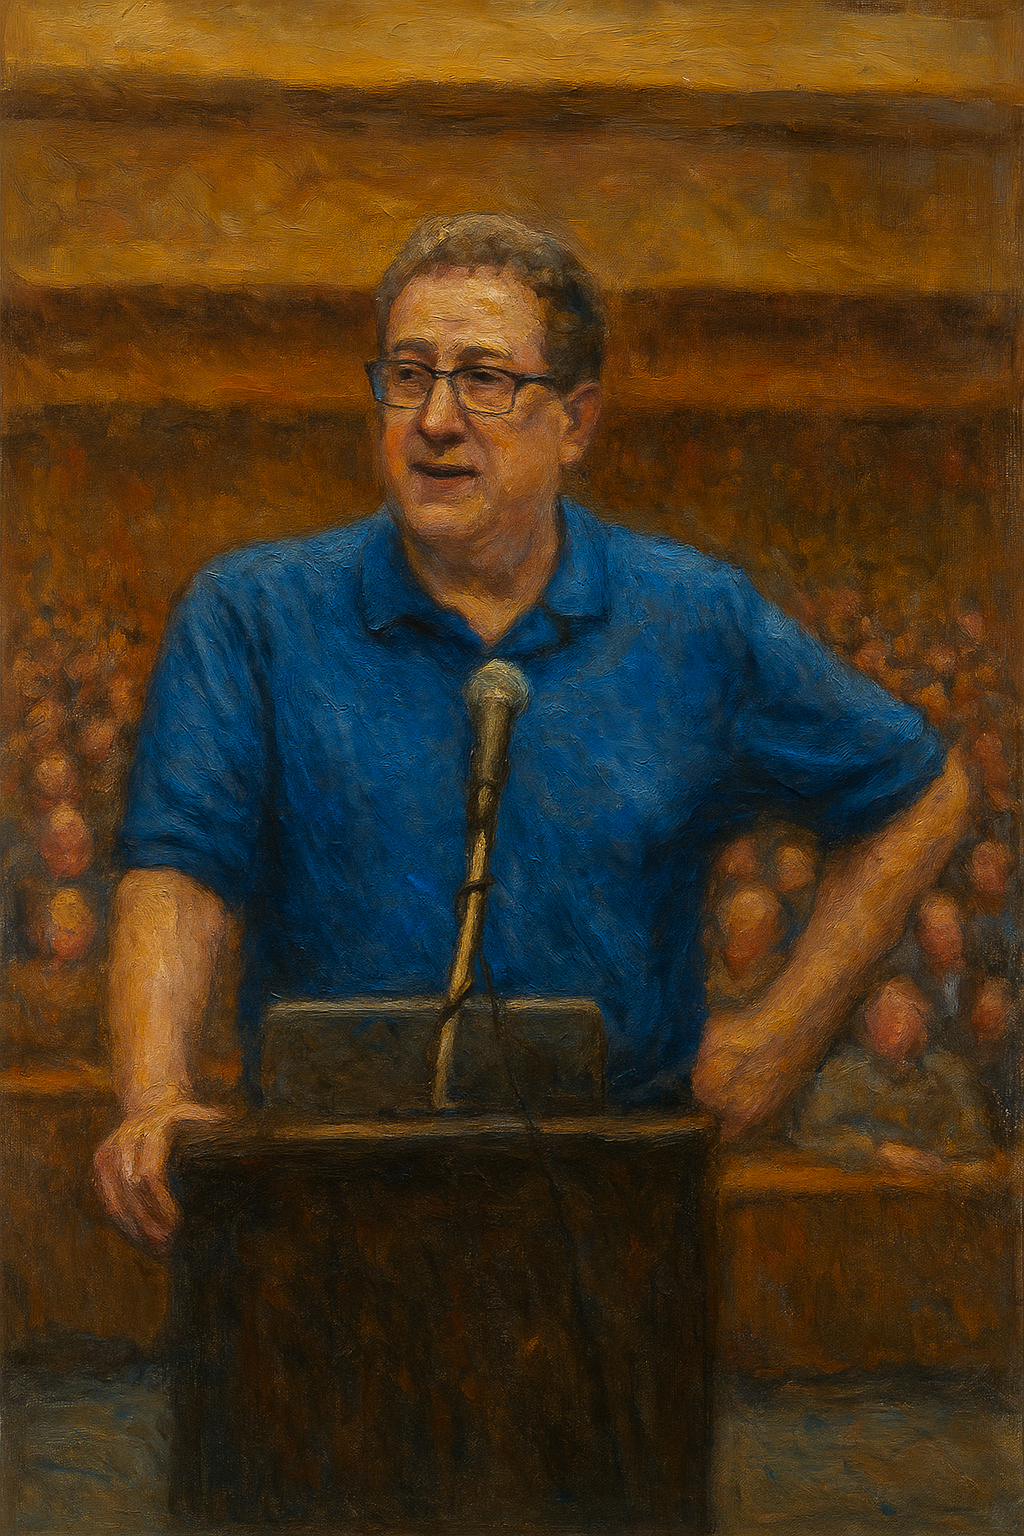
\includegraphics[width=8.5cm]{Abbildungen/david-beazley}
\caption{The creator of Ply, David M.~Beazley.}
\label{fig:david-beazley.png}
\end{figure}


After introducing the concept of regular expressions, we will now explore their practical applications. We
examine the parser generator \texttt{Ply}\index{$\texttt{Ply}$}, which is capable of generating both \textsl{Python}
\emph{scanners} and \textsl{Python} \emph{parsers}.  In this chapter, we will only discuss the generation of
scanners via \texttt{Ply}.
A \textcolor{blue}{scanner}\index{scanner} is a program
designed to segment a given string into a sequence of \emph{tokens}, where a
\textcolor{blue}{token}\index{token} is a contiguous string of characters that logically group together. To
illustrate, consider the input for a \texttt{C}-compiler, which is an \textsc{Ascii}-string representing a
valid \texttt{C} program. The compiler initially organizes these characters into various tokens, including: 

\begin{enumerate}
\item \textcolor{blue}{Keywords} or reserved words, such as, for example, ``\texttt{if}'', ``\texttt{while}'', ``\texttt{for}'', and ``\texttt{switch}''.
\item \textcolor{blue}{Operator symbols}, for example ``\texttt{+}'', ``\texttt{+=}'', ``\texttt{<}'', and ``\texttt{<=}''.
\item \textcolor{blue}{Parentheses}, which include ``\texttt{(}'', ``\texttt{[}'', ``\texttt{\{}'', and their corresponding closing symbols.
\item \textcolor{blue}{Constants}, with \texttt{C} recognizing three types:
    \begin{enumerate}
    \item Numerical constants, such as the integer ``\texttt{42}'' or the floating-point number ``\texttt{1.23e2}''.
    \item String constants enclosed in double quotes, like ``\texttt{\symbol{34}hello\symbol{34}}''.

          Note that the double quote character ``\texttt{\symbol{34}}'' is part of the string constant.
    \item Single-character constants wrapped in single quotes, as in ``\texttt{\symbol{39}a\symbol{39}}''.

          Note that the single quote character ``\texttt{\symbol{39}}'' is part of the character constant.
    \end{enumerate}
\item \textcolor{blue}{Identifiers}, which may serve as variable names, function names, or type names.
\item \textcolor{blue}{Comments}, available in two forms: \textcolor{blue}{Single-line comments} start with
      ``\texttt{//}'' and extend to the end of the line, while \textcolor{blue}{multi-line comments} begin with
      ``\texttt{/*}'' and end with ``\texttt{*/}''. 
\item \textcolor{blue}{Whitespace characters}, such as the \textcolor{blue}{blank character} \texttt{' '}, the \textcolor{blue}{tab} \texttt{'\symbol{92}t'}, the \textcolor{blue}{newline} \texttt{'\symbol{92}n'}, and the \textcolor{blue}{carriage return} \texttt{'\symbol{92}r'}. 

Both whitespace characters and comments are generally discarded by the scanner.
\end{enumerate}

\begin{figure}[!ht]
\centering
\begin{Verbatim}[ frame         = lines, 
                  framesep      = 0.3cm, 
                  firstnumber   = 1,
                  labelposition = bottomline,
                  numbers       = left,
                  numbersep     = -0.2cm,
                  xleftmargin   = 0.8cm,
                  xrightmargin  = 0.8cm,
                ]
    /* Hello World program */
    #include <stdio.h>
    
    int main() {
        printf("Hello World!");
        return 1;
    }
\end{Verbatim}
\vspace*{-0.3cm}
\caption{A straightforward \texttt{C} program.}
\label{fig:hello-world.c}
\end{figure}

\noindent
For a more tangible example, consider Figure \ref{fig:hello-world.c} on page \pageref{fig:hello-world.c}, which
presents a \texttt{C} program that outputs the string ``\texttt{Hello World!}'' along with a newline
character. The scanner processes this program into the subsequent list of tokens:
\pagebreak

\noindent
\hspace*{1.3cm}
   [ ``\texttt{\#}'', ``\texttt{include}'', ``\texttt{<}'', ``\texttt{stdio.h}'', ``\texttt{>}'',
   ``\texttt{int}'', ``\texttt{main}'', ``\texttt{(}'', ``\texttt{)}'', ``\texttt{\{}'',
\\
\hspace*{1.4cm} 
     ``\texttt{printf}'', ``\texttt{(}'', ``\texttt{"Hello World!"}'', ``\texttt{)}'', ``\texttt{;}'', ``\texttt{return}'', ``\texttt{1}'', ``\texttt{;}'', ``\texttt{\}}''
   ]
   \\[0.2cm]
Note that the scanner omits all white space characters, except those that occur inside string constants, as
they are only used to demarcate tokens.  Furthermore, the comment has been removed by the scanner.

While it is feasible to manually create a scanner, using a \textcolor{blue}{scanner generator} makes the task
considerably simpler. We will explore one such utility in the following section. 

\section{The Structure of a \texttt{Ply} Scanner Specification}
In this section, we explore \href{https://www.dabeaz.com/ply/}{Python Lex-Yacc}, \index{ply} commonly known as
\texttt{Ply}. \index{\texttt{Ply}} According to its \href{https://www.dabeaz.com/ply/}{official webpage},
\\[0.2cm]
\hspace*{1.3cm}
``\texttt{Ply} serves as a lex and yacc parsing toolkit for \textsl{Python}.''
\\[0.2cm]
\href{https://en.wikipedia.org/wiki/Lex_(software)}{Lex} is a popular scanner generator for the programming
language \texttt{C}, while \href{https://en.wikipedia.org/wiki/Yacc}{Yacc} is a parser generator for
\texttt{C}.  The toolkit \texttt{Ply} was developed by
\href{https://www.dabeaz.com/}{David Beazley}. In this section, we focus solely on its capabilities as a
scanner generator. In Chapter \ref{chapter:ply} we will discuss how to use \texttt{Ply} as a parser generator. 

To illustrate the core components of a \texttt{Ply} scanner specification, we consider a simple example that
tokenizes arithmetic expressions. This example is adapted from the official \texttt{Ply}
\href{https://ply.readthedocs.io/en/latest/ply.html#specification-of-tokens}{documentation}. A \texttt{Ply}
scanner specification generally consists of three key parts, as demonstrated in Figure
\ref{fig:Ply-Example.ipynb}: 
\begin{enumerate}
\item The module \texttt{ply.lex} contains the definition of the function \texttt{ply.lex.lex()}
      that is able to generate a scanner.
      Therefore, this module is imported in line 1.
\item The first part of a scanner specification is the \blue{token declaration section}.
      Syntactically, this is just a list containing the names of all tokens.  Note that all token names have to
      start with a capital 
      letter.

      In Figure \ref{fig:Ply-Example.ipynb} the token declaration section extends from line 3 to line 11.
\item The second part contains the \blue{token definitions}.  There are two kinds of token definitions:
      \begin{enumerate}
      \item \blue{Immediate token definitions} \index{immediate token definition} have the following form:
            \\[0.2cm]
            \hspace*{1.3cm}
            \texttt{t\_\textsl{NAME} = r'\textsl{regexp}'}
            \\[0.2cm]
            Here \textsl{NAME} has to be one of the names declared in the declaration section and
            \textsl{regexp} is a regular expression using the syntax that is specified in the 
            \textsl{Python} \href{https://docs.python.org/3/library/re.html}{\texttt{re}} module.
      \item \blue{Functional token definitions} \index{functional token definitions} are syntactically
            \textsl{Python function definitions} and have the following form:
            \\[0.2cm]
            \hspace*{1.3cm}
            \texttt{def t\_\textsl{NAME}(t):} \\
            \hspace*{2.05cm}
            \texttt{r'\textsl{regexp}'} \\
            \hspace*{2.8cm} $\vdots$ \\[0.2cm]
            Here, the vertical dots \ ``$\;\vdots\;$'' \ denote any \textsl{Python} code, while
            \textsl{NAME} has to be one of the token names declared in the declaration section and
            \textsl{regexp} is a regular expression.
            
            The functional token definition shown in line 20--23 takes a token \texttt{t} as its
            argument.  This token has the attribute \texttt{t.value}, which refers to the string that has been
            recognized as this token.  In this case, this string is a sequence of digits that can be
            interpreted as a number.  In line 22 the function  \texttt{t\_NUMBER} converts this string into a
            number and stores this number as the attribute \texttt{t.value}.  Finally, the token \texttt{t}
            itself is returned.  This is a typical case where we need a functional token definition since we 
            want to modify the token that is returned.
      \end{enumerate}
      In Figure \ref{fig:Ply-Example.ipynb} the token definitions start in line 13 and end in line 23.
\item The third part deals with the handling of newlines, ignored characters, and scanner errors.
  \begin{enumerate}
  \item A \texttt{Ply} input file may contain the definition of the function \texttt{t\_newline}.
        This function is supposed to deal with newlines contained in the input.  The main purpose of this
        function is to set the  
        counter \texttt{t.lexer.lineno}.  Every token \texttt{t} has the attribute \texttt{t.lexer}, which is a
        reference to the scanner object.  In turn, the scanner object has the attribute \texttt{lineno}, which
        is supposed to be an integer containing the number of the line currently scanned.  This integer starts
        at the value $1$.  Every time a newline is read it should be incremented.

        In line 26 the regular expression \texttt{r'\symbol{92}n+'} matches any positive number of newlines.
        Hence the counter \texttt{lineno} has to be incremented by the length of the string \texttt{t.value.}

        Note that the function \texttt{t\_newline} does \underline{not} return a token.
  \item Line 29 specifies that both blanks and tabs should be ignored by the scanner.
        Note that the string 
        \\[0.2cm]
        \hspace*{1.3cm}
        ``\texttt{' \symbol{92}t'}'' 
        \\[0.2cm]
        is \underline{not} interpreted as a regular expression
        but rather as a list of its characters.  Furthermore, this is not a raw string and must not be prefixed
        with the character ``\texttt{r}'', for otherwise the character sequence ``\texttt{\symbol{92}t}'' would not be
        interpreted as a tab symbol.
  \item The function \texttt{t\_error} deals with characters that can not be recognized.
        An error message is printed and the call \texttt{t.lexer.skip(1)} discards the character that could not be
        matched. 
  \end{enumerate}
\item In line 35 the function \texttt{lex.lex} creates the scanner that has been specified.
\item Line 38 shows how data can be fed into this scanner.
\item In order to use this scanner we can just iterate over it as shown in line 40.  This iteration scans the
      input string using the generated scanner and produces the tokens that are recognized by the scanner one
      by one.  
\end{enumerate}

\begin{figure}[!ht]
\centering
\begin{Verbatim}[ frame         = lines, 
                  framesep      = 0.3cm, 
                  labelposition = bottomline,
                  numbers       = left,
                  numbersep     = -0.2cm,
                  xleftmargin   = 0.8cm,
                  xrightmargin  = 0.8cm,
                ]
    import ply.lex as lex
    
    tokens = [
       'NUMBER',
       'PLUS',
       'MINUS',
       'TIMES',
       'DIVIDE',
       'LPAREN',
       'RPAREN'
    ]
    
    t_PLUS    = r'\+'
    t_MINUS   = r'-'
    t_TIMES   = r'\*'
    t_DIVIDE  = r'/'
    t_LPAREN  = r'\('
    t_RPAREN  = r'\)'
    
    def t_NUMBER(t):
        r'0|[1-9][0-9]*'
        t.value = int(t.value)
        return t
    
    def t_newline(t):
        r'\n+'
        t.lexer.lineno += len(t.value)
    
    t_ignore  = ' \t'
    
    def t_error(t):
        print("Illegal character '%s'" % t.value[0])
        t.lexer.skip(1)
    
    lexer = lex.lex()
    
    data = '3 + 4 * 10 + 007 + (-20) * 2'
    lexer.input(data)
    
    for tok in lexer:
        print(tok)
\end{Verbatim}
\vspace*{-0.3cm}
\caption{A simple scanner Specification for \texttt{Ply}.}
\label{fig:Ply-Example.ipynb}
\end{figure}

\noindent
Executing the program depicted in Figure \ref{fig:Ply-Example.ipynb} yields the following output:

\begin{verbatim}
    LexToken(NUMBER,3,1,0)
    LexToken(PLUS,'+',1,2)
    LexToken(NUMBER,4,1,4)
    % ... (rest of the output)
    LexToken(NUMBER,2,1,27)
\end{verbatim}
The scanner returns tokens as instances of the \texttt{LexToken} class, which possess four distinct attributes:
\begin{enumerate}
\item The \blue{\texttt{type}} attribute indicates the type of the token. It holds a string value that
      corresponds to one of the declared tokens. 
\item The \blue{\texttt{value}} attribute usually contains the recognized string. However, this attribute is
      mutable, allowing for transformations. For instance, the function \texttt{t\_NUMBER} converts this string
      into an integer. 
\item The \blue{\texttt{lineno}} attribute specifies the line number where the token was identified.
\item The \blue{\texttt{lexpos}} attribute serves as a counter, incremented for each character read.
\end{enumerate}

\homeworkEng
Install \texttt{Ply} and verify that the previously presented example operates as expected.
The program \texttt{Ply} can be installed via the following command provided the appropriate \texttt{conda}
environment has already been activated:
\\[0.2cm]
\hspace*{1.3cm}
\texttt{conda install -c conda-forge ply}

\section{The Syntax of Regular Expressions in \textsl{Python}}
In the preceding chapter, we introduced regular expressions using a minimalistic syntax. While this simplicity
is advantageous for the theoretical discussions in the upcoming chapter---where we explore the implementation of
regular expressions via finite state machines---it can be limiting in practical applications. To address this,
the \textsl{Python} module \blue{\textsl{re}} offers various syntactic abbreviations that facilitate the
use of complex regular expressions in a more concise manner. For an in-depth look at these features, I
have authored a brief tutorial at 
\\[0.2cm]
\hspace*{-1.3cm}
\href{https://github.com/karlstroetmann/Formal-Languages/blob/master/Python/Chapter-03/02-Regexp-Tutorial.ipynb}{https://github.com/karlstroetmann/Formal-Languages/blob/master/Python/Chapter-3/02-Regexp-Tutorial.ipynb}
\\[0.2cm]
that focuses on the key aspects of the \texttt{re} module's regular expressions. For an interactive experience,
it is advisable to consult this tutorial directly. 

The web page \href{https://regex101.com}{regex101.com} can be used to test regular expressions for
various programming languages.  Furthermore the web page
\href{https://regexlearn.com/de/learn/regex101}{https://regexlearn.com/de/learn/regex101} provides a free
interactive tutorial for regular expressions.

\section{A Complex Example: Evaluating an Exam}
This sections presents a more complex example that shows some of the power of \texttt{Ply}.  The
task at hand is the evaluation of an exam.  When I mark an exam I create a file that has a format
similar to the example shown in Figure \ref{fig:result.txt}. 

\begin{figure}[!h]
\centering
\begin{Verbatim}[ frame         = lines, 
                  framesep      = 0.3cm, 
                  labelposition = bottomline,
                  numbers       = left,
                  numbersep     = -0.2cm,
                  xleftmargin   = 0.8cm,
                  xrightmargin  = 0.8cm,
                  commandchars  = \\\{\}
                ]
    Class: Algorithms and Complexity
    Group: TINF22AI1
    MaxPoints = 60
   
    Exercise:      1. 2. 3. 4. 5. 6.
    Jim Smith:     9 12 10  6  6  0
    John Slow:     4  4  2  0  -  -
    Susi Sorglos:  9 12 12  9  9  6
\end{Verbatim}
\vspace*{-0.3cm}
\caption{Results of an Exam}
\label{fig:result.txt}
\end{figure}

\begin{enumerate}
\item The first line contains the keyword ``\texttt{Class}'', a colon ``\texttt{:}'', and then the
      name of the lecture. 
\item The second line specifies the group that has taken the exam.
\item The third line specifies the number of points that are necessary to obtain the best mark.
\item The fourth line is empty.
\item The fifth line numbers the exercises.
\item After that, there is a table.  Every row in this table lists the scores achieved by a student
      for each of the exercises.  The name of each student is at the beginning of each row.  The
      name is followed by a colon and after that there is a list of the scores achieved for each
      exercise.  If an exercise has not been attempted at all, the corresponding column contains a hyphen
      ``\texttt{-}''.
\end{enumerate}
I have written a \textsl{Jupyter notebook} that is able to evaluate data of this kind.
You can find the notebook here:
\\[0.2cm]
\hspace*{-1.3cm}
\href{https://github.com/karlstroetmann/Formal-Languages/blob/master/Python/Chapter-03/03-Exam-Evaluation.ipynb}{https://github.com/karlstroetmann/Formal-Languages/blob/master/Python/Chapter-03/03-Exam-Evaluation.ipynb}

\section{Scanner States}
Sometimes, regular expressions are not quite enough and it is beneficial for the scanner to have different
states.  The following example illustrates this.  We will develop a program that is able to convert an 
\textsc{Html} file into a pure text file.  This program is actually quite useful: Some years ago I
had a student who was blind.  If he read a web page, he would use his Braille display.  For him,
the \textsc{Html} markup was of no use so if the markup was removed, he could read web pages faster.
In order to develop the program to remove \textsc{Html} tags, we have to use \blue{scanner states}.
\index{scanner states}  The idea behind scanner states is that the scanner can use different regular
expressions for different parts of the input.  For example, the header of an \textsc{Html} file, i.e.~the part
that is between the \texttt{<head>} and \texttt{</head>} tags, can just be
skipped.  On the other hand, the text inside the \texttt{<body>} and \texttt{</body>} tags needs to be echoed
after any remaining tags have been removed.  The easiest way to achieve this is by using scanner states and
switching between them.  The following notebook shows how this can be done:
\\[0.2cm]
\hspace*{-1.3cm}
\href{https://github.com/karlstroetmann/Formal-Languages/blob/master/Python/Chapter-03/04-Html2Text.ipynb}{https://github.com/karlstroetmann/Formal-Languages/blob/master/Python/Chapter-03/04-Html2Text.ipynb}
\\

\exerciseEng
The purpose of the following exercise is to transform \href{http://www.latex-project.org}{\LaTeX} into 
\href{https://www.tutorialspoint.com/mathml/index.htm}{\textsc{MathML}}.  \LaTeX\ is a document markup language
that is especially well suited to present text that contains mathematical formulas.  In fact, these
lecture notes have all been typeset using \LaTeX.  \textsc{MathML} is the part of \textsc{Html} that
deals with the representation of mathematical formulas.  As \LaTeX\ provides a very rich
document markup language and we can only afford to spend a few hours on this exercise, we confine
ourselves to a small subset of \LaTeX.  Figure \ref{fig:input.tex} on page \pageref{fig:input.tex}
shows the example input file that we want to transform in \textsc{Html}.  If this example file is
typeset using \LaTeX, it is displayed as shown in Figure \ref{fig:input.pdf} on page
\pageref{fig:input.pdf}.  The program that you are
going to develop should transform the \LaTeX\ input file into an \textsc{Html} file.  For your
convenience, all these files are available in the github directory 
\\[0.2cm]
\hspace*{1.3cm}
\href{https://github.com/karlstroetmann/Formal-Languages/tree/master/Python/Chapter-03/05-LaTeX2HTML}{\texttt{Python/LaTeX2HTML}}.
\\[0.2cm]
This directory contains also the \textsl{Jupyter} notebook 
\href{https://github.com/karlstroetmann/Formal-Languages/blob/master/Python/Chapter-03/05-LaTeX2HTML/LaTeX2HTML.ipynb}{\texttt{LaTeX2HTML.ipynb}}.
This notebook contains lots of predefined functions that are useful in order to solve the given task.

\begin{figure}[!ht]
  \centering
\begin{verbatim}
    \documentclass{article}
    \begin{document}
    The sum of the squares of the first $n$ natural numbers is given as:
    $$ \sum\limits_{i=1}^{n} i^{2} = \frac{1}{6} \cdot n \cdot (n+1) \cdot (2\cdot n + 1). $$
    According to Pythagoras, the length of the hypotenuse of a right triangle is
    the square root of the squares of the length of the two catheti:
    $$ c = \sqrt{a^{2} + b^{2}}.  $$
    The area of a circle is given as 
    $$  A = \pi \cdot r^{2},   $$ 
    while its circumference satisfies
    $$ C = 2 \cdot \pi \cdot r.  $$
    \end{document}
    \end{verbatim}
  \caption{An example \LaTeX\ input file.}
  \label{fig:input.tex}
\end{figure}

\begin{figure}[!ht]
  \centering
  \framebox{
  \begin{minipage}{0.8\linewidth}
    The sum of the squares of the first $n$ natural numbers is given as:
    $$ \sum_{i=1}^{n} i^{2} = \frac{1}{6} \cdot n \cdot (n+1) \cdot (2\cdot n + 1). $$
    According to Pythagoras, the length of the hypotenuse of a right triangle is
    the square root of the squares of the length of the two catheti:
    $$ c = \sqrt{a^{2} + b^{2}}.  $$
    The area $A$ of a circle is given as 
    $$  A = \pi \cdot r^{2},   $$ 
    while its circumference satisfies
    $$ C = 2 \cdot \pi \cdot r.  $$   
  \end{minipage}}
  \caption{Output produced by the \LaTeX\ file shown in Figure \ref{fig:input.tex}}
  \label{fig:input.pdf}
\end{figure}

In order to do this exercise, you have to understand a little bit about \LaTeX\ and about 
\textsc{MathML}.  In the following, we discuss those features of these two language that are needed in order to
solve the given problem.
\begin{enumerate}
\item A \LaTeX\ input file has the following structure:
      \begin{enumerate}
      \item The first line list the type of the document.  In our example, it reads
            \\[0.2cm]
            \hspace*{1.3cm}
            \texttt{\symbol{92}documentclass\{article\}}.
            \\[0.2cm]
            This line will be transformed into the following \textsc{Html}:
            \begin{verbatim}
 <html>
 <head>
 <script type="text/javascript"
 src="http://cdn.mathjax.org/mathjax/latest/MathJax.js?config=TeX-AMS-MML_HTMLorMML">
 </script>
 </head>
            \end{verbatim}
            Here, the \texttt{<script>} tag is necessary in order for the \textsc{MathML} 
            to be displayed correctly.
      \item The next line has the form:
            \\[0.2cm]
            \hspace*{1.3cm}
            \texttt{\symbol{92}begin\{document\}}
            \\[0.2cm]
            This line precedes the content and should be translated into the tag
            \\[0.2cm]
            \hspace*{1.3cm}
            \texttt{<body>}.
      \item After that, the \LaTeX\ file consists of text that contains mathematical formula.
      \item The \LaTeX\ input file finishes with a line of the form
            \\[0.2cm]
            \hspace*{1.3cm}
            \texttt{\symbol{92}end\{document\}}.
            \\[0.2cm]
            This line should be translated into the tags
            \\[0.2cm]
            \hspace*{1.3cm}
            \texttt{</body></html>}.
      \end{enumerate}
\item In \LaTeX, an inline formula is started and ended with a single dollar symbol
      ``\texttt{\symbol{36}}''.  
      In \textsc{MathML}, an inline formula is written as
      \\[0.2cm]
      \hspace*{1.3cm}
      \texttt{<math xmlns="http://www.w3.org/1998/Math/MathML" display='inline'>$\cdots$</math>}.
      \\[0.2cm]
      Here, I have used ``$\cdots$'' to represent the mathematical content of the formula.
\item In \LaTeX, a formula that is displayed in its own line is started and ended with the string
      ``\texttt{\symbol{36}\symbol{36}}''.  
      In \textsc{MathML}, these formulas\ are called \blue{block formulas} and are written as
      \\[0.2cm]
      \hspace*{1.3cm}
      \texttt{<math xmlns="http://www.w3.org/1998/Math/MathML" display='block'>$\cdots$</math>}.
      \\[0.2cm]
      Again, I have used ``$\cdots$'' to represent the mathematical content of the formula.
\item While in \LaTeX\ a mathematical variable does not need any special markup, in \textsc{MathMl}
      a mathematical variable is written using the tags 
      \texttt{<mi>} and \texttt{</mi>}.  For example, the mathematical variable $n$ is written as    
      \\[0.2cm]
      \hspace*{1.3cm}
      \texttt{<mi>n</mi>}.
\item While in \LaTeX\ a number does not need any special markup, in \textsc{MathMl}
      a number is written using the tags 
      \texttt{<mn>} and \texttt{</mn>}.  For example, the number $3.14159$ is written as    
      \\[0.2cm]
      \hspace*{1.3cm}
      \texttt{<mn>3.14159</mn>}.
\item In \LaTeX\ the mathematical constant $\pi$ is written using the command ``\texttt{\symbol{92}pi}''.
      In \textsc{MathMl}, we have to make use of the \textsc{Html} entity ``\texttt{\&pi;}'' and
      hence we would write $\pi$ as
      \\[0.2cm]
      \hspace*{1.3cm}
      \texttt{<mn>\&pi;</mn>}.
\item In \LaTeX\ the multiplication operator ``$\cdot$'' is written using the command ``\texttt{\symbol{92}cdot}''.
      In \textsc{MathMl}, we have to make use of the \textsc{Html} entity ``\texttt{\&sdot;}'' and
      hence we would write ``$\cdot$'' as
      \\[0.2cm]
      \hspace*{1.3cm}
      \texttt{<mop>\&sdot;</mop>}.
\item While in \LaTeX\ most operator symbols stand for themselves, in \textsc{MathMl}
      an operator is surrounded by the tags 
      \texttt{<mop>} and \texttt{</mop>}.  For example, the operator $+$ is written as    
      \\[0.2cm]
      \hspace*{1.3cm}
      \texttt{<mop>+</mop>}.
\item In \LaTeX, raising an expression $e$ to the $n$th power is done using the operator
      ``\texttt{\symbol{94}}''.  Furthermore, the exponent should be enclosed in the curly braces
      ``\texttt{\{}'' and ``\texttt{\}}''.  For example, the code to produce the term $x^2$ is
      \\[0.2cm]
      \hspace*{1.3cm}
      \texttt{x\symbol{94}\{2\}}.
      \\[0.2cm]
      In \textsc{MathMl}, raising an expression to a power is achieved using the tags
      \texttt{<msup>} and \texttt{</msup>}.  For example, in order to display the term $x^2$, we
      have to write  
      \\[0.2cm]
      \hspace*{1.3cm}
      \texttt{<msup><mi>x</mi><mn>2</mn></msup>}.
\item In \LaTeX, taking the square root of an expression is done using the command
      ``\texttt{\symbol{92}sqrt}''.  The argument has to be enclosed in curly braces.
      For example, in order to produce the output $\sqrt{a+b}$, we have to write
      \\[0.2cm]
      \hspace*{1.3cm}
      \texttt{\symbol{92}sqrt\{a+b\}}.
      \\[0.2cm]
      In \textsc{MathMl}, taking the square root makes use of the tags \texttt{<msqrt>} 
      and \texttt{</msqrt>}.  The example shown above can be written as
      \\[0.2cm]
      \hspace*{1.3cm}
      \texttt{<msqrt><mi>a</mi><mop>+</mop><mi>b</mi></msqrt>}.
\item In \LaTeX, writing a fraction is done using the command
      ``\texttt{\symbol{92}frac}''.  This command takes two arguments, the numerator and the
      denominator.  Both of these have to be enclosed in curly braces.
      For example, in order to produce the output $\frac{a+b}{2}$, we have to write
      \\[0.2cm]
      \hspace*{1.3cm}
      \texttt{\symbol{92}frac\{a+b\}\{2\}}.
      \\[0.2cm]
      In \textsc{MathMl}, a fraction is created via the tags \texttt{<mfrac>} 
      and \texttt{</mfrac>}.  Additionally, if the arguments contain more than a single element,
      each of them has to be enclosed in the tags \texttt{<mrow>} and \texttt{</mrow>}.
      The example shown above can be written as
      \\[0.2cm]
      \hspace*{1.3cm}
      \texttt{<mfrac><mrow><mi>a</mi><mop>+</mop><mi>b</mi></mrow><mn>2</mn></mfrac>}.
\item In \LaTeX, writing a sum is done using the command
      ``\texttt{\symbol{92}sum\symbol{92}limits}''.  
      This command takes two arguments:  The first argument gives the indexing variable together
      with its lower bound, while the second argument gives the upper bound.  The first argument
      is started using the string ``\texttt{\_\{}'' and ended using the string ``\texttt{\}}'',
      while the second argument is started using the string ``\texttt{\symbol{94}\{}'' and ended using the
      string ``\texttt{\}}''.  For example, in order to produce the output 
      \\[0.2cm]
      \hspace*{1.3cm}
      $\displaystyle\sum\limits_{i=1}^{n} i$,
      \\[0.2cm]
      we have to write
      \\[0.2cm]
      \hspace*{1.3cm}
      \texttt{\symbol{92}sum\symbol{92}limits\_\{i=1\}\symbol{94}\{n\} i}.
      \\[0.2cm]
      In \textsc{MathMl}, a sum with lower and upper limits is created via the tags
      \texttt{<munderover>} and \texttt{</munderover>} and the \textsc{Html} entity ``\texttt{\&sum}''.
      The tag \texttt{munderover} takes three arguments:
      \begin{enumerate}
      \item The first argument is the operator, so in this case it is the entity ``\texttt{\&sum}''.
      \item The second argument initializes the indexing variable of the sum.
      \item The third argument provides the upper bound.
      \end{enumerate}
      The second argument usually contains more than a single item and therefore has to be enclosed 
      in the tags \texttt{<mrow>} and \texttt{</mrow>}.
      Hence, the example shown above would be written as follows:
      
    \begin{verbatim}
    <munderover>
        <mo>&sum;</mo>
        <mrow>
            <mi>i</mi> <mo>=</mo> <mn>1</mn>
        </mrow>
        <mi>n</mi>
    </munderover>
    \end{verbatim}
\end{enumerate}

\remarkEng
The most important problem that you have to solve is the following:  Once you encounter a closing brace
``\texttt{\}}'' you have to know whether this brace closes the argument of a square root, a
fraction, a sum, or an exponent.  You should be aware that, for example, square roots and fractions
can be nested.  Hence, it is not enough to have a single variable that remembers whether you are
parsing, say, a square root or a fraction.  Instead, every time you encounter a string like, e.g.
\\[0.2cm]
\hspace*{1.3cm}
\texttt{\symbol{92}sqrt\{} \quad or \quad \texttt{\symbol{92}frac\{},
\\[0.2cm]
you should store the current state on a stack and set the new state according to whether you have just seen the
keyword ``\texttt{\symbol{92}frac}'' or ``\texttt{\symbol{92}sqrt}'' or whatever caused the
curly brace to be opened.  When you encounter a closing brace ``\texttt{\}}'', you should 
restore the state to its previous value by looking up this value from the stack.  
\eox

\section{Check your Understanding}
\begin{enumerate}[(a)]
\item How are regular expressions defined in \textsl{Python}?
\item Do you understand the structure of a \texttt{Ply} scanner specification?
\item Are you able to use \texttt{Ply} to write a program that reads a given text, finds all numbers inside
      this text that are followed by a $\texttt{\$}$ symbol and that then converts these numbers to their equivalent
      value in \texttt{\euro{}}?  Assume that $1 \mathtt{\$} = 0.85 \texttt{\euro{}}$.
\end{enumerate}



%%% Local Variables: 
%%% mode: latex
%%% TeX-master: "formal-languages.tex"
%%% End: 

\chapter{Finite Automatons \label{chapter:finite-state-machines}} 

\begin{figure}[h] 
\centering
  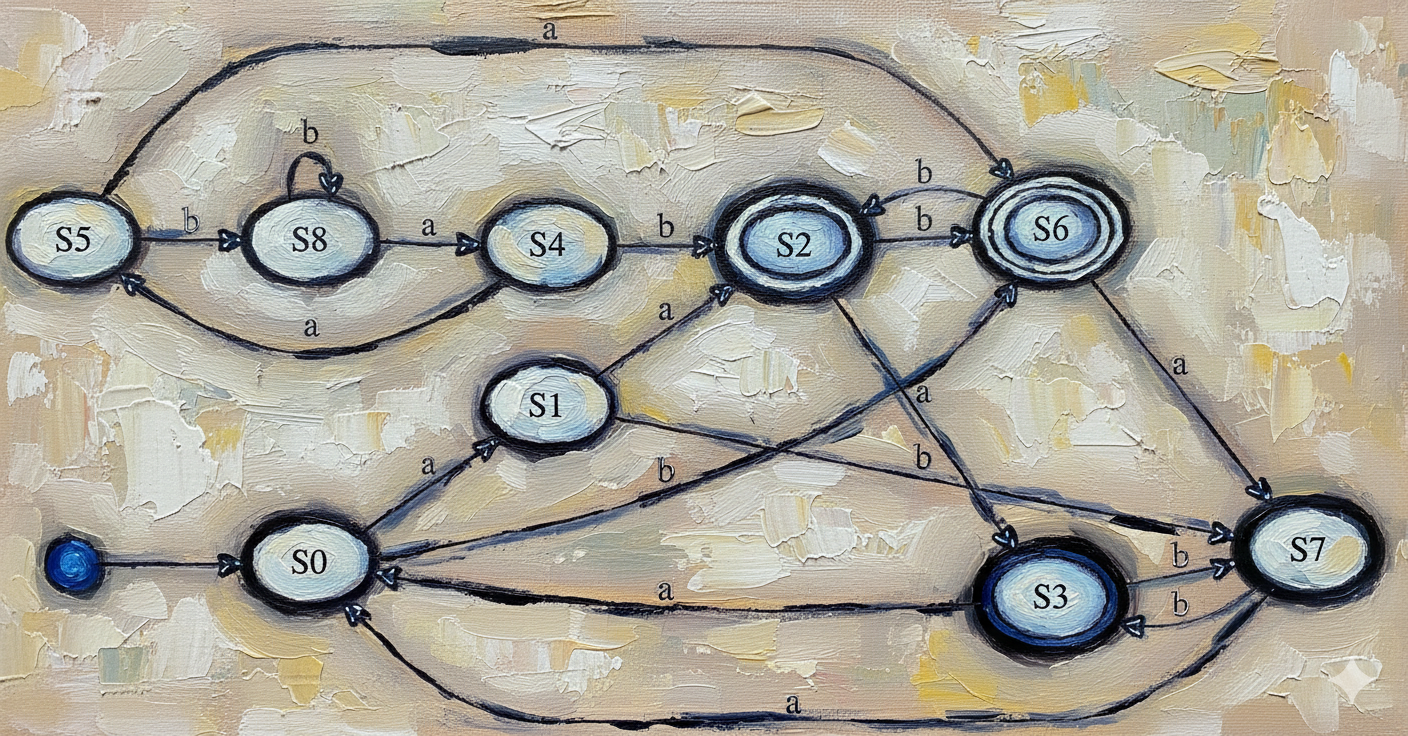
\includegraphics[width=12.5cm]{Abbildungen/finite-state-machine.png}
\caption{A finite state machine.}
\label{fig:finite-state-machine.png}
\end{figure}

\noindent
In the previous chapter we have seen how we can generate scanners from regular expressions.  In this chapter
we learn how regular expressions can be implemented using \blue{finite state automatons},
abbreviated as \textsc{FSA}s. There are two kinds of \textsc{FSA}s: The \blue{deterministic} ones known as
\blue{deterministic finite automatons}, abbreviated as \textsc{DFA} 
and the non-deterministic ones known as \blue{non-deterministic finite automaton}, abbreviated as
\textsc{NFA}s.  Although \textsc{NFA}s seem to be more powerful than \textsc{DFA}s, we will see that every
\textsc{NFA} can be transformed into an equivalent \textsc{DFA}.  After proving this result, we show how a regular
expression can be translated into an equivalent  \textsc{NFA}.  Finally, we show that the
language recognized by any \textsc{DFA} can be described by an equivalent regular expression.  Therefore, the
central result of this chapter is the equivalence of \textsl{FA}s and regular expressions.
In detail, the results proved in this chapter are as follows:
\begin{enumerate}[(a)]
\item The language described by a regular expression can be defined by a \textsc{NFA}.
\item Every \textsc{NFA} can be transformed into an equivalent \textsc{DFA}.
\item For every \textsc{DFA} there is an regular expression specifying the language recognized by
      this \textsc{DFA}.
\end{enumerate}


\section{Deterministic Finite Automatons}
The finite state automatons that we are going to discuss in this chapter are used to read a string and
to decide whether this string is an element of a given language.  Hence, the input of these 
\textsc{DFA}s is a string, while the output is either the value \texttt{True} or the value \texttt{False}.
The name giving feature of an \textsc{DFA} is the fact that an \textsc{DFA} only has a
\underline{finite} number of possible states.  Reading a character causes the \textsc{DFA} to change its state.
A \textsc{DFA} accepts its input if it has reached a so called \blue{accepting state} after reading
all characters of the input string.  Let me explain this idea more precisely:
\begin{enumerate}[(a)]
\item Initially, the \textsc{DFA} is in a state that is known as the \blue{start state}. \index{start state}
\item In every step of its computation, the \textsc{DFA} reads one character of the input string
      $s$.  Every time a character is processed, the state of the \textsc{DFA} might change.
\item Some states of the \textsc{DFA} are designated as \blue{accepting states}.  \index{accepting state}
      If the \textsc{DFA} has consumed all characters of the given input string $s$ and the \textsc{DFA}
      has reached an accepting state, then the input string $s$ is accepted and the \textsc{DFA}
      returns \texttt{True}.  Otherwise the \textsc{DFA} returns \texttt{False} and the string $s$
      is rejected.
\end{enumerate}
\begin{figure}[!ht]
  \centering
      \epsfig{file=Abbildungen/abstara.eps, scale=0.7}
   \caption{A \textsc{DFA} to recognize the language $L(\texttt{a}^*\cdot\texttt{b}\cdot\texttt{a}^*)$.}
  \label{fig:abstara.dot}
\end{figure}


\noindent
Finite state automatons are best presented graphically.  Figure \ref{fig:abstara.dot} depicts a simple
\textsc{DFA} that recognizes those strings that are specified by the regular expression
\\[0.2cm]
\hspace*{1.3cm}
$\texttt{a}^*\cdot\texttt{b}\cdot\texttt{a}^*$.
\\[0.2cm]
This \textsc{DFA} has but two states.  These states are called $0$ and $1$.
\begin{enumerate}
\item State $0$  is the start state.  In Figure \ref{fig:abstara.dot}, the start state is indicated by an arrow
      coming from the left that points to it.  
  
      If the \textsc{DFA} is in the state $0$ and reads the character ``\texttt{a}'', then the
      \textsc{DFA} stays in the state $0$.  This is specified in the figure by an arrow labeled with the
      character ``\texttt{a}'' that both starts and ends in the state $0$.  On the other hand, if the
      character ``\texttt{b}'' is read while the \textsc{DFA} is in state 0, then the \textsc{DFA}
      switches into the state $1$.  This is depicted by an arrow labeled with the character
      ``\texttt{b}'' that originates from the state $0$ and points to the state $1$.
\item State  $1$ is an accepting state. In Figure \ref{fig:abstara.dot} this is specified by the
      fact that the state $1$ is decorated by a double circle.

      If the character ``\texttt{a}'' is read while the \textsc{DFA} is in state $1$, then the
      \textsc{DFA} does not change its state.  On the other hand, if the \textsc{DFA} reads the
      character ``\texttt{b}'' while in state $1$, then the next state is undefined since there is no
      arrow originating from state $1$ that is labeled with the character ``\texttt{b}''.

      In general, a \textsc{DFA} \blue{dies} \index{death of a \textsc{DFA}}
      if it reads a character $c$ in a state $s$ such that there is no transition from $s$ when $c$ is read.
      In this case, the \textsc{DFA} does not accept the given input string.
\end{enumerate}

\noindent
Formally, a \href{http://en.wikipedia.org/wiki/Finite-state_machine}{\emph{deterministic finite automaton}} 
\index{deterministic finite automaton}
is defined as a 5-tuple.
\begin{Definition}[\textsc{DFA}]
A \blue{deterministic finite automaton} (abbreviated as \textsc{DFA}\index{\textsc{DFA}}) is a 5-tuple 
\\[0.2cm]
\hspace*{1.3cm}
$F = \langle Q, \Sigma, \delta, q_0, A\rangle$
\\[0.2cm]
where the components $Q$, $\Sigma$, $\delta$, $q_0$, and $A$ have the following properties:
\begin{enumerate}
\item $Q$ is the \underline{finite} \blue{set of states}.
\item $\Sigma$ is the \blue{input alphabet}\index{input alphabet}\index{$\Sigma$}.  Therefore, $\Sigma$ is a
      set of characters and 
      the strings read by the \textsc{DFA} $F$ are strings from the set $\Sigma^*$.
\item $\delta: Q \times \Sigma \rightarrow Q \cup \{ \Omega \}$

      is the  \blue{transition function}\index{transition function}.  For every state $q\in Q$ and for all
      characters $c \in \Sigma$ the expression $\delta(q,c)$ computes the new state of the \textsc{DFA} $F$
      that is reached if $F$ reads the character $c$ while in state $q$.
      If $\delta(q,c) = \Omega$, then $F$ \blue{dies} when it is in state $q$ and the next character
      is $c$. 

      In the figures depicting \textsc{DFA}s transitions of the form $\delta(q, c) = \Omega$ 
      are not shown.
\item $q_0 \in Q$ is the \blue{start state}. \index{start state}
\item $A \subseteq Q$ is the set of \blue{accepting states}. \index{accepting states, set of}
      \qed
\end{enumerate}
\end{Definition}

\exampleEng
The \textsc{DFA} that is shown in Figure  \ref{fig:abstara.dot} is formally defined as follows:
\\[0.2cm]
\hspace*{1.3cm}
$F = \langle Q, \Sigma, \delta, q_0, A \rangle$,
\\[0.2cm]
where we have:
\begin{enumerate}
\item $Q = \{ 0, 1 \}$,
\item $\Sigma = \{ \texttt{a}, \texttt{b} \}$,
\item $\delta = \bigl\{ 
                        \pair(0,a) \mapsto 0, 
                        \pair(0,b) \mapsto 1, 
                        \pair(1,a) \mapsto 1, 
                        \pair(1,b) \mapsto \Omega 
                \bigr\}$,
\item $q_0 = 0$,
\item $A = \{ 1 \}$.
\end{enumerate}
In order to formally define the language $L(F)$ that is accepted by a \textsc{DFA} $F$
we generalize the transition function $\delta$ to a new function
\\[0.2cm]
\hspace*{1.3cm}
$\delta^*: Q \times \Sigma^* \rightarrow Q \cup \{ \Omega \}$
\\[0.2cm]
that, instead of a single character, accepts a string as its second argument.  The definition of
$\delta^*(q, w)$ is given by induction on the string $w$.
\begin{enumerate}
\item[I.A.] $w = \lambda$:  We define
            \\[0.2cm]
            \hspace*{1.3cm}
            $\delta^*(q, \lambda) := q$,
            \\[0.2cm]
            because if a deterministic \textsc{DFA} does not read any character, it cannot change its state. 
\item[I.S.] $w = cv$ where $c \in \Sigma$ and $v  \in \Sigma^*$:  We define
            \\[0.2cm]
            \hspace*{1.3cm}
            $\delta^*(q, cv) := \left\{
            \begin{array}[c]{ll}              
            \delta^*\bigl(\delta(q,c),v\bigr) & \mbox{provided $\delta(q,c) \not= \Omega$;} \\
            \Omega                            & \mbox{otherwise}.
            \end{array}
            \right.
            $
            \\[0.2cm]
            If $F$ reads the string  $cv$, it first reads the character $c$.  Now if this causes  $F$
            to change into the state $\delta(q,c)$, then $F$ has to read the string $v$ in the state
            $\delta(q,c)$.  However, 
            if  $\delta(q,c)$ is undefined, then  $\delta^*(q,cv)$ is undefined too.
\end{enumerate}

\begin{Definition}[Accepted Language, $L(F)$]
  \index{accepted language} \index{$L(F)$}
  For a \textsc{DFA} $F = \langle Q, \Sigma, \delta, q_0, A \rangle$ the \blue{language accepted by $F$} 
  is called $L(F)$ and is defined as
  \\[0.2cm]
  \hspace*{1.3cm}
  $L(F) := \bigl\{ s \in \Sigma^* \mid \delta^*(q_0,s) \in A \bigr\}$. 
  \\[0.2cm]
  Hence, the accepted language of $F$ is the set of all those strings that take $F$ from its
  start state into an accepting state. \eox
\end{Definition}

\exerciseEng
Specify a \textsc{DFA} $F$ such that $L(F)$ is the set of all those strings $s \in \{a,b\}^*$, 
such that $s$ contains the substring  ``\texttt{aba}''.
\eox


\paragraph{Complete Finite State Machines}
Occasionally it is beneficial for a \textsc{DFA} $F$ to be \blue{complete}: A \textsc{DFA}
\\[0.2cm]
\hspace*{1.3cm}
$F = \langle Q, \Sigma, \delta, q_0, A \rangle$,
\\[0.2cm]
is \blue{complete}\index{complete, finite state machine} if the transition function $\delta$ never returns the
undefined value $\Omega$, i.e.~we have 
\\[0.2cm]
\hspace*{1.3cm}
$\delta(q, c) \not= \Omega$ \quad for all $q \in Q$ and $c \in \Sigma$.

\begin{Proposition}
  For every \textsc{DFA} $F$ there exists a complete \textsc{DFA}  $\widehat{F}$ that accepts
  the same language as the \textsc{DFA}  $F$, i.e.~we have:
  \\[0.2cm]
  \hspace*{1.3cm}
  $L(\widehat{F}) = L(F)$.
\end{Proposition}

\proofEng
Assume $F$ is given as
\\[0.2cm]
\hspace*{1.3cm}
$F = \langle Q, \Sigma, \delta, q_0, A \rangle$.
\\[0.2cm]
The idea is to define $\widehat{F}$ by adding a new state to the set of states $Q$.  This new state is called
the  \blue{dead state}. \index{dead state} If there is no next state for a given state  $q \in Q$ when a character $c$
is processed, i.e.~if we have
\\[0.2cm]
\hspace*{1.3cm}
$\delta(q, c) = \Omega$,
\\[0.2cm]
then $F$ changes into the dead state.  Once $F$ has reached a dead state, it will never leave this
state.

The formal definition of the \textsc{DFA} $\widehat{F}$ is done as follows:
We introduce a new state $\skull$ which serves as the \blue{dead state}.  The only requirement is that $\skull \not\in Q$.
\begin{enumerate}
\item $\widehat{Q} := Q \cup \{ \skull \}$,

      the dead state is added to the set  $Q$.
\item $\widehat{\delta} : \widehat{Q} \times \Sigma \rightarrow \widehat{Q}$,

      where the function $\widehat{\delta}$ is defined as follows:
      \begin{enumerate}
      \item $\delta(q,c) \not= \Omega \rightarrow \widehat{\delta}(q,c) = \delta(q,c)$ \quad  for all $q \in Q$ and $c \in \Sigma$.

            If the state transition function is defined for the state  $q$ and the character
            $c$, then $\widehat{\delta}(q,c)$ is the same as $\delta(q,c)$.
      \item $\delta(q,c) = \Omega \rightarrow \widehat{\delta}(q,c) = \skull$  \quad for all $q \in Q$ and $c \in \Sigma$.

            If the state transition function $\delta$ is undefined for the state $q$ and the character
            $c$, then $\widehat{\delta}(q,c)$ returns the dead state $\skull$.
      \item $\widehat{\delta}(\skull, c) = \skull$ \quad for all $c \in \Sigma$,

            because there is no escape from death.
      \end{enumerate}
\end{enumerate}
Hence the \textsc{DFA}  $\widehat{F}$ is given as follows:
\\[0.2cm]
\hspace*{1.3cm}
$\widehat{F} = \langle \widehat{Q}, \Sigma, \widehat{\delta}, q_0, A \rangle$.
\\[0.2cm]
If  $F$ reads a string $s$ without reaching an undefined state, then the behavior of $F$ and $\widehat{F}$ is the same.
However, if $F$ reaches an undefined state, then $\widehat{F}$ instead switches into the dead state 
$\skull$ and remains in this state regardless of the rest of the input string.  As the dead state $\skull$
is not an accepting state, the languages accepted by  $F$ and $\widehat{F}$ are identical. \qed 

\exerciseEng
Define a \textsc{DFA} that accepts the language specified by the regular expression 
\\[0.2cm]
\hspace*{1.3cm}
$r := (\texttt{a}+\texttt{b})^* \cdot \texttt{b} \cdot (\texttt{a}+\texttt{b}) \cdot
(\texttt{a}+\texttt{b})$. \eox

\solutionEng
The regular expression $r$ specifies those strings $s$ from the alphabet 
$\Sigma = \{ \mathtt{a}, \mathtt{b} \}$ such that the antepenultimate character of $s$ is the
character ``\texttt{b}''.  In order to recognize this fact, the \textsc{DFA} has to remember the
last three characters.  As there are eight different possible combinations for the last three
characters, the \textsc{DFA} needs to have eight states.  Let us number these states 
 $0$, $1$, $2$, $\cdots$, $7$.  We describe the purpose of these states in the following:
\begin{description}
\item[State 0:] In this state, the character ``\texttt{b}'' has not yet been seen. 
  Depending on how many characters have been read, there are four cases:
  \begin{enumerate}[(a)]
  \item At least three characters have been read.  In this case, the last three characters are ``\texttt{aaa}''.  
  \item Two characters have been read.  In this case, the string that has been read so far is the string ``\texttt{aa}''.  
  \item Only one character has been read so far. In this case, the string that has been read is ``\texttt{a}''.  
  \item Nothing has yet been read and therefore the string that has been read is $\lambda$.
  \end{enumerate}

                For the remaining states we list the last three characters  that have been read
                without further comment.
\item[State 1:] ``\texttt{aab}''.

                This case also covers the cases where the strings ``\texttt{ab}'' and ``\texttt{b}''
                have been read.
\item[State 2:] ``\texttt{aba}''.

                This case also cover the case where the string ``\texttt{ba}'' 
                has been read.
\item[State 3:] ``\texttt{abb}''.

                This case also cover the case where the string ``\texttt{bb}'' 
                has been read.
\item[State 4:] ``\texttt{bab}''.
\item[State 5:] ``\texttt{bba}''.
\item[State 6:] ``\texttt{bbb}''.
\item[State 7:] ``\texttt{baa}''.
\end{description}
Obviously, the states 4, 5, 6 and 7 are the accepting states because here the antepenultimate
character is the character ``\texttt{b}''.  Next, we construct the transition function $\delta$.
\begin{enumerate}
\item[0.] First, let us consider the state 0.  If the last three characters that have been read are
          ``\texttt{aaa}'' and if we read the character ``\texttt{a}'' next, then the last three
          characters read will again be ``\texttt{aaa}''.  Hence, we must have
          \\[0.2cm]
          \hspace*{1.3cm}
          $\delta(0, \mathtt{a}) = 0$.
          \\[0.2cm]
          However, if instead we read the character ``\texttt{b}'' in state 0, then the last three
          characters that have been read are ``\texttt{aab}'', which is exactly the last three
          characters that have been read in state 1.  Hence we have
          \\[0.2cm]
          \hspace*{1.3cm}
          $\delta(0, \mathtt{b}) = 1$.
\item[1.] Next we consider state 1.  If the last three characters are ``\texttt{aab}'' and we read
          the character ``\texttt{a}'' next, then the last three characters are ``\texttt{aba}''.
          This corresponds to the state  2.  Therefore, we must have
          \\[0.2cm]
          \hspace*{1.3cm}
          $\delta(1, \mathtt{a}) = 2$.
          \\[0.2cm]
          If instead we read the character  ``\texttt{b}'' while in state 1, then the last three
          characters will be ``\texttt{abb}'', which corresponds to the state number  3.  Hence we have
          \\[0.2cm]
          \hspace*{1.3cm}
          $\delta(1, \mathtt{b}) = 3$.
\end{enumerate}
The remaining transitions are found in a similar way.
Figure \ref{fig:abstarbabab.dot} on page \pageref{fig:abstarbabab.dot} shows the resulting \textsc{DFA}.
We still have to explain how we have chosen the start state.  When the computation starts, the
finite state machine has not read any character.  In particular, this implies that neither of the
last three characters is the character ``\texttt{b}''.   Hence we can use the state 0 as the start
state of our \textsc{DFA}.

 \begin{figure}[!ht]
   \centering
       \epsfig{file=Abbildungen/abstarbabab.eps, scale=1.0}
    \caption{A \textsc{DFA} accepting
             $L\bigl((\texttt{a}+\texttt{b})^* \cdot \texttt{b} \cdot (\texttt{a}+\texttt{b}) \cdot (\texttt{a}+\texttt{b})\bigr)$.}
   \label{fig:abstarbabab.dot}
 \end{figure}

\remarkEng
There is a nice tool available that can be used to better understand finite state machines.  This
tool is available at
\\[0.2cm]
\hspace*{1.3cm}
\href{https://ivanzuzak.info/noam/webapps/fsm_simulator/}{\texttt{https://ivanzuzak.info/noam/webapps/fsm\_simulator/}}.


\section{Non-Deterministic Finite Automatons}
For many applications, the \textsc{DFA}s introduced in the previous section are unwieldy
because they have a large numbers of states.  For example, the regular expression to recognize the language
\\[0.2cm]
\hspace*{1.3cm}
$L\bigl((\texttt{a}+\texttt{b})^* \cdot \texttt{b} \cdot (\texttt{a}+\texttt{b}) \cdot (\texttt{a}+\texttt{b})\bigr)$ 
\\[0.2cm]
needs 8 different states since the \textsc{DFA} needs to remember the last three characters that
have been read and there are $2^3 = 8$ combinations of these characters.  
It would be possible to simplify this finite state automaton if the automaton would be permitted to \emph{choose} its
next state from a given set of states.

\begin{figure}[!ht]
  \centering
      \epsfig{file=Abbildungen/abstarbabab-nd.eps, scale=0.7}
   \caption{A non-deterministic finite automaton to recognize 
           $L\bigl((\texttt{a}+\texttt{b})^* \cdot \texttt{b} \cdot (\texttt{a}+\texttt{b}) \cdot (\texttt{a}+\texttt{b})\bigr)$.}
  \label{fig:abstarbabab-nd.dot}
\end{figure}
\noindent
Figure \ref{fig:abstarbabab-nd.dot} presents a \blue{non-deterministic finite automaton} (abbreviated as
\textsc{NFA}) that accepts
the language specified by the regular expression
\\[0.2cm]
\hspace*{1.3cm}
$(\texttt{a}+\texttt{b})^* \cdot \texttt{b} \cdot (\texttt{a}+\texttt{b}) \cdot (\texttt{a}+\texttt{b})$.
\\[0.2cm]
This finite automaton has only 4 different states that are named $0$, $1$, $2$ and $3$.
\begin{enumerate}
\item $0$ is the start state.  If the \textsc{NFA} reads the letter \texttt{a} while it is in this
      state, the \textsc{NFA} will stay in state $0$.  However, if the \textsc{NFA} reads the
      character \texttt{b}, then the finite state automaton has a \emph{choice}:  It can either stay in state
      $0$, or it might switch to the state $1$.
\item In state $1$ the finite state automaton switches to state $2$ if it reads either the character
      \texttt{a} or the character \texttt{b}.
\item In state $2$ the \textsc{NFA} switches to state $3$ if it reads either the character
      \texttt{a} or the character \texttt{b}.
\item State  $3$ is the accepting state.  There is no transition from this state.  Hence, if the
      \textsc{NFA} is in state 3 and there are still characters to read, then the \textsc{NFA} dies.
\end{enumerate}
The finite state automaton in Figure \ref{fig:abstarbabab-nd.dot} is non-deterministic because it has
to guess the next state if it is in state $0$ and reads the character ``\texttt{b}''.  Let us consider a possible
\emph{computation} of the \textsc{NFA} when it reads the input ``\texttt{abab}'':
\\[0.2cm]
\hspace*{1.3cm}
$0 \comp{a} 0 \comp{b} 1 \comp{a} 2 \comp{b} 3$
\\[0.2cm]
In this computation, the \textsc{NFA} has chosen the correct transition when reading the first
occurrence of the character ``\texttt{b}''.  If the \textsc{NFA} had stayed in the state $0$ instead
of switching into the state 1, it would have been impossible to reach the accepting state 3 later
because then the computation would have worked out as follows:
\\[0.2cm]
\hspace*{1.3cm}
$0 \comp{a} 0 \comp{b} 0 \comp{a} 0 \comp{b} 1$
\\[0.2cm] 
Here, the \textsc{NFA} is in state 1 after consuming the input string ``\texttt{abab}'' and as state
1 is not an accepting state, the \textsc{NFA} would have falsely rejected the string ``\texttt{abab}''.
Let us consider a different example where the input is the string ``\texttt{bbbbb}'':
\\[0.2cm]
\hspace*{1.3cm}
$0 \comp{b} 0 \comp{b} 1 \comp{b} 2 \comp{b} 3 \comp{b} \Omega$
\\[0.2cm]
Here, the \textsc{NFA} has switched to early into the state 1.  In this case, the \textsc{NFA} dies
when reading the last character ``\texttt{b}''.  If the \textsc{NFA} had stayed in state $0$ when reading the second
occurrence of the character ``\texttt{b}'', then it would have correctly accepted the string
``\texttt{bbbbb}'' since then the computation could have been as follows:
\\[0.2cm]
\hspace*{1.3cm}
$0 \comp{b} 0 \comp{b} 0 \comp{b} 1 \comp{b} 2 \comp{b} 3$.
\\[0.2cm]
The previous examples show that in order to avoid premature death, the given non-deterministic \textsc{NFA} has
to choose its successor state
\href{https://www.youtube.com/watch?v=c3RN9zz77Cs}{wisely}.  
If $F$ is a non-deterministic \textsc{NFA} and $s$ is a string such that $F$ can, when reading $s$,
choose its successor so that it reaches an accepting state after having read $s$, then the string
$s$ is an element of the language $L(F)$.

It seems that the concept of an \textsc{NFA} is far more powerful than the 
concept of a \textsc{DFA}.  After all, a \textsc{NFA} appears to have some form of clairvoyance for else it
could not guess which states to choose.  However, we will prove in the 
next section that both \textsl{DFA}s and \textsc{NFA}s have the same power to
recognize languages:  Every language recognized by an \textsc{NFA} is also
recognized by a \textsc{DFA}.  In order to prove this claim, we have to
formalize the notion of an \textsc{NFA}.  The definition that follows is more
general than the informal description of an \textsc{NFA}s given so far, as we will
allow the \textsc{NFA} to also have \blue{$\varepsilon$-transitions}\index{$\varepsilon$-transition}.  An $\varepsilon$ transition
allows the \textsc{NFA} to switch its state without reading any character.  For example, if there is
an $\varepsilon$-transition from the state 1 into the state 2, we write
\\[0.2cm]
\hspace*{1.3cm}
$1 \comp{\varepsilon} 2$.


\begin{Definition}[NFA]
A \blue{non-deterministic finite automaton} \index{\textsc{NFA}}
(abbreviated as \blue{\textsc{NFA}}\index{NFA}) 
is a  5-tupel  
\\[0.2cm]
\hspace*{1.3cm}
$\langle Q, \Sigma, \delta, q_0, A\rangle$,
\\[0.2cm]
such that the following holds:
\begin{enumerate}
\item $Q$ is the finite \blue{set of states}.
\item $\Sigma$ is the \blue{input alphabet}.
\item $\delta$ is a function from $Q \times (\Sigma \cup \{ \varepsilon \})$ that assigns a set of states
      $\delta(q, a) \subseteq Q$ to every pair $\pair(q, a)$ from $Q \times (\Sigma \cup \{ \varepsilon \})$:
      \\[0.2cm]
      \hspace*{1.3cm}
      $\delta: Q \times (\Sigma \cup \{\varepsilon\}) \rightarrow 2^Q$.
      \\[0.2cm]
      If $a \in \Sigma$, then $\delta(q, a)$ is the set of states the \textsc{NFA} can switch to
      after reading the character $a$ in state $q$.  The set $\delta\bigl(q, \varepsilon)$ is the
      set of states that can be reached from the state $q$ without reading a character.
      
      As in the deterministic case, $\delta$ is called the \blue{transition function}.
\item $q_0 \in Q$ is the start state.
\item $A \subseteq Q$ is the set of accepting states. 
\end{enumerate}
If we have $q_2 \in \delta(q_1, \varepsilon)$, then the \textsc{NFA} has an
\blue{$\varepsilon$-transition} from the state $q_1$ into the state $q_2$.  This is written as
\\[0.2cm]
\hspace*{1.3cm}
$q_1 \stackrel{\varepsilon}{\mapsto} q_2$.
\\[0.2cm]
If  $c \in \Sigma$ and  $q_2 \in \delta(q_1, c)$, we write
\\[0.2cm]
\hspace*{1.3cm}
$q_1 \stackrel{c}{\mapsto} q_2$. \qed
\end{Definition}

\exampleEng
For the \textsc{NFA} $F$ shown in Figure \ref{fig:abstarbabab-nd.dot} on page \pageref{fig:abstarbabab-nd.dot} 
we have
\\[0.2cm]
\hspace*{1.3cm}
$F = \langle Q, \Sigma, \delta, 0, A\rangle$ \quad where
\begin{enumerate}
\item $Q = \{ 0, 1, 2, 3 \}$.
\item $\Sigma = \{ \texttt{a}, \texttt{b} \}$.
\item $\delta = \bigl\{ 
       \langle 0, \texttt{a}  \rangle \mapsto \{ 0 \},
       \langle 0, \texttt{b}  \rangle \mapsto \{ 0, 1 \},
       \langle 0, \varepsilon \rangle \mapsto \{ \},
       \langle 1, \texttt{a}  \rangle \mapsto \{ 2 \},
       \langle 1, \texttt{b}  \rangle \mapsto \{ 2 \},
       \langle 1, \varepsilon \rangle \mapsto \{  \}$,
      \\[0.2cm]
      \hspace*{0.74cm}
      $\langle 2, \texttt{a}  \rangle \mapsto \{ 3 \},
       \langle 2, \texttt{b}  \rangle \mapsto \{ 3 \}, 
       \langle 2, \varepsilon \rangle \mapsto \{ \},$
      \\[0.2cm]
      \hspace*{0.74cm}
      $\langle 3, \texttt{a}  \rangle \mapsto \{\},
       \langle 3, \texttt{b}  \rangle \mapsto \{\}, 
       \langle 3, \varepsilon \rangle \mapsto \{\}\bigr\}$.
      \\[0.2cm]
      It is more convenient to specify the transition function $\delta$ as follows:
      \\[0.2cm]
      \hspace*{1.3cm}
       $\delta := \bigl\{0\;  \stackrel{\texttt{a}}{\mapsto} 0,\;
        0 \stackrel{\texttt{b}}{\mapsto} 0,\;
        0 \stackrel{\texttt{b}}{\mapsto} 1,\;
        1 \stackrel{\texttt{a}}{\mapsto} 2,\;
        1 \stackrel{\texttt{b}}{\mapsto} 2,\;
        2 \stackrel{\texttt{a}}{\mapsto} 3,\;
       2 \stackrel{\texttt{b}}{\mapsto} 3\;\bigr\}$.
\item The start state is $0$.
\item $A = \{ 3 \}$, hence the only accepting state is $3$. \eox
\end{enumerate}
\vspace*{0.3cm}

In order to formally define how an \textsc{NFA} processes its input we introduce the notion of a
 \blue{configuration} of an \textsc{NFA}\index{configuration (of an \textsc{NFA})}.  A configuration
is defined as a pair
\\[0.2cm]
\hspace*{1.3cm}
$\pair(q, s)$
\\[0.2cm]
where  $q$ is a state and $s$ is a  string.  Here, $q$ is the current state of
the \textsc{NFA} and $s$ is the part of the input that has not yet been
consumed.  We define a binary relation
$\leadsto$ \index{$\leadsto$} on configurations as follows:
\\[0.2cm]
\hspace*{1.3cm}
$\pair(q_1, cs) \leadsto \pair(q_2, s)$ \quad iff \quad $q_1 \stackrel{c}{\mapsto} q_2$, \quad i.e. if $q_2 \in\delta(q_1, c)$.
\\[0.2cm]
Therefore, we have $\pair(q_1,cs) \leadsto \pair(q_2, s)$ if and only
if the \textsc{NFA} transitions from the state
$q_1$ into the state $q_2$ when the character $c$ is consumed.
Furthermore, we have
\\[0.2cm]
\hspace*{1.3cm}
$\langle q_1, s \rangle \leadsto \langle q_2, s \rangle$ \quad iff \quad $q_1 \stackrel{\varepsilon}{\mapsto}
q_2$, \quad i.e. if $q_2 \in \delta(q_1, \varepsilon)$.
\\[0.2cm]
This accounts for the $\varepsilon$ transitions.  The
\blue{reflexive-transitive closure} of the relation $\leadsto$ is written as $\leadsto^*$.
The language accepted by an \textsc{NFA} $F$ is
denoted as $L(F)$ and is defined as
\\[0.2cm]
\hspace*{1.3cm}
$L(F) := \bigl\{ s \in \Sigma^* \mid  
                 \exists p \in A : \pair(q_0,s) \leadsto^* \pair(p,\lambda) \bigr\}$.
\\[0.2cm]
\index{$L(F)$}
Here,  $q_0$ is the  start state and $A$ is the set of accepting
states.  Hence, a string  $s$ is an element of the language  $L(F)$,  
iff there is an accepting state $p$ such that the configuration $\langle p, \lambda \rangle$ is reachable from the configuration $\langle q_0, s \rangle$.

\exampleEng 
The \textsc{NFA} $F$ shown in Figure \ref{fig:abstarbabab-nd.dot} accepts
those strings $w \in \{ \mathtt{a}, \mathtt{b} \}^*$ such that the
antepenultimate character of $w$ is  the character ``\texttt{b}'':
\\[0.2cm]
\hspace*{1.3cm}
$L(F) = \bigl\{ w \in \{ \mathtt{a}, \mathtt{b} \}^* \bigm|\; |w| \geq 3 \wedge w[-3] = \mathtt{b} \bigr\}$
 \eox
\vspace*{0.3cm}

\exerciseEng
Specify an \textsc{NFA} $F$ such that $L(F)$ is the set of those
strings from the language  $\{a,b\}^*$ that contain the substring ``\texttt{aba}''. \eox

\section{Transforming NFAs to DFAs}
In this section we show how an \textsc{NFA} 
\\[0.2cm]
\hspace*{1.3cm}
$F = \langle Q, \Sigma, \delta, q_0, A \rangle$ 
\\[0.2cm]
can be transformed into a \textsc{DFA} $\textsl{det}(F)$ such that both finite automatons accept the
same language, i.e.~we have
\\[0.2cm]
\hspace*{1.3cm}
$L(F) = L\bigl(\textsl{det}(F)\bigr)$
\\[0.2cm]
The idea behind this transformation is that $\textsl{det}(F)$ has to compute the \textbf{set} of all states that the
$F$ could be in after reading a string in the start state.   Hence the states of 
$\textsl{det}(F)$ are  \textbf{sets} of states of $F$.  A set
of these states contains all those  
states that $F$ could have reached when reading a character.
Furthermore, a set $M$ of states of $F$ is an accepting state of 
$\textsl{det}(F)$ if the set $M$ contains an accepting state of $F$.

In order to present the construction of $\textsl{det}(F)$ we first have to define two auxiliary functions.
We start with the \blue{$\varepsilon$-closure} \index{$\varepsilon$-closure} of a given state.  For every state
$q$ of the non-deterministic \textsc{FSM} $F$ the function
\\[0.2cm]
\hspace*{1.3cm}
$\textsl{ec}: Q \rightarrow 2^Q$
\\[0.2cm]
computes the set $\textsl{ec}(q)$ of all those states that $F$ can reach by $\varepsilon$
transitions from the state $q$.   Formally, the set $\textsl{ec}(q)$ is computed inductively:
\begin{enumerate}
\item[B.C.:] $q \in \textsl{ec}(q)$.
\item[I.S.:] $p \in \textsl{ec}(q) \wedge r \in \delta(p, \varepsilon) \;\rightarrow\; r \in \textsl{ec}(q)$.
 
             If the state $p$ is an element of the $\varepsilon$-closure of the state $q$ and there is an
             $\varepsilon$-transition from $p$ to some state $r$, then $r$ is also an element
             of the $\varepsilon$-closure of $q$. 
\end{enumerate}


\begin{figure}[!ht]
  \centering
 \epsfig{file=Abbildungen/ab-or-ba-star.eps, scale=0.7}

   \caption{An \textsc{NFA} with $\varepsilon$-transitions.}
  \label{fig:ab-or-ba-star.dot}
\end{figure}

\exampleEng
Figure \ref{fig:ab-or-ba-star.dot} shows an \textsc{NFA} with 
$\varepsilon$-transitions.   In this figure, the $\varepsilon$-transitions are shown as unlabelled arrows.
We compute the $\varepsilon$-closure for all states:
\begin{enumerate}
\item $\textsl{ec}(q_0) = \{ q_0, q_1, q_2 \}$,
\item $\textsl{ec}(q_1) = \{ q_1 \}$,
\item $\textsl{ec}(q_2) = \{ q_2 \}$,
\item $\textsl{ec}(q_3) = \{ q_3 \}$,
\item $\textsl{ec}(q_4) = \{ q_4 \}$,
\item $\textsl{ec}(q_5) = \{ q_5, q_7, q_0, q_1, q_2 \}$,
\item $\textsl{ec}(q_6) = \{ q_6, q_7, q_0, q_1, q_2 \}$,
\item $\textsl{ec}(q_7) = \{ q_7, q_0, q_1, q_2 \}$.
      \qed
\end{enumerate}

\noindent
In order to transform an \textsc{NFA} into a  \textsc{DFA}
$\textsl{det}(F)$ we have to extend the function $\delta:Q  \times (\Sigma \cup \{\varepsilon\}) \rightarrow 2^Q$ into the function
\\[0.2cm]
\hspace*{1.3cm}
$\widehat{\delta}: Q \times \Sigma \rightarrow 2^Q$.
\\[0.2cm]
The idea is that given a state $q$ and a character $c$,  $\widehat{\delta}(q,c)$ is the set of all states that 
$F$ could reach when it reads the character $c$ in state $q$ and then performs an arbitrary number
of $\varepsilon$-transitions.  Formally, the definition of $\widehat{\delta}$ is as follows:
\\[0.2cm]
\hspace*{1.3cm}
$\ds \widehat{\delta}(q_1, c) := \bigcup \bigl\{ \textsl{ec}(q_2) \bigm| q_2 \in \delta(q_1, c) \bigr \}$.
\\[0.2cm]
This formula is to be read as follows:
\begin{enumerate}[(a)]
\item For every state $q_2 \in Q$ that can be reached from the state $q_1$ by reading the character $c$ we
      compute the $\varepsilon$-closure $\textsl{ec}(q_2)$.
\item Then we take the union of all the sets $\textsl{ec}(q_2)$ where $q_2 \in \delta(q_1, c)$.
\end{enumerate}

\exampleEng
In continuation of the previous example (shown in Figure \ref{fig:ab-or-ba-star.dot}) we have:
\begin{enumerate}
\item $\widehat{\delta}(q_0, \texttt{a}) = \{\}$,
  
      because in state $q_0$ there is no transition on reading the character \texttt{a}.
      Note that in our definition of the function  $\widehat{\delta}$ the 
      $\varepsilon$-transitions are done only after the character has been read.
\item $\widehat{\delta}(q_1, \texttt{b}) = \{q_3\}$,

      because when the letter \texttt{'b'} is read in the state $q_1$ the \textsc{FSM}
      switches into the state $q_3$ and the state $q_3$ has no  $\varepsilon$-transitions.
\item $\widehat{\delta}(q_3, \texttt{a}) = \{q_5, q_7, q_0, q_1, q_2\}$,

      because when the letter \texttt{'a'} is read in the state $q_3$ the \textsc{FSM}
      switches into the state $q_5$.  From $q_5$ the states $q_7$, $q_0$, $q_1$ and $q_2$
      are reachable by $\varepsilon$-transitions. \eox
\end{enumerate}
The function  $\widehat{\delta}$ maps a state into a set of states.  Since  $\textsl{det}(F)$ uses
sets of states of $F$ as its states we need a function that maps sets of states of $F$ into sets of states.
Hence we generalize the function $\widehat{\delta}$ to the function
\\[0.2cm]
\hspace*{1.3cm}
$\Delta: 2^Q \times \Sigma \rightarrow 2^Q$
\\[0.2cm]
such that for a set $M$ of states and a character $c$ the expression $\Delta(M, c)$
computes the set of all those states that $F$ could be in if it is in a state from $M$, then
reads the character $c$, and finally makes some $\varepsilon$-transitions.
The formal definition is as follows: 
\\[0.2cm]
\hspace*{1.3cm}
$\ds \Delta(M,c) := \bigcup \Bigl\{ \widehat{\delta}(q,c) \bigm| q \in M \Bigr\}$. 
\\[0.2cm]
This formula is easy to understand:  For every state  $q \in M$ we compute the set of states that 
$F$ could be in after reading the character $c$ and doing some 
$\varepsilon$-transitions.  Then we take the union of these sets.

\exampleEng
Continuing our previous example (shown in Figure \ref{fig:ab-or-ba-star.dot}) we have:
\begin{enumerate}
\item $\Delta(\{q_0, q_1, q_2\}, \texttt{a}) = \{ q_4 \}$,
\item $\Delta(\{q_0, q_1, q_2\}, \texttt{b}) = \{ q_3 \}$,
\item $\Delta(\{ q_3 \}, \texttt{a}) = \{ q_5, q_7, q_0, q_1, q_2 \}$,
\item $\Delta(\{ q_3 \}, \texttt{b}) = \{ \}$,
\item $\Delta(\{ q_4 \}, \texttt{a}) = \{ \}$,
\item $\Delta(\{ q_4 \}, \texttt{b}) = \{ q_6, q_7, q_0, q_1, q_2 \}$.
      \eox
\end{enumerate}
Now we are ready to formally define how $\textsl{det}(F)$ is constructed from $F := \bigl\langle Q, \Sigma, \delta, q_0, A \bigr\rangle$.
\\[0.2cm]
\hspace*{1.3cm}
$\textsl{det}(F) := \bigl\langle 2^Q, \Sigma, \Delta, \textsl{ec}(q_0), \widehat{A} \bigr\rangle$
\index{$\textsl{det}(F)$} 
\\[0.2cm]
where the components of this tuple are defined as follows:
\begin{enumerate}
\item The set of states of $\textsl{det}(F)$ is the set of all subsets of $Q$ and therefore it is equal to the power set
      $2^Q$.

      Later we will see that we do not need all of these subsets.
      The reason is that the states are those subsets that can be reached from the start state $q_0$ 
      when some string has been read.  In most cases there are some combinations of states that can not be reached
      and the corresponding sets are not really needed as states.
\item The input alphabet $\Sigma$ does not change when going from $F$ to $\textsl{det}(F)$.
      After all, the $\textsl{det}(F)$ has to recognize the same language as $F$.
\item The previously defined function $\Delta$ specifies how the set of states changes when a
      character is read.
\item The start state $\texttt{ec}(q_0)$ of $\textsl{det}(F)$ is the set of all states
      that can be reached from the start state $q_0$ of $F$ via $\varepsilon$-transitions.
\item The set of accepting states $\widehat{A}$ is the set of those subsets of $Q$ that do contain an accepting
      state of $F$:
      \\[0.2cm]
      \hspace*{1.3cm}
      $\widehat{A} := \bigl\{ M \in 2^Q \mid M \cap A \not= \{\} \bigl\}$.
\end{enumerate}

\exerciseEng
Transform the \textsc{NFA} $F$ that is shown in Figure \ref{fig:abstarbabab-nd.dot} on page
\pageref{fig:abstarbabab-nd.dot}  into a \textsc{DFA} $\textsl{det}(F)$.  \eox

\solutionEng
We start by computing the set of states.
\begin{enumerate}
\item As we have $\textsl{ec}(0) = \{0\}$, the start state of $\textsl{det}(F)$  is the set containing $0$.
      \\[0.2cm]
      \hspace*{1.3cm}
      $S_0 := \textsl{ec}(0) = \{ 0 \}$.
\item As we have $\delta(0, \texttt{a}) = \{0\}$ and there are no $\varepsilon$-transitions we have
      \\[0.2cm]
      \hspace*{1.3cm}
      $\Delta(S_0, \texttt{a}) = \Delta(\{0\}, \texttt{a}) = \{0\} = S_0$.
\item As we have $\delta(0, \texttt{b}) = \{0, 1\}$ we conclude
      \\[0.2cm]
      \hspace*{1.3cm}
      $S_1 := \Delta(S_0, \texttt{b}) = \Delta(\{0\}, \texttt{b}) = \{ 0, 1 \}$.
\item We have that $\delta(0, \texttt{a}) = \{ 0 \}$ and $\delta(1, \texttt{a}) = \{ 2 \}$.
      Hence
      \\[0.2cm]
      \hspace*{1.3cm}
      $S_2 := \Delta(S_1, \texttt{a}) = \Delta(\{ 0, 1 \}, \texttt{a}) = \{ 0, 2 \}$.
\item We have $\delta(0, \texttt{b}) \in \{ 0, 1 \}$ and $\delta(1, \texttt{b}) = \{ 2 \}$.
      Therefore
      \\[0.2cm]
      \hspace*{1.3cm}
      $S_4 := \Delta(S_1, \texttt{b}) = \Delta(\{ 0, 1 \}, \texttt{b}) = \{ 0, 1, 2 \}$

      Similarly we derive the following:
\item $S_3 := \Delta(S_2, \texttt{a}) = \Delta(\{ 0, 2 \}, \texttt{a}) = \{0, 3 \}$.
\item $S_5 := \Delta(S_2, \texttt{b}) = \Delta(\{ 0, 2 \}, \texttt{b}) = \{0, 1, 3 \}$.
\item $S_6 := \Delta(S_4, \texttt{a}) = \Delta(\{ 0, 1, 2 \}, \texttt{a}) = \{0, 2, 3 \}$.
\item $S_7 := \Delta(S_4, \texttt{b}) = \Delta(\{ 0, 1, 2 \}, \texttt{b}) = \{0, 1, 2, 3 \}$.
\item $\Delta(S_3, \texttt{a}) = \Delta(\{ 0, 3 \}, \texttt{a}) = \{0 \} = S_0$.
\item $\Delta(S_3, \texttt{b}) = \Delta(\{ 0, 3 \}, \texttt{b}) = \{ 0, 1 \} = S_1$.
\item $\Delta(S_5, \texttt{a}) = \Delta(\{ 0, 1, 3 \}, \texttt{a}) = \{ 0, 2 \} = S_2$.
\item $\Delta(S_5, \texttt{b}) = \Delta(\{ 0, 1, 3 \}, \texttt{b}) = \{ 0, 1, 2 \} = S_4$.
\item $\Delta(S_6, \texttt{a}) = \Delta(\{ 0, 2, 3 \}, \texttt{a}) = \{ 0, 3 \} = S_3$.
\item $\Delta(S_6, \texttt{b}) = \Delta(\{ 0, 2, 3 \}, \texttt{b}) = \{ 0, 1, 3 \} = S_5$.
\item $\Delta(S_7, \texttt{a}) = \Delta(\{ 0, 1, 2, 3 \}, \texttt{a}) = \{ 0, 2, 3 \} = S_6$.
\item $\Delta(S_7, \texttt{b}) = \Delta(\{ 0, 1, 2, 3 \}, \texttt{b}) = \{ 0, 1, 2, 3 \} = S_7$.
\end{enumerate}
These are all possible sets of states that \textsc{FSM} $\textsl{det}(F)$ can reach.
For a better overview let us summarize the definitions of the individual states of the deterministic \textsc{FSM}:
\\[0.2cm]
\hspace*{1.3cm} $S_0 = \{ 0 \}$, $S_1 = \{ 0, 1 \}$, $S_2 = \{ 0, 2 \}$, $S_3 = \{ 0, 3 \}$, $S_4 = \{ 0, 1, 2 \}$, 
\\[0.2cm]
\hspace*{1.3cm} $S_5 = \{ 0, 1, 3 \}$, $S_6 = \{ 0, 2, 3 \}$, $S_7 = \{ 0, 1, 2, 3 \}$
\\[0.2cm]
Therefore the set $\widehat{Q}$ of the states of $\textsl{det}(F)$ is given as follows:
\\[0.2cm]
\hspace*{1.3cm}
$\widehat{Q} := \{ S_0, S_1, S_2, S_3, S_4, S_5, S_6, S_7 \}$.
\\[0.2cm]
The transition function $\Delta$ is shown as a table:

\begin{center}
\begin{tabular}[t]{|l||c|c|c|c|c|c|c|c|}
\hline
$\Delta$ & $S_0$ & $S_1$ & $S_2$ & $S_3$ & $S_4$ & $S_5$ & $S_6$ & $S_7$ \\
\hline
\hline
\texttt{a} & $S_0$ & $S_2$ & $S_3$ & $S_0$ & $S_6$ & $S_2$ & $S_3$ & $S_6$ \\
\hline
\texttt{b} & $S_1$ & $S_4$ & $S_5$ & $S_1$ & $S_7$ & $S_4$ & $S_5$ & $S_7$ \\
\hline
\end{tabular}
\end{center}
Finally we recognize that only the sets  $S_3$, $S_5$, $S_6$ and $S_7$ contain the accepting state
 $3$.  Therefore we have
\\[0.2cm]
\hspace*{1.3cm}
$\widehat{A} := \{ S_3, S_5, S_6, S_7 \}$.
\\[0.2cm]
Therefore we have now found $\textsl{det}(F)$. We have
\\[0.2cm]
\hspace*{1.3cm}
$\textsl{det}(F) := \langle \widehat{Q}, \Sigma, \Delta, S_0, \widehat{A}\rangle$.
\\[0.2cm]
This \textsc{DFA} is shown in Figure \ref{fig:a2.eps} on page \pageref{fig:a2.eps}.

We realize that $\textsl{det}(F)$ has 8 different states. 
The \textsc{NFA} $F$ has 4 different states
 $Q = \{ 0, 1, 2, 3 \}$.  Hence the power set $2^Q$ has 16 elements.
Why then has  $\textsl{det}(F)$ only 8 and not $2^4 = 16$ states?
The reason is that we can only reach those sets of states from the start $0$
that contain the state $0$ because no matter whether we read an \texttt{a} or a \texttt{b},
 $F$ can always choose to switch to the state $0$.  Therefore, every set of states that is
reachable from the state $0$ has to contain the state $0$.  Therefore, 
sets that do not contain $0$ are not needed as states of $\textsl{det}(F)$.



\begin{figure}[!ht]
  \centering
     \vspace*{0.5cm}
      \epsfig{file=Abbildungen/a2.eps, scale=1.0}
  \caption{The deterministic \textsc{FSM} $\textsl{det}(F)$.}
  \label{fig:a2.eps}
\end{figure}


\exerciseEng
Transform the \textsc{NFA} $F$ that is shown in Figure \ref{fig:ab-or-ba-star.dot} on page
\pageref{fig:ab-or-ba-star.dot} 
into an equivalent \textsc{DFA} $\textsl{det}(F)$. \eox

\subsection{Implementation}
It is straightforward to implement the theory developed so far. 
The \textsl{Jupyter notebook} 
\\[0.2cm]
\hspace*{0.0cm}
\href{https://github.com/karlstroetmann/Formal-Languages/blob/master/Python/Chapter-04-05/01-NFA-2-DFA.ipynb}{https://github.com/karlstroetmann/Formal-Languages/../Python/Chapter-04-05/01-NFA-2-DFA.ipynb}
\\[0.2cm]
contains a program that takes a \textsc{NFA} $F$ and computes the \textsc{DFA} $\mathtt{det}(F)$.


\section{From Regular Expression to NFAs}
In this section we show how regular expressions can be implemented as an \textsc{NFA}.
Given a regular expression $r$ we will construct an \textsc{NFA} $A(r)$ that accepts the
language that is described by the regular expression $r$, i.e.~we will have
\\[0.2cm]
\hspace*{1.3cm}
$L\bigl(A(r)\bigr) = L(r)$.
\\[0.2cm]
The \textsc{NFA} $A(r)$ is defined by induction on the regular expression $r$.  The \textsc{NFA} $A(r)$ will
have the following properties:
\begin{enumerate}
\item $A(r)$ does not have a transition into its start state.  
\item $A(r)$ has exactly one accepting state.  
      Furthermore, there are no transitions out of this state.
\end{enumerate}
In the following we assume that $\Sigma$ is the alphabet that has been used when constructing the regular
expression $r$.  Then we can define $A(r)$ as follows:
\begin{enumerate}
\item The \textsc{NFA} $A(\emptyset)$ is defined as
      \\[0.2cm]
      \hspace*{1.3cm}
      $A(\emptyset) = \bigl\langle \{ q_0, q_1 \}, \Sigma, \{\}, q_0, \{ q_1 \} \bigr\rangle$.
      \\[0.2cm]
      Note that this \textsc{NFA} has no transitions at all.

      \begin{figure}[!ht]
        \centering
      \epsfig{file=Abbildungen/aLeer.eps, scale=0.5}
      \caption{The \textsc{NFA} $A(\emptyset)$.}
      \label{fig:aLeer.eps}
      \end{figure}
      Figure \ref{fig:aLeer.eps} shows the \textsc{NFA} $A(\emptyset)$. It is obvious that we have
      $L\bigl(A(\emptyset)\bigr) = \{\}$. 
\item The \textsc{NFA} $A(\varepsilon)$ is defined as
      \\[0.2cm]
      \hspace*{1.3cm}
      $A(\varepsilon) = \bigl\langle \{ q_0, q_1 \}, \Sigma, 
                          \bigl\{ \pair(q_0, \varepsilon) \mapsto \{q_1\} \bigr\}, q_0, \{ q_1 \} \bigr\rangle$.


      \begin{figure}[!ht]
        \centering
      \epsfig{file=Abbildungen/aEpsilon.eps, scale=0.5}
      \caption{The \textsc{NFA} $A(\varepsilon)$.}
      \label{fig:aEpsilon.eps}
      \end{figure}
      Figure \ref{fig:aEpsilon.eps} shows the \textsc{NFA} $A(\varepsilon)$.
      We have that $L\bigl(A(\varepsilon)\bigr) = \{\lambda\}$, i.e.~the \textsc{NFA} accepts only the empty string. 
\item For a letter $c \in \Sigma$ the \textsc{NFA} $A(c)$ is defined as 
      \\[0.2cm]
      \hspace*{1.3cm}
      $A(c) = \bigl\langle \{ q_0, q_1 \}, \Sigma, 
                                \bigl\{ \langle q_0, c \rangle \mapsto \{q_1\}\bigr\}, q_0, \{ q_1 \} \bigr\rangle$.

      \begin{figure}[!ht]
        \centering
      \epsfig{file=Abbildungen/aChar.eps, scale=0.5}
      \caption{The \textsc{NFA} $A(c)$.}
      \label{fig:aChar.eps}
      \end{figure}
      Figure \ref{fig:aChar.eps} shows $A(c)$.
      We have that $L\bigl(A(c)\bigr) = \{c\}$, i.e.~the \textsc{NFA} accepts only the character $c$. 
\item In order to define the \textsc{NFA} $A(r_1 \cdot r_2)$ for the concatenation $r_1 \cdot r_2$ 
      we assume that we have already constructed finite state automatons $A(r_1)$ and $A(r_2)$
      such that $L\bigl(A(r_1)\bigr) = L(r_1)$ and $L\bigl(A(r_2)\bigr) = L(r_2)$.  Furthermore,
      without loss of generality we assume that the states in the \textsc{NFA}s  $A(r_1)$ and $A(r_2)$ are different. 
      This can always be achieved by renaming the states of $A(r_2)$.
      Next, we assume that $A(r_1)$ and $A(r_2)$ have the following form:
      \begin{enumerate}
      \item $A(r_1) = \bigl\langle Q_1, \Sigma, \delta_1, q_1, \{ q_2 \}\bigr\rangle$,
      \item $A(r_2) = \bigl\langle Q_2, \Sigma, \delta_2, q_3, \{ q_4 \}\bigr\rangle$,
      \item $Q_1 \cap Q_2 = \{\}$.
      \end{enumerate}
      Then we can build the \textsc{NFA} $A(r_1 \cdot r_2)$ from $A(r_1)$ and $A(r_2)$ as follows:
      \\[0.2cm]
      \hspace*{0.8cm}
       $A(r_1 \cdot r_2) := \bigl\langle Q_1 \cup Q_2, \Sigma, 
                \bigl\{ \pair(q_2,\varepsilon) \mapsto \{q_3\} \bigr\} 
                   \cup \delta_1 \cup \delta_2, q_1, \{ q_4 \} \bigr\rangle$
      \\[0.2cm]
      Here, the notation $\{ \pair(q_2,\varepsilon) \mapsto q_3 \} \cup \delta_1 \cup \delta_2$ specifies that
      $A(r_1 \cdot r_2)$ contains all transitions from both $A(r_1)$ and $A(r_2)$ and, furthermore,
      contains an $\varepsilon$-transition from $q_2$ to $q_3$.     
      Formally, this transition function  $\delta$ can be specified as follows:
      \\[0.2cm]
      \hspace*{1.3cm}
      $\delta(q,c) := \left\{
      \begin{array}{ll}
        \{ q_3 \}       & \mbox{if $q = q_2$ and $c = \varepsilon$}, \\[0.2cm]
        \delta_1(q, c)  & \mbox{if $q \in Q_1$ and $\pair(q,c) \not= \pair(q_2,\varepsilon)$}, \\[0.2cm]
        \delta_2(q, c)  & \mbox{if $q \in Q_2$.} 
      \end{array}\right.
      $
      \\[0.2cm]


      \begin{figure}[!ht]
        \centering
      \epsfig{file=Abbildungen/aConcat.eps, scale=0.8}
      \caption{The \textsc{NFA} $A(r_1 \cdot r_2)$.}
      \label{fig:aConcat.eps}
      \end{figure}
      Figure \ref{fig:aConcat.eps} shows the \textsc{NFA} $A(r_1 \cdot r_2)$.

      Instead of having an $\varepsilon$-transition from $q_2$ to $q_3$ we can identify the states $q_2$ and
      $q_3$.  The advantage is that the resulting \textsc{NFA} is smaller.
      We will do this when creating \textsc{NFA}s by hand.  

      I haven't done this identification in the definition above because both the graphical representation and 
      the implementation get more complicated if we identify these states.
\item In order to define the \textsc{NFA} $A(r_1 + r_2)$ we assume that we have already constructed finite
      state automatons $A(r_1)$ and $A(r_2)$ such that $L\bigl(A(r_1)\bigr) = L(r_1)$ and $L\bigl(A(r_2)\bigr) =
      L(r_2)$.  Furthermore, without loss of generality we assume that the states in the \textsc{NFA}s
      $A(r_1)$ and $A(r_2)$ are different and that $A(r_1)$ and $A(r_2)$ have the following form:
      \begin{enumerate}
      \item $A(r_1) = \bigl\langle Q_1, \Sigma, \delta_1, q_1, \{ q_3 \}\bigr\rangle$,
      \item $A(r_2) = \bigl\langle Q_2, \Sigma, \delta_2, q_2, \{ q_4 \}\bigr\rangle$,
      \item $Q_1 \cap Q_2 = \{\}$.
      \end{enumerate}
      Then the \textsc{NFA} $A(r_1 + r_2)$ is defined as follows:
      \\[0.2cm]
      \hspace*{0.8cm}
       $\bigl\langle \{ q_0, q_5 \} \cup Q_1 \cup Q_2, \Sigma, 
                \bigl\{ \pair(q_0,\varepsilon) \mapsto \{q_1, q_2\},
                   \pair(q_3,\varepsilon) \mapsto \{q_5\}, \pair(q_4,\varepsilon) \mapsto \{q_5\} \bigr\} 
                   \cup \delta_1 \cup \delta_2, q_0, \{ q_5 \} \bigr\rangle$

      \begin{figure}[!ht]
        \centering
      \epsfig{file=Abbildungen/aPlus.eps, scale=0.5}
      \caption{The \textsc{NFA} $A(r_1 + r_2)$.}
      \label{fig:aPlus.eps}
      \end{figure}
      Figure \ref{fig:aPlus.eps} shows the \textsc{NFA} $A(r_1 + r_2)$.
      In addition to the states of $A(r_1)$ and $A(r_2)$ there are two more states:
      \begin{enumerate}
      \item $q_0$ is the start state of the \textsc{NFA} $A(r_1 + r_2)$,
      \item $q_5$ is the only accepting state of the \textsc{NFA} $A(r_1 + r_2)$.
      \end{enumerate}
      In addition to the transitions of $A(r_1)$ and $A(r_2)$ the \textsc{NFA} $A(r_1+r_2)$
      has four more $\varepsilon$-transitions.
      \begin{enumerate}
      \item The new start state $q_0$ has two
            $\varepsilon$-transitions leading to the start states $q_1$ and $q_2$ of the \textsc{NFA}s
            $A(r_1)$ and $A(r_2)$.
      \item Each of the accepting states $q_3$ and $q_4$ of the \textsc{NFA}s
             $A(r_1)$ and $A(r_2)$ has an $\varepsilon$-transition to the new accepting state $q_5$.
      \end{enumerate}
      In order to simplify this \textsc{NFA} we could identify the three states
      $q_0$, $q_1$ and $q_2$ and the three states $q_3$, $q_4$ and $q_5$.  However, the resulting \textsc{NFA}
      would be more difficult to understand and hence we are \underline{\red{not}} doing this when creating 
      \textsc{NFA}s by hand.
\item In order to define the \textsc{NFA} $A(r^*)$ we assume that we have already constructed a finite
      state automaton $A(r)$ such that $L\bigl(A(r)\bigr) = L(r)$ and that $A(r)$ has the form
      \\[0.2cm]
      \hspace*{1.3cm}
      $A(r) = \bigl\langle Q, \Sigma, \delta, q_1, \{ q_2 \} \bigr\rangle$.
      \\[0.2cm]
      Then  $A(r^*)$ is defined as follows:
      \\[0.2cm]
      \hspace*{0.8cm}
       $\bigl\langle \{ q_0, q_3 \} \cup Q, \Sigma, 
                \bigl\{ \pair(q_0,\varepsilon) \mapsto \{q_1, q_3\}, \pair(q_2,\varepsilon) \mapsto \{q_1, q_3\} \bigr\} 
                \cup \delta, q_0, \{ q_3 \} \bigr\rangle$.
      \\[0.2cm]


      \begin{figure}[!ht]
        \centering
      \epsfig{file=Abbildungen/aStar.eps, scale=0.5}
      \caption{The \textsc{NFA} $A(r^*)$.}
      \label{fig:aStar.eps}
      \end{figure}
      Figure \ref{fig:aStar.eps} shows the \textsc{NFA} $A(r^*)$.
      In comparison with $A(r)$ this \textsc{NFA} has two additional states.
      \begin{enumerate}
      \item $q_0$ is the start state of $A(r^*)$,
      \item $q_3$ is the only accepting state of $A(r^*)$.
      \end{enumerate}
      The \textsc{NFA} $A(r^*)$ has four more $\varepsilon$-transitions than $A(r)$: 
      \begin{enumerate}
      \item The new start state  $q_0$ has $\varepsilon$-transitions to the states
            $q_1$ and $q_3$.
      \item $q_2$ has an $\varepsilon$-transition back to the state $q_1$.
      \item $q_2$ also has an $\varepsilon$-transition to the state $q_3$.
      \end{enumerate}
      \textbf{\textcolor{red}{Attention}}:  If we would identify the two states 
      $q_0$ and $q_1$ and the two states $q_2$ and $q_3$, then the resulting \textsc{NFA} would no longer be
      correct!
\end{enumerate}

\exerciseEng
Construct an \textsc{NFA} for the regular expression
\\[0.2cm]
\hspace*{1.3cm}
$(\texttt{a} + \texttt{b}) \cdot \texttt{a}^* \cdot \texttt{b}$.  
\eox

\subsection{Implementation}
The \textsl{Jupyter notebook} 
\\[0.2cm]
\hspace*{0.0cm}
\href{https://github.com/karlstroetmann/Formal-Languages/blob/master/Python/Chapter-04-05/03-Regexp-2-NFA.ipynb}{https://github.com/karlstroetmann/Formal-Languages/../Python/Chapter-04-05/03-Regexp-2-NFA.ipynb} 
\\[0.2cm]
implements the theory discussed in this section.



\section{Translating a \textsc{DFA} into a Regular Expression}
In this last section we start with a \textsc{DFA} $F$ and construct a regular expression $r$
such that we have
\\[0.2cm]
\hspace*{1.3cm}
$L(r) = L(F)$. 
\\[0.2cm]
We assume that the \textsc{DFA} $F$ is given as follows:
\\[0.2cm]
\hspace*{1.3cm}
$F = \bigl\langle \{ q_0, q_1, \cdots, q_n \}, \Sigma, \delta, q_0, A \bigr\rangle$.
\\[0.2cm]
For every pair of states $\pair(p_1,p_2) \in Q \times Q$ we define a regular expression
$r(p_1, p_2)$ such that $r(p_1, p_2)$ describes those strings $w$ that take the \textsc{DFA} $F$ from the state
$p_1$ to the state $p_2$, i.e.~we have
\\[0.2cm]
\hspace*{1.3cm}
$L\bigl(r(p_1, p_2)\bigr) = 
  \bigl\{ w \in \Sigma^* \mid \pair(p_1,w) \leadsto^* \pair(p_2, \lambda) \bigr\}$.
\\[0.2cm]  
The definition of $r(p_1, p_2)$ is done by first defining auxiliary regular expressions 
$r^{(k)}(p_1, p_2)$ for all $k =0,\cdots,n+1$.   The regular expression $r^{(k)}(p_1, p_2)$ specifies those
strings that take the \textsc{DFA} $F$ from the state
$p_1$ to the state $p_2$ while only visiting states from the set
\\[0.2cm]
\hspace*{1.3cm}
$Q_k := \bigl\{ q_i \mid i \in \{0,\cdots,k-1 \}  \bigl\}$
\\[0.2cm]
in between.  Observe that
\\[0.2cm]
\hspace*{1.3cm}
$Q_0 = \{\}$ \quad and \quad $Q_{n+1} = \{q_0, \cdots, q_n \} = Q$
\\[0.2cm]
To this end we define the ternary relation
\\[0.2cm]
\hspace*{1.3cm}
$\mapsto_k \;\subseteq\; (Q \times \Sigma^* \times Q)$.
\\[0.2cm]
Given two states $p, q \in Q$ and a string $w$ we have that
\\[0.2cm]
\hspace*{1.3cm}
$p \stackrel{w}{\mapsto}_k q$
\\[0.2cm]
holds iff the \textsc{DFA} $F$ switches from the state $p$ to the state $q$ when it reads the string $w$
but on reading $w$ only visits states from the set
$Q_k$ \blue{in-between}.  Here, ``in-between'' specifies that the states $p$ and $q$ may well be outside of the set
$Q_k$, only the states between $p$ and $q$ are required to be elements of $Q_k$.
The formal definition of $p \stackrel{w}{\mapsto}_k q$ is done by induction on  $w$:
\begin{enumerate}
\item[B.C.:] $|w| \leq 1$.  Then there are two cases:
  \begin{enumerate}
  \item $p \stackrel{\lambda}{\mapsto}_k p$,

        because when the empty string is read we can only reach the state $p$ if we start in the state $p$.
  \item $\delta(p, c) = q \;\Rightarrow\; p \stackrel{c}{\mapsto}_k q$,

        because when the \textsc{DFA} reads the character $c$ and switches from state $p$ directly
        to the state $q$, there are no states ``inbetween''.
  \end{enumerate}
\item[I.S.:] $w = cv$ where $|v| \geq 1$.

             Here we have:
             \hspace*{1.3cm}
            $p \stackrel{c}{\mapsto} q \wedge q \in Q_k \wedge q \stackrel{v}{\mapsto}_k r
              \;\Rightarrow\; p \stackrel{cv}{\mapsto}_k r$.
\end{enumerate}
Now we are ready to define the regular expressions $r^{(k)}(p_1, p_2)$ for all $k=0,\cdots,n+1$.
This definition will be done such that we have
\\[0.2cm]
\hspace*{1.3cm}
$L\bigl(r^{(k)}(p_1, p_2)\bigr) = \bigl\{ w \in \Sigma^* \mid p_1 \stackrel{w}{\mapsto}_k p_2 \bigr\}$.
\\[0.2cm]
The definition of the regular expressions $r^{(k)}(p_1, p_2)$ is done by induction on $k$.
\begin{enumerate}
\item[B.C.:] $k = 0$.  

  Then we have $Q_0 = \{\}$.
  Therefore, when the \textsc{DFA} switches from the state $p_1$ to the state $p_2$ it must not visit any
  states in-between.  There are two cases.
  \begin{enumerate}
  \item $p_1 \not= p_2$:  Then we can have  $p_1 \stackrel{w}{\mapsto}_0 p_2$ only if $w$ contains but a
        single letter.  Define
        \\[0.2cm]
        \hspace*{1.3cm}
        $\{ c_1, \cdots, c_l \} := \{ c \in \Sigma \mid \delta(p_1,c) = p_2 \}$
        \\[0.2cm]
        as the set of all letters that take the \textsc{DFA} from the state $p_1$ to the state $p_2$.
        If this set is not empty we define 
        \\[0.2cm]
        \hspace*{1.3cm}
        $r^{(0)}(p_1, p_2) := c_1 + \cdots + c_l$. 
        \\[0.2cm]
        If this set is empty, then there is no direct transition from  $p_1$ to $p_2$ and we define
        \\[0.2cm]
        \hspace*{1.3cm}
        $r^{(0)}(p_1, p_2) := \emptyset$.
  \item $p_1 = p_2$:  Again we define
        \\[0.2cm]
        \hspace*{1.3cm}
        $\{ c_1, \cdots, c_l \} := \{ c \in \Sigma \mid \delta(p_1,c) = p_1 \}$.
        \\[0.2cm]
        If this set is not empty we have
        \\[0.2cm]
        \hspace*{1.3cm}
        $r^{(0)}(p_1, p_1) := c_1 + \cdots + c_l + \varepsilon$.
        \\[0.2cm]
        Otherwise we have
        \\[0.2cm]
        \hspace*{1.3cm}
        $r^{(0)}(p_1, p_1) := \varepsilon$.
   \end{enumerate}
\item[I.S.:] $k \mapsto k+1$.  

  We have that
  \\[0.2cm]
  \hspace*{1.3cm}
  $Q_{k+1} = Q_k \cup \{q_k\}$
  \\[0.2cm]
  Therefore, when compared to the regular expression $r^{(k)}(p_1, p_2)$,
  the regular expression  $r^{(k+1)}(p_1, p_2)$ describes strings that cause the \textsc{DFA} to potentially
  visit the state  $q_k$ in addition to the states from the set $Q_k$.
  If the \textsc{DFA} reads a string $w$ that switches the state $p_1$ to the state $p_2$ while only using states
  from the set $Q_{k+1}$, then there are two cases.
  \begin{enumerate}
  \item We already have $p_1 \stackrel{w}{\mapsto}_k p_2$, i.e. the DFA uses only states from $Q_k$ and the
        state $q_{k}$ isn't used.
  \item The string $w$ can be written as  $w = w_1 s_1\cdots s_l w_2$ where we have:
        \begin{itemize}
        \item $p_1 \stackrel{w_1}{\mapsto}_k q_k$,
        \item $q_k \stackrel{s_i}{\mapsto}_k q_k$ \quad for all $i = \{ 1, \cdots, l\}$,
        \item $q_k \stackrel{w_2}{\mapsto}_k p_2$.
        \end{itemize}
        Therefore we define
        \\[0.2cm]
        \hspace*{1.3cm}
        $r^{(k+1)}(p_1,p_2) := 
         r^{(k)}(p_1,p_2) + 
         r^{(k)}(p_1,q_k) \cdot \bigl(r^{(k)}(q_k,q_k)\bigr)^* \cdot r^{(k)}(q_k,p_2)$.
  \end{enumerate}  
\end{enumerate}
Now we are ready to define the regular expressions $r(p_1,p_2)$ for all states $p_1$ and $p_2$:
\\[0.2cm]
\hspace*{1.3cm}
$r(p_1,p_2) := r^{(n+1)}(p_1,p_2)$. 
\\[0.2cm]
This regular expression specifies all strings that take the \textsc{DFA} from the state
$p_1$ to the state $p_2$ while using any state from the set 
$Q_{n+1}$ in-between.   Since we have
\\[0.2cm]
\hspace*{1.3cm}
$Q_{n+1} = \bigl\{ q_o, \cdots, q_n \} = Q$
\\[0.2cm]
we can use any state in-between.

In order to construct a regular expression that specifies the language accepted by a deterministic \textsc{DFA}
$F$ we write the set $A$ of accepting states of $F$ as
\\[0.2cm]
\hspace*{1.3cm}
$A = \{ t_1, \cdots, t_m \}$.
\\[0.2cm]
Then the regular expression $r(A)$ is defined as
\\[0.2cm]
\hspace*{1.3cm}
$r(A) := r(q_0, t_1) + \cdots + r(q_0, t_m)$.
\\[0.2cm]
This regular expression specifies those strings that take the \textsc{DFA} $F$ from its start state $q_0$ into
any of its accepting states.
\qed


\exerciseEng
Take the \textsc{DFA} shown in Figure \ref{fig:abstara.dot} and construct an equivalent regular expression.


\solutionEng
The \textsc{DFA} has two states: $0$ and $1$.  We start by computing the regular expressions
$r^{(k)}(i,j)$ for all $i,j\in\{0,1\}$ for  $k =0$, $1$, and $2$:
\begin{enumerate}
\item For $k = 0$ we have:
      \begin{enumerate}
      \item $r^{(0)}(0, 0) = \texttt{a} + \varepsilon$,
      \item $r^{(0)}(0, 1) = \texttt{b}$,
      \item $r^{(0)}(1, 0) = \emptyset$,
      \item $r^{(0)}(1, 1) = \texttt{a} + \varepsilon$.
      \end{enumerate}
\item For $k=1$ we have:
      \begin{enumerate}
      \item For $r^{(1)}(0, 0)$ we have:
            \begin{eqnarray*}
                  r^{(1)}(0, 0) 
            & = & r^{(0)}(0, 0) + 
                  r^{(0)}(0, 0) \cdot \bigl(r^{(0)}(0, 0)\bigr)^* \cdot r^{(0)}(0, 0) \\
            & \doteq & r^{(0)}(0, 0) \cdot \bigl(r^{(0)}(0, 0)\bigr)^*
            \end{eqnarray*}
             In the last step we used the fact that 
             \\[0.2cm]
             \hspace*{1.3cm}
             $
             \begin{array}[t]{lcl}
               r + r \cdot r^* \cdot r & \doteq & r \cdot (\varepsilon + r^* \cdot r) \\
                                       & \doteq & r \cdot r^*
             \end{array}
             $
             \\[0.2cm]
             to simplify the result.
             If we substitute for $r^{(0)}(0, 0)$ the expression $\texttt{a} + \varepsilon$  
             we get 
             \\[0.2cm]
             \hspace*{1.3cm}
             $r^{(1)}(0, 0) \doteq (\texttt{a} + \varepsilon)\cdot (\texttt{a} + \varepsilon)^*$.
             \\[0.2cm]
             As we have $(\texttt{a} + \varepsilon)\cdot (\texttt{a} + \varepsilon)^* \doteq \texttt{a}^*$ we have
             \\[0.2cm]
             \hspace*{1.3cm}
             $r^{(1)}(0, 0) \doteq \texttt{a}^*$.
      \item For $r^{(1)}(0, 1)$ we have:
            \begin{eqnarray*}
                  r^{(1)}(0, 1) 
            & \doteq & r^{(0)}(0, 1) + 
                  r^{(0)}(0, 0) \cdot \bigl(r^{(0)}(0, 0)\bigr)^* \cdot r^{(0)}(0, 1) \\
            & \doteq & \texttt{b} + 
                  (\texttt{a} + \varepsilon) \cdot (\texttt{a} + \varepsilon)^* \cdot \texttt{b} \\
            & \doteq & \texttt{b} + \texttt{a}^* \cdot \texttt{b} \\
            & \doteq & (\varepsilon + \texttt{a}^*) \cdot \texttt{b} \\
            & \doteq & \texttt{a}^* \cdot \texttt{b} 
        \end{eqnarray*}
      \item For $r^{(1)}(1, 0)$ we have:
            \begin{eqnarray*}
                  r^{(1)}(1, 0) 
            & \doteq & r^{(0)}(1, 0) + 
                  r^{(0)}(1, 0) \cdot \bigl(r^{(0)}(0, 0)\bigr)^* \cdot r^{(0)}(0, 0) \\
            & \doteq & \emptyset + \emptyset \cdot (\texttt{a} + \varepsilon)^* \cdot (\texttt{a} + \varepsilon) \\
            & \doteq & \emptyset
            \end{eqnarray*}
      \item For $r^{(1)}(1, 1)$ we have
            \begin{eqnarray*}
                  r^{(1)}(1, 1)
            & \doteq & r^{(0)}(1, 1) + 
                  r^{(0)}(1, 0) \cdot \bigl(r^{(0)}(0, 0)\bigr)^* \cdot r^{(0)}(0, 1) \\
            & \doteq & (\texttt{a} + \varepsilon) + 
                  \emptyset \cdot (\texttt{a} + \varepsilon)^* \cdot \texttt{b} \\
            & \doteq & (\texttt{a} + \varepsilon) + \emptyset  \\
            & \doteq & \texttt{a} + \varepsilon  
            \end{eqnarray*}
      \end{enumerate}
\item For $k=2$ we only have to compute the regular expression $r^{(2)}(0, 1)$:
            \begin{eqnarray*}
                  r^{(2)}(0, 1)
            & \doteq & r^{(1)}(0, 1) + 
                  r^{(1)}(0, 1) \cdot \bigl(r^{(1)}(1, 1)\bigr)^* \cdot r^{(1)}(1, 1) \\
            & \doteq & \texttt{a}^* \cdot \texttt{b} + 
                  \texttt{a}^* \cdot \texttt{b} \cdot (\texttt{a} + \varepsilon)^* \cdot (\texttt{a} + \varepsilon) \\
            & \doteq & \texttt{a}^* \cdot \texttt{b} + \texttt{a}^* \cdot \texttt{b} \cdot \texttt{a}^* \\
            & \doteq & \texttt{a}^* \cdot \texttt{b} \cdot (\varepsilon + \texttt{a}^*) \\
            & \doteq & \texttt{a}^* \cdot \texttt{b} \cdot \texttt{a}^*.
        \end{eqnarray*}
\end{enumerate}
As the state 0 is the start state and the state $1$ is the only accepting state we have
\\[0.2cm]
\hspace*{1.3cm}
$r(F) = r^{(2)}(0, 1) \doteq \texttt{a}^* \cdot \texttt{b} \cdot \texttt{a}^*$.
\qed


\exerciseEng
Take the \textsc{DFA} shown in Figure \ref{fig:exercise-13.eps} on page
\pageref{fig:exercise-13.eps} and construct a regular expression specifying the same language as this
\textsc{DFA}.
\vspace*{0.1cm}

\noindent
\textbf{Hint}: In order to avoid unnecessary computations, you should only compute those regular expression
$r^{(k)}(p, q)$ that are needed in order to compute $r^{(3)}(q_0, q_2)$. 
\eox

\begin{figure}[!ht]
  \centering
\epsfig{file=Abbildungen/exercise-13.eps, scale=1.0}
\caption{A deterministic finite state automaton.}
\label{fig:exercise-13.eps}
\end{figure}

\subsection{Implementation}
The \textsl{Jupyter notebook} 
\\[0.2cm]
\hspace*{-0.3cm}
\href{https://github.com/karlstroetmann/Formal-Languages/blob/master/Python/Chapter-04-05/05-DFA-2-RegExp.ipynb}{https://github.com/karlstroetmann/Formal-Languages/../Python/Chapter-04-05/05-DFA-2-RegExp.ipynb}
\\[0.2cm]
contains a program that takes a  \textsc{DFA} $F$ and computes a regular expression $r$ such that
$r$ specifies the language accepted by $F$, i.e.~we have $L(r) = L(F)$.

\section{Minimization of Finite State Automatons}
In this section we show how to minimize the number of states of a \textsc{DFA}
\\[0.2cm]
\hspace*{1.3cm}
$F = \langle Q, \Sigma, \delta, q_0, A \rangle$.
\\[0.2cm]
Without loss of generality we want to assume that the \textsc{DFA} $F$ is complete: Therefore, we assume that
for each state $q \in Q$ and each letter $c \in \Sigma$ the expression $\delta(q, c)$ 
returns a state of $Q$.  Our goal is to find a \textsc{DFA}
\\[0.2cm]
\hspace*{1.3cm}
$\mathtt{Min}(F) := \bigl\langle \mathcal{Q}_\sim, \Sigma, \Delta, [q_0]_\sim, \widehat{A} \bigr\rangle$
\\[0.2cm]
which accepts the same language as  $F$, so we have 
\\[0.2cm]
\hspace*{1.3cm}
$L\bigl(\mathtt{Min}(F)\bigr) = L(F)$
\\[0.2cm]
and for which the number of states of the set $\mathcal{Q}_\sim$ is minimal.  You might be wondering about the
meaning associated with $\mathcal{Q}_\sim$ and $[q_o]_\sim$:  We will introduce an equivalence relation
$\sim$ on the set of states $Q$.  Basically, $p_1, p_2\in Q$ are \blue{equivalent} if they serve the same
purpose in the \textsc{DFA} $F$, whatever that means.  If $p_1$ and $p_2$ are equivalent, this will be written as
\\[0.2cm]
\hspace*{1.3cm}
$p_1 \sim p_2$.
\\[0.2cm]
Given a state $p \in Q$, the \blue{equivalence class} of $p$ w.r.t.~the relation $\sim$, written $[p]_\sim$ is the set of all states that
are equivalent to $p$, i.e.~we have
\\[0.2cm]
\hspace*{1.3cm}
$[p]_\sim := \{ q \in Q \mid p \sim q \}$.
\\[0.2cm]
The new states of the \textsc{DFA} $\texttt{Min}(F)$ will be equivalence classes of the equivalence relation
$\sim$.  Therefore we have
\\[0.2cm]
\hspace*{1.3cm}
$Q_\sim := \bigl\{ [q]_\sim \;\big|\; q \in Q \bigl\}$.
\\[0.2cm]
The new start state $[q_0]_\sim$ is the set of all states that are equivalent to the state $q_0$.  The formal definitions of the
equivalence relation $\sim$, the function $\Delta: \mathcal{Q}_\sim \times \Sigma \rightarrow \mathcal{Q}_\sim$
and the set $\widehat{A}$ will be given later.

We start with the function 
\\[0.2cm]
\hspace*{1.3cm}
$\delta^*: Q \times \Sigma^* \rightarrow Q$
\\[0.2cm]
which extends the function $\delta$ by accepting a string instead of a single character as its first argument.
The function call $\delta^*(q,s)$ calculates the state $p$ which the \textsc{DFA} $F$ enters if it reads the
string $s$ in the state $q$. As we have assumed the \textsl{DFA} F to be complete, we have that
\\[0.2cm]
\hspace*{1.3cm}
$\delta(q, c) \not\in \Omega$ \quad for all $q \in Q$ and all $c \in \Sigma$ 
\\[0.2cm]
and then $\delta^*(q,w)$ is defined by induction on $w$ as follows:
\begin{enumerate}[(a)]
\item $\delta^*(q, \lambda) := q$ \quad for all $q \in Q$.
\item $\delta^*(q, cw) := \delta^*(\delta(q, c), v)$ \quad for all $q \in Q$, $c \in \Sigma$, and $v \in \Sigma^*$.
\end{enumerate}

Obviously, in a finite state automaton 
$F = \langle Q, \Sigma, \delta, q_0, A \rangle$ we can remove all the states $p \in Q$ which are not
\blue{reachable} from the start state.  A state $p$ is \blue{reachable}\index{reachable} iff 
a string $w \in \Sigma^*$ is given, such that
\\[0.2cm]
\hspace*{1.3cm}
$\delta^*(q_0, w) = p$
\\[0.2cm]
holds.  It is clear that an unreachable state is usesless.  Therefore, w.l.o.g.~we assume in the following that all
states of the \textsc{DFA} $F =\langle Q, \Sigma, \delta, q_0, A \rangle$ are reachable.  


\begin{figure}[!ht]
  \centering
  \epsfig{file=Abbildungen/nicht-gleichwertig.eps, scale=0.6}
   \caption{A finite state automaton with equivalent states.}
  \label{fig:nicht-gleichwertig.dot}
\end{figure}

In general, we can minimize a \textsc{DFA} by identifying certain states.   
If we look for example at the \textsc{DFA} shown in figure \ref{fig:nicht-gleichwertig.dot}, we can identify
the states $q_1$ and $q_2$ as well as $q_3$ and $q_4$ without changing the language of the \textsc{DFA}. 
The central idea in minimizing a \textsc{DFA} is that we compute those states which \textbf{must not} be
identified and consider all other states as equivalent.  States that must not be identified are called
\blue{separable states}.  This notion is defined next.

\begin{Definition}[Separable States]
Assume $F = \langle Q, \Sigma, \delta, q_0, A \rangle$ is a \textsc{DFA}.
Two states $p_1,p_2 \in Q$ are called \blue{separable} \index{separable} if and only if there exists a string 
$s \in \Sigma^*$ such that either
\begin{enumerate}
\item $\delta^*(p_1,s) \in    A$ and $\delta^*(p_2,s) \notin A$ or
\item $\delta^*(p_1,s) \notin A$ and $\delta^*(p_2,s) \in    A$
\end{enumerate}
holds.  In this case, the string $s$ \blue{separates} \index{separates} the states $p_1$ and $p_2$. \qed
\end{Definition}
If two states $p_1$ and $p_2$ are separable, then these states must not be identified since doing
so would change the language that is accepted.  We define an equivalence relation $\sim$ on the set $Q$ of all
states by setting 
\\[0.2cm]
\hspace*{1.3cm}
$p_1 \sim p_2$ \quad iff \quad 
$\forall s \in \Sigma^*:\bigl(\delta(p_1,s) \in A \leftrightarrow \delta(p_2,s) \in A\bigr)$.
\\[0.2cm]
Hence, two states $p_1$ and $p_2$ are considered to be equivalent iff they are not separable.   
The claim is that we can identify all pairs $\langle p_1, p_2\rangle$ of equivalent states.  

The question remains how we can determine which states are separable.
One possibility is to create a set $V$ with pairs of states.  We add the pair $\langle p, q \rangle$ to the set
$V$ if we have discovered that $p$ and $q$ are separable.  We recognize $p$ and $q$ as separable if
there is a letter $c\in\Sigma$ and two states $s$ and $t$ that are already known to be separable such that 
\\[0.2cm]
\hspace*{1.3cm}
$\delta(p,c) = s$, \quad $\delta(q,c) = t$, \quad and \quad $\langle s, t \rangle \in V$
\\[0.2cm]
holds.  Formally, we define a sequence $(V_k)_{k\in\mathbb{N}}$ of sets of pairs of separable states by
induction.
\begin{enumerate}
\item[I.A.:] $k=0$

     Since an accepting state can never be equivalent to a non-accepting state we define
     \\[0.2cm]
     \hspace*{1.3cm}
     $V_0 := \bigl(A \times (Q \backslash A)\bigr) \cup \bigl((Q \backslash A) \times A\bigr)$.
     \\[0.2cm]
     Therefore, initially only the accepting states are separable from the states that are not accepting.
\item[I.S.:] $k \mapsto k + 1$

     If we have a pair $\pair(p,q) \in Q \times Q$ and a letter $c$ such that 
     the pair of states  $\langle \delta(p,c), \delta(q,c) \rangle$ is already separable, then $\langle p, q \rangle$ is
     separable, too.  Therefore we define:  
     \\[0.2cm]
     \hspace*{1.3cm}
     $V_{k+1} := V_k \cup \bigl\{ \pair(p,q) \bigm| \exists c \in \Sigma: \langle \delta(p,c), \delta(q,c) \rangle \in V_k \bigr\}$
\end{enumerate}
The sequence $(V_k)_{k\in\mathbb{N}}$ is monotonically increasing, i.e.~we have
\\[0.2cm]
\hspace*{1.3cm}
$V_{k} \subseteq V_{k+1}$.
\\[0.2cm]
Since $V_k \subseteq Q \times Q$ and the set $Q \times Q$ is finite, there must be a $K \in \mathbb{N}$ such that
\\[0.2cm]
\hspace*{1.3cm}
$V_{K+1} = V_K$.
\\[0.2cm]
We can therefore define two states $p$ and $q$ to be equivalent iff $\pair(p,q) \not\in V_K$:
\\[0.2cm]
\hspace*{1.3cm}
$p \sim q \; \stackrel{\mathrm{def}}{\Longleftrightarrow} \; \pair(p,q) \not\in V_K$.
\\[0.2cm]
Next, for a state $p \in Q$ we define the \blue{equivalence class} of $p$ as the set
\\[0.2cm]
\hspace*{1.3cm}
$[p]_\sim := \{ q \in Q \mid p \sim q \}$.
\\[0.2cm]
We define the set $\mathcal{Q}_\sim$ of all equivalence classes as
\\[0.2cm]
\hspace*{1.3cm}
$\mathcal{Q}_\sim := \bigl\{ [q]_\sim \bigm| q \in Q \bigr\}$.
\\[0.2cm]
Next, we define the function $\Delta: \mathcal{Q}_\sim \times \Sigma \rightarrow \mathcal{Q}_\sim$ as follows:
\\[0.2cm]
\hspace*{1.3cm}
$\Delta\bigl([q]_\sim, c\bigr) := \bigl[ \delta(q, c) \bigr]_\sim$.
\\[0.2cm]
Finally, we define the set of accepting equivalence classes $\widehat{A}$ as
\\[0.2cm]
\hspace*{1.3cm}
$\widehat{A} := \bigl\{ [q]_\sim \bigm| q \in A \bigr\}$.
\\[0.2cm]
Then, the \textsc{DFA}
\\[0.2cm]
\hspace*{1.3cm}
$\mathtt{Min}(F) := \bigl\langle \mathcal{Q}_\sim, \Sigma, \Delta, [q_0]_\sim, \widehat{A} \bigr\rangle$
\\[0.2cm]
is the minimal complete \textsc{DFA} that accepts the same language as the \textsc{DFA} $F$.

\exerciseEng
We consider the  \textsc{DFA} shown in figure \ref{fig:nicht-gleichwertig.dot} and apply the algorithm
described above to this \textsc{DFA}. 
We use a table for this.  The columns and rows of this table are numbered with the different states.  If we
have recognized in the first step that the states $i$ and $j$ are separable, we insert a $1$ in this
table in the $i$-th row and the $j$-th column. 
Furthermore, since the states $i$ and $j$ can also be distinguished from the states $j$ and $i$, we also insert
a $1$ in the $j$-th row and the $i$-th column. 
\begin{enumerate}
\item In the first step we recognize that the two accepting states $q_3$ and $q_4$ are separable from all non-accepting states.
      Therefore the pairs 
      $\pair(q_0,q_3)$,
      $\pair(q_0,q_4)$,
      $\pair(q_1,q_3)$,
      $\pair(q_1,q_4)$,
      $\pair(q_2,q_3)$ and
      $\pair(q_2,q_4)$
      are separable. Hence the table now has the following configuration:
      \begin{center}        
      \begin{tabular}[t]{|l||l|l|l|l|l|}
      \hline
            & $q_0$    &    $q_1$ &    $q_2$ &      $q_3$ &      $q_4$  \\
      \hline
      \hline
      $q_0$ &          &          &          & $1$ & $1$  \\
      \hline
      $q_1$ &          &          &          &$1$ &$1$  \\
      \hline
      $q_2$ &          &          &          &$1$ &$1$  \\
      \hline
      $q_3$ &$1$        &$1$         &       $1$ &          &           \\
      \hline
      $q_4$ &$1$ &$1$ &$1$ &          &           \\
      \hline
      \end{tabular}
      \end{center}
\item Next we see that the states $q_0$ and $q_1$ are separable because
      \\[0.2cm]
      \hspace*{1.3cm}
      $\delta(q_0,a) = q_1$, \quad $\delta(q_1,a) = q_3$ \quad and \quad $q_1 \not\sim q_3$.
      \\[0.2cm]
      Also we see that the states $q_0$ and $q_2$ are separable, because
      \\[0.2cm]
      \hspace*{1.3cm}
      $\delta(q_0,b) = q_2$, \quad $\delta(q_2,b) = q_4$ \quad and \quad $q_2 \not\sim q_4$.
      \\[0.2cm]
      Since we have found in the second step that $q_0 \not\sim q_1$ and $q_0 \not\sim q_2$ holds true, we will insert a $2$ at the corresponding positions in the table. Therefore the table now has the following form:
      \begin{center}        
      \begin{tabular}[t]{|l||l|l|l|l|l|}
      \hline
        & $q_0$      &      $q_1$ &      $q_2$ &      $q_3$ &      $q_4$  \\
      \hline
      \hline
      $q_0$ &          &$2$ &$2$ &$1$ &$1$  \\
      \hline
      $q_1$ &$2$ &          &          &$1$ &$1$  \\
      \hline
      $q_2$ &$2$ &          &          &$1$ &$1$  \\
      \hline
      $q_3$ &$1$ &$1$ &$1$ &          &           \\
      \hline
      $q_4$ &$1$ &$1$ &$1$ &          &           \\
      \hline
      \end{tabular}
      \end{center}
\item Now we do not find any more pairs of separable states, because if we take a look at the pair $\pair(q_1,q_2)$ we can see that
      \\[0.2cm]
      \hspace*{1.3cm}
      $\delta(q_1,\texttt{a}) = q_3$ \quad and \quad $\delta(q_2,\texttt{a}) = q_4$, 
      \\[0.2cm]
      but because the states $q_3$ and $q_4$ are not separable so far, this does not yield a new
      separable pair.  Neither does 
      \\[0.2cm]
      \hspace*{1.3cm}
      $\delta(q_1,\texttt{b}) = q_3$ \quad and \quad $\delta(q_2,\texttt{b}) = q_4$
      \\[0.2cm]
      yield a new separable pair.  At this point, the two states $q_3$ and $q_4$ remain.  We find
      \\[0.2cm]
      \hspace*{1.3cm}
      $\delta(q_3,c) = q_1$ \quad and \quad $\delta(q_4,c) = q_2$ \quad for all $c \in \{\texttt{a}, \texttt{b}\}$
      \\[0.2cm]
      and because the states $q_1$ and $q_2$ are not yet known to be separable, we have not found any new separable states.
      So we can read the equivalent states from the table, it holds that:
      \begin{enumerate}
      \item $q_1 \sim q_2$
      \item $q_3 \sim q_4$
      \end{enumerate}
      Figure \ref{fig:gleichwertig.dot} shows the corresponding reduced finite \textsc{DFA}.
\end{enumerate}


\begin{figure}[!ht]
  \centering
  \epsfig{file=Abbildungen/gleichwertig.eps, scale=0.6}
   \caption{The reduced \textsc{DFA}.}
  \label{fig:gleichwertig.dot}
\end{figure}



\exerciseEng
Construct the minimal  \textsc{DFA} that recognizes the language 
$L\bigl(a \cdot (b \cdot a)^*\bigr)$.  Perform the following steps:
\begin{enumerate}[(a)]
\item Construct an \textsc{NFA} which recognizes this language.
\item Transform this \textsc{NFA} into a  \textsc{DFA}.
\item Minimize the number of states of this \textsc{DFA} with the algorithm given above.
\end{enumerate}

\subsection{Implementation}
The \textsl{Jupyter notebook} 
\\[0.2cm]
\hspace*{0.3cm}
\href{https://github.com/karlstroetmann/Formal-Languages/blob/master/Python/Chapter-04-05/07-Minimize.ipynb}{https://github.com/karlstroetmann/Formal-Languages/../Python/Chapter-04-05/07-Minimize.ipynb}
\\[0.2cm]
contains a program that takes a  \textsc{DFA} $F$ and returns an equivalent \textsc{DFA} that has
the minimum number of states.


\section{Conclusion}
In this chapter we have shown that the concept of a \blue{finite automaton}
and the concept of a \blue{regular expression} are equivalent in their ability to describe formal languages.
\begin{enumerate}[(a)]
\item Every \textsc{DFA} can be translated into an equivalent regular expression.
\item Every regular expression can be translated into an equivalent \textsc{NFA}.
\item Every \textsc{NFA} can be transformed into an equivalent \textsc{DFA}.
\end{enumerate}
Furthermore, we have shown that every \textsc{DFA} can be minimized.

\paragraph{Historical Remark}
\href{http://en.wikipedia.org/wiki/Stephen_Cole_Kleene}{Stephen Cole Kleene} (1909 -- 1994) has shown in 1956 that the concepts of 
\blue{finite state  automatons} and \blue{regular expression} have the same strength
\cite{kleene:1956}.

\section{Check your Understanding}
\begin{enumerate}[(a)]
\item How are \textsc{DFA}s and \textsc{NFA}s defined?
\item Given an \textsc{NFA} $F$, can you convert it into an equivalent \textsc{DFA}
      $\mathtt{det}(F)$ that accepts the same language as the \textsc{NFA} $F$?
\item Given a regular expression $r$, can you describe the steps necessary to construct an 
      \textsc{NFA} $F$ that accepts the language specified by $r$?
\item Given a \textsc{DFA} $F$ can you describe how to construct a regular expression $r$
      that specifies the language accepted by $F$?
\item How do we mimimize a \textsc{DFA}?
\end{enumerate}

%%% Local Variables: 
%%% mode: latex
%%% TeX-master: "formal-languages.tex"
%%% End: 

\chapter{The Theory of Regular Languages \label{chapter:regular-languages}}

\begin{figure}[h] 
\centering
  \includegraphics[width=10.5cm]{Abbildungen/pumping-lama.png}
\caption{A pumping lama.}
\label{fig:chapter-image}
\end{figure}

A formal language $L \subseteq \Sigma^*$ is called a \blue{regular language} \index{regular language}
if there is a regular expression $r$ such that the language $L$ is specified by $r$, i.e.~if
\\[0.2cm]
\hspace*{1.3cm}
$L = L(r)$ 
\\[0.2cm]
holds.  In Chapter \ref{chapter:finite-state-machines} we have shown that the regular languages
are those languages that are recognized by a finite automaton.  In this chapter, we show
that the class of regular languages has certain \blue{closure properties}:
\begin{enumerate}[(a)]
\item The \blue{union} $L_1 \cup L_2$ of two regular languages $L_1$ and $L_2$ is a regular language, too.
\item The \blue{intersection} $L_1 \cap L_2$ of two regular languages $L_1$ und $L_2$ is again a regular language.
\item The \blue{complement} \index{complement of a language} $\Sigma^* \backslash L$ of a regular language $L$
      is also a regular language.
\end{enumerate}
As an application of these closure properties we will then show how it is possible to decide whether two
regular expressions are \blue{equivalent}, i.e.~we present an algorithm that takes two regular expressions
$r_1$ and $r_2$ as input and checks, whether 
\\[0.2cm]
\hspace*{1.3cm}
$r_1 \doteq r_2$
\\[0.2cm]
holds.  After that, we discuss the \blue{limits} of regular languages.  To this end, we prove the
\href{http://en.wikipedia.org/wiki/Pumping_lemma_for_regular_languages}{\emph{pumping lemma}}.
Using the pumping lemma we will be able to show that, for example, the language
\\[0.2cm]
\hspace*{1.3cm} $\{ \mathtt{a}^n \mathtt{b}^n \mid n \in \mathbb{N} \}$
\\[0.2cm]
is not regular.  To summarize, this chapter 
\begin{itemize}
\item discusses closure properties of regular languages,
\item presents an algorithm for checking the equivalence of regular expressions, and
\item shows that certain languages are not regular.
\end{itemize}


\section{Closure Properties of Regular Languages}
In this section we show that regular languages are closed under the Boolean operations
of \blue{union}, \blue{intersection} and \blue{complement}.  We start with the union.

\begin{Proposition} \label{prop:13}
  If $L_1$ and $L_2$ are regular languages, then the union of the sets $L_1$ and $L_2$, which is the set $L_1 \cup L_2$,
  is a regular language, too. 
\end{Proposition}

\proofEng
As $L_1$ and $L_2$ are regular languages, there exist regular expressions $r_1$ and $r_2$ such that
\\[0.2cm]
\hspace*{1.3cm}
$L_1 = L(r_1)$ \quad and \quad $L_2 = L(r_2)$
\\[0.2cm]
holds.  We define $r := r_1 + r_2$.  Then we have
\\[0.2cm]
\hspace*{1.3cm}
$L(r) = L(r_1 + r_2) = L(r_1) \cup L(r_2) = L_1 \cup L_2$.
\\[0.2cm]
Since $L_1 \cup L_2$ is the language that is generated by the regular expression $r_1 + r_2$, it is a regular language.
\qed  

\begin{Proposition} \label{satz:schnitt}
  If  $L_1$ and $L_2$ are regular languages, then the intersection of the sets $L_1$ and $L_2$, which is the
  set $L_1 \cap L_2$, is a regular language, too. 
\end{Proposition}

\proofEng
While the proof of Proposition \ref{prop:13} follows directly from the definition of regular expressions,
we have to do a little more work here. In the previous chapter we saw that for every regular expression
$r$ there is an equivalent \simtextsc{DFA} $F$, which accepts the language specified by $r$,
and we can also assume that this \simtextsc{DFA} is complete. Let $r_1$ and $r_2$ be the regular expressions that
define the languages $L_1$ and $L_2$, i.e.~we have
\\[0.2cm]
\hspace*{1.3cm}
$L_1 = L(r_1)$ \quad und \quad $L_2 = L(r_2)$.
\\[0.2cm]
First, we construct two complete \simtextsc{DFA}s
$F_1$ and $F_2$ that accept these languages, i.e.~such that we have
\\[0.2cm]
\hspace*{1.3cm}
$L(F_1) = L_1(r_1)$ \quad and \quad $L(F_2) = L_2(r_2)$.
\\[0.2cm]
Our goal is to construct a \simtextsc{DFA} $F$ such that $F$ accepts the language
$L_1 \cap L_2$ and nothing else.  As every \simtextsc{DFA} can be converted into an equivalent regular
expression we will then have shown that the language
$L_1 \cap L_2$ is regular.  We will use the \simtextsc{DFA}s $F_1$ and $F_2$ to construct $F$.
Assume that
\\[0.2cm]
\hspace*{1.3cm}
$F_1 = \langle Q_1, \Sigma, \delta_1, q_1, A_1 \rangle$ \quad and \quad
$F_2 = \langle Q_2, \Sigma, \delta_2, q_2, A_2 \rangle$
\\[0.2cm]
holds.  We define $F$ as follows:
\\[0.2cm]
\hspace*{1.3cm}
$F := \langle Q_1 \times Q_2, \Sigma, \delta, \pair(q_1,q_2), A_1 \times A_2 \rangle$,
\\[0.2cm]
where the state transition function 
\\[0.2cm]
\hspace*{1.3cm}
 $\delta: (Q_1 \times Q_2) \times \Sigma \rightarrow Q_1 \times Q_2$ 
\\[0.2cm]
is defined as
\\[0.2cm]
\hspace*{1.3cm}
$\delta\bigl( \pair(p_1, p_2), c \bigr) := \bigl\langle\delta_1(p_1,c), \delta_2(p_2,c)\bigr\rangle$.
\\[0.2cm]
Effectively, the \simtextsc{DFA} $F$ runs the \simtextsc{DFA}s $F_1$ and $F_2$ in parallel.  In order to do so, the
states of $F$ are pairs of the form $\pair(p_1,p_2)$ where $p_1$ is a state from $F_1$ and $p_2$ is a state from
$F_2$ and the transition function $\delta$ computes the state $\bigl\langle\delta_1(p_1,c), \delta_2(p_2,c)\bigr\rangle$
by simultaneously computing the next states of $p_1$ and $p_2$ in the \simtextsc{DFA}s $F_1$ and $F_2$ when these
\simtextsc{DFA}s read the character $c$.  A string $s$ is accepted by $F$ if and only if
both $F_1$ and  $F_2$ accept $s$.  Therefore, the set $A$ of accepting states of the \simtextsc{DFA} $F$ is defined as:
\\[0.2cm]
\hspace*{1.3cm}
$A := \bigl\{ \pair(p_1,p_2) \in Q_1 \times Q_2 \mid p_1 \in A_1 \wedge p_2 \in A_2 \bigr\} = A_1 \times A_2$.
\\[0.2cm]
Then for all $s \in \Sigma^*$ we have:
$$
\begin{array}[t]{cl}
                & s \in L(F)                                                           \\[0.1cm]
\Leftrightarrow & \delta(\pair(q_1,q_2), s) \in A                                      \\[0.1cm]
\Leftrightarrow & \langle \delta_1(q_1,s), \delta_2(q_2, s) \rangle \in A_1 \times A_2 \\[0.1cm]
\Leftrightarrow & \delta_1(q_1,s) \in A_1 \;\wedge\;  \delta_2(q_2, s) \in A_2             \\[0.1cm]
\Leftrightarrow & s \in L(F_1) \;\wedge\;  s \in L(F_2)                                    \\[0.1cm]
\Leftrightarrow & s \in L(F_1) \cap L(F_2)                                             \\[0.1cm]
\Leftrightarrow & s \in L_1 \cap L_2                                                 
\end{array}
$$
Therefore we have shown that
\\[0.2cm]
\hspace*{1.3cm}
 $L(F) = L_1 \cap L_2$ 
\\[0.2cm]
and this completes the proof. \qed

\remarkEng
In principle it would be possible to define a function
\\[0.2cm]
\hspace*{1.3cm}
$\wedge: \textsl{RegExp} \times \textsl{RegExp} \rightarrow \textsl{RegExp}$
\\[0.2cm]
that takes two regular expressions $r_1$ and $r_2$ and returns a regular expression  $r_1 \wedge r_2$ such that
we have
\\[0.2cm]
\hspace*{1.3cm}
$L(r_1 \wedge r_2) = L(r_1) \cap L(r_2)$.
\\[0.2cm]
To compute $r_1 \wedge r_2$ we would first compute  \simtextsc{NFA}s  $F_1$ and $F_2$ such that
\\[0.2cm]
\hspace*{1.3cm}
$L(F_1) = L(r_1)$ \quad and \quad $L(F_2) = L(r_2)$
\\[0.2cm] 
holds.  Then we would transform the \simtextsc{NFA}s $F_1$ and $F_2$ into equivalent 
\simtextsc{DFA}s $\mathtt{det}(F_1)$ and $\mathtt{det}(F_2)$.  After that, we would build
the extended Cartesian product of $\mathtt{det}(F_1)$ and $\mathtt{det}(F_2)$ as shown above. 
Finally, we would convert the \simtextsc{DFA} $\mathtt{det}(F_1) \times\mathtt{det}(F_2)$ into an equivalent
regular expression.  However, most of the time the resulting regular expression would be absurdly large. 
Therefore, it is not practical to implement the function $\wedge$.
\eox

\begin{Proposition}
  If $L$ is a regular language with the alphabet $\Sigma$, then the \blue{complement} \index{complement of a language}
  of $L$, which is defined as the language $\Sigma^* \backslash L$, is regular.
\end{Proposition}

\proofEng
We assume that $r$ is a regular expression describing the language $L$, i.e.~$L=L(r)$. 
We construct an \simtextsc{NFA} $F$ such that $L(F) = L(r) = L$.  
We transform this \simtextsc{NFA} into the \simtextsc{DFA} $\mathtt{det}(F)$ as discussed
in the previous chapter and note that this \simtextsc{DFA} is complete.
Assume that we then have
\\[0.2cm]
\hspace*{1.3cm} $\mathtt{det}(F) = \langle Q, \Sigma, \delta, q_0, A \rangle$.
\\[0.2cm]
We define the  \simtextsc{DFA} $\overline{\mathtt{det}(F)}$ as follows:
\\[0.2cm]
\hspace*{1.3cm} $\overline{\mathtt{det}(F)} = \langle Q, \Sigma, \delta, q_0, Q \backslash A \rangle$.
\\[0.2cm]
i.e.~the set of accepting states of $\overline{\mathtt{det}(F)}$ is the complement of the set of accepting
states of $\mathtt{det}(F)$.  Then we have
$$
\begin{array}[t]{cl}
                  & w \in L\Bigl(\overline{\mathtt{det}(F)}\Bigr)                      \\[0.2cm]
  \Leftrightarrow & \delta^*(q_0, w) \in Q \backslash A     \\[0.2cm]
  \Leftrightarrow & \delta^*(q_0, w) \not\in A \\[0.2cm]
  \Leftrightarrow & w \not\in L\bigl(\mathtt{det}(F)\bigr) \\[0.2cm]
  \Leftrightarrow & w \not\in L(F) \\[0.2cm]
  \Leftrightarrow & w \not\in L(r) \\[0.2cm]
  \Leftrightarrow & w \not\in L \\[0.2cm]
  \Leftrightarrow & w \in \Sigma^* \backslash L 
 \end{array}
$$
This shows that the language $\Sigma^* \backslash L$ is accepted by the \simtextsc{DFA} $\overline{\mathtt{det}(F)}$
and hence it is a regular language.
 \qed

\begin{Corollary} \label{kor:mengendif}
  If $L_1$ and $L_2$ are regular languages over the common alphabet $\Sigma$, then the \blue{set difference}
  \index{set difference} $L_1 \backslash L_2$  is a regular language.
\end{Corollary}

\proofEng
A string $w$ is a member of $L_1 \backslash L_2$ iff $w$ is a member of $L_1$
and $w$ is also a member of the complement of $L_2$.  Therefore we have
\\[0.2cm]
\hspace*{1.3cm}
$L_1 \backslash L_2 = L_1 \cap (\Sigma^* \backslash L_2)$,
\\[0.2cm]
The previous proposition shows that for a regular language $L_2$ the complement
$\Sigma^* \backslash L_2$ is also a regular language.  Since the intersection of regular languages is regular,
too, we see that $L_1 \backslash L_2$ is also regular.
\qed
\vspace*{0.3cm}

In summary, we have demonstrated that regular languages are closed under the operations of Boolean algebra on sets.
\pagebreak


\exerciseEng
Let \(\Sigma\) be a given alphabet. For a string \(s = c_1 c_2 \ldots c_{n-1} c_n \in \Sigma^*\), the \textcolor{blue}{reversal} \index{reversal of a string} of \(s\) is denoted by \(s^R\) and is defined as follows:
\[
\hspace*{1.3cm}
s^R := c_n c_{n-1} \ldots c_2 c_1
\]
For instance, if \(s = \mathtt{abc}\), then \(s^R = \mathtt{cba}\). The reversal \(L^R\) of a language \(L \subseteq \Sigma^*\) is formally defined as:
\[
\hspace*{1.3cm}
L^R := \{ s^R \mid s \in L \}
\]
Assume that the language \(L \subseteq \Sigma^*\) is regular.  Prove that \(L^R\) is also a regular language. \eox


\section{Recognizing Empty Languages \label{section:leer}}
In this section we develop an algorithm that takes a  \simtextsc{DFA}
\\[0.2cm]
\hspace*{1.3cm}
$F = \langle Q, \Sigma, \delta, q_0, A \rangle$
\\[0.2cm]
as its input and then checks, whether the language accepted by $F$ is empty, i.e.~it checks whether 
$L(F) = \{\}$.  To this end we interpret $F$ as a directed graph.  The nodes of this graph are the
states of the set $Q$ and for two states $q_1$ and
$q_2$ there is an edge  $q_1$ from to $q_2$ iff there exists a character $c \in \Sigma$, such that $\delta(q_1,
c) = q_2$.  
The language $L(F)$ is empty if and only if this graph has no path that starts in the state
$q_0$ and leads to an accepting state.

Therefore, in order to answer the question whether $L(F) = \{\}$ holds, we have to compute the set $R$
of all those states that are \blue{reachable} from the start state $q_0$.  The computation of the set $R$ of
all reachable states can be done iteratively as follows:
\begin{enumerate}
\item $q_0 \in R$, \quad because the start state is obviously reachable from the start state.
\item $p_1 \in R \wedge \delta(p_1,c) = p_2 \;\rightarrow\; p_2 \in R$,

      because if $p_1$ is reachable form $q_0$ and there is a transition from $p_1$ to $p_2$ while reading a
      character $c$, then $p_2$ is reachable from $q_o$.

      This last step is repeated until there are no more states that can be added to the set $R$.
\end{enumerate}
Then we have $L(F) = \{\}$ if and only if none of the accepting states is reachable, i.e.~we have
\\[0.2cm]
\hspace*{1.3cm}
$L(F) = \{\} \;\Leftrightarrow\; R \cap A = \{\}$.
\\[0.2cm]
Hence we now have an algorithm for checking whether $L(F) = \{\}$ holds:
We compute the states that are reachable from the start state $q_0$ and then we check whether this set
contains any accepting states.

\remarkEng
If the regular language  $L$ is not specified by \simtextsc{DFA} $F$, but rather is defined
by a regular expression $r$, then there is a simple recursive algorithm for checking whether 
$L(r)$ is empty:
\begin{enumerate}[(a)]
\item $L(\emptyset) = \{\}$.
\item $L(\varepsilon) \not= \{\}$.
\item $L(c) \not= \{\}$ \quad for all $c \in \Sigma$.
\item $L(r_1 \cdot r_2) = \{\} \;\Leftrightarrow\; L(r_1) = \{\} \vee L(r_2) = \{\}$.
\item $L(r_1 + r_2) = \{\} \;\Leftrightarrow\; L(r_1) = \{\} \wedge L(r_2) = \{\}$.
\item $L(r^*) \not= \{\}$. \eox
\end{enumerate}


\section{Equivalence of Regular Expressions}
In Chapter \ref{chapter:regular-expressions} we had defined two regular expressions $r_1$ and $r_2$ to be \blue{equivalent} 
(written $r_1 \doteq r_2$), if the languages specified by $r_1$ and $r_2$ are identical:
\\[0.2cm]
\hspace*{1.3cm}
$r_1 \doteq r_2 \stackrel{\mbox{\scriptsize def}}{\Longleftrightarrow} L(r_1) = L(r_2)$. 
\\[0.2cm]
In this section, we present an algorithm that takes two regular expressions $r_1$ and $r_2$ as input and then
checks whether $r_1 \doteq r_2$ holds. 


\begin{Theorem}
  If $r_1$ and $r_2$ are regular expressions, then the question whether $r_1 \doteq r_2$ holds is decidable.
\end{Theorem}

\proofEng
We present an algorithm that decides whether $L(r_1) = L(r_2)$ holds.  First, we observe that the sets
$L(r_1)$ and $L(r_2)$ are identical iff the set differences $L(r_2) \backslash L(r_1)$ and $L(r_1) \backslash L(r_2)$
are both empty:
\begin{eqnarray*}
                  L(r_1) = L(r_2) 
&\Leftrightarrow& L(r_1) \subseteq L(r_2)         \;\wedge\; L(r_2) \subseteq L(r_1)          \\
&\Leftrightarrow& L(r_1) \backslash L(r_2) = \{\} \;\wedge\; L(r_2) \backslash L(r_1) = \{\}  
\end{eqnarray*}
Next, assume that $F_1$ and $F_2$ are  \simtextsc{DFA}s such that
\\[0.2cm]
\hspace*{1.3cm}
$L(F_1) = L(r_1)$ \quad and \quad $L(F_2) = L(r_2)$
\\[0.2cm]
holds.  We have seen in Chapter \ref{chapter:finite-state-machines} how $F_1$ and $F_2$ can be
constructed from $r_1$ and $r_2$. According to the corollary \ref{kor:mengendif} the languages
$L(r_1) \backslash L(r_2)$ and $L(r_2) \backslash L(r_1)$ are regular and we have seen how to
construct \simtextsc{DFA}s $F_{1,2}$ and $F_{2,1}$ such that
\\[0.2cm]
\hspace*{1.3cm}
$L(r_1) \backslash L(r_2) = L(F_{1,2})$ \quad and \quad $L(r_2) \backslash L(r_1) = L(F_{2,1})$ 
\\[0.2cm]
holds.  Hence we have
\\[0.2cm]
\hspace*{1.3cm}
$r_1 \doteq r_2 \;\Leftrightarrow\; L(F_{1,2}) = \{\} \wedge  L(F_{2,1}) = \{\}$
\\[0.2cm]
and according to Section \ref{section:leer} this question is decidable by checking whether any of
the accepting states of $F_{1,2}$ or $F_{2,1}$ are reachable from the start state.
\qed

\remarkEng
The Jupyter notebook \texttt{Equivalence.ipynb}, which is available at
\\[0.2cm]
\hspace*{-0.3cm}
\href{https://github.com/karlstroetmann/Formal-Languages/blob/master/Python/Chapter-04-05/09-Equivalence.ipynb}{https://github.com/karlstroetmann/Formal-Languages/blob/master/Python/Chapter-04-05/09-Equivalence.ipynb}
\\[0.2cm]
implements this algorithm.

\section{Limits of Regular Languages}
In this section we present a theorem that can be used to show that certain languages are
\underline{not} regular.  This theorem is known as the 
\href{https://en.wikipedia.org/wiki/Pumping_lemma_for_regular_languages}{\blue{pumping lemma for regular languages}}.

\begin{Theorem}[\href{https://en.wikipedia.org/wiki/Pumping_lemma_for_regular_languages}{Pumping Lemma for
    Regular Languages}, Michael Rabin and Dana Scott 1959, \cite{rabin:1959}] \lb
  \index{pumping lemma for regular languages} \index{Pumping Lemma for regular languages}
  Assume $L$ is a regular language.  Then there exists a natural number $n \in \mathbb{N}$ such that
  every string $s \in L$ that has a length of at least $n$ can be split into three substrings $u$,
  $v$, and $w$ such that the following holds:
  \begin{enumerate}
  \item $s= uvw$,
  \item $v \not= \lambda$,
  \item $|uv| \leq n$,
  \item $\forall h \in \mathbb{N}: uv^hw \in L$.
  \end{enumerate}
  This theorem can be written as a single formula:  If $L$ is a regular language, then 
  \\[0.2cm]
  \hspace*{1.3cm}
  $\exists n \in \mathbb{N}:\forall s \in L : \bigl(|s| \geq n \rightarrow \exists u,v,w\in \Sigma^* :
   s = uvw \wedge v \not= \lambda \wedge |uv| \leq n \wedge 
    \forall h \in \mathbb{N}: uv^h w \in L
   \bigr)
  $.
\end{Theorem}

\proofEng
As $L$ is a regular language, there exists a \simtextsc{DFA}
\\[0.2cm]
\hspace*{1.3cm}
$F = \langle Q, \Sigma, \delta, q_0, A \rangle$,
\\[0.2cm]
such that $L = L(F)$.  The number $n$ whose existence is claimed in the Pumping Lemma is defined as
the number of states of $F$: 
\\[0.2cm]
\hspace*{1.3cm}
$n := \textsl{card}(Q)$.
\\[0.2cm]
Next, assume a string $s \in L$ is given such that $|s| \geq n$.  Define $m := |s|$. Then there are $m$
characters $c_i$ such that
\\[0.2cm]
\hspace*{1.3cm}
$s = c_1 c_2 \cdots c_m$.
\\[0.2cm]
Since $|s| \geq n$, we have $m \geq n$.  On reading the characters $c_i$ the \simtextsc{DFA} changes its
states as follows:
\\[0.2cm]
\hspace*{1.3cm}
$q_0 \stackrel{c_1}{\longmapsto} q_1 \stackrel{c_2}{\longmapsto} q_2 \stackrel{c_3}{\longmapsto} \cdots \stackrel{c_m}{\longmapsto} q_m$,
\\[0.2cm]
i.e.~on reading the character $c_{i+1}$ in the state $q_i$ the \simtextsc{DFA} switches into the state $q_{i+1}$
for all $i=0,\cdots,m-1$.
Since we have  $s \in L$ we conclude that  $q_m$ must be an accepting state, i.e.~$q_m \in A$.
As $m \geq n$ and $n$ is the total number of states of $F$, not all of the states 
\\[0.2cm]
\hspace*{1.3cm}
$q_0$, $q_1$, $q_2$, $\cdots$, $q_m$
\\[0.2cm]
can be different.
Because of
\\[0.2cm]
\hspace*{1.3cm}
$\textsl{card}\bigl(\{0,1,\cdots,n\}\bigr) = n+1$
\\[0.2cm]
we know, that even in the list
\\[0.2cm]
\hspace*{1.3cm}
$[q_0,q_1,q_2,\cdots, q_{n}]$
\\[0.2cm]
at least one state has to occur at least twice.  Hence there are natural numbers $k, l \in \{0,\cdots,n\}$ such that
\\[0.2cm]
\hspace*{1.3cm}
$q_k = q_l \wedge k < l$.
\\[0.2cm]
Next, we define the strings $u$, $v$, and $w$ as follows:
\\[0.2cm]
\hspace*{1.3cm}
$u := c_1 \cdots c_k$, \quad $v := c_{k+1} \cdots c_l$, \quad and \quad $w := c_{l+1} \cdots c_{m}$.
\\[0.2cm]
As $k < l$ we have that $v \not= \lambda$ and $l \leq n$ implies $|uv| \leq n$.
Furthermore, we have the following:
\begin{enumerate}
\item Reading the string $u$ changes the state of the \simtextsc{DFA} $F$ from the start state $q_0$ to
      the state $q_k$, we have
      \begin{equation}
        \label{eq:pumping1}
        q_0 \stackrel{u}{\longmapsto} q_k.    
      \end{equation}
\item Reading the string $v$ changes the state of the \simtextsc{DFA} $F$ from the state $q_k$ to the
      state $q_l$.  As we have $q_l = q_k$, this implies
      \begin{equation}
        \label{eq:pumping2}
      q_k \stackrel{v}{\longmapsto} q_k.        
      \end{equation}
\item Reading the string $w$ changes the state of the \simtextsc{DFA} $F$ from the state  $q_l = q_k$
      to the accepting state $q_m$:
      \begin{equation}
        \label{eq:pumping3}
        q_k \stackrel{w}{\longmapsto} q_m.        
      \end{equation}
\end{enumerate}
From $q_k \stackrel{v}{\longmapsto} q_k$ we conclude
\\[0.2cm]
\hspace*{1.3cm}
$q_k \stackrel{v}{\longmapsto} q_k \stackrel{v}{\longmapsto} q_k$, \quad hence \quad $q_k \stackrel{v^2}{\longmapsto} q_k$.
\\[0.2cm]
As we can repeat reading $v$ in state $q_k$ any number of times, we have
\begin{equation}
  \label{eq:pumping4}
  q_k \stackrel{v^h}{\longmapsto} q_k  \quad \mbox{for all $h \in \mathbb{N}$.}
\end{equation}
Combining the equations (\ref{eq:pumping1}), (\ref{eq:pumping3}), and (\ref{eq:pumping4})  we have
\\[0.2cm]
\hspace*{1.3cm}
$q_0 \stackrel{u}{\longmapsto} q_k \stackrel{v^h}{\longmapsto} q_k \stackrel{w}{\longmapsto} q_m$.
\\[0.2cm]
This can be condensed to
\\[0.2cm]
\hspace*{1.3cm}
$q_0 \stackrel{uv^hw}{\longmapsto} q_m$
\\[0.2cm]
and since the state $q_m$ is an accepting state we conclude that $uv^hw \in L$ holds for any $h \in
\mathbb{N}$.

Figure \ref{fig:pumping-lemma-proof.png} shows the gist of the proof.
\qed

\begin{figure}[h] 
\centering
  \includegraphics[width=10.5cm]{Abbildungen/pumping-lemma-proof.png}
\caption{The construction of the Pumping Lemma.}
\label{fig:pumping-lemma-proof.png}
\end{figure}



\begin{Proposition}
  The alphabet  $\Sigma$ is defined as $\Sigma = \{ \quoted{a}, \quoted{b} \}$.
  Define the language $L$ as the set of all strings of the form $\mathtt{a}^k\mathtt{b}^k$ where $k$
  is some natural number:
  \\[0.2cm]
  \hspace*{1.3cm}
  $L = \bigl\{ \mathtt{a}^k\mathtt{b}^k \mid k \in \mathbb{N} \bigr\}$.
  \\[0.2cm]
  Then the language  $L$ is not regular.
\end{Proposition}

\proofEng
This is a proof by contradiction. We assume that $L$ is a regular language.  According to the
Pumping Lemma there exists a fixed natural number $n>0$ such that every $s \in L$ that satisfies  $|s|
\geq n$ can be written as
\\[0.2cm]
\hspace*{1.3cm}
$s = uvw$
\\[0.2cm]
where, furthermore, we have that
\\[0.2cm]
\hspace*{1.3cm}
$|uv| \leq n$, \quad $v \not= \lambda$, \quad and \quad $\forall h \in \mathbb{N}: uv^h w \in L$
\\[0.2cm]
holds.  Let us define the string $s$ as
\\[0.2cm]
\hspace*{1.3cm}
$s := \mathtt{a}^{n} \mathtt{b}^{n}$.
\\[0.2cm]
Obviously we have $|s| = 2 \cdot n \geq n$.  Hence there are strings $u$, $v$, and $w$
such that 
\\[0.2cm]
\hspace*{1.3cm}
$\mathtt{a}^{n}\mathtt{b}^{n} = uvw$, \quad $|uv| \leq n$, \quad $v \not= \lambda$, 
\quad and \quad $\forall h \in \mathbb{N}: uv^h w \in L$.
\\[0.2cm]
As $|uv| \leq n$, the string $uv$ is a prefix not only of $s$ but even of $\mathtt{a}^n$. Therefore,
and since $v \not= \lambda$ we know that the string $v$ must have the form
\\[0.2cm]
\hspace*{1.3cm}
$v = \mathtt{a}^k$ \quad for some $k \in \mathbb{N}$ such that $k > 0$.
\\[0.2cm]
If we take the formula $\forall h \in \mathbb{N}: uv^h w \in L$ and set  $h:=0$, we conclude that
\begin{equation}
  \label{eq:pumping5}
 uw \in L. 
\end{equation}
In order to facilitate our argument, we define the function
\\[0.2cm]
\hspace*{1.3cm}
$\textsl{count}: \Sigma^* \times \Sigma \rightarrow \mathbb{N}$.
\\[0.2cm]
Given a  string $t$ and a character $c$ the function $\textsl{count}(t,c)$ counts how often the
character $c$ occurs in the string $t$.  For the language  $L$ we have
\\[0.2cm]
\hspace*{1.3cm}
$t \in L \Rightarrow \textsl{count}(t,\texttt{'a'}) = \textsl{count}(t, \texttt{'b'})$. 
\\[0.2cm]
On one hand we have:
\[  
\begin{array}{lcl}
\textsl{count}(uw,\texttt{'a'}) & = & \textsl{count}(uvw,\texttt{'a'}) - \textsl{count}(v,\texttt{'a'}) \\
 & = & \textsl{count}(s,\texttt{'a'}) - \textsl{count}(v,\texttt{'a'}) \\
 & = & \textsl{count}(\mathtt{a}^n\mathtt{b}^n,\texttt{'a'}) - \textsl{count}(\mathtt{a}^k,\texttt{'a'}) \\
 & = & n - k  \\
 & < & n   \\
\end{array}
\]
But on the other hand we have
\[  
\begin{array}{lcl}
\textsl{count}(uw,\texttt{'b'}) & = & \textsl{count}(uvw,\texttt{'b'}) - \textsl{count}(v,\texttt{'b'}) \\
                               & = & \textsl{count}(s,\texttt{'b'}) - \textsl{count}(v,\texttt{'b'}) \\
 & = & \textsl{count}(\mathtt{a}^n\mathtt{b}^n,\texttt{'b'}) - \textsl{count}(\mathtt{a}^k,\texttt{'b'}) \\
                               & = & n  - 0\\
                               & = & n  
\end{array}
\]
Therefore, we have
\\[0.2cm]
\hspace*{1.3cm}
$\textsl{count}(uw,\texttt{'a'}) < \textsl{count}(uw,\texttt{'b'})$
\\[0.2cm]
and this shows that the string $uw$ is not a member of the language $L$ because for all strings in $L$ 
the number of occurrences of the character ``\texttt{a}'' is the same as the number of
occurrences of the character ``\texttt{b}''.  This contradiction shows that the language $L$ cannot
be regular.
\qed

\exerciseEng
Let us define the language $L$ as the set of all those strings that contain an equal number of 
occurrences of the characters ``\texttt{a}'' and  ``\texttt{b}'':
\\[0.2cm]
\hspace*{1.3cm}
$\ds L := \bigl\{ w \in \{\texttt{'a'}, \texttt{'b'}\}^* \bigm| \texttt{count}(w, \texttt{'a'})=\texttt{count}(w, \texttt{'b'}) \bigr\}$
\\[0.2cm]
Prove that the language $L$ is not regular. \eox

\remarkEng
As the language $L$ defined in the previous exercise is not regular we can conclude that regular expressions
are unable to check even such simple questions as to whether the parentheses in an expression are balanced.
Therefore, the concept of regular expressions is not strong enough to describe the syntax of a programming language.
The next chapter introduces the notion of \blue{context-free languages}.  These languages
are powerful enough to describe modern programming languages. 

\exerciseEng
The language  $L_{\mathrm{square}}$ is the set of all strings of the form $\mathtt{a}^n$ where $n$
is a square, we have
\\[0.2cm]
\hspace*{1.3cm}
$L_{\mathrm{square}} = \bigl\{ \mathtt{a}^{m} \bigm| \exists k \in \mathbb{N}: m = k^2 \bigr\}$
\\[0.2cm]
Prove that the language  $L_{\mathrm{square}}$ is not a regular language.
\eox
\vspace*{0.1cm}

\solutionEng
The proof is by contradiction. We begin by assuming that $L_{\mathrm{square}}$ is a regular
language. According to the Pumping Lemma, there exists a natural number $n > 0$ such that for any string
$s \in L_{\mathrm{square}}$ with $|s| \geq n$, the string can be decomposed into three parts $u$, $v$, and $w$ 
satisfying the following conditions:  
\begin{enumerate}
\item $s = uvw$,
\item $|uv| \leq n$,
\item $v \not= \lambda$,
\item $\forall h \in \mathbb{N}: uv^hw \in L_{\mathrm{square}}$. 
\end{enumerate} 
Let us define $s := \mathtt{a}^{n^2}$.  We have $s \in L_{\mathrm{square}}$ and we see that
\[ |s| = \big| \mathtt{a}^{n^2} \big| = n^2 \geq n. \]
Hence there have to be strings $u$, $v$ and $w$ such that $s = uvw$ and $u$, $v$, and $w$ have
the properties specified above.
As '$\mathtt{a}$' is the only character that occurs in $s$, the strings $u$, $v$, and $w$ also contain only this character.
Hence there must be natural numbers $x$, $y$, and $z$ such that 
\[ u = \mathtt{a}^x,\; v = \mathtt{a}^y\; \mbox{und}\; w = \mathtt{a}^z \]
holds.  Then we have the following.
\begin{enumerate}[(a)]
\item The partition  $s = uvw$ has the form $\mathtt{a}^{n^2} = \mathtt{a}^x\mathtt{a}^y\mathtt{a}^z$ and hence we have
      \begin{equation}
        \label{eq:e1}
         n^2 = x + y + z.     
      \end{equation}
\item The inequality $|uv| \leq n$ implies $x +y \leq n$, which implies
      \begin{equation}
        \label{eq:e2}
        y \leq n.
      \end{equation}
\item From the condition $v \not= \lambda$ we get
      \begin{equation}
        \label{eq:e3}
        y > 0.
      \end{equation}
\item The formula $\forall h \in \mathbb{N}: uv^hw \in L_{\mathrm{square}}$ implies
      \begin{equation}
        \label{eq:e4}
        \forall h \in \mathbb{N}: \mathtt{a}^x\mathtt{a}^{y\cdot h}\mathtt{a}^z \in L_{\mathrm{square}}. 
      \end{equation}
\end{enumerate}
In particular, this must hold for $h=2$:
\[ \mathtt{a}^x\mathtt{a}^{y\cdot 2}\mathtt{a}^z \in L_{\mathrm{square}}.  \]
According to the definition of $L_{\mathrm{square}}$ there is a natural number $k$ such that
\begin{equation}
  \label{eq:e5}
  x + 2\cdot y + z = k^2.
\end{equation}
If we add $y$ on both sides of equation (\ref{eq:e1}) we get
\[ n^2 + y = x + 2\cdot y + z = k^2. \]
Because of $y > 0$ this implies
\begin{equation}
  \label{eq:e6}
  n < k.    
\end{equation}
On the other hand we have
\[ 
\begin{array}[t]{lcll}
 k^2  & =    & x + 2 \cdot y + z       & \mbox{according to (\ref{eq:e5}})   \\
      & =    & x + y + z + y           &                                       \\
      & \leq & x + y + z + n           & \mbox{according to (\ref{eq:e2}}) \\
      & =    & n^2 + n                 & \mbox{according to (\ref{eq:e1}})   \\
      & <    & n^2 + 2 \cdot n + 1     & \mbox{since $n+1 > 0$}                   \\ 
      & =    & (n + 1)^2               
\end{array}
\]
This shows that  $k^2 < (n+1)^2$ holds and therefore we have
\begin{equation}
  \label{eq:e7}
  k < n+1.
\end{equation}
The inequalities (\ref{eq:e6}) and (\ref{eq:e7}) imply
\[ n < k < n + 1. \]
Since $k$ is a natural number and $n$ is also a natural number this is a contradiction because there is no
natural number between  $n$ and $n+1$.
\qed

% \renewcommand{\labelenumi}{(\alph{enumi})}
% \exerciseEngStar
% The language $L$ is defined as
% \\[0.2cm]
% \hspace*{1.3cm}
% $L := \{ \mathtt{a}^m \mathtt{b}^n \mathtt{c}^n \mid m,n \in \mathbb{N} \} \cup 
%       \{ \mathtt{b}^m \mathtt{c}^n \mid m,n \in \mathbb{N} \} 
% $.
% \begin{enumerate}
% \item Prove that $L$ is not regular.
% \item Prove that $L$ satisfies the pumping lemma.  \eox
% \end{enumerate}
% \renewcommand{\labelenumi}{\arabic{enumi}.}

\exerciseEng
Define $\Sigma := \{\mathtt{a}\}$.  
Prove that the language
\\[0.2cm]
\hspace*{1.3cm}
$L := \bigl\{ \mathtt{a}^p \mid \mbox{$p$ is a prime number} \bigr\}$
\\[0.2cm]
is not regular.  \eox
\vspace{0.3cm}

\noindent
\textbf{Proof}:
The proof is done by contradiction.  Assume that $L$ is regular.  According to the Pumping Lemma there is a
positive natural number $n$ such that all strings $s \in L$ that have a length of at least $n$ can be written as
\\[0.2cm]
\hspace*{1.3cm}
$s = uvw$
\\[0.2cm]
where, furthermore, the substrings $u$, $v$, and $w$ have the following properties:
\begin{enumerate}
\item $v \not= \lambda$, 
\item $|uv| \leq n$, \quad and
\item $\forall h \in \mathbb{N}: u v^h w \in L$.
\end{enumerate}
Let us choose a prime number $p$ such that $p \geq n + 2$.
Since there are infinitely many prime numbers, this
is always possible.  Next,  define $s := \mathtt{a}^p$.
Then we have $|s| = p \geq n$ and we can use the Pumping Lemma to conclude that there must be substrings $u$,
$v$, and $w$ such that
\\[0.2cm]
\hspace*{1.3cm}
$\mathtt{a}^p = uvw$ 
\\[0.2cm]
holds.
Hence the substrings $u$, $v$, and $w$ can only contain the letter ``\texttt{a}''.  Therefore there exist
natural numbers $x$, $y$, and $z$ such that
\\[0.2cm]
\hspace*{1.3cm}
$u = \mathtt{a}^x$, \quad $v = \mathtt{a}^y$, \quad and \quad $w = \mathtt{a}^z$.
\\[0.2cm]
We can conclude that  $x$, $y$, and $z$ have the following properties:
\begin{enumerate}
\item $x + y + z = p$,
\item $y \not= 0$,
\item $x + y \leq n$,
\item $\forall h \in \mathbb{N}: x + h \cdot y + z \in \mathbb{P}$.

      Here, $\mathbb{P}$ denotes the set of prime numbers.
\end{enumerate}
If we choose to define $h := x + z$ in the last formula, we get
\\[0.2cm]
\hspace*{1.3cm}
$x + (x + z)\cdot y + z \in \mathbb{P}$.
\\[0.2cm]
Because of $x + (x + z)\cdot y + z = (x + z) \cdot (1 + y)$ this leads to
\\[0.2cm]
\hspace*{1.3cm}
$(x + z) \cdot (1 + y) \in \mathbb{P}$.
\\[0.2cm]
This is impossible. As $y > 0$ we have $1 + y \geq 2$ 
and because of $x + y \leq n$, $x + y + z = p$, and $p \geq n + 2$ it follows that
$z \geq 2$.  Therefore, $x + z \geq 2$.  But then the product
$(x + z) \cdot (1 + y)$ is not a prime number and this contradiction shows that $L$ can not be regular.
\qed


\exerciseEng
The language $L_{\mathrm{power}}$ is the set of all strings of the form $\mathtt{a}^n$ where $n$ is a power of
$2$, i.e.~we have
\\[0.2cm]
\hspace*{1.3cm}
$L_{\mathrm{power}} = \bigl\{ \mathtt{a}^{2^k} \mid k \in \mathbb{N} \bigr\}$
\\[0.2cm]
Prove that the language $L_{\mathrm{power}}$ is not regular.
\eox

\section{Check your Understanding}
\begin{enumerate}[(a)]
\item What are the closure properties of regular languages?
\item How can we check whether two regular expressions are equivalent?
\item Give the exact wording of the \blue{Pumping Lemma}.
\item Can you prove that the language
      \\[0.2cm]
      \hspace*{1.3cm}
      $\ds L := \bigl\{ w \in \{\texttt{'a'}, \texttt{'b'}\}^* \bigm| \texttt{count}(w, \texttt{'a'})=\texttt{count}(w, \texttt{'b'}) \bigr\}$
      \\[0.2cm]
      is not regular?
\end{enumerate}

%%% Local Variables: 
%%% mode: latex
%%% TeX-master: "formal-languages.tex"
%%% End: 

\chapter{Context-Free Languages \label{chap:kontextfrei}}

\begin{figure}[h] 
\centering
  \includegraphics[width=10.5cm]{Abbildungen/noam-chomsky.png}
\caption{The father of context-free languages, Noam Chomsky.}
\label{fig:noam-chomsky.png}
\end{figure}

In this chapter we present the notion of a
\href{http://en.wikipedia.org/wiki/Context-free_language}{\emph{context-free language}}.
This concept is much more powerful than the notion of a regular language.  The syntax of most modern
programming languages can be described by a context-free language.  Furthermore, checking whether a
string is a member of a context-free language structures the string into a recursive structure known
as a \blue{parse tree}.  These parse trees are the basis for understanding the meaning of a
string that is to be interpreted as a program fragment.  A program that checks whether a given
string is an element of a context-free language is called a \blue{parser}.  The task of a parser is to build
a \blue{parse tree} from a given string.  Parsing is therefore the first step in an interpreter or a compiler.
In this chapter, we first define the notion of context-free languages.  Next, we discuss parse
trees.  We conclude this chapter by introducing \blue{top down parsing}, which is one of the less complex
algorithms that are available for parsing a string.

\section{Context-Free Grammars \label{context-free}}
Context-free languages are used to describe programming languages.
Context-free languages are formal languages like regular languages, but they are much more expressive than
regular languages.
When we process a program, we not only want
decide whether the program is syntactically correct, but we also want to understand the \emph{structure}
of the program.  The process of \emph{structuring} is also referred to as \blue{parsing}
and the program that does this structuring is called a
\blue{parser}.  As input a parser usually does not receive the
text of a program, but instead a sequence of so-called \blue{terminals}, which are also called
\blue{tokens}.  These tokens are generated by a scanner, which uses regular expressions to split the program text
into single words, which we call tokens in this context.

The parser receives a sequence of tokens from the scanner and has the task of constructing a so-called
\blue{syntax tree}.  For this purpose the parser uses a
grammar which specifies how the input is to be structured.  As an example, consider parsing arithmetic
expressions.  We define the set \textsl{arithExpr} of arithmetic expressions inductively.  
In order to correctly represent the structure of arithmetic expressions, we define
simultaneously the sets \textsl{Product} and \textsl{Factor}.
The set \textsl{Product} encompasses arithmetic expressions representing products and quotients, while the set
\textsl{Factor} includes numbers and parenthesized expressions. Defining these additional sets is crucial for
ensuring the correct precedence of operators.  The basic building blocks of arithmetic expressions are
variables, numbers, the operator symbols 
``\texttt{+}'', ``\texttt{-}'', ``\texttt{*}'', ``\texttt{/}'',
and the bracket symbols ``\texttt{(}'' and ``\texttt{)}''.  Based on these symbols
the inductive definition of the sets \textsl{Factor}, \textsl{Product} and
\textsl{arithExpr} proceeds as follows:
\begin{enumerate}
\item Each number is a factor:
      \\[0.2cm]
      \hspace*{1.3cm}
      $C \in \simtextsc{Number} \Rightarrow C \in \textsl{factor}$.
\item Each variable is a factor:
      \\[0.2cm]
      \hspace*{1.3cm}
      $V \in \simtextsc{Variable} \Rightarrow V \in \textsl{factor}$.
\item If $A$ is an arithmetic expression and we enclose this expression in parentheses
      we get an expression that we can use as a factor:
      \\[0.2cm]
      \hspace*{1.3cm}
      $A \in \textsl{arithExpr} \Rightarrow \quoted{(}A\quoted{)} \in \textsl{factor}$. 
      \\[0.2cm]
      A note on notation: In the preceding formula, \( A \) serves as a meta-variable representing an arbitrary
      arithmetic expression. The strings ``\texttt{(}'' and ``\texttt{)}'' should be taken literally and are
      thus enclosed in quotation marks. These quotation marks are not part of the arithmetic expression; they
      are used solely for notational clarity. 
\item If $F$ is a factor, then $F$ is also a product:
      \\[0.2cm]
      \hspace*{1.3cm}
      $F \in \textsl{factor} \Rightarrow F \in \textsl{product}$.
\item If $P$ is a product and if $F$ is a factor, then the strings 
      $P \quoted{*} F$ and $P \quoted{/} F$ are also products:
      \\[0.2cm]
      \hspace*{1.3cm}
      $P \in \textsl{product} \wedge F \in \textsl{factor} \Rightarrow 
       P \squoted{*} F \in \textsl{product} \;\wedge\; P \squoted{/} F \in \textsl{product}$.
\item Each product is also an arithmetic expression
      \\[0.2cm]
      \hspace*{1.3cm}
      $P \in \textsl{product} \Rightarrow P \in \textsl{arithExpr}$.
\item If $A$ is an arithmetic expression and $P$ is a product, then
      the strings $A \quoted{+} P$ and $A \quoted{-} P$ are arithmetic expressions:
      \\[0.2cm]
      \hspace*{1.3cm}
      $A \in \textsl{arithExpr} \wedge P \in \textsl{product} \Rightarrow
       A \squoted{+} P \in \textsl{arithExpr} \;\wedge\; A \squoted{-} P \in \textsl{arithExpr}$.
\end{enumerate}
The sets \textsl{factor}, \textsl{product}, and \textsl{arithExpr} are defined above through mutual
recursion. This definition can be succinctly represented using what are known as \blue{grammar rules}. 
\begin{eqnarray*}
  \textsl{arithExpr} & \rightarrow & \textsl{arithExpr} \quoted{+} \textsl{product}  \\
  \textsl{arithExpr} & \rightarrow & \textsl{arithExpr} \quoted{-} \textsl{product}  \\
  \textsl{arithExpr} & \rightarrow & \textsl{product}                                \\[0.1cm]
  \textsl{product} & \rightarrow & \textsl{product} \quoted{*} \textsl{factor}     \\
  \textsl{product} & \rightarrow & \textsl{product} \quoted{/} \textsl{factor}     \\
  \textsl{product} & \rightarrow & \textsl{factor}                                 \\[0.1cm]
  \textsl{factor} & \rightarrow & \quoted{(} \textsl{arithExpr} \quoted{)}        \\
  \textsl{factor} & \rightarrow & \simtextsc{Variable}                               \\
  \textsl{factor} & \rightarrow & \simtextsc{Number} 
\end{eqnarray*}
Expressions on the left hand side of a grammar rule are known as \blue{syntactic variables}\index{syntactic
  variable} or \blue{non-terminals}\index{non-terminal}, while all other expressions are termed
\blue{terminals}\index{terminal}. We adopt the convention of writing syntactic variables in lowercase to align
with the syntax used by the parser generator \blue{\simtextsc{Ply}}, which we will
explore later. However, it is worth noting that in much of the existing literature, the convention is reversed:
syntactic variables are typically capitalized, and terminals are presented in lowercase. Additionally,
syntactic variables may occasionally be referred to as \blue{syntactic categories}\index{syntactic category}. 

In the example, \textsl{arithExpr}, \textsl{product}, and \textsl{factor} function as the \blue{syntactic
  variables}. The remaining elements, namely \simtextsc{Number}, \simtextsc{Variable}, and the symbols
``\texttt{+}'', ``\texttt{-}'', ``\texttt{*}'', ``\texttt{/}'', ``\texttt{(}'', and ``\texttt{)}'', are the
\blue{terminals} or \blue{tokens}. These terminals are precisely the characters that are not found on the left
side of any grammar rule. Terminals can be classified into two types: 
\begin{enumerate}
\item Operator symbols and separators, like ``\texttt{/}'' and ``\texttt{(}'', are used in their literal sense.
\item Tokens such as \simtextsc{Number} or \simtextsc{Variable} carry associated values. For \simtextsc{Number}, the value is numeric; for \simtextsc{Variable}, it is a string representing the variable's name. To distinguish them from syntactic variables, these token types are always written in uppercase letters.
\end{enumerate}
Grammar rules are often expressed in a notation more compact than the notation used previously. For the given
example, the compact notation is as follows:

\begin{eqnarray*}
  \textsl{arithExpr} & \rightarrow & \textsl{arithExpr} \;\quoted{+}\; \textsl{product} \\
                     & \mid        & \textsl{arithExpr} \;\quoted{-}\; \textsl{product} \\
                     & \mid        & \textsl{product}                                   \\
  \textsl{product} & \rightarrow & \textsl{product} \;\quoted{*}\; \textsl{factor}      \\
                   & \mid        & \textsl{product} \;\quoted{/}\; \textsl{factor}      \\
                   & \mid        & \textsl{factor}                                      \\
  \textsl{factor} & \rightarrow & \squoted{(}\,\; \textsl{arithExpr} \;\squoted{)}      \\
                  & \mid        & \simtextsc{Number}                                    \\
                  & \mid        & \simtextsc{Variable}
\end{eqnarray*}
In this format, individual alternatives within a rule are demarcated by the metacharacter \squoted{|}. Building
on the preceding example, we now introduce the formal definition of a
\href{http://en.wikipedia.org/wiki/Context-free_grammar}{context-free grammar}. 

\begin{Definition}[Context-Free Grammar]
A \blue{context-free grammar} \index{context-free grammar} \( G \) is a quadruple 
\[ 
   G = \langle V, T, R, S \rangle,
\]
where
\begin{enumerate}
\item \( V \) is a set called \blue{syntactic variables} \index{syntactic variables} or \blue{non-terminals}\index{non-terminals}. In the preceding example, we have
      \[
      V = \{ \textsl{arithExpr}, \textsl{product}, \textsl{factor} \}.
      \]

\item \( T \) is a set referred to as \blue{terminals}\index{terminals} or \blue{tokens}\index{tokens}. The sets \( T \) and \( V \) are disjoint, hence
      \[
      T \cap V = \emptyset.
      \]
      For the aforementioned example, we have
      \[
      T = \{ \simtextsc{Number}, \simtextsc{Variable}, \quoted{+}, \quoted{-}, \quoted{*}, \quoted{/}, \quoted{(}, \quoted{)} \}.
      \]

\item \( R \) is a set of \blue{grammar rules}\index{grammar rule}. Formally, a grammar rule is a pair \( \langle A, \alpha \rangle \) where:
      \begin{enumerate}
      \item The first component, \( A \), is a syntactic variable:
            \[
            A \in V.
            \]
      \item The second component, \( \alpha \), is a string composed of syntactic variables and terminals:
            \[
            \alpha \in (V \cup T)^*.
            \]
      \end{enumerate}
      Consequently, we have
      \[
      R \subseteq V \times (V \cup T)^*.
      \]
      A rule \( \langle x, \alpha \rangle \) is typically written as
      \[
      x \rightarrow \alpha.
      \]
      In the example, the first rule is
      \[
      \textsl{arithExpr} \rightarrow \textsl{arithExpr} \quoted{+} \textsl{product},
      \]
      which formally corresponds to the pair
      \[
      \bigl\langle \textsl{arithExpr}, [\textsl{arithExpr}, \quoted{+}, \textsl{product}] \bigr\rangle.
      \]

\item \( S \) is a member of \( V \) designated as the \blue{start symbol}\index{start symbol}. In the given example, \textsl{arithExpr} is the start symbol.
      \eox
\end{enumerate}
\end{Definition}

\noindent
When presenting a grammar, we typically enumerate the grammar rules and apply the following conventions to identify the start symbol and to differentiate between syntactic variables and terminals:
\begin{enumerate}
\item The start symbol is the syntactic variable appearing on the left side of the first rule.
\item Symbols enclosed within quotes are terminals.
\item Names beginning with an uppercase letter are terminals.
\item Names beginning with a lowercase letter are syntactic variables.
\end{enumerate}

\exampleEng
The set of grammar rules below defines arithmetic expressions constructed from numbers, variables, and the binary operators \quoted{+}, \quoted{-}, \quoted{*}, and \quoted{/}.

\begin{eqnarray*}
  \textsl{arithExpr} & \rightarrow & \textsl{arithExpr} \quoted{+} \textsl{product}  \\
                     & \mid        & \textsl{arithExpr} \quoted{-} \textsl{product}  \\
                     & \mid        & \textsl{product}                                \\[0.2cm]
  \textsl{product}   & \rightarrow & \textsl{product} \quoted{\(*\)} \textsl{factor} \\
                     & \mid        & \textsl{product} \quoted{/} \textsl{factor}     \\
                     & \mid        & \textsl{factor}                                 \\[0.2cm]
  \textsl{factor}    & \rightarrow & \squoted{(} \textsl{arithExpr} \squoted{)}     \\
                     & \mid        & \simtextsc{Number}                                 \\
                     & \mid        & \simtextsc{Variable}
\end{eqnarray*}
In this case, the following observations can be made:
\begin{enumerate}
\item The start symbol is \textsl{arithExpr}, as it is the syntactic variable on the left in the first grammar rule.
\item \textsl{arithExpr}, \textsl{product}, and \textsl{factor} are recognized as syntactic variables because they start with a lowercase letter.
\item The symbols \quoted{+}, \quoted{-}, \quoted{\(*\)}, and \quoted{/} are identified as terminals since they are enclosed in quotes.
\item \simtextsc{Number} and \simtextsc{Variable} are terminals, indicated by their initial uppercase letters.
\end{enumerate}

\subsection{Derivations}
Next, we aim to identify the \blue{language} defined by a given grammar \( G \). For this purpose, we first
define the concept of a \blue{derivation step}\index{derivation-step}. Consider the following: 
\begin{enumerate}
\item $G = \langle V, T, R, S \rangle$ is a grammar,
\item $b$ is a syntactic variable in $V$,
\item $\alpha b \gamma$ is a string composed of terminals and syntactic variables from $(V \cup T)^*$,
      which includes the variable $b$, and
\item $b \rightarrow \delta$ is a rule in \( R \).
\end{enumerate}
Under these conditions, the string \( \alpha b \gamma \) can undergo a derivation step to transform into the
string \( \alpha \delta \gamma \). This process involves substituting one occurrence of the syntactic variable
$b$ with the right-hand side $\delta$ of the rule $b \rightarrow \delta$. We denote this derivation
step as 
\\[0.2cm]
\hspace*{1.3cm}
$\alpha b \gamma \Rightarrow_G \alpha \delta \gamma$.
\\[0.2cm]
When the grammar \( G \) is clear from the context, we may drop the subscript \( _G \) and simply use \(
\Rightarrow \) instead of \( \Rightarrow_G \). The transitive and reflexive closure of the relation \(
\Rightarrow_G \) is indicated by \( \Rightarrow_G^* \). To specify that the derivation of string \( w \) from
the non-terminal $b$ encompasses $n$ derivation steps, we write this as:
\\[0.2cm]
\hspace*{1.3cm}
$b \Rightarrow^n w$
\\[0.2cm]
We illustrate this notation with an example:
\begin{eqnarray*}
\textsl{arithExpr} 
& \Rightarrow & \textsl{arithExpr} \quoted{+} \textsl{product}  \\
& \Rightarrow & \textsl{product} \quoted{+} \textsl{product}  \\
& \Rightarrow & \textsl{product} \quoted{$*$} \textsl{factor} \quoted{+} \textsl{product} \\
& \Rightarrow & \textsl{factor} \quoted{$*$} \textsl{factor} \quoted{+} \textsl{product}  \\
& \Rightarrow & \simtextsc{Number} \quoted{$*$} \textsl{factor} \quoted{+} \textsl{product}  \\
& \Rightarrow & \simtextsc{Number} \quoted{$*$} \simtextsc{Number} \quoted{+} \textsl{product}  \\
& \Rightarrow & \simtextsc{Number} \quoted{$*$} \simtextsc{Number} \quoted{+} \textsl{factor}   \\
& \Rightarrow & \simtextsc{Number} \quoted{$*$} \simtextsc{Number} \quoted{+} \simtextsc{Number}   
\end{eqnarray*}
Hence, we have demonstrated that
\[
\hspace*{1.3cm}
\textsl{arithExpr} \Rightarrow^* \simtextsc{Number} \quoted{$*$} \simtextsc{Number} \quoted{+} \simtextsc{Number}
\]
is valid. To be more precise, we could express this as
\[
\hspace*{1.3cm}
\textsl{arithExpr} \Rightarrow^8 \simtextsc{Number} \quoted{$*$} \simtextsc{Number} \quoted{+} \simtextsc{Number}
\]
since the derivation comprises eight steps. By substituting the terminal \simtextsc{Number} with distinct numerals, we demonstrate that the string
\[
\hspace*{1.3cm}
2 * 3 + 4
\]
is an arithmetic expression. Generally, the language \( L(G) \) defined by a grammar \( G \) is the set of all
strings that are exclusively composed of terminals and can be derived from the start symbol \( S \) of the
grammar; that is, we define
\[
\hspace*{1.3cm}
L(G) := \{ w \in T^* \mid S \Rightarrow^* w \}.
\]


\exampleEng
The language
\\[0.2cm]
\hspace*{1.3cm}
$L = \{ (^n )^n \mid n \in \mathbb{N} \}$
\\[0.2cm]
is generated by the grammar
\\[0.2cm]
\hspace*{1.3cm}
$G = \langle \{s\}, \{ \squoted{(}, \squoted{)} \}, R, \textsl{s} \rangle$,
\\[0.2cm]
where the set of rules \( R \) is defined as:
\[
\hspace*{1.3cm}
\textsl{s} \rightarrow \squoted{(} \textsl{s} \squoted{)} \mid \lambda.
\]

% \proofEng
% We first establish that each string \( w \) in \( L \) can be derived from the start symbol \( \textsl{s} \):
% \[
% \hspace*{1.3cm}
% \text{If } w \in L, \text{ then } \textsl{s} \Rightarrow^* w.
% \]
% Let \( w_n = (^n)^n \). We use induction on \( n \in \mathbb{N} \) to show that \( w_n \in L(G) \).
% \begin{enumerate}
% \item[\textbf{B.C.:}] \( n=0 \).

%             We have \( w_0 = \lambda \). Since the grammar includes the rule \( s \rightarrow \lambda \), it follows that
%             \[
%             \hspace*{1.3cm}
%             \textsl{s} \Rightarrow \lambda,
%             \]
%             and thus \( w_0 \in L(G) \).

% \item[\textbf{I.S.:}] \( n \mapsto n + 1 \).

%             The string \( w_{n+1} \) has the form \( w_{n+1} = \squoted{(}w_n\squoted{)} \), where \( w_n \) is also in \( L \).
%             By the inductive hypothesis, there exists a derivation for \( w_n \):
%             \[
%             \hspace*{1.3cm}
%             \textsl{s} \Rightarrow^* w_n.
%             \]
%             Thus, we obtain the derivation
%             \[
%             \hspace*{1.3cm}
%             \textsl{s} \Rightarrow \squoted{(}\textsl{s}\squoted{)} \Rightarrow^* \squoted{(} w_n \squoted{)} = w_{n+1},
%             \]
%             which confirms \( w_{n+1} \in L(G) \).
% \end{enumerate}
% Next, we prove that any string \( w \) derived from \( \textsl{s} \) belongs to \( L \), using induction on the number \( n \) of derivation steps:
% \begin{enumerate}
% \item[\textbf{B.C.:}] \( n = 1 \).

%             The sole derivation from terminals that is one step long is
%             \[
%             \hspace*{1.3cm}
%             \textsl{s} \Rightarrow \lambda.
%             \]
%             Hence, \( w = \lambda \), and since \( \lambda = (^0)^0 \) belongs to \( L \), we deduce \( w \in L \).

% \item[\textbf{I.S.:}] \( n \mapsto n+1 \).

%             For a derivation exceeding one step, it must begin as
%             \[
%             \hspace*{1.3cm}
%             \textsl{s} \Rightarrow \squoted{(} \textsl{s} \squoted{)} \Rightarrow^n w.
%             \]
%             This implies
%             \[
%             \hspace*{1.3cm}
%             w = \squoted{(}v\squoted{)} \quad \text{and} \quad \textsl{s} \Rightarrow^n v.
%             \]
%             By the inductive hypothesis, \( v \in L \). Therefore, there exists a \( k \in \mathbb{N} \) such that \( v = (^k)^k \).
%             Consequently,
%             \[
%             \hspace*{1.3cm}
%             w = \squoted{(}v\squoted{)} = ((^k)^k) = (^{k+1})^{k+1} \in L. 
%             \] \qed
% \end{enumerate}

\exerciseEng
We define $\Sigma = \{ \squoted{a}, \squoted{b} \}$ and define the language $L$ as the
set of words $w\in\Sigma^*$ in which the letters \squoted{a} and \squoted{b} occur with the
same frequency:
\\[0.2cm]
\hspace*{1.3cm}
$L := \bigl\{ w \in \Sigma^* \mid \textsl{count}(w,\squoted{a}) = \textsl{count}(w,\squoted{b})\bigr\}$
\\[0.2cm]
Define a grammar $G$ such that $L = L(G)$.
\eox

\exerciseEng
Define $\Sigma := \{ \squoted{a}, \squoted{b} \}$. 
In the previous chapter, we have already defined the reversal of a string 
$w = c_1 c_2 \cdots c_{n-1} c_n \in \Sigma^*$ as the string
\\[0.2cm]
\hspace*{1.3cm}
$w^R := c_n c_{n-1} \cdots c_2 c_1$.
\\[0.2cm]
A string $w \in \Sigma^*$ is called a
\href{http://en.wikipedia.org/wiki/Palindrome}{\blue{palindrome}} \index{palindrome} if the string is identical to its
reversal, i.e.~if
\\[0.2cm]
\hspace*{1.3cm}
$w = w^R$
\\[0.2cm]
holds true.  For example, the strings 
\\[0.2cm]
\hspace*{1.3cm}
$w_1 = \mathtt{ababa}$ \quad and \quad $w_2 = \mathtt{abba}$
\\[0.2cm]
are both palindromes, while the string \texttt{abb} is not a palindrome. The 
\blue{language of palindromes} $L_\mathrm{palindrome}$ is the set of all 
strings in $\Sigma^*$ that are palindromes, i.e.~we have
\\[0.2cm]
\hspace*{1.3cm}
$L_\mathrm{palindrome} := \bigr\{ w \in \Sigma^* \mid w = w^R \bigr\}$.
\renewcommand{\labelenumi}{(\alph{enumi})}
\begin{enumerate}
\item Prove that the language $L_\mathrm{palindrome}$ is a context-free language.
\item Prove that the language $L_\mathrm{palindrome}$ is not a regular language.  \eox
\end{enumerate}
\renewcommand{\labelenumi}{\arabic{enumi}.}
 

% \exerciseStar
% Es sei $\Sigma := \{ \squoted{A}, \squoted{B} \}$.  Wir definieren die Menge $L$ als die
% Menge der Strings $s$, die sich \underline{nicht} in der Form $s = ww$ schreiben lassen:
% \\[0.2cm]
% \hspace*{1.3cm}
% $L = \bigl\{ s \in \Sigma^* \mid \neg(\exists w\in\Sigma^*: s = ww)\bigr\}$.
% \\[0.2cm]
% Geben Sie eine kontextfreie Grammatik $G$ an, die diese Sprache erzeugt.
% \eox

% \solution 
% Die L�sung dieser Aufgabe ist so umfangreich, dass wir unsere �berlegungen in vier Teile aufspalten.
% \vspace{0.2cm}

% \noindent
% \textbf{Vor�berlegung \texttt{I}}: String-Notationen \\
% F�r einen String $s$ bezeichnen wir mit $s[i]$ den $i$-ten Buchstaben und mit
% $s[i\!:\!j]$ den Teilstring, der sich vom $i$-ten Buchstaben bis zum $j$-ten Buchstaben einschlie�lich
% erstreckt.  Bei der Nummerierung beginnen wir mit 1.
% Dann gilt
% \begin{enumerate}
% \item $|s[i\!:\!j]| = j - i + 1$

%       Von der Notwendigkeit, hier eine 1 zu addieren, k�nnen wir uns dadurch �berzeugen, wenn wir den
%       Fall $i = j$ betrachten, denn $s[i\!:\!i]$ ist der Teilstring, der nur aus dem $i$-ten
%       Buchstaben besteht und der hat nat�rlich die L�nge 1.
% \item $s[i\!:\!j][k] = s[i + k - 1]$.

%       Dass in diesem Fall 1 subtrahiert werden muss, sehen Sie, wenn Sie den Fall $k=1$ betrachten,
%       denn der erste Buchstabe des Teilstrings $s[i\!:\!j]$ ist nat�rlich der $i$-te
%       Buchstabe von $s$.
% \item Hat ein Wort $s \in \Sigma^*$ eine ungerade L�nge, gilt also
%       \\[0.2cm]
%       \hspace*{1.3cm}
%       $|s| = 2 \cdot n +1$ \quad f�r ein $n \in \mathbb{N}$,
%       \\[0.2cm]
%       so liegt der Buchstabe $s[n + 1]$ in der Mitte von $s$.  Um dies einzusehen,
%       betrachten wir die Teilstrings $s[1:n]$ und $s[n+2:2\cdot n+1]$, die links und rechts
%       von $s[n+1]$ liegen:
%       \\[0.2cm]
%       \hspace*{1.3cm}
%       $\underbrace{s[1] \cdots s[n]}_{s[1:n]} s[n+1] \underbrace{s[n+2] \cdots s[2 \cdot n
%         +1]}_{s[n+2:2\cdot n+1]}$
%       \\[0.2cm]
%       Offenbar sind diese Teilstrings gleich lang, denn wir haben
%       \\[0.2cm]
%       \hspace*{1.3cm}
%       $|s[1:n]| = n$ \quad und \quad $|s[n+2:2\cdot n+1]| = 2 \cdot n + 1 - (n+2) + 1 = n$.
%       \\[0.2cm]
%       Also liegt der Buchstabe $s[n+1]$ tats�chlich in der Mitte von $s$.  

%       F�r einen String $s$ ungerader L�nge definieren wir $\hat{s}$ als den Buchstaben,
%       der in der Mitte von $s$ liegt:
%       \\[0.2cm]
%       \hspace*{1.3cm}
%       $\hat{s} := s[n+1]$ \quad falls $|s| = 2 \cdot n + 1$.
% \end{enumerate}

% \noindent
% \textbf{Vor�berlegung \texttt{II}}:
% Zun�chst ist klar, dass alle Strings deren L�ngen ungerade sind, in der Sprache $L$ liegen,
% denn jeder String der Form $s=ww$ hat offenbar die L�nge 
% \\[0.2cm]
% \hspace*{1.3cm}
% $|s| = |w| + |w| = 2\cdot |w|$
% \\[0.2cm]
% und das ist eine gerade Zahl.

% Gilt nun $s \in L$ mit $|s| = 2 \cdot n$, so l�sst sich $s$ in zwei Teile $u$ und $v$ gleicher
% L�nge zerlegen:
% \\[0.2cm]
% \hspace*{1.3cm}
% $s = uv \quad \mbox{mit} \quad u = s[1\!:\!n], \quad v = s[n+1\!:\!2 \cdot n]
%   \quad \mbox{und} \quad u \not= v
% $.
% \\[0.2cm]
% Aus der Ungleichung $u \not= v$ folgt, dass es mindestens einen Index $k \in \{1,\cdots,n\}$ gibt,
% so dass sich die Strings $u$ und $v$ an diesem Index unterscheiden:
% \\[0.2cm]
% \hspace*{1.3cm}
% $u[k] \not= v[k]$. 
% \\[0.2cm]
% Der Trick besteht jetzt darin, den String $s$ in zwei Teilstrings $x$ und $y$ aufzuteilen,
% von denen der eine 
% Teilstring in der Mitte den Buchstaben $u[k]$ enth�lt, w�hrend der andere Teilstring in der Mitte den
% Buchstaben $v[k]$ enth�lt.  Wir definieren
% \\[0.2cm]
% \hspace*{1.3cm}
% $x := s[1\!:\!2 \cdot k - 1] \quad \mbox{und} \quad y := s[2 \cdot k\!:\! 2 \cdot n]$.
% \\[0.2cm]
% F�r die L�ngen von $x$ und $y$ folgt daraus
% \\[0.2cm]
% \hspace*{1.3cm}
% $|x| = 2 \cdot k - 1 \quad \mbox{und} \quad |y| = 2 \cdot (n - k) + 1$. 
% \\[0.2cm]
% Dann gilt einerseits
% \\[0.2cm]
% \hspace*{1.3cm}
% $x[k] = s[k] = u[k]$
% \\[0.2cm]
% und andererseits haben wir
% \\[0.2cm]
% \hspace*{1.3cm}
% $
% \begin{array}[t]{lcl}
%     y[n - k + 1] & = & s[2 \cdot k\!:\! 2 \cdot n][n - k + 1] \\[0.1cm]
%                  & = & s[2 \cdot k + (n - k + 1) - 1]     \\[0.1cm]
%                  & = & s[n + k]                           \\[0.1cm]
%                  & = & s[n+1\!:\! 2 \cdot n][k]               \\[0.1cm]
%                  & = & v[k]               
% \end{array}
% $
% \\[0.2cm]
% Die beiden Buchstaben $u[k]$ und $v[k]$, die daf�r verantwortlich sind, dass $u$ und $v$ verschieden
% sind, befinden sich also genau in der Mitte der Strings $x$ und $y$.
% \vspace{0.3cm}

% \noindent
% \textbf{Bemerkung}: Wir haben soeben Folgendes gezeigt:  Falls $s \in L$ mit $|s| = 2 \cdot n$ ist, so l�sst
% sich $s$ so in zwei Strings $x$ und $y$ aufspalten, dass die Buchstaben, die jeweils in
% der Mitte von $x$ und $y$ liegen, unterschiedlich sind:
% \\[0.2cm]
% \hspace*{1.3cm}
% $s \in L \wedge |s| = 2 \cdot n \rightarrow \exists x,y \in \Sigma^*: \bigl(
%  s = xy \wedge \hat{x} \not= \hat{y}\bigr)$.
% \vspace{0.3cm}

% \noindent
% \textbf{Vor�berlegung \texttt{III}}:
% Wir �berlegen uns nun, dass auch die Umkehrung des in der letzten Bemerkung angegebenen
% Zusammenhangs gilt:  Sind $x, y \in \Sigma^*$ mit ungerader L�nge und gilt 
% $\hat{x} \not= \hat{y}$, so liegt der String $xy$ in der Sprache $L$:
% \\[0.2cm]
% \hspace*{1.3cm}
% $x, y \in \Sigma^* \wedge |x| = 2 \cdot m + 1 \wedge |y| = 2 \cdot n + 1 \wedge \hat{x}
% \not= \hat{y} \rightarrow xy \in L$. \hspace*{\fill} $(*)$
% \\[0.2cm]

% \noindent
% \textbf{Beweis}: Wir definieren $s$ als die Konkatenation von $x$ und $y$, also $s := xy$.
% F�r die L�nge von $s$ gilt dann
% \\[0.2cm]
% \hspace*{1.3cm}
% $|s| = 2 \cdot (m + n + 1)$.
% \\[0.2cm]
% Wir werden zeigen, dass
% \\[0.2cm]
% \hspace*{1.3cm}
% $s[m+1] \not= s[(m+n+1) + (m+1)]$
% \\[0.2cm]
% gilt.  Spalten wir $s$ in zwei gleich lange Teile $u$ und $v$ auf, definieren also 
% \\[0.2cm]
% \hspace*{1.3cm}
% $u := s[1:m+n+1]$ \quad und \quad
% $v := s[m+n+2: 2\cdot(m+n+1)]$, 
% \\[0.2cm]
% so werden wir gleich sehen, dass
% \\[0.2cm]
% \hspace*{1.3cm}
% $u[m+1] = s[m+1] \not= s[(m+n+1) + (m+1)] = v[m+1]$,
% \\[0.2cm]
% gilt, woraus  $u \not= v$ und damit $s = uv \in L$ folgt. 
% \vspace{0.3cm}

% \noindent
% Es bleibt der Nachweis von  $s[m+1] \not= s[(m+n+1) + (m+1)]$ zu erledigen:
% \\[0.2cm]
% \hspace*{1.3cm}
% $
% \begin{array}[t]{lcll}
%   s[(m+n+1) + m + 1] &     = & (xy)[(m+n+1) + m + 1]  & \mbox{wegen $s = xy$} \\
%                      &     = & y[n+1]  & \mbox{denn $|x| = 2 \cdot m + 1$}    \\
%                      &     = & \hat{y} & \mbox{denn $|y| = 2 \cdot n + 1$}    \\
%                      & \not= & \hat{x}                                        \\
%                      &     = & x[m+1]  & \mbox{denn $|x| = 2 \cdot m + 1$}    \\
%                      &     = & s[m+1]  & \mbox{wegen $s = xy$}.
% \end{array}
% $
% \\[0.2cm]
% Damit ist der Beweis der Behauptung $(*)$ abgeschlossen.
% \vspace{0.2cm}

% \noindent
% \textbf{Aufstellen der Grammatik}:
% Fassen wir die letzten beiden Vor�berlegungen zusammen, so stellen wir fest, dass die
% Sprache $L$ aus genau den W�rtern besteht, die entweder 
% eine ungerade L�nge haben, oder die aus Paaren von Strings ungerader L�nge bestehen, die
% in der Mitte unterschiedliche Buchstaben haben:
% \\[0.2cm]
% \hspace*{1.3cm}
% $\begin{array}[t]{lcl}
%   L & =    & \bigl\{ s \in \Sigma^* \big|\; |s| \,\texttt{\%}\, 2 = 1 \bigr\}  \\[0.1cm]
%     & \cup & \bigl\{ s \in \Sigma^* \big|\; \exists x,y \in \Sigma^*: 
%                              s = xy \wedge |x| \,\texttt{\%}\, 2 = 1 
%                                     \wedge |y| \,\texttt{\%}\, 2 = 1  \wedge \hat{x} \not= \hat{y} \bigr\} 
%  \end{array}$
% \\[0.2cm]
% Damit l�sst sich die Menge $L$ durch die folgende Grammatik beschreiben
% \\[0.2cm]
% \hspace*{1.3cm}
% $G = \langle \{ s, a, b, x, u \}, \{ \squoted{A}, \squoted{B} \}, R, s \rangle$,
% \\[0.2cm]
% wobei die Menge der Regeln wie folgt gegeben ist:
% \\[0.2cm]
% \hspace*{1.3cm}
% $ 
% \begin{array}[t]{lcl}
%   s & \rightarrow & u \mid a b \mid  b a \\[0.3cm]
%   a & \rightarrow & \squoted{A} \mid x a x         \\[0.3cm]
%   b & \rightarrow & \squoted{B} \mid x b x         \\[0.3cm]
%   u & \rightarrow & x \mid u x x         \\[0.3cm]
%   x & \rightarrow & \squoted{A} \mid \squoted{B}
% \end{array}$
% \\[0.2cm]
% Wir diskutieren die verschiedenen syntaktischen Variablen.
% \begin{enumerate}
% \item $L(x) = \{ \squoted{A}, \squoted{B} \}$.
% \item $L(u) = \{ w \in \Sigma^* \mid \;|w| \,\texttt{\%}\, 2 = 1 \}$,

%       denn ein String ungerader L�nge hat entweder die L�nge 1 oder er kann aus einem String ungerader L�nge
%       durch Anf�gen zweier Buchstaben erzeugt werden.
% \item $L(a) = \{ w \in \Sigma^* \mid\; \exists k \in \mathbb{N}: |w| = 2 \cdot k - 1 \wedge w[k] = \squoted{A} \}$,
  
%       denn wenn wir an einen String, bei dem der Buchstabe $\squoted{A}$ in der Mitte steht, vorne
%       und hinten jeweils einen Buchstaben anf�gen, erhalten wir wieder einen String, in
%       dessen Mitte der Buchstabe $\squoted{A}$ steht
% \item $L(b) = \{ w \in \Sigma^* \mid\; \exists k \in \mathbb{N}: |w| = 2 \cdot k - 1 \wedge w[k] = \squoted{B} \}$,

%       denn die Variable $b$ ist analog zur Variablen $a$ definiert worden.  Der einzige
%       Unterschied ist der, dass nun der Buchstabe $B$ in der Mitte liegt.
% \item $
%   \begin{array}[t]{lcl}    
% L(s) & = & \quad \bigl\{ w \in \Sigma^* \big|\; |w| \,\texttt{\%}\, 2 = 1 \bigr\} \\[0.1cm] 
%      &   & \cup\; \bigl\{ w \in \Sigma^* \big|\; \exists x,y \in \Sigma^*: 
%                           w = xy \wedge |x| \,\texttt{\%}\, 2 = 1 
%                                  \wedge |y| \,\texttt{\%}\, 2 = 1  \wedge \hat{x} \not= \hat{y} \bigr\} \\[0.2cm]
%      & = & \quad \bigl\{ w \in \Sigma^* \mid \neg (\exists v \in \Sigma^*: w = vv) \bigr\}
%   \end{array}
% $
%       \\[0.2cm]
%       denn wir haben oben argumentiert, dass alle Strings der Sprache $L$ entweder eine
%       ungerade L�nge haben oder in zwei Teile ungerader L�nge zerlegt werden k�nnen, so dass in der Mitte
%       dieser Teile verschiedene Buchstaben stehen: Entweder steht im ersten Teil ein $\squoted{A}$
%       und im zweiten Teil steht ein $\squoted{B}$ oder es ist umgekehrt.
% \end{enumerate}
% Um die obigen Behauptungen formal zu beweisen m�ssten wir nun einerseits noch durch eine Induktion
% nach der L�nge der Herleitung zeigen, dass die von den Grammatik-Symbolen erzeugten
% Strings tats�chlich in den oben angegebenen Mengen liegen.  Andererseits m�ssten wir f�r
% die oben angegebenen Mengen zeigen, dass sich jeder String der jeweiligen Menge auch tats�chlich mit den
% angegebenen Grammatik-Regeln erzeugen l�sst.  Dieser Nachweis w�rde dann durch Induktion �ber die L�nge der
% einzelnen Strings gef�hrt werden.  Da diese Nachweise einfach sind und keine
% �berraschungen mehr bieten, verzichten wir hier darauf.
% \qed

% \remark
% Wir werden sp�ter sehen, dass das Komplement der in der letzten Aufgabe definierten Sprache $L$,
% also die Sprache
% \\[0.2cm]
% \hspace*{1.3cm}
% $L^\mathtt{c} := \Sigma^* \backslash L = \bigl\{ ww \mid  w\in\Sigma^* \bigr\}$
% \\[0.2cm]
% keine kontextfreie Sprache ist.  Damit sehen wir dann, dass die Menge der kontextfreien Sprachen
% nicht unter Komplementbildung abgeschlossen ist. \eox

\subsection{Parse Trees}
Using a grammar $G$, we can not only tell whether a given string $s$ is an
element of the language $L(G)$ generated by the grammar, we can also \blue{structure} the string
by building a \blue{parse tree}.  If a grammar is
\\[0.2cm]
\hspace*{1.3cm}
$G = \langle V, T, R, S \rangle$
\\[0.2cm]
given, a \blue{parse tree}\index{parse-tree} for this grammar is a tree satisfying the following
conditions:
\begin{enumerate}
\item The tree consists of two types of nodes:
      \begin{enumerate}
      \item The \blue{leaf nodes} are those nodes that have no outgoing edges.
      \item The \blue{inner nodes} are all those nodes that have outgoing edges.
      \end{enumerate}
\item Each \blue{inner node} is labeled with a variable.
\item Each \blue{leaf node} is labeled with a terminal or with a variable.
\item If a leaf node is labeled with a variable $a$, then the grammar contains a 
      rule of the form
      \\[0.2cm]
      \hspace*{1.3cm}
      $a \rightarrow \lambda$.
\item If an inner node is labeled with a variable $a$ and the children of
      of this node are labeled with the symbols $X_1$, $X_2$, $\cdots$, $X_n$, then
      the grammar $G$ contains a rule of the form 
      \\[0.2cm]
      \hspace*{1.3cm}
      $a \rightarrow X_1 X_2 \cdots X_n$.
\end{enumerate}
If we read the leave nodes of a parse tree from left to right,  they yield a word
that is derived from the grammar $G$.  Figure \ref{fig:parse-tree.dot} shows a
parse tree for the word ``\texttt{1+2*3}''.  It is derived using the grammar given above for
arithmetic expressions.  

\begin{figure}[!ht]
  \centering
      \epsfig{file=Abbildungen/parse-tree-small.png, scale=0.7}
  \caption{A parse tree for the string ``\texttt{1+2*3}''.}
  \label{fig:parse-tree.dot}
\end{figure}

Since trees of the type shown in Figure \ref{fig:parse-tree.dot} become too large very quickly
we simplify these trees using the following rules:
\begin{enumerate}
\item Is $n$ an interior node labeled with the variable $A$
      and among the children of this node there is exactly one child labeled with a terminal $o$
      then we remove this child and label the node $n$ instead with the
      terminal $o$.
\item If an inner node has only one child, we replace that node with its child.
\end{enumerate}
We call the tree obtained in this way the \blue{abstract syntax tree}.
Figure \ref{fig:abstract-syntax-tree.dot} shows an abstract syntax tree that can be used to evaluate the
arithmetic expression ``\texttt{2+3*4}'', because the tree shows us 
the order for evaluating the operators.

\begin{figure}[!ht]
  \centering
      \epsfig{file=Abbildungen/abstract-syntax-tree.eps, scale=0.7}
  \caption{The abstract syntax tree for the string ``\texttt{2+3*4}''.}
  \label{fig:abstract-syntax-tree.dot}
\end{figure}

\subsection{Ambiguous Grammars}
The grammar given at the beginning of section \ref{context-free} to describe arithmetic
expressions seems very complicated because it uses three different syntactic categories: \textsl{arithExpr},
\textsl{product}, and \textsl{factor}.  We introduce a simpler grammar $G$
which describes the same language:
\\[0.2cm]
\hspace*{1.3cm}
$G = \bigl\langle \{\textsl{expr}\}, \{ \simtextsc{Number}, \simtextsc{Variable}, \quoted{+}, \quoted{-}, \quoted{$*$}, \quoted{/}, \quoted{(}, \quoted{)} \}, R, \textsl{expr} \bigr\rangle$,
\\[0.2cm]
The rules $R$ are given as follows:
\begin{eqnarray*}
  \textsl{expr} & \rightarrow & \textsl{expr} \quoted{+} \textsl{expr}  \\
                & \mid & \textsl{expr} \quoted{-} \textsl{expr}  \\
                & \mid & \textsl{expr} \quoted{$*$} \textsl{expr}  \\
                & \mid & \textsl{expr} \quoted{/} \textsl{expr}  \\
                & \mid & \quoted{(} \textsl{expr} \quoted{)}     \\
                & \mid & \simtextsc{Number}                         \\
                & \mid & \simtextsc{Variable}                         
\end{eqnarray*}
In order to show that the string ``\texttt{2}$\,*\,${3+4}'' is in the language generated by this grammar,
we give the following derivation:
\begin{eqnarray*}
\textsl{expr} & \Rightarrow & \textsl{expr} \quoted{+} \textsl{expr}                           \\
              & \Rightarrow & \textsl{expr} \quoted{$*$} \textsl{expr} \quoted{+} \textsl{expr}  \\
              & \Rightarrow & \texttt{2} \quoted{$*$} \textsl{expr} \quoted{+} \textsl{expr}     \\
              & \Rightarrow & \texttt{2} \quoted{$*$} \texttt{3} \quoted{+} \textsl{expr}        \\
              & \Rightarrow & \texttt{2} \quoted{$*$} \texttt{3} \quoted{+} \texttt{4}           
\end{eqnarray*}
This derivation corresponds to the abstract syntax tree shown in Fig.
\ref{fig:abstract-syntax-tree.dot}
is shown.  However, there is another derivation of the string ``\texttt{2$\,*\,$3+4}'' with this grammar:
\begin{eqnarray*}
\textsl{expr} & \Rightarrow & \textsl{expr} \quoted{$*$} \textsl{expr}                           \\
              & \Rightarrow & \textsl{expr} \quoted{$*$} \textsl{expr} \quoted{+} \textsl{expr}  \\
              & \Rightarrow & \texttt{2} \quoted{$*$} \textsl{expr} \quoted{+} \textsl{expr}     \\
              & \Rightarrow & \texttt{2} \quoted{$*$} \texttt{3} \quoted{+} \textsl{expr}        \\
              & \Rightarrow & \texttt{2} \quoted{$*$} \texttt{3} \quoted{+} \texttt{4}           
\end{eqnarray*}
This derivation corresponds to the abstract syntax tree shown in Fig.
\ref{fig:abstract-syntax-tree-prod.dot}.
In this derivation, the string ``\texttt{2$\,*\,$3+4}'' is apparently taken to be a product,
which contradicts the convention that the operator ``\texttt{$*$}'' binds stronger than the operator
``\texttt{+}''.  If we were to evaluate the string using the last syntax tree, we would
obviously get the wrong result! 
\begin{figure}[!ht]
  \centering
      \epsfig{file=Abbildungen/abstract-syntax-tree-prod.eps, scale=0.6}
  \caption{Another abstract syntax tree for the string ``\texttt{2$\,*\,$3+4}''.}
  \label{fig:abstract-syntax-tree-prod.dot}
\end{figure}
The reason for this problem is the fact that the last specified grammar is
\blue{\underline{ambi}g\underline{uous}}. \index{ambiguous grammar}
An ambiguous grammar is unsuitable for parsing.  Unfortunately, the question of whether a given
grammar is ambiguous is, in general, not
\href{http://en.wikipedia.org/wiki/Ambiguous_grammar#Recognizing_ambiguous_grammars}{decidable}:
It can be shown that this question is equivalent to the
\href{http://en.wikipedia.org/wiki/post_correspondence_problem}{\blue{Post correspondence problem}}.
Since Post's correspondence problem has been shown to be undecidable,  the
question  whether a grammar is ambiguous is also unsolvable.
Proofs of these claims can be found, for example, in the book by Hopcroft, Motwani, and Ullman \cite{hopcroft:06}. 

% \example
% Es sei $\Sigma = \{ \squoted{A}, \squoted{B} \}$.  Die Sprache $L$ enthalte alle die W�rter
% aus $\Sigma^*$, bei denen die Buchstaben \squoted{A} and \squoted{B} mit der gleichen
% H�ufigkeit auftreten, es gilt also
% \\[0.2cm]
% \hspace*{1.3cm}
% $L = \bigl\{ w \in \Sigma^* \mid \textsl{count}(w, \squoted{A}) = \textsl{count}(w, \squoted{B}) \bigr\}$.
% \\[0.2cm]
% Dann wird die Sprache $L$ durch die kontextfreie Grammatik $G_1 = \langle \{s\}, \Sigma, R_1, s \rangle$ beschrieben,
% deren Regeln wie folgt gegeben sind:
% \\[0.2cm]
% \hspace*{1.3cm}
% $\textsl{s} \;\rightarrow\; \quoted{A} s \quoted{B} s \;\mid\; \quoted{B} s \quoted{A} s \;\mid\; \lambda$
% \\[0.2cm]
% Der Grund ist, dass ein String $w \in L$ entweder mit einem \squoted{A} oder mit einem \squoted{B}
% beginnt.  Im ersten Fall muss es zu diesem \squoted{A} ein korrespondierendes \squoted{B} geben, denn
% die Anzahl der Auftreten von \squoted{A} und \squoted{B} sind gleich.  Fassen wir den Buchstaben
% \squoted{A} wie eine �ffnende Klammer auf und interpretieren den Buchstaben \squoted{B} als die zu
% \squoted{A} korrespondierende schlie�ende Klammer, so ist klar, dass der String, der zwischen diesen
% beiden Auftreten von \squoted{A} und \squoted{B} liegt, ebenfalls gleich viele Auftreten von
% \squoted{A} wie von \squoted{B} hat.  Genauso muss dies dann f�r den Rest des Strings gelten, der nach
% dem \squoted{B} folgt.  Diese �berlegung erkl�rt die Regel
% \\[0.2cm]
% \hspace*{1.3cm}
% $\textsl{s} \;\rightarrow\; \quoted{A} s \quoted{B} s$
% \\[0.2cm]
% Die Regel
% \\[0.2cm]
% \hspace*{1.3cm}
% $\textsl{s} \;\rightarrow\; \quoted{B} s \quoted{A} s$
% \\[0.2cm]
% l�sst sich in analoger Weise erkl�ren,  wenn wir den Buchstaben \squoted{B} als �ffnende Klammer und
% \squoted{A} als schlie�ende Klammer interpretieren. 

% Diese Grammatik ist allerdings mehrdeutig: Betrachten wir beispielsweise den String 
% ``\texttt{ABAB}'', so stellen wir fest, dass sich dieser prinzipiell auf zwei Arten ableiten l�sst:
% \begin{eqnarray*}
%   s & \Rightarrow &\quoted{A} s \quoted{B} s                       \\
%     & \Rightarrow &\quoted{A} \quoted{B} s                         \\
%     & \Rightarrow &\quoted{A} \quoted{B}\quoted{A} s \quoted{B} s \\
%     & \Rightarrow &\quoted{A} \quoted{B}\quoted{A} \quoted{B} s   \\
%     & \Rightarrow &\quoted{A} \quoted{B}\quoted{A} \quoted{B} 
% \end{eqnarray*}
% Eine andere Ableitung desselben Strings ergibt sich, wenn wir im zweiten Ableitungs-Schritt nicht das erste
% $s$ durch $\lambda$ ersetzen sondern stattdessen das zweite $s$ durch $\lambda$ ersetzen:
% \begin{eqnarray*}
%   s & \Rightarrow &\quoted{A} s \quoted{B} s                       \\
%     & \Rightarrow &\quoted{A} s \quoted{B}                         \\
%     & \Rightarrow &\quoted{A} \quoted{B} s\quoted{A} s \quoted{B} \\
%     & \Rightarrow &\quoted{A} \quoted{B}\quoted{A} s \quoted{B}   \\
%     & \Rightarrow &\quoted{A} \quoted{B}\quoted{A} \quoted{B}     \\
% \end{eqnarray*}
% Abbildung \ref{fig:ambiguous-a.dot} zeigt die Parse-B�ume, die sich aus den beiden Ableitungen ergeben.
% Wir k�nnen erkennen, dass die Struktur dieser B�ume unterschiedlich ist:  Im ersten Fall geh�rt das erste
% ``\texttt{A}'' zu dem ersten ``\texttt{B}'', im zweiten Fall geh�rt das erste ``\texttt{A}'' zu dem letzten
% ``\texttt{B}''.

% \begin{figure}[!ht]
%       \epsfig{file=Abbildungen/ambiguous-a.eps, scale=0.6}
% \quad
%       \epsfig{file=Abbildungen/ambiguous-b.eps, scale=0.6}
%   \caption{Zwei strukturell verschiedene Parse-B�ume f�r den String ``\texttt{ABAB}''.}
%   \label{fig:ambiguous-a.dot}
% \end{figure}

% Wir definieren nun eine  kontextfreie Grammatik $G_2 = \langle \{s, u, v, x, y\}, \Sigma, R_2, s \rangle$,
% deren Regeln wie folgt gegeben sind:
% \hspace*{1.3cm}
% \begin{eqnarray*}
% \textsl{s} & \rightarrow & \textsl{u}\, \textsl{s} \;\mid\; \textsl{v}\, \textsl{s} \;\mid\; \lambda \\[0.2cm]
% \textsl{u} & \rightarrow &\quoted{A} \textsl{x} \quoted{B}                \\[0.2cm]
% \textsl{v} & \rightarrow & \quoted{B} \textsl{y} \quoted{A}                \\[0.2cm]
% \textsl{x} & \rightarrow & \textsl{u}\, \textsl{x} \;\mid\; \lambda \\[0.2cm]
% \textsl{y} & \rightarrow & \textsl{v}\,  \textsl{y} \;\mid\; \lambda          
% \end{eqnarray*}
% Um die Sprachen, die von den einzelnen Variablen erzeugt werden, klarer beschreiben zu
% k�nnen, definieren wir f�r zwei Strings $\sigma$ und $\omega$ die Relation $\sigma \preceq \omega$ (lese: $\sigma$ ist ein
% Pr�fix von $\omega$) wie folgt:
% \\[0.2cm]
% \hspace*{1.3cm}
% $\sigma \preceq \omega \quad \stackrel{\rm{def}}{\Longleftrightarrow}\quad \exists \tau \in \Sigma^*: \sigma \tau = \omega$
% \\[0.2cm]
% Sodann bemerken wir, dass von den syntaktischen Variablen $x$ und $y$ die folgenden
% Sprachen erzeugt werden:
% \\[0.2cm]
% \hspace*{1.3cm} 
% $L(x) = \bigl\{ \omega \in L \mid \forall \sigma \preceq \omega : 
%                   \textsl{count}(\sigma,\squoted{B}) \leq \textsl{count}(\sigma,\squoted{A}) \bigr\}$
% \quad und \\[0.2cm]
% \hspace*{1.3cm}
% $L(y) = \bigl\{ \omega \in L \mid \forall \sigma \preceq \omega : 
%                   \textsl{count}(\sigma, \squoted{A}) \leq \textsl{count}(\sigma, \squoted{B}) \bigr\}$.
% \\[0.2cm]
% Ist $w \in L(x)$, so gibt es zu jedem Auftreten des Buchstabens ``\texttt{B}'' in dem String $w$ ein
% dazu korrespondierendes Auftreten des Buchstabens ``\texttt{A}'', das dem Auftreten des Buchstabens
% ``\texttt{B}'' vorangeht.  W�rden wir den Buchstaben
% ``\texttt{A}'' durch eine �ffnende Klammer und den Buchstaben ``\texttt{B}'' durch eine schlie�ende
% Klammer ersetzen, so wird also niemals eine Klammer geschlossen, die nicht vorher ge�ffnet wurde.
% Damit ist klar, dass in einem String der Form
% \\[0.2cm]
% \hspace*{1.3cm}
% ``\texttt{A}'' $w$ ``\texttt{B}'' \quad mit $w \in L(x)$ 
% \\[0.2cm]
% das zu dem ersten ``\texttt{A}'' korrespondierende ``\texttt{B}'' nur das letzte ``\texttt{B}'' sein kann.
% Analog k�nnen wir sehen, dass in einem String der Form
% \\[0.2cm]
% \hspace*{1.3cm}
% ``\texttt{B}'' $w$ ``\texttt{A}'' \quad mit $w \in L(y)$ 
% \\[0.2cm]
% das zu dem ersten ``\texttt{B}'' korrespondierende ``\texttt{A}'' nur das letzte ``\texttt{A}'' sein kann.

% Ein String der Sprache $L$ f�ngt nun entweder mit ``\texttt{A}'' oder mit ``\texttt{B}''
% an.  Im ersten Fall interpretieren wir das ``\texttt{A}'' als �ffnende Klammer und 
% das ``\texttt{B}'' als schlie�ende Klammer und suchen nun das ``\texttt{B}'', das dem
% ``\texttt{A}'' am Anfang des Strings zugeordnet ist.  Der String, der mit dem
% ``\texttt{A}'' anf�ngt und dem ``\texttt{B}'' endet, liegt in der Sprache $L(u)$.
% Auf dieses ``\texttt{B}'' kann dann noch ein weiterer Teilstring folgen, der
% gleich viele ``\texttt{A}''s und ``\texttt{B}''s enth�lt.  Ein solcher Teilstring liegt
% offensichtlich ebenfalls in der Sprache $L$ und kann daher von $s$ mittels der Regel
% \\[0.2cm]
% \hspace*{1.3cm}
% $\textsl{s} \rightarrow \textsl{u}\, \textsl{s}$
% \\[0.2cm]
% erzeugt werden.
% Im zweiten Fall f�ngt der String mit einem ``\texttt{B}'' an.  Dieser Fall ist
% analog zum ersten Fall.    \qed
% \vspace*{0.3cm}

% In dem obigen Beispiel hatten wir Gl�ck und konnten eine Grammatik finden, mit der sich
% die Sprache eindeutig parsen l�sst.  Es  gibt allerdings auch kontextfreie Sprachen, die 
% \href{http://en.wikipedia.org/wiki/Ambiguous_grammar#Inherently_ambiguous_languages}{inh�rent mehrdeutig}
% \index{inh�rent mehrdeutig}
% sind: Es l�sst sich beispielsweise zeigen, dass f�r das Alphabet 
% $\Sigma =  \{ \squoted{A}, \squoted{B}, \squoted{C}, \squoted{D} \}$
% die Sprache
% \\[0.2cm]
% \hspace*{1.3cm}
% $L =  \bigl\{ \mathtt{A}^m \mathtt{B}^m \mathtt{C}^n \mathtt{D}^n \mid m, n \in \mathbb{N} \bigr\}
%  \cup \bigl\{ \mathtt{A}^m \mathtt{B}^n \mathtt{C}^n \mathtt{D}^m \mid m, n \in \mathbb{N} \bigr\}
% $
% \\[0.2cm]
% kontextfrei ist, aber jede Grammatik $G$ mit der Eigenschaft $L = L(G)$ ist
% notwendigerweise mehrdeutig.  Das Problem ist, dass f�r gewisse gro�e Zahlen $n\in \mathbb{N}$ ein
% String der Form 
% \\[0.2cm]
% \hspace*{1.3cm}
% $\mathtt{A}^n \mathtt{B}^n \mathtt{C}^n \mathtt{D}^n$
% \\[0.2cm]
% immer zwei strukturell verschiedene Parse-B�ume besitzen muss.  Ein Beweis dieser Behaupung
% findet sich in der ersten Auflage des Buchs von  Hopcroft und Ullman auf Seite 100 \cite{hopcroft:79}.   

\section{Top-Down Parser}
In this section, we present a method that can be used to conveniently parse a whole range of
grammars.  The basic idea is simple: In order to parse a string $w$ using
a grammar rule of the form
\\[0.2cm]
\hspace*{1.3cm}
$\textsl{a} \rightarrow \textsl{X}_1 \textsl{X}_2 \cdots \textsl{X}_n$
\\[0.2cm]
we try to parse an $X_1$ first.  In doing so, we decompose the string $w$ into the
form
$w = w_1 r_1$ such that $w_1 \in L(X_1)$ holds.  Then we try to find an $X_2$ in the residual string
$r_1$, thus decomposing $r_1$ as $r_1 = w_2 r_2$ where
$w_2 \in L(X_2)$ holds.  Continuing this process, we end up with the string $w$ being split as
\\[0.2cm]
\hspace*{1.3cm}
$w = w_1 w_2 \cdots w_n$ \quad with $w_i \in L(X_i)$ for all $i=1,\cdots,n$.
\\[0.2cm]
Unfortunately, this procedure does not work when the grammar is
\blue{left-recursive}\index{left-recursive}, that is, a rule has the form
\\[0.2cm]
\hspace*{1.3cm}
$\textsl{a} \rightarrow \textsl{a}\, \beta$
\\[0.2cm]
because then to parse an $\textsl{a}$ we would immediately try again to parse an $a$ and thus we would be stuck in an infinite loop.
There are two ways to deal with this kind of problem:
\begin{enumerate}[(a)]
\item We can rewrite the grammar so that it no longer is left-recursive.
\item A simpler method is to extend the notion of a context-free grammar.
      We will use the notion of a so called \blue{extended Backus Naur form} grammar
      (abbreviated as \simtextsc{EBNF}-grammar).   Theoretically, the expressive power of
      \simtextsc{EBNF} grammars is the same as the expressive power of context-free grammars.
      In practice, however, it turns out that the construction of top-down parsers for
      \simtextsc{EBNF} grammars is easier, because in an \simtextsc{EBNF} grammar the left recursion can often be replaced
      by iteration. 
\end{enumerate}
In the rest of this chapter we will discuss these two procedures in more detail using the grammar for
arithmetic expressions as an example.  


\subsection{Rewriting a  Grammar to Eliminate Left Recursion \label{left-recursion}$^*$}
In the following, assume that a grammar $G = \langle V, T, R, S \rangle$ is given, $a \in V$ is a syntactic
variable and the Greek letters $\beta$ and $\gamma$ stand for any strings consisting of syntactic variables and
tokens, i.e.~we have $\beta, \gamma \in (V \cup T)^*$.  If  $a$ is defined by the two rules
\\[0.2cm]
\hspace*{1.3cm}
$
\begin{array}[t]{lcl}
a & \rightarrow & a \beta \\
  & \mid & \gamma
\end{array}
$
\\[0.2cm]
then a derivation of $a$, where we always replace the syntactic variable $a$ first, has the form 
\\[0.2cm]
\hspace*{1.3cm}
$a \Rightarrow a \beta \Rightarrow a \beta \beta \Rightarrow a \beta \beta \beta
 \Rightarrow \cdots \Rightarrow a \beta^n \Rightarrow \gamma \beta^n$.
\\[0.2cm]
Thus we see that the language $L(a)$ described by the syntactic variable $a$ consists of all the
strings that can be derived from the expression $\gamma \beta^n$:
\\[0.2cm]
\hspace*{1.3cm}
$L(a) = \bigl\{ w \in \Sigma^* \mid \exists n \in \mathbb{N}: \gamma \beta^n \Rightarrow^* w \bigr\}$.
\\[0.2cm]
This language can also be described by the following rules for $a$:
\\[0.2cm]
\hspace*{1.3cm}
$
\begin{array}[t]{lcl}
a & \rightarrow & \gamma b \\[0.2cm]
b & \rightarrow & \beta b \\
  & \mid & \lambda 
\end{array}
$
\\[0.2cm]
Here we have introduced the auxiliary variable $b$.  The derivations resulting from the syntactic variable $b$
have the form
\\[0.2cm]
\hspace*{1.3cm} $b \Rightarrow \beta b \Rightarrow \beta \beta b \Rightarrow \cdots \Rightarrow
\beta^n b \Rightarrow \beta^n$.
\\[0.2cm]
Hence the variable $b$ describes the language
\\[0.2cm]
\hspace*{1.3cm} $L(b) = \bigl\{ w \in \Sigma \mid \exists n \in \mathbb{N}: \beta^n \Rightarrow^* w
\bigr\}$.
\\[0.2cm]
Thus it is clear that with the grammar rules given above we have
\\[0.2cm]
\hspace*{1.3cm} $L(a) = \bigl\{ w \in \Sigma^* \mid \exists n \in \mathbb{N}: \gamma \beta^n
\Rightarrow^* w \bigr\}$.
\\[0.2cm]
To remove the left recursion from the grammar shown in Figure \ref{fig:Expr} on page \pageref{fig:Expr},
we need to generalize the example given above.  We now consider
the general case and assume that a non-terminal $a$ is defined by rules of the following form:
\\[0.2cm]
\hspace*{1.3cm} $
\begin{array}[t]{lcl}
a & \rightarrow & a \beta_1 \\
  & \mid & a \beta_2 \\
  & \vdots & \vdots \\
  & \mid & a \beta_k \\[0.2cm]
  & \mid & \gamma_1 \\
  & \vdots & \vdots \\
  & \mid & \gamma_l
\end{array}
$
\\[0.2cm]
We can reduce this case to the first case by introducing two auxiliary variables $b$ and $c$:
\\[0.2cm]
\hspace*{1.3cm}
$
\begin{array}[t]{lcl}
a & \rightarrow & a b \mid c \\[0.2cm]
b & \rightarrow & \beta_1 \mid \cdots \mid \beta_k \\[0.2cm]
c & \rightarrow & \gamma_1 \mid \cdots \mid \gamma_l
\end{array}
$
\\[0.2cm]
Then we can rewrite this grammar by introducing a new auxiliary variable, let's call it $l$
for list, and get
\\[0.2cm]
\hspace*{1.3cm}
$
\begin{array}[t]{lcl}
a & \rightarrow & c\;l \\[0.2cm]
l & \rightarrow & b\;l \mid \lambda.  
\end{array}
$
\\[0.2cm]
At this point, the auxiliary variables $b$ and $c$ can now be eliminated.  This yields the following grammar
rules: 
\\[0.2cm]
\hspace*{1.3cm}
$
\begin{array}[t]{lcl}
a & \rightarrow & \gamma_1\;l \;\mid\; \gamma_2\;l \;\mid\; \cdots \;\mid\; \gamma_l\;l \\[0.2cm]
l & \rightarrow & \beta_1 \;l \;\mid\; \beta_2 \;l \;\mid\; \cdots \;\mid\; \beta_k \;l \;\mid\; \lambda
\end{array}
$
\begin{figure}[htbp]
  \begin{center}    
  \framebox{
  \framebox{
  \begin{minipage}[t]{8cm}
  \begin{eqnarray*}
  \textsl{expr} & \rightarrow & \;\textsl{expr} \quoted{+} \textsl{product}  \\
                   & \mid & \;\textsl{expr} \quoted{-} \textsl{product}  \\
                   & \mid & \;\textsl{product}                           \\[0.2cm]
  \textsl{product} & \rightarrow & \;\textsl{product} \quoted{$\cdot$} \textsl{factor} \\
                   & \mid & \;\textsl{product} \quoted{/} \textsl{factor}\\
                   & \mid & \;\textsl{factor}                            \\[0.2cm]
  \textsl{factor} & \rightarrow & \quoted{(} \textsl{expr} \quoted{)}        \\
                   & \mid & \;\simtextsc{Number} 
  \end{eqnarray*}
  \vspace*{-0.5cm}
  \end{minipage}}}
  \end{center}
  \caption{Left-recursive grammar for arithmetic expressions.}
  \label{fig:Expr}
\end{figure}
\vspace*{0.3cm}


\noindent
If we apply this procedure to the grammar for arithmetic expressions shown in Figure \ref{fig:Expr}, we obtain
the grammar shown in Figure \ref{fig:Expr2}. The variables \textsl{exprRest} and \textsl{productRest} can be
interpreted as follows:

\begin{figure}[htbp]
  \begin{center}    
  \framebox{
  \framebox{
  \begin{minipage}[t]{9cm}
  \begin{eqnarray*}
  \textsl{expr}        & \rightarrow & \;\textsl{product}\;\;\textsl{exprRest}            \\[0.2cm]
  \textsl{exprRest}    & \rightarrow & \quoted{+} \textsl{product}\;\;\textsl{exprRest}   \\
                       & \mid        & \quoted{-} \textsl{product}\;\;\textsl{exprRest}   \\
                       & \mid        & \;\lambda                                      \\[0.2cm]
  \textsl{product}     & \rightarrow & \;\textsl{factor}\;\;\textsl{productRest}          \\[0.2cm]
  \textsl{productRest} & \rightarrow & \quoted{$\cdot$} \textsl{factor}\;\;\textsl{productRest} \\
                       & \mid        & \quoted{/} \textsl{factor}\;\;\textsl{productRest} \\
                       & \mid        & \;\lambda                                      \\[0.2cm]
  \textsl{factor}      & \rightarrow & \quoted{(} \textsl{expr} \quoted{)}                \\
                       & \mid        & \;\simtextsc{Number} 
  \end{eqnarray*}
  \vspace*{-0.5cm}
  \end{minipage}}}
  \end{center}
  \caption{Grammar for arithmetic expressions without left-recursion.}
  \label{fig:Expr2}
\end{figure}

\begin{enumerate}
\item \textsl{exprRest} describes a list of the form.
      \\[0.2cm]
      \hspace*{1.3cm}
      $\textsl{op} \;\textsl{product} \;\cdots \;\textsl{op}\; \textsl{product}$,
      \\[0.2cm]
      where $\textsl{op} \in \{ \quoted{+}, \quoted{-} \}$.
\item \textsl{productRest} describes a list of the form
      \\[0.2cm]
      \hspace*{1.3cm}
      $\textsl{op} \;\textsl{factor} \;\cdots \;\textsl{op} \;\textsl{factor}$,
      \\[0.2cm]
      where $\textsl{op} \in \{ \quoted{$\cdot$}, \quoted{/} \}$ holds. 
\end{enumerate}

\exerciseEng \label{exercise:regexp}
\begin{enumerate}[(a)]
\item The following grammar describes regular expressions:
      \begin{center}    
          \framebox{
            \begin{minipage}[t]{9cm}
              \begin{eqnarray*}
                \textsl{regExp} & \rightarrow & \;\textsl{regExp} \quoted{+} \textsl{regExp} \\
                                & \mid & \;\textsl{regExp} \;\textsl{regExp}                 \\
                                & \mid & \;\textsl{regExp}\quoted{*}                         \\
                                & \mid & \quoted{(} \textsl{regExp} \quoted{)}               \\
                                & \mid & \;\simtextsc{Letter}                               
              \end{eqnarray*}
              \vspace*{-0.5cm}
            \end{minipage}}
      \end{center}
      This grammar uses only the syntactic variable $\{ \textsl{regExp} \}$ and the following 
      Terminals
      \\[0.2cm]
      \hspace*{1.3cm}
      $\{\squoted{+}, \squoted{*}, \squoted{(}, \squoted{)}, \simtextsc{Letter}\}$.
      \\[0.2cm]
      Since the grammar is ambiguous, this grammar is unsuitable for parsing.
      Transform this grammar into an unambiguous grammar where the
      postfix operator ``\texttt{*}'' binds more strongly than the concatenation of two regular
      expressions, while the ``\texttt{+}'' operator binds weaker than concatenation. 
      Use the grammar for arithmetic expressions as a guide and introduce suitable new syntactic
      variables.
\item Remove the left recursion from the grammar created in part (a) of this task.
      \eox
\end{enumerate}


\subsection{Implementing a Top Down Parser in \textsl{Python}$^*$}
\noindent
Now we are ready to implement a parser for recognizing arithmetic expressions.
We will use the grammar that is shown in Figure \ref{fig:Expr2} on page \pageref{fig:Expr2}.
Before we can implement the parser, we need a scanner.  We will use a hand-coded scanner that is shown in
Figure \ref{fig:Top-Down-Parser:scanner.ipynb} on page \pageref{fig:Top-Down-Parser:scanner.ipynb}.
The function \texttt{tokenize} implemented in this scanner receives a string \texttt{s} as argument and returns
a list of tokens.  The string \texttt{s} is supposed to represent an arithmetical expression. 
In order to understand the implementation, you need to know the following:
\begin{enumerate}[(a)]
\item We need to set the flag \texttt{re.VERBOSE} in our call of the function \texttt{findall}
      below because otherwise we are not able to format the regular expression \texttt{lexSpec} the way 
      we have done it.  In prticular, we would not be able to use comment inside the regular expression
      and we would not be able to format the regular expression using white space.
\item The regular expression \texttt{lexSpec} contains 3 alternatives: white space, numbers, and operator symbols.
      White space is removed, while everything else is collected in the list \texttt{result}.
      Furthermore, the empty string that occurs at the end has to be removed in the same way as white space.
\end{enumerate}


\begin{figure}[!ht]
\centering
\begin{minted}[ frame         = lines, 
                framesep      = 0.3cm, 
                bgcolor       = sepia,
                numbers       = left,
                numbersep     = -0.2cm,
                xleftmargin   = 0.0cm,
                xrightmargin  = 0.0cm
              ]{python3}
    def tokenize(s: str) -> list[str]:
        lexSpec = r'''[ \t]+        |  # blanks and tabs
                      [1-9][0-9]*|0 |  # numbers
                      [-+*/()]      |  # arithmetical operators
                                       # and parentheses
                   '''
        tokenList = re.findall(lexSpec, s, re.VERBOSE)
        result    = []
        for token in tokenList:
            if token == '' or token[0] in [' ', '\t']:
                continue
            result += [ token ]
        return result
\end{minted}
\vspace*{-0.3cm}
\caption{A scanner for arithmetic expressions.}
\label{fig:Top-Down-Parser:scanner.ipynb}
\end{figure}


\begin{figure}[!ht]
\centering
\begin{minted}[ frame         = lines, 
                framesep      = 0.3cm, 
                bgcolor       = sepia,
                numbers       = left,
                numbersep     = -0.2cm,
                xleftmargin   = 0.0cm,
                xrightmargin  = 0.0cm
              ]{python3}
    def parse(s):
         TL           = tokenize(s)
         result, Rest = parseExpr(TL)
         assert Rest == [], f'Parse Error: could not parse {TL}'
         return result    
    def parseExpr(TL):
        product, Rest = parseProduct(TL)
        return parseExprRest(product, Rest)
    def parseExprRest(Sum, TL):
        if TL == []:
            return Sum, []
        elif TL[0] == '+':
            product, Rest = parseProduct(TL[1:])
            return parseExprRest(Sum + product, Rest)
        elif TL[0] == '-':
            product, Rest = parseProduct(TL[1:])
            return parseExprRest(Sum - product, Rest)
        else:
            return Sum, TL
    def parseProduct(TL):
        factor, Rest = parseFactor(TL)
        return parseProductRest(factor, Rest)
    def parseProductRest(product, TL):
        if TL == []:
            return product, []
        elif TL[0] == '*': 
            factor, Rest = parseFactor(TL[1:])
            return parseProductRest(product * factor, Rest)
        elif TL[0] == '/':
            factor, Rest = parseFactor(TL[1:])
            return parseProductRest(product / factor, Rest)
        else:
            return product, TL
    def parseFactor(TL):
        if TL[0] == '(': 
            expr, Rest = parseExpr(TL[1:])
            assert Rest[0] == ')', 'Parse Error: expected ")"'
            return expr, Rest[1:]
        else: 
            return int(TL[0]), TL[1:]
\end{minted}
\vspace*{-0.3cm}
\caption{A top down parser for arithmetic expressions.}
\label{fig:Top-Down-Parser.ipynb}
\end{figure}


\noindent
Figure \ref{fig:Top-Down-Parser.ipynb} on page
\pageref{fig:Top-Down-Parser.ipynb} shows an implementation of a recursive descent parser in
\simtextsc{Python}. 
\begin{enumerate}[(a)]
\item The main function is the function \texttt{parse}. This function takes a string $s$
      representing an arithmetic expression.  This string is tokenized using the 
      function \texttt{tokenize}.  The function \texttt{tokenize} turns a
      string into a list of tokens.  For example, the expression
      \\[0.2cm]
      \hspace*{1.3cm}
      \verb|tokenize('(1 + 2) * 3')|
      \\[0.2cm]
      returns the result
      \\[0.2cm]
      \hspace*{1.3cm}
      \verb|['(', 1, '+', 2, ')', '*', 3]|.
      \\[0.2cm]
      This list of tokens is then parsed by the function \texttt{parseExpr}.
      That function returns a pair: 
      \begin{enumerate}
      \item The first  component is the value of the arithmetic expression.
      \item The second component is the list of those tokens that have not been consumed
            when parsing the expression.  Of course, on a successful parse this list
            should be empty.
      \end{enumerate}
\item The function \texttt{parseExpr} implements the grammar rule
      \\[0.2cm]
      \hspace*{1.3cm}
      $\textsl{expr} \;\rightarrow\;\textsl{product}\;\;\textsl{exprRest}$. 
      \\[0.2cm]
      It takes a token list \texttt{TL} as input.  It will return a pair of the form
      \\[0.2cm]
      \hspace*{1.3cm}
      \texttt{($v$, Rest)},
      \\[0.2cm]
      where $v$ is the value of the arithmetic expression that has been parsed, while
      \texttt{Rest} is the list of the remaining tokens.  For example, the expression
      \\[0.2cm]
      \hspace*{1.3cm}
      \verb|parseExpr(['(', 1, '+', 2, ')', '*', 3, ')', '*', 2])|
      \\[0.2cm]
      returns the result
      \\[0.2cm]
      \hspace*{1.3cm}
      \verb|[9, [')', '*', 2]]|.
      \\[0.2cm]
      Here, the part \verb|['(', 1, '+', 2, ')', '*', 3]| has been parsed and evaluated as
      the number $9$ and \\ \verb|[')', '*', 2]| is the list of tokens that have not yet been
      processed.

      In order to parse an arithmetic expression, the function first parses a
      \textsl{product} and then it tries to parse the remaining tokens as an
      \textsl{exprRest}.   The function \texttt{parseExprRest} that is used to parse an
      \textsl{exprRest} needs two arguments:
      \begin{enumerate}
      \item The first argument is the value of the product that has been parsed 
            by the function \texttt{parseProduct}.
      \item The second argument is the list of tokens that can be used.
      \end{enumerate}
      To understand the mechanics of \texttt{parseExpr}, consider the evaluation of
      \\[0.2cm]
      \hspace*{1.3cm}
      \verb|[1, '*', 2, '+', 3]|.
      \\[0.2cm]
      Here, the function \texttt{parseProduct} will return the result
      \\[0.2cm]
      \hspace*{1.3cm}
      \verb|(2, ['+', 3])|,
      \\[0.2cm]
      where $2$ is the result of parsing and evaluating the token list \verb|[1, '*', 2]|, while
      \verb|['+', 3]| is the part of the input token list that is not used by
      \texttt{parseProduct}.  Next, the list \verb|['+', 3]| needs to be parsed as 
      the rest of an expression and then $3$ needs to be added to $2$.      
\item The function \texttt{parseExprRest} takes a number and a list of tokens.
      It implements the following grammar rules:
      \hspace*{1.3cm}
      \begin{eqnarray*}
        \textsl{exprRest} & \rightarrow & \quoted{+} \textsl{product}\;\;\textsl{exprRest} \\
                          & \mid        & \quoted{-} \textsl{product}\;\;\textsl{exprRest} \\
                          & \mid        & \;\lambda                                    
      \end{eqnarray*}
      Therefore, it checks whether the first token is either \squoted{+} or \squoted{-}.
      If the token is \squoted{+}, it parses a \textsl{product}, adds the result of this 
      product to the \texttt{sum} of values parsed already and proceeds to parse the rest
      of the tokens.  

      The case that the first token is \squoted{-} is similar to the previous case.
      If the next token is neither \squoted{+} nor \squoted{-}, then it could be either the
      token \squoted{)} or else it might be the case that the list of tokens is already
      exhausted.  In either case, the rule
      \\[0.2cm]
      \hspace*{1.3cm}
      $\textsl{exprRest} \;\rightarrow\; \lambda$
      \\[0.2cm]
      is used.  Therefore, in that case we have not consumed any tokens and hence
      the input argument is already the result.
\item The function \texttt{parseProduct} implements the rule
      \\[0.2cm]
      \hspace*{1.3cm}
      $\textsl{product} \;\rightarrow\; \textsl{factor} \;\; \textsl{exprRest}$.
      \\[0.2cm]
      The implementation is similar to the implementation of \textsl{parseExpr}.
\item The function \texttt{parseProductRest} implements the rules
      \begin{eqnarray*}
      \textsl{productRest} & \rightarrow & \quoted{$\cdot$} \textsl{factor}\;\;\textsl{productRest} \\
                       & \mid        & \quoted{/} \textsl{factor}\;\;\textsl{productRest}     \\
                       & \mid        & \;\lambda                                      
      \end{eqnarray*}
      The implementation is similar to the implementation of \textsl{parseExprRest}.
\item The function \texttt{parseFactor} implements the rules
      \begin{eqnarray*}
      \textsl{factor} & \rightarrow & \quoted{(} \textsl{expr} \quoted{)} \\
                      & \mid        & \;\simtextsc{Number} 
      \end{eqnarray*}
      Therefore, we first check whether the next token is \squoted{(} because in that case,
      we have to use the first grammar rule, otherwise we use the second.
\end{enumerate}
The parser shown in Figure \ref{fig:Top-Down-Parser.ipynb} does not contain any error handling. 
Appropriate error handling will be discussed once we have covered the theory of top-down parsing.

\exerciseEng
In Exercise 21 on page \pageref{exercise:regexp} you have developed a grammar for regular expressions that does
not contain left recursion.  Implement a top down parser for this grammar.  The resulting grammar should return
a nested tuple that represents a regular expression.
\eox

\subsection{Implementing a Recursive Descent Parser that Uses an \textsc{EBNF} Grammar}
In this section, we improve the convenience of context-free
languages by admitting the regular expression operators \squoted{*}, \squoted{|}, and \squoted{?} on
the right hand side of grammar rules.  The meaning of these operators is the same as when these operators are used in 
the regular expressions of the programming language \textsl{Python}.  Furthermore, the right hand side of a
grammar rule can be structured using parentheses.  These new type of grammars are known as
\href{http://en.wikipedia.org/wiki/Extended_Backus_Naur_Form}{\emph{extended Backus Naur form}}
\index{\simtextsc{EBNF}-Grammar} grammars, which is abbreviated as \simtextsc{EBNF} grammars.


\begin{figure}[htbp]
  \begin{center}    
  \framebox{
  \framebox{
  \begin{minipage}[t]{9cm}

  \begin{eqnarray*}
  \mathrm{expr}    & \rightarrow & \mathrm{product}\;\;\bigl((\texttt{'+'}\;|\;\texttt{'-'})\;\; \mathrm{product}\bigr)^* \\[0.2cm]
  \mathrm{product} & \rightarrow & \mathrm{factor} \;\;\bigl((\texttt{'*'}\;|\;\texttt{'/'})\;\; \mathrm{factor}\bigr)^*  \\[0.2cm]   
  \mathrm{factor}  & \rightarrow & \texttt{'('} \;\;\mathrm{expr} \;\;\texttt{')'}                             \\
                   & \mid        & \texttt{NUMBER} 
  \end{eqnarray*}
  \vspace*{-0.5cm}

  \end{minipage} \hspace*{1.cm}}}
  \end{center}
  \caption{\simtextsc{EBNF} grammar for arithmetical expressions.}
  \label{fig:arith-expr-ebnf}
\end{figure}

It can be shown that the languages described by \simtextsc{EBNF} grammars are still context-free
languages.  Therefore, these operators do not change the expressive power of context-free 
grammars. 
However, it is often much more \underline{convenient} to describe a language using an \simtextsc{EBNF}
grammar rather than using a context-free grammar.  Figure \ref{fig:arith-expr-ebnf}
displays an \simtextsc{EBNF} grammar for arithmetical expressions.  

Obviously, the grammar in Figure \ref{fig:arith-expr-ebnf}  is
more concise than the context-free grammar shown in Figure \ref{fig:Expr2} on page \pageref{fig:Expr2}.
For example, the first rule clearly expresses that an arithmetical expression is a list of
products that are separated by the operators \squoted{+} and \squoted{-}.

\noindent
Figure \ref{fig:differentiate.stlx} shows a recursive descent parser that implements this grammar.
\begin{enumerate}
\item The function \texttt{parseExpr} recognizes a \texttt{product} in line 2. 
      The value of this \texttt{product} is stored in the variable 
      \texttt{result} together with the list \texttt{Rest} of those tokens that have not been consumed
      yet.  If the list \texttt{Rest} is not empty and the first token in this
      list is either the operator \squoted{+} or the operator \squoted{-},
      then the function \texttt{parseExpr} tries to recognize more products.
      These are added to or subtracted from the \texttt{result} computed so far in
      line 7 or 9.  If there are no more products to be parsed, the \texttt{while} loop 
      terminates and the function returns the \texttt{result} together with the list of the remaining
      tokens \texttt{Rest}.
\item The function \texttt{parseProduct} recognizes a \texttt{factor} in line 13. 
      The value of this \texttt{factor} is stored in the variable 
      \texttt{result} together with the list \texttt{Rest} of those tokens that have not been consumed
      yet.  If the list \texttt{Rest} is not empty and the first token in this
      list is either the operator \squoted{*} or the operator \squoted{/},
      then the function \texttt{parseProduct} tries to recognize more factors.
      The \texttt{result} computed so far is multiplied with or divided by these factors in
      line 18 or 20.  If there are no more products to be parsed, the \texttt{while} loop 
      terminates and the function returns the \texttt{result} together with the list
      \texttt{Rest} of tokens that have not been consumed.
\item The function \texttt{parseFactor} recognizes a \texttt{factor}.
      This is either an expression in parentheses or a number.
      \begin{itemize}
      \item If the first token is a an opening parenthesis, the function tries to parse
            an expression next.  This expression has to be followed by a closing parenthesis.
            The tokens following this closing parenthesis are not consumed but rather are returned 
            together with the result of evaluating the expression.
      \item If the first token is a number, this number is returned together with the list
            of all those tokens that have not been consumed.
      \end{itemize}
\end{enumerate}

\begin{figure}[!ht]
\centering
\begin{minted}[ frame         = lines, 
                framesep      = 0.3cm, 
                firstnumber   = 1,
                bgcolor       = sepia,
                numbers       = left,
                numbersep     = -0.2cm,
                xleftmargin   = 0.3cm,
                xrightmargin  = 0.3cm,
              ]{python3}
    def parseExpr(TL):
        result, Rest = parseProduct(TL)
        while len(Rest) > 1 and Rest[0] in {'+', '-'}: 
            operator = Rest[0]
            arg, Rest = parseProduct(Rest[1:])
            if operator == '+': 
                result += arg
            else:             # operator == '-': 
                result -= arg
        return result, Rest
    
    def parseProduct(TL):
        result, Rest = parseFactor(TL)
        while len(Rest) > 1 and Rest[0] in {'*', '/'}:
            operator = Rest[0]
            arg, Rest = parseFactor(Rest[1:])
            if operator == '*':
                result *= arg
            else:             # operator == '/':
                result /= arg
        return result, Rest
    
    def parseFactor(TL):
        if TL[0] == '(': 
            expr, R = parseExpr(TL[1:])
            assert Rest[0] == ')', "ERROR: ')' expected, got {R[0]}"
            return expr, Rest[1:]
        else:
            assert isinstance(TL[0], int),
                   "ERROR: Number expected, got {TL[0]}"
            return TL[0], TL[1:]
\end{minted}
\vspace*{-0.3cm}
\caption{A recursive descent parser for the grammar in Figure \ref{fig:arith-expr-ebnf}.}
\label{fig:differentiate.stlx}
\end{figure}

\exerciseEng
Develop an \simtextsc{EBNF} grammar for regular
expressions and implement a top down parser for this grammar.  The resulting grammar should return
a nested tuple that represents a regular expression.
\eox

\paragraph{Historical Notes} The language \simtextsc{Algol} \cite{backus:1959,naur:1960} was the first
programming language with a syntax that was based on an \simtextsc{EBNF} grammar.  
\pagebreak
\vspace*{\fill}

\pagebreak

\section{Check your Understanding}
\begin{enumerate}[(a)]
\item Define the concept of a \blue{context-free grammar}.
\item Assume that $G$ is a context-free grammar.  How is the language $L(G)$ defined?
\item What is the definition of a \blue{parse tree}?
\item How do we transform a parse tree into an \blue{abstract syntax tree}?
\item What are ambiguous grammars?  
% \item How can a context free grammar that contains left recursion be transformed into an equivalent grammar
%       that does not contain left recursion.
% \item How does a top-down parser work? 
% \item Why do we have to eliminate left recursion from a grammar in order to build a top-down parser?
\item Define the notion of an \simtextsc{Ebnf} grammar.
\item Implement a top down parser for arithmetic expressions.
\end{enumerate}

%%% Local Variables: 
%%% mode: latex
%%% TeX-master: "formal-languages.tex"
%%% End: 

\chapter{Using \textsc{Ply} as a Parser Generator  \label{chapter:ply}}

\begin{figure}[h] 
\centering
  
\includegraphics[width=10.5cm]{Abbildungen/golem.png}
\caption{A scientist feeding a grammar to a parser generator golem.}
\label{fig:golem.png}
\end{figure}


Many modern programming languages, e.g.~\texttt{C}, \textsl{Java}, or \textsc{Go} can
be parsed using a so called \simtextsc{Lalr}(1)-Parser\footnote{
  LALR(1) is an acronym that stands for \blue{Look-Ahead Left-to-Right} parsing with 1 token of lookahead.
  We will discuss the theory of \simtextsc{Lalr}(1) parsing at the end of Chapter \ref{chapter:bottom-up}.}.
languages later, this chapter introduces the parser generator
\href{https://www.dabeaz.com/ply/}{\simtextsc{Ply}}, which can be used to 
generate a parser for any language that has an \simtextsc{Lalr}(1) grammar.  In Chapter \ref{chapter:ply-lex} we have already
seen how \simtextsc{Ply} can be used to generate a scanner.  This chapter focuses on the parser-generating aspect
of \simtextsc{Ply}.
We will discuss three example that use \simtextsc{Ply} as a parser generator.
\begin{enumerate}
\item First, we implement a symbolic calculator using \simtextsc{Ply}.
\item In our second example, we develop a program for symbolic differentiation.
      This example shows how \simtextsc{Ply} can be used to construct an abstract syntax tree.
\item In our final example we create an interpreter for a language that is a small fragment of the
      programming language \texttt{C}.
\end{enumerate}


\section{A Symbolic Calculator}
Figure \ref{fig:calculator.g} on page \pageref{fig:calculator.g} shows the grammar of a simple 
\blue{symbolic calculator}, i.e.~a calculator that supports the use of variables.  

\begin{figure}[!ht]

  \begin{center}    
  \framebox{
  \framebox{
  \begin{minipage}[t]{9cm}
  \begin{eqnarray*}
  \textsl{stmnt}   & \rightarrow & \;\simtextsc{Identifier} \quoted{:=} \textsl{expr} \quoted{;}\\
                   & \mid        & \;\textsl{expr} \quoted{;}                   \\[0.2cm]
  \textsl{expr}    & \rightarrow & \;\textsl{expr} \quoted{+} \textsl{product}  \\
                   & \mid        & \;\textsl{expr} \quoted{-} \textsl{product}  \\
                   & \mid        & \;\textsl{product}                           \\[0.2cm]
  \textsl{product} & \rightarrow & \;\textsl{product} \quoted{*} \textsl{factor}\\
                   & \mid        & \;\textsl{product} \quoted{/} \textsl{factor}\\
                   & \mid        & \;\textsl{factor}                            \\[0.2cm]
  \textsl{factor}  & \rightarrow &   \quoted{(} \textsl{expr} \quoted{)}        \\
                   & \mid        & \;\simtextsc{Number}                            \\
                   & \mid        & \;\simtextsc{Identifier}                        
  \end{eqnarray*}
  \vspace*{-0.5cm}
  \end{minipage}}}
  \end{center}
  \caption{A grammar for a symbolic calculator.}
  \label{fig:calculator.g}
\end{figure}

In order to generate a symbolic calculator that is based on this grammar we first need to implement a scanner.
Figure \ref{fig:Symbolic-Calculator.ipynb:lex} shows how to specify an appropriate scanner with \simtextsc{Ply}.
As we have discussed scanner generation with \simtextsc{Ply} at length in Chapter \ref{chapter:ply-lex} there is
no need for further discussions here.

\begin{figure}[!ht]
\centering
\begin{minted}[ frame        = lines, 
                framesep     = 0.3cm, 
                bgcolor      = sepia,
                numbers      = left,
                numbersep    = -0.2cm,
                xleftmargin  = 0.8cm,
                xrightmargin = 0.8cm,
              ]{python3}
    import ply.lex as lex
    
    tokens = [ 'NUMBER', 'IDENTIFIER', 'ASSIGN' ]
    
    def t_NUMBER(t):
        r'0|[1-9][0-9]*(\.[0-9]+)?([eE][+-]?([1-9][0-9]*))?'
        t.value = float(t.value)
        return t
    
    def t_IDENTIFIER(t):
        r'[a-zA-Z][a-zA-Z0-9_]*'
        return t
    
    def t_ASSIGN_OP(t):
        r':='
        return t
    
    literals = ['+', '-', '*', '/', '(', ')', ';']
    
    t_ignore = ' \t'

    def t_newline(t):
        r'\n+'
        t.lexer.lineno += t.value.count('\n')
        
    def t_error(t):
        c = t.value[0]
        l = t.lexer.lineno
        print(f"Illegal character '{c}' in line {l}.")
        t.lexer.skip(1)
    
    lexer = lex.lex()
\end{minted}
\vspace*{-0.3cm}
\caption{A scanner for the symbolic calculator.}
\label{fig:Symbolic-Calculator.ipynb:lex}
\end{figure}

\begin{figure}[!ht]
\centering
\begin{minted}[ frame        = lines, 
                framesep     = 0.3cm, 
                bgcolor      = sepia,
                numbers      = left,
                numbersep    = -0.2cm,
                xleftmargin  = 0.8cm,
                xrightmargin = 0.8cm,
              ]{python3}
    import ply.yacc as yacc
    
    start = 'stmnt'
    
    def p_stmnt_assign(p):
        "stmnt : IDENTIFIER ASSIGN expr ';'"
        Names2Values[p[1]] = p[3]
        
    def p_stmnt_expr(p):
        "stmnt : expr ';'"
        print(p[1])
        
    def p_expr_plus(p):
        "expr : expr '+' prod"
        p[0] = p[1] + p[3]
        
    def p_expr_minus(p):
        "expr : expr '-' prod"
        p[0] = p[1] - p[3]
        
    def p_expr_prod(p):
        "expr : prod"
        p[0] = p[1]
        
    def p_prod_mult(p):
        "prod : prod '*' factor"
        p[0] = p[1] * p[3]
        
    def p_prod_div(p):
        "prod : prod '/' factor"
        p[0] = p[1] / p[3]
        
    def p_prod_factor(p):
        "prod : factor"
        p[0] = p[1]
\end{minted}
\vspace*{-0.3cm}
\caption{A parser for the symbolic calculator, part \texttt{I}.}
\label{fig:Symbolic-Calculator.ipynb:yacc}
\end{figure}

Figure \ref{fig:Symbolic-Calculator.ipynb:yacc} on page \pageref{fig:Symbolic-Calculator.ipynb:yacc} shows how the
grammar is implemented in \simtextsc{Ply}.  We discuss it line by line.
\begin{enumerate}
\item Line 1 imports the module \texttt{ply.yacc}.  This module contains the function \texttt{ply.yacc.yacc}
      which is responsible for computing the parse table. The name \blue{yacc} is a homage to the Unix tool
      \href{https://en.wikipedia.org/wiki/Yacc}{\simtextsc{Yacc}}, which is a popular parser generator for the language
      \texttt{C} and, furthermore, is part of the standard utilities of the Unix operating system.
\item Line 3 specifies that the syntactical variable \texttt{stmnt} is the \blue{start symbol} of the grammar.
\item Line 5 -- 7 define the function \texttt{p\_stmnt\_assign} which implements the grammar rule
      \\[0.2cm]
      \hspace*{1.3cm}
      $\textsl{stmnt} \rightarrow \simtextsc{Identifier} \quoted{:=} \textsl{expr}$.
      \\[0.2cm]
      This grammar rule is represented by the \blue{document string} of the function 
      \texttt{p\_stmnt\_assign}.  In general, if
      \\[0.2cm]
      \hspace*{1.3cm}
      $v \rightarrow \alpha$
      \\[0.2cm]
      is a grammar rule, then this grammar rule is represented by a function that has the name
      \texttt{p\_$v$\_$s$}.  Here, the prefix ``\texttt{p\_}'' specifies that the function implements 
      a grammar rule (the \texttt{p} is short for \blue{parser}), $v$ should\footnote{
        This is just a convention. Technically, $v$ can be any string that is a valid \textsl{Python}
        identifier.
      }
      be the name of the variable
      defined by this grammar rule, and $s$ is a string chosen by the user to distinguish between different
      grammar rules for the same variable.  Of course, $s$ has to be chosen in a way such that the string
      \texttt{p\_$v$\_$s$} is a legal \textsl{Python} identifier.

      The function always takes one argument \texttt{p}.  This argument is a sequence of objects that can be
      indexed with array notation. If the grammar rule defining $v$ has the form
      \\[0.2cm]
      \hspace*{1.3cm}
      $v \rightarrow X_1 \cdots X_n$,
      \\[0.2cm]
      then this sequence has a length of $n+1$.  If $X_i$ is a token, then \texttt{p[$i$]} is the property
      with name \texttt{value} that is associated with this token.  Often, this value is just a string, but it
      can also be a number.  If $X_i$ is a variable, then  \texttt{p[$i$]} is the value that is returned
      when $X_i$ is recognized.  The value associated with the variable $v$ is stored in the location
      \texttt{p[0]}.  In the grammar rule shown in line 5--7, we have not assigned any value to \texttt{p[0]} and
      therefore there is no value associated with the syntactical variable \texttt{stmnt} that is defined by
      this grammar rule.

      \underline{\textbf{Note:}} Line 6 shows how a grammar rule is represented for \simtextsc{Ply}.
      A grammar rule of the form 
      \\[0.2cm]
      \hspace*{1.3cm}
      $v \rightarrow X_1 \cdots X_n$
      \\[0.2cm]
      is represented as the string:
      \\[0.2cm]
      \hspace*{1.3cm}
      \texttt{"$v$ : $X_1$ $\cdots$ $X_n$"}
      \\[0.2cm]
      It is very \colorbox{black}{\red{\underline{im}p\underline{ortant}}} that the character ``\texttt{:}'' is
      surrounded by space characters.  Otherwise, the parser generator does not work but rather generates error
      messages that are difficult to understand. 

      The function \texttt{p\_stmnt\_assign} has the task of evaluating the expression that is on the right
      hand side of the assignment operator ``\texttt{:=}''.  The result of this evaluation is then stored in the
      dictionary \texttt{Names2Values}.  The key that is used is the name of the identifier to the left of the
      assignment operator.
\item The function in line 9 -- 11 implements the grammar rule
      \\[0.2cm]
      \hspace*{1.3cm}
      $\textsl{stmnt} \rightarrow \textsl{expr} \quoted{;}$.
      \\[0.2cm]
      The rule is implemented by evaluating the expression and then printing it.
\item The function \texttt{p\_expr\_plus} implements the grammar rule
      \\[0.2cm]
      \hspace*{1.3cm}
      $\textsl{expr} \rightarrow \textsl{expr} \quoted{+} \textsl{prod}$.
      \\[0.2cm]
      It is implemented by evaluating the expression to the left of the operator ``\texttt{+}'', which is
      stored in \texttt{p[1]}, and the product to the right of this operator, which is stored in \texttt{p[3]},
      and then adding the corresponding values.  Finally, the resulting sum is stored in \texttt{p[0]} so that
      it is available later as the value of the expression that has been parsed.

      The remaining functions are similar to the ones that are discussed above.
\end{enumerate}

\begin{figure}[!ht]
\centering
\begin{minted}[ frame        = lines, 
                framesep     = 0.3cm, 
                bgcolor      = sepia,
                firstnumber  = last,
                numbers      = left,
                numbersep    = -0.2cm,
                xleftmargin  = 0.8cm,
                xrightmargin = 0.8cm,
                ]{python3}
    def p_factor_group(p):
        "factor : '(' expr ')'"
        p[0] = p[2]
        
    def p_factor_number(p):
        "factor : NUMBER"
        p[0] = p[1]

    def p_factor_id(p):
        "factor : IDENTIFIER"
        p[0] = Names2Values.get(p[1], float('nan'))
                
    def p_error(p):
        l = p.lexer.lineno
        if p:
            print(f'Syntax error at {p.value} in line {l}.')
        else:
            print('Syntax error at end of input.')
        
    parser = yacc.yacc()

    Names2Values = {}
    
    def main():
        while True:
            s = input('calc > ')
            if s == '':
                break
            yacc.parse(s)
\end{minted}
\vspace*{-0.3cm}
\caption{A parser for the symbolic calculator, part \texttt{II}.}
\label{fig:Symbolic-Calculator.ipynb:yacc2}
\end{figure}
\FloatBarrier

\noindent
Figure \ref{fig:Symbolic-Calculator.ipynb:yacc2} on page \pageref{fig:Symbolic-Calculator.ipynb:yacc2}
is discussed next.
\begin{enumerate}
\item Line 48 -- 43 shows the function \texttt{p\_error} which is used to print error messages in the case that
      the input can not be parsed because of a syntax error.  The argument \texttt{p} is the token $t$ that
      caused the entry $\texttt{action}(s, t)$ in the action table to be undefined.
      If the syntax error happens at the end of the input, \texttt{p} has the value \texttt{None}.
\item Line 55 generates the parser.
\item Line 57 initializes the dictionary \texttt{Names2Values}.  For every identifier $x$ defined interactively,
      \texttt{Names2Values[$x$]} is the value associated with $x$.
\item The function \texttt{main} is used as a driver for the parser.  It reads a string \texttt{s}
      from the command line and tries to parse \texttt{s} using the function \texttt{yacc.parse}.
      The function \texttt{yacc.parse} is generated behind the scenes when the function \texttt{yacc.yacc} is
      invoked in line 55. 
\end{enumerate}

The Jupyter notebook \texttt{01-Calculator}, which is available at
\\[0.2cm]
\hspace*{-0.3cm}
\href{https://github.com/karlstroetmann/Formal-Languages/blob/master/Python/Chapter-07/01-Calculator.ipynb}{https://github.com/karlstroetmann/Formal-Languages/blob/master/Python/Chapter-07/01-Calculator.ipynb}
\\[0.2cm]
implements the symbolic calculator discussed in this section.

\section{Symbolic Differentiation}
Our next example shows how we can compute an abstract syntax tree with the help of \simtextsc{Ply}.
The Jupyter notebook \texttt{02-Differentiator}, which is available at
\\[0.2cm]
\hspace*{-0.3cm}
\href{https://github.com/karlstroetmann/Formal-Languages/blob/master/Python/Chapter-07/02-Differentiator.ipynb}{https://github.com/karlstroetmann/Formal-Languages/blob/master/Python/Chapter-07/02-Differentiator.ipynb}
\\[0.2cm]
implements a parser that generates an abstract syntax tree, which can then be used for symbolic
differentiation.

\section{Implementing a Simple Interpreter  \label{chapter:interpreter}}
Figure \ref{fig:Pure.g} show the grammar of a simple programming language.  In this section, we will develop an
interpreter for this language.

\begin{figure}[!ht]
\centering
\begin{Verbatim}[ frame         = lines, 
                  framesep      = 0.3cm, 
                  firstnumber   = 1,
                  labelposition = bottomline,
                  numbers       = left,
                  numbersep     = -0.2cm,
                  xleftmargin   = 0.8cm,
                  xrightmargin  = 0.8cm,
                ]
    program
        : /* lambda */
        | stmnt program
        
    stmnt 
        : IF '(' bool_expr ')' stmnt                 
        | WHILE '(' bool_expr ')' stmnt
        | '{' program '}' 
        | ID ':=' expr ';'  
        | expr ';'       
    
    bool_expr 
        : expr '==' expr     
        | expr '!=' expr     
        | expr '<=' expr     
        | expr '>=' expr     
        | expr '<'  expr      
        | expr '>'  expr     
     
    expr: expr '+' product                 
        | expr '-' product
        | product
                  
    product
        : product '*' factor               
        | product '/' factor 
        | factor
    
    factor
        : '(' expr ')' 
        | NUMBER
        | ID
        | ID '(' expr_list ')'
    
    expr_list
        : /* lambda */
        | expr ',' ne_expr_list
    
    ne_expr_list
        : expr
        | expr ',' ne_expr_list
\end{Verbatim}
\vspace*{-0.3cm}
\caption{A grammar for a simple programming language.}
\label{fig:Pure.g}
\end{figure}

The statements of the language that we want to implement include \textsl{assignments}, \textsl{function calls},
\textsl{\texttt{if} statements}, and \textsl{\texttt{while} loops}.  The language supports boolean expression
that can be build with the help of the comparison operators
\\[0.2cm]
\hspace*{1.3cm}
\texttt{==}, \texttt{!=}, \texttt{<=}, \texttt{>=}, \texttt{<}, and \texttt{>}.
\\[0.2cm]
Arithmetic expression can use the arithmetic operators 
\\[0.2cm]
\hspace*{1.3cm}
\texttt{+}, \texttt{+}, \texttt{-}, \texttt{*}, and \texttt{/}.
\\[0.2cm]
In the base case, arithmetic expressions are build from numbers, variables, and function calls.
Although the language supports the calling of predefined functions like \texttt{read} and \texttt{print},
it does not support user defined functions.

Figure \ref{fig:sum.sl} shows
an example program that conforms to this grammar. This program first reads a number
which is stored in the variable \texttt{n}. Subsequently, the sum
\\[0.2cm]
\hspace*{1.3cm}
$\ds s := \sum\limits_{\mbox{$\normalsize i=1$}}^{\mbox{$\normalsize n^2$}} \mbox{\Large $i$}$
\\[0.2cm]
is computed using a \texttt{while} loop.  Finally, this sum is printed.

\begin{figure}[!ht]
\centering
\begin{Verbatim}[ frame         = lines, 
                  framesep      = 0.3cm, 
                  labelposition = bottomline,
                  numbers       = left,
                  numbersep     = -0.2cm,
                  xleftmargin   = 0.8cm,
                  xrightmargin  = 0.8cm,
                ]
    n := read();
    s := 0;
    i := 0;
    while (i < n * n) {
        i := i + 1;
        s := s + i;
    }
    print(s);
\end{Verbatim}
\vspace*{-0.3cm}
\caption{A program to compute the sum $\sum\limits_{i=0}^{n^2} i$.}
\label{fig:sum.sl}
\end{figure}
\FloatBarrier

Similar to our program for symbolic differentiation, we will represent the individual commands as
nested tuples. The program shown in Figure \ref{fig:sum.sl} is represented by the nested tuple displayed in
Figure \ref{fig:sum.ast}. This nested tuple is nothing other than the abstract syntax tree
corresponding to the original program. Note that lists of commands are represented as nested tuples
that start with a ``\texttt{.}''.

\begin{figure}[!ht]
\centering
\begin{Verbatim}[ frame         = lines, 
                  framesep      = 0.3cm, 
                  labelposition = bottomline,
                  numbers       = left,
                  numbersep     = -0.2cm,
                  xleftmargin   = 0.8cm,
                  xrightmargin  = 0.8cm,
                ]
    ('.',            
        ('read', 'n'),
        (':=', 's', 0),
        (':=', 'i', 0),
        ('while', ('<',  'i', ('*', 'n', 'n')),
            ('.',
                (':=', 'i', ('+', 'i', 1)),
                (':=', 's', ('+', 's', 'i'))
            )    
        ),
        ('print', 's')
    )
\end{Verbatim}
\vspace*{-0.3cm}
\caption{A nested tuple that represents the program from Figure \ref{fig:sum.sl}.}
\label{fig:sum.ast}
\end{figure}

\begin{figure}[!ht]
\centering
\begin{minted}[ frame         = lines, 
                framesep      = 0.3cm,
                bgcolor       = sepia,
                firstnumber   = 1,
                numbers       = left,
                numbersep     = -0.3cm,
                xleftmargin   = 0.3cm,
                xrightmargin  = 0.0cm,
              ]{python3}
    tokens = [ 'NUMBER',    # r'0|[1-9][0-9]*'
               'ID',        # r'[a-zA-Z][a-zA-Z0-9_]*'
               'ASSIGN',    # r':='
               'EQ',        # r'=='
               'NE',        # r'!='
               'LE',        # r'<='
               'GE',        # r'>='
               'IF',        # r'if'
               'WHILE'      # r'while'
              ]
    
    def t_COMMENT(t):
        r'(/\*(.|\n)*?\*/)|(//.*)'
        t.lexer.lineno += t.value.count('\n')
        pass
    
    def t_NUMBER(t):
        r'0|[1-9][0-9]*'
        t.value = int(t.value)
        return t
    
    t_ASSIGN = r':='
    t_EQ     = r'=='
    t_NE     = r'!='
    t_LE     = r'<='
    t_GE     = r'>='
    
    Keywords = { 'if': 'IF', 'while': 'WHILE' }
    
    def t_IDENTIFIER(t):
        r'[a-zA-Z][a-zA-Z0-9_]*'
        t.type = Keywords.get(t.value, 'ID')
        return t
    
    literals = ['+', '-', '*', '/', '%', '(', ')', '{', '}', ';', '<', '>', ',']
    
    t_ignore  = ' \t\r'
\end{minted}
\vspace*{-0.3cm} %\$
\caption{Implementation of the scanner.}
\label{fig:Interpreter-Scanner}
\end{figure}

Figure \ref{fig:Interpreter-Scanner} on \pageref{fig:Interpreter-Scanner} show the implementation of the
scanner. The scanner primarily differentiates between variables (token \simtextsc{Identifier}) and numbers (token
\simtextsc{Number}).  Variables start with an uppercase or lowercase letter, followed by additional digits and 
the underscore. Furthermore, there are operator symbols for the comparison operators
``\texttt{==}'', ``\texttt{!=}'', ``\texttt{<=}'', ``\texttt{>=}'', ``\texttt{<}'', and ``\texttt{>}'',
for the arithmetic operators ``\texttt{+}'',  ``\texttt{-}'',  ``\texttt{*}'',  ``\texttt{/}'', the parentheses
``\texttt{(}'' and ``\texttt{)}'',  and for the assignment operator ``\texttt{:=}''.  Note that only those operators names 
that consist of more than two characters have to be declared as tokens, since the other symbols can be declared
as \texttt{literals}.  Finally, the language is equipped with two keywords ``\texttt{if}'' and ``\texttt{while}''.
The scanner is pretty standard, but there are two things worth mentioning.
\begin{enumerate}
\item The scanner removes white space and comments.  The language supports two kinds of comments:
      \begin{enumerate}
      \item The language supports multiline comments, i.e.~text surrounded by ``\texttt{/*}'' ``\texttt{*/}''.
            These comments have the form
            \\[0.2cm]
            \hspace*{1.3cm}
            \texttt{/* ... */}
            \\[0.2cm]
            where ``\texttt{...}'' denotes arbitrary text not containing the substring ``\texttt{*/}''.

            We have to use the so-called \emph{non-greedy} version of the
            Kleene operator ``\texttt{*}'' in the specification of multiline comments. The non-greedy version of the
            operator ``\texttt{*}'' is written as ``\texttt{*?}'' and matches as little as possible. Therefore, the
            regular expression 
            \\[0.2cm]
            \hspace*{1.3cm}
            \verb$/\*(.|\n)*?\*/$ %$
            \\[0.2cm]
            represents a string that starts with the character sequence ``\texttt{/*}'', ends with the
            character sequence ``\texttt{*/}'', and is as short as possible. This ensures that in a line like
            \\[0.2cm]
            \hspace*{1.3cm}
            \texttt{/* Hugo */ i := i + 1; /* Anton */}
            \\[0.2cm]
            two separate comments are recognized.
      \item Furthermore, the language supports one line comments that start with the character sequence ``\texttt{//}''
            and extend to the end of the line.
      \end{enumerate}
      Note that the symbol \simtextsc{Comment} is not declared as a token.  The reason is that it won't appear in the grammar
      rules later, as comments are discarded by the scanner.
\item The treatment of keywords requires special care.  Since both ``\texttt{if}'' and ``\texttt{while}'' have
      the same syntactical form as variables, the function \texttt{t\_IDENTIFIER} recognizes them.  This is done with
      the help of the dictionary \texttt{Keywords}.  If \texttt{t\_IDENTIFIER} finds a string of characters, it first
      checks, whether this string has an associated token value in the dictionary \texttt{Keywords}.  If there
      is a value associated with the string, the string is a keyword and the corresponding token is returned.
      On the other hand, if the string is not stored in the dictionary \texttt{Keywords}, the function
      \texttt{get} returns the token \simtextsc{Identifier} as a default. 
\end{enumerate}


\noindent
The figures \ref{fig:Interpreter-Parser-1}, \ref{fig:Interpreter-Parser-2}, \ref{fig:Interpreter-Parser-3a},
\ref{fig:Interpreter-Parser-3b}, and \ref{fig:Interpreter-Parser-4} show the implementation of the parser using
\simtextsc{Ply}.  Figure \ref{fig:Interpreter-Parser-1} on page \pageref{fig:Interpreter-Parser-1} implements
the following grammar rules: 

\begin{Verbatim}[ frame         = lines, 
                  framesep      = 0.3cm, 
                  firstnumber   = 1,
                  labelposition = bottomline,
                  numbers       = left,
                  numbersep     = -0.2cm,
                  xleftmargin   = 0.8cm,
                  xrightmargin  = 0.8cm,
                ]
    program
        : /* epsilon */
        | stmnt program
        
    stmnt 
        : IF '(' bool_expr ')' stmnt                 
        | WHILE '(' bool_expr ')' stmnt
        | '{' program '}' 
        | IDENTIFIER ':=' expr ';'  
        | expr ';'       
\end{Verbatim}



\begin{figure}[!ht]
\centering
\begin{minted}[ frame         = lines, 
                framesep      = 0.3cm, 
                labelposition = bottomline,
                numbers       = left,
                numbersep     = -0.3cm,
                xleftmargin   = 0.3cm,
                xrightmargin  = 0.0cm,
              ]{python3}
    def p_program_lambda(p):
        "program : "
        p[0] = ('.',)
    
    def p_program_more(p):
        "program : stmnt program"
        p[0] = ('.', p[1]) + p[2][1:]
    
    def p_stmnt_if(p):
        "stmnt : IF '(' bool_expr ')' stmnt"
        p[0] = ('if', p[3], p[5])   
    
    def p_stmnt_while(p):
        "stmnt : WHILE '(' bool_expr ')' stmnt"
        p[0] = ('while', p[3], p[5])
        
    def p_stmnt_block(p):
        "stmnt : '{' program '}'"
        p[0] = p[2]
        
    def p_stmnt_assign(p):
        "stmnt : IDENTIFIER ASSIGN expr ';'"
        p[0] = (':=', p[1], p[3])
       
    def p_stmnt_expr(p):
        "stmnt : expr ';'"
        p[0] = ('expr', p[1])
\end{minted}
\vspace*{-0.3cm} %\$
\caption{Specification of statements.}
\label{fig:Interpreter-Parser-1}
\end{figure}


The start symbol of the grammar is the variable \texttt{program}.
When parsing this variable, the parser returns a nested tuple of statements.
The first element of this tuple is a dot ``\texttt{.}''.

The syntactic variable \texttt{stmnt} describes the various commands that 
are supported in our simple language.
\begin{enumerate}[(a)]
\item A conditional test has the syntax:
      \\[0.2cm]
      \hspace*{1.3cm}
      $\texttt{if}\; \texttt{(}\; b\; \texttt{)}\; \textsl{stmnt}\; $
      \\[0.2cm]
      Here, $b$ is an expression that evaluates to \texttt{True} or \texttt{False}
      and \texttt{stmnt} is a statement that is executed if
      $b$ evaluates to \texttt{True}.
      This command is represented by the nested tuple
      \\[0.2cm]
      \hspace*{1.3cm}
      $(\texttt{'if'}, b, \textsl{stmnt})$.
      \\[0.2cm]
      Here, $b$ is a nested tuple representing the Boolean expression.
\item A loop has the syntax:
      \\[0.2cm]
      \hspace*{1.3cm}
      $\texttt{while}\; \texttt{(}\; b\; \texttt{)}\;  \textsl{stmnt}$.
      \\[0.2cm]
      Here, $b$ is an expression that evaluates to \texttt{True} or \texttt{False}
      and \texttt{stmnt} is a statement that is executed as long as
      $b$ evaluates to \texttt{True}.
      This statement is represented by the nested tuple
      \\[0.2cm]
      \hspace*{1.3cm}
      $(\texttt{'while'}, b, \textsl{stmnt})$.
\item A block statement is a list of statements that is surrounded by curly braces.
\item The simplest commands are the assignments. These have the form:
      \\[0.2cm]
      \hspace*{1.3cm}
      $v \;\texttt{:=}\; e \texttt{;}$
      \\[0.2cm]
      Here, $v$ is a variable and $e$ is an arithmetic expression.
      An assignment is represented by the nested tuple
      \\[0.2cm]
      \hspace*{1.3cm}
      $(\texttt{':='}, v, e)$.
\item Furthermore, every expression is a statement if it is followed by a semicolon.
      The reason to allow this is that some expressions have side effects.  Syntactically,
      the string ``\texttt{print(1+2)}'' is an expression as it is a function call.
      By writing it as
      \\[0.2cm]
      \hspace*{1.3cm}
      \texttt{print(1+2);}
      \\[0.2cm]
      we can execute it as a statement.
\end{enumerate}


\begin{figure}[!ht]
\centering
\begin{minted}[ frame         = lines, 
                framesep      = 0.3cm, 
                labelposition = bottomline,
                numbers       = left,
                numbersep     = -0.3cm,
                xleftmargin   = 0.3cm,
                xrightmargin  = 0.0cm,
              ]{python3}
    def p_bool_expr_eq(p):
        "bool_expr : expr EQ expr"
        p[0] = ('==', p[1], p[3])
    
    def p_bool_expr_ne(p):
        "bool_expr : expr NE expr"
        p[0] = ('!=', p[1], p[3])
    
    def p_bool_expr_le(p):
        "bool_expr : expr LE expr"
        p[0] = ('<=', p[1], p[3])
        
    def p_bool_expr_ge(p):
        "bool_expr : expr GE expr"
        p[0] = ('>=', p[1], p[3])
        
    def p_bool_expr_lt(p):
        "bool_expr : expr '<' expr"
        p[0] = ('<', p[1], p[3])
    
    def p_bool_expr_gt(p):
        "bool_expr : expr '>' expr"
        p[0] = ('>', p[1], p[3])
    
\end{minted}
\vspace*{-0.3cm} %\$
\caption{Specification of boolean expressions.}
\label{fig:Interpreter-Parser-2}
\end{figure}

Figure \ref{fig:Interpreter-Parser-2} shows the parsing of boolean expressions.  It implements the following
grammar rule.
\pagebreak

\begin{Verbatim}[ frame         = lines, 
                  framesep      = 0.3cm, 
                  firstnumber   = 1,
                  labelposition = bottomline,
                  numbers       = left,
                  numbersep     = -0.2cm,
                  xleftmargin   = 0.8cm,
                  xrightmargin  = 0.8cm,
                ]
    bool_expr 
        : expr '==' expr     
        | expr '!=' expr     
        | expr '<=' expr     
        | expr '>=' expr     
        | expr '<'  expr      
        | expr '>'  expr     
\end{Verbatim}

The syntactic variable \texttt{boolExpr} describes an expression that takes a Boolean value.
\begin{enumerate}
\item An expression of the form
      \\[0.2cm]
      \hspace*{1.3cm}
      $l \;\texttt{==}\; r $
      \\[0.2cm]
      tests whether the evaluations of $l$ and $r$ yield the same values.
      This expression is represented by the nested tuple
      \\[0.2cm]
      \hspace*{1.3cm}
      $(\texttt{'=='}, l, r)$.
\item The other cases are similar.
\end{enumerate}


The figure \ref{fig:Interpreter-Parser-3a} and \ref{fig:Interpreter-Parser-3b} on page
\pageref{fig:Interpreter-Parser-3a} implements the following grammar rules:
\begin{Verbatim}[ frame         = lines, 
                  framesep      = 0.3cm, 
                  firstnumber   = 1,
                  labelposition = bottomline,
                  numbers       = left,
                  numbersep     = -0.2cm,
                  xleftmargin   = 0.8cm,
                  xrightmargin  = 0.8cm,
                ]
    expr: expr '+' product                 
        | expr '-' product
        | product
                  
    product
        : product '*' factor               
        | product '/' factor
        | product '%' factor 
        | factor
    
    factor
        : '(' expr ')' 
        | NUMBER
        | IDENTIFIER
        | IDENTIFIER '(' expr_list ')'
\end{Verbatim}


\begin{figure}[!ht]
\centering
\begin{minted}[ frame         = lines, 
                framesep      = 0.3cm, 
                labelposition = bottomline,
                numbers       = left,
                numbersep     = -0.3cm,
                xleftmargin   = 0.3cm,
                xrightmargin  = 0.0cm,
              ]{python3}
    def p_expr_plus(p):
        "expr : expr '+' product"
        p[0] = ('+', p[1], p[3])        
    def p_expr_minus(p):
        "expr : expr '-' product"
        p[0] = ('-', p[1], p[3])
    
    def p_expr_product(p):
        "expr : product"
        p[0] = p[1]
        
    def p_product_times(p):
        "product : product '*' expr"
        p[0] = ('*', p[1], p[3])
    def p_product_divide(p):
        "product : product '/' expr"
        p[0] = ('/', p[1], p[3])
    
    def p_product_modulo(p):
        "product : product '%' factor"
        p[0] = ('%', p[1], p[3])
    
    def p_product_factor(p):
        "product : factor"
        p[0] = p[1]
\end{minted}
\vspace*{-0.3cm} %\$
\caption{Specification of arithmetic expressions, part \texttt{I}.}
\label{fig:Interpreter-Parser-3a}
\end{figure}


\begin{figure}[!ht]
\centering
\begin{minted}[ frame         = lines, 
                framesep      = 0.3cm, 
                firstnumber   = last,
                labelposition = bottomline,
                numbers       = left,
                numbersep     = -0.3cm,
                xleftmargin   = 0.3cm,
                xrightmargin  = 0.0cm,
              ]{python3}
    def p_product_factor(p):
        "product : factor"
        p[0] = p[1]
    
    def p_factor_paren(p):
        "factor : '(' expr ')'"
        p[0] = p[2]
    
    def p_factor_number(p):
        "factor : NUMBER"
        p[0] = p[1]
    
    def p_factor_id(p):
        "factor : IDENTIFIER"
        p[0] = p[1]
    
    def p_factor_fct_call(p):
        "factor : IDENTIFIER '(' expr_list ')'"
        p[0] = ('call', p[1]) + p[3][1:]
\end{minted}
\vspace*{-0.3cm} %\$
\caption{Specification of arithmetic expressions, part \texttt{II}.}
\label{fig:Interpreter-Parser-3b}
\end{figure}

\noindent
To understand the code shown in Figure \ref{fig:Interpreter-Parser-3a} and \ref{fig:Interpreter-Parser-3b} we
have to understand the following: 
\begin{enumerate}
\item An arithmetic expression of the form $a + b$ is represented as a triple of the form
      \\[0.2cm]
      \hspace*{1.3cm}
      \texttt{('+', x, y)}
      \\[0.2cm]
      where \texttt{x} and \texttt{y} are the tuples corresponding to the abstract syntax trees of $a$ and $b$,
      respectively. 
\item Arithmetic expressions using the operators ``\texttt{-}'', ``\texttt{*}'', ``\texttt{/}'', ``\texttt{\%}''
      are represented analogously.
\item A parenthesized expression, i.e.~an expression of the form
      \\[0.2cm]
      \hspace*{1.3cm}
      $(e)$
      \\[0.2cm]
      is represented by the abstract tree that represents $e$.  Therefore, the parentheses are just used for
      grouping and do not appear in the abstract syntax tree.
\item A number is represented by itself.
\item A variable is represented by its name, i.e.~the variable \texttt{x} is represented by the string
      ``\texttt{x}''.
\item A function call of the form
      \\[0.2cm]
      \hspace*{1.3cm}
      $f(a_1, \cdots a_n)$
      \\[0.2cm]
      is represented by the tuple
      \\[0.2cm]
      \hspace*{1.3cm}
      \texttt{('call', $f$, $a_1$, $\cdots$, $a_n$)}.
\end{enumerate}
\pagebreak

\noindent
Figure \ref{fig:Interpreter-Parser-4} on page \pageref{fig:Interpreter-Parser-4} implements the following
grammar rules:
\begin{Verbatim}[ frame         = lines, 
                  framesep      = 0.3cm, 
                  firstnumber   = 1,
                  labelposition = bottomline,
                  numbers       = left,
                  numbersep     = -0.2cm,
                  xleftmargin   = 0.8cm,
                  xrightmargin  = 0.8cm,
                ]
    expr_list
        :
        | expr ',' ne_expr_list
    
    ne_expr_list
        : expr
        | expr ',' ne_expr_list
\end{Verbatim}


\begin{figure}[!ht]
\centering
\begin{minted}[ frame         = lines, 
                framesep      = 0.3cm, 
                labelposition = bottomline,
                numbers       = left,
                numbersep     = -0.3cm,
                xleftmargin   = 0.3cm,
                xrightmargin  = 0.0cm,
              ]{python3}
    def p_expr_list_empty(p):
        "expr_list : "
        p[0] = ('.',)
        
    def p_expr_list_one(p):
        "expr_list : expr"
        p[0] = ('.', p[1])     
    
    def p_expr_list_more(p):
        "expr_list : expr ',' ne_expr_list"
        p[0] = ('.', p[1]) + p[3][1:]     
    
    def p_ne_expr_list_one(p):
        "ne_expr_list : expr"
        p[0] = ('.', p[1]) 
        
    def p_ne_expr_list_more(p):
        "ne_expr_list : expr ',' ne_expr_list"
        p[0] = ('.', p[1]) + p[3][1:] 
\end{minted}
\vspace*{-0.3cm} %\$
\caption{Specification of lists of expressions.}
\label{fig:Interpreter-Parser-4}
\end{figure}




\begin{figure}[!ht]
\centering
\begin{minted}[ frame         = lines, 
                framesep      = 0.3cm, 
                labelposition = bottomline,
                numbers       = left,
                numbersep     = -0.3cm,
                xleftmargin   = 0.3cm,
                xrightmargin  = 0.0cm,
              ]{python3}
    def main(file):
        with open(file, 'r') as handle:
            program = handle.read() 
        stmnt = yacc.parse(program)
        Values = {}
        execute(stmnt, Values)
\end{minted}
\vspace*{-0.3cm}
\caption{Specification of the function \texttt{main}.}
\label{fig:Interpreter.ipynb:main}
\end{figure}

\begin{figure}[!ht]
\centering
\begin{minted}[ frame         = lines, 
                framesep      = 0.3cm, 
                labelposition = bottomline,
                numbers       = left,
                numbersep     = -0.3cm,
                xleftmargin   = 0.3cm,
                xrightmargin  = 0.0cm,
              ]{python3}
    def execute(stmnt: NestedTuple, Values: dict[str, Number]) -> None:
        match stmnt:
            case ('.', *SL):
                execute_tuple(tuple(SL), Values)
            case (':=', var, value):
                Values[var] = evaluate(value, Values)
            case ('expr', expr):
                evaluate(expr, Values)
            case ('if', test, stmnt):
                if evaluate_bool(test, Values):
                    execute(stmnt, Values)
            case ('while', test, stmnt):
                while evaluate_bool(test, Values):
                    execute(stmnt, Values)
            case _:
                assert False, f'{stmnt} unexpected'

    def execute_tuple(Statement_List, Values={}):
        for stmnt in Statement_List:
            execute(stmnt, Values)
\end{minted}
\vspace*{-0.3cm}
\caption{The function \texttt{execute}.}
\label{fig:Interpreter.ipynb:execute}
\end{figure}

Figure \ref{fig:Interpreter.ipynb:main} shows the function \texttt{main}, which receives the name of a
file containing a program in our simple programming language as input. This program is parsed and
thus transformed into a tuple of statements. The function \texttt{execute} executes this tuple.  In order to do
so, it needs to know the values of all variables.  Theses are stored in the dictionary \texttt{Values}, which
initially is empty.  Every time a variable is assigned, the variable and the corresponding value will be
stored in this dictionary.

Figure \ref{fig:Interpreter.ipynb:execute} shows the implementation of the function \texttt{execute}. This
implementation consists mainly of a large case distinction based on the type of command to be executed.
\begin{enumerate}
\item First, we check if \texttt{stmnt} is a list of statements. A statement is a list of statements
      if the first element of the tuple representing this statement is the string \texttt{'.'}.

      In this case, the statements following the string \texttt{'.'} are executed via the auxiliary function
      \texttt{execute\_tuple}. 
\item If the statement is an assignment of the form
      \\[0.2cm]
      \hspace*{1.3cm}
      \texttt{(':=', var, value)}
      \\[0.2cm]   
      then the value of the expression \texttt{value} is computed using the function \texttt{evaluate}.
      This value is then stored in the dictionary \texttt{Values} under the key \texttt{var}.
\item If the statement is an expression statement of the form
      \\[0.2cm]
      \hspace*{1.3cm}
      \texttt{(expr', expr)}
      \\[0.2cm]
      then the corresponding \texttt{expr} is evaluated using the function \texttt{evaluate}.
\item If the command is of the form
      \\[0.2cm]
      \hspace*{1.3cm}
      \texttt{('if', test, stmnt)}
      \\[0.2cm]
      then \texttt{test} is a nested tuple representing a Boolean expression, while \texttt{stmnt} is a statement.
      In this case, the expression \texttt{test} is first evaluated using the function \texttt{evaluate}.
      If this evaluation yields the value \texttt{True}, then \texttt{stmnt} is executed.
\item If the command is of the form
      \\[0.2cm]
      \hspace*{1.3cm}
      \texttt{('while', test, stmnt)}
      \\[0.2cm]
      then \texttt{test} is a Boolean expression and \texttt{stmnt} is a statement.
      In this case, the expression \texttt{test} is first evaluated using the function \texttt{evaluate}.
      If this evaluation yields the value \texttt{True}, then \texttt{stmnt} is executed.
      Then the expression \texttt{test} is evaluated again. If the result is
      \texttt{False}, then the execution of the while loop finishes.  Otherwise,
      \texttt{stmnt} is executed as long as the evaluation of \texttt{test}
      yields \texttt{True}.
\end{enumerate}


\begin{figure}[!ht]
\centering
\begin{minted}[ frame         = lines, 
                framesep      = 0.3cm, 
                labelposition = bottomline,
                numbers       = left,
                numbersep     = -0.3cm,
                xleftmargin   = 0.3cm,
                xrightmargin  = 0.0cm,
              ]{python3}
    def evaluate_bool(expr, Values):
        match expr:
            case ('==', lhs, rhs):
                return evaluate(lhs, Values) == evaluate(rhs, Values)
            case ('!=', lhs, rhs):
                return evaluate(lhs, Values) != evaluate(rhs, Values)
            case ('<=', lhs, rhs):
                return evaluate(lhs, Values) <= evaluate(rhs, Values)
            case ('>=', lhs, rhs):
                return evaluate(lhs, Values) >= evaluate(rhs, Values)
            case ('<', lhs, rhs):
                return evaluate(lhs, Values) <  evaluate(rhs, Values)
            case ('>', lhs, rhs):
                return evaluate(lhs, Values) >  evaluate(rhs, Values)
            case _:
                assert False, f'{expr} unexpected'
\end{minted}
\vspace*{-0.3cm}
\caption{The evaluation of boolean expressions.}
\label{fig:Interpreter.ipynb:evaluate_bool}
\end{figure}

Figure \ref{fig:Interpreter.ipynb:evaluate_bool} shows the implementation of the function \texttt{evaluate\_bool}.
This function receives a boolean expression and a dictionary storing the current values of the variables as input.
\begin{enumerate}[(a)]
\item If the expression to be evaluated is a Boolean expression of the form
      \\[0.2cm]
      \hspace*{1.3cm}
      \texttt{('==', lhs, rhs)}
      \\[0.2cm]
      we recursively evaluate the expressions \texttt{lhs} and \texttt{rhs} and return \texttt{True} if and only if
      both expressions yield the same value.
\item If the expression to be evaluated is a Boolean expression of the form
      \\[0.2cm]
      \hspace*{1.3cm}
      \texttt{('<', lhs, rhs)}
      \\[0.2cm]
      we recursively evaluate the expressions \texttt{lhs} and \texttt{rhs} and return \texttt{True} if and only if
      the value obtained from the evaluation of \texttt{lhs} is less than the
      value obtained from the evaluation of \texttt{rhs}.

      The remaining cases are similar.
\end{enumerate}

\begin{figure}[!ht]
\centering
\begin{minted}[ frame         = lines, 
                framesep      = 0.3cm, 
                labelposition = bottomline,
                numbers       = left,
                numbersep     = -0.3cm,
                xleftmargin   = 0.3cm,
                xrightmargin  = 0.0cm,
              ]{python3}
    def evaluate(expr, Values):
        match expr:
            case int():
                return expr
            case str():
                return Values[expr] 
            case ('call', 'read'):
                return int(input('Please enter a natural number: '))
            case ('call', 'print', expr):
                print(evaluate(expr, Values))        
                return 0;
            case ('+', lhs, rhs):
                return evaluate(lhs, Values) + evaluate(rhs, Values)
            case ('-', lhs, rhs):
                return evaluate(lhs, Values) - evaluate(rhs, Values)
            case ('*', lhs, rhs):
                return evaluate(lhs, Values) * evaluate(rhs, Values)
            case ('/', lhs, rhs):
                return evaluate(lhs, Values) / evaluate(rhs, Values)
            case ('%', lhs, rhs):
                return evaluate(lhs, Values) % evaluate(rhs, Values)
            case _:
                assert False, f'{expr} unexpected'
\end{minted}
\vspace*{-0.3cm}
\caption{The evaluation of arithmetic expressions.}
\label{fig:Interpreter.ipynb:evaluate}
\end{figure}

Figure \ref{fig:Interpreter.ipynb:evaluate} shows the implementation of the function \texttt{evaluate}.
This function receives an arithmetic expression and a dictionary storing the
values of the variables as input.
\begin{enumerate}[(a)]
\item If the expression to be evaluated is a number, we return this number as the result.
\item If the expression to be evaluated is a variable, we look up the value of this
      variable in the dictionary \texttt{Values} and return this value as the result.
\item If the expression to be evaluated is a call to the function \texttt{read},
      we prompt the user to enter a natural number. We then convert the string entered by the user into an integer.
\item If the expression to be evaluated is a call to the function \texttt{print}, we evaluate the argument and
      print it.  Furthermore, we return 0 since the evaluation of an expression always has to return a value.
\item If the expression to be evaluated is a sum of the form
      \\[0.2cm]
      \hspace*{1.3cm}
      \texttt{('+', lhs, rhs)}
      \\[0.2cm]
      we recursively evaluate the expressions \texttt{lhs} and \texttt{rhs} and return the sum of these
      values. 
\item The evaluation of the arithmetic operators \texttt{'-'}, \texttt{'*'}, and \texttt{'/'}
      is analogous to the evaluation of the operator \texttt{'+'}.
\end{enumerate}
\FloatBarrier

\noindent
The Jupyter notebook \texttt{03-Interpreter.ipynb}, which is available at
\\[0.2cm]
\hspace*{0.3cm}
\href{https://github.com/karlstroetmann/Formal-Languages/blob/master/Python/Chapter-07/03-Interpreter.ipynb}{https://github.com/karlstroetmann/Formal-Languages/blob/master/Python/Chapter-07/03-Interpreter.ipynb}
\\[0.2cm]
implements an interpreter.

\exerciseEng
\begin{enumerate}[(a)]
\item Add \texttt{for} loops to the interpreter.
\item Expand the interpreter to include logical operators
      ``\texttt{\&\&}'' for logical \emph{and}, ``\texttt{||}'' for logical \emph{or},
      and ``\texttt{!}'' for \emph{negation}. The operator ``\texttt{!}'' should bind 
      strongest and the operator ``\texttt{||}'' should bind weakest.
\item Enhance the interpreter to allow for user-defined functions.
      \begin{itemize}
      \item A function should only have access to its parameters and those variables that
            are defined locally inside the function.  
      \item A function should always return a value using a \texttt{return} statement.
            In order to facilitate that a function can contain multiple \texttt{return}
            statements and that a \texttt{return} statement can occur
            anywhere in the function,  use an \blue{exception} to communicate the
            return value and to transfer the control flow out of the function.
      \end{itemize}
\end{enumerate}
Figure \ref{fig:factorial.sl} on page \pageref{fig:factorial.sl} shows a simple program
that implements a function to compute the factorial function.  Your interpreter should be able to execute this
program.
Use the Jupyter notebook \texttt{Interpreter-Frame.ipynb}, which is available at
\\[0.2cm]
\hspace*{0.3cm}
\href{https://github.com/karlstroetmann/Formal-Languages/blob/master/Python/Chapter-07/Interpreter-Frame.ipynb}{https://github.com/karlstroetmann/Formal-Languages/blob/master/Python/Chapter-07/Interpreter-Frame.ipynb}
\\[0.2cm]
as a starting point for your solution.
\eox

\begin{figure}[!ht]
\centering
\begin{minted}[ frame         = lines, 
                 framesep      = 0.3cm, 
                 firstnumber   = 1,
                 bgcolor       = sepia,
                 numbers       = left,
                 numbersep     = -0.2cm,
                 xleftmargin   = 0.8cm,
                 xrightmargin  = 0.8cm,
                 ]{javascript}
    function factorial(n) {
        if (n == 0) {
            return 1;
        }
        return n * factorial(n - 1);
    }
    
    for (i := 2; i <= 25; i := i + 1) {
        print(factorial(i));
    }                 
\end{minted}
\vspace*{-0.3cm}
\caption{A program to compute the factorial function.}
\label{fig:factorial.sl}
\end{figure}
\pagebreak

\section{Check your Understanding}
\begin{enumerate}[(a)]
\item Are you able to implement a simple calculator using \simtextsc{PLy}?
\item Would you be able to implement a \simtextsc{Ply} parser that reads propositional formulas and returns these
      formulas as nested tuples? 
\item Are you able to extend the interpreter that has been discussed in this chapter?
\item Assume that we develop an interpreter that supports user defined functions.
      How can we accomodate the fact that a \texttt{return} statement can occur anywhere in a function? 
\end{enumerate}



%%% Local Variables: 
%%% mode: latex
%%% TeX-master: "formal-languages"
%%% End: 

% \include{antlr}
%\include{interpreter}
%\include{grenzen-kontextfrei}
\chapter{Earley Parser}
In this Chapter we will discuss an efficient algorithm that takes two inputs:
\begin{enumerate}
\item A context-free grammar $G = \langle V, \Sigma, R, S \rangle$ and
\item a string $s \in \Sigma^*$.
\end{enumerate}
The algorithm decides, whether $s \in L(G)$ holds, i.e.~it checks, whether the string is a
member of the language generated by th \simtextsc{Cfg} $G$.

The algorithm that is presented next has been published in 1970 by Jay Earley \cite{earley:70}.
There is another algorithm solving the same problem, namely the
\href{https://en.wikipedia.org/wiki/CYK_algorithm#:~:text=In%20computer%20science%2C%20the%20Cocke,Tadao%20Kasami%2C%20and%20Jacob%20T.}{Cocke-Younger-Kasami algorithm},
\index{Cocke-Younger-Kasami-Algorithmus}
  which is also known as the
\blue{\simtextsc{Cyk} algorithm}.\index{\simtextsc{Cyk}-Algorithmus}
It has been discovered independently by John Cocke
\cite{cocke:1970}, Daniel H.~Younger \cite{younger:1967}, and Tadao Kasami \cite{kasami:1965}.
The \simtextsc{Cyk} algorithm can only be used when the grammar has a special form, namely it has to be in
\href{https://en.wikipedia.org/wiki/Chomsky_normal_form}{Chomsky normal form}.
As it is quite tedious to transform a given grammar into Chomsky normal form, this algorithm is not used in
practical applications.
In contrast, the Earley algorithm works for arbitrary context-free grammars and hence is used in practical applications.
In the general case, the Earley algorithm has a complexity of $\mathcal{O}(n^3)$ where $n$ is the length of the
string that is to be parsed.  However, if the grammar is not ambiguous, the complexity is only
$\mathcal{O}(n^2)$.  Skillful implementations of Earley's algorithm even achieve a linear runtime for many
practically relevant grammars.   
For example, Earley's algorithm has a linear complexity for both  $LL(k)$ grammars and also for $LR(1)$
grammars.  We will discuss $LR(1)$ grammars in a later Chapter.  On the contrary, the \simtextsc{Cyk} algorithm
always has the complexity $\mathcal{O}(n^3)$, which is prohibitive for practical applications.

This chapter is structured as follows:
\begin{enumerate}[(a)]
\item First, we sketch the theory of Earley's algorithm.
\item Next, we show how this algorithm can be implemented in \textsl{Python}.
%\item Anschließend beweisen wir die Korrektheit und Vollst\"andigkeit des Algorithmus.
%\item Zum Abschluss des Kapitels untersuchen wir die Komplexit\"at.
\end{enumerate}

\section{The Earley Algorithm}
The central notion that is needed to understand Earley's algorithm is the notion of an
\blue{Earley object}\index{Earley object}.  This notion is defined below.

\begin{Definition}[Earley Object]
  Assume that  $G = \langle V, \Sigma, R, s \rangle$ is a context-free grammar and
  $w = x_1x_2 \cdots x_n \in \Sigma^*$ is a string of length $n$.  A pair of the form
  \\[0.2cm]
  \hspace*{1.3cm}
  $\langle A \rightarrow \alpha \bullet \beta, k \rangle$
  \\[0.2cm]
  is called an \blue{Earley object} if and only if
  \begin{enumerate}[(a)]
  \item $(A \rightarrow \alpha \beta) \in R$ \quad and
  \item $k \in \{0,1,\cdots,n\}$. \eox
  \end{enumerate}
\end{Definition}

\noindent
\textbf{Explanation}: 
An Earley describes a possible state of a parser.
If a parser has to parse a string of the form $x_1 \cdots x_n$, then this parser will maintain
$n+1$ sets of Earley objects.  These sets are denoted as
\\[0.2cm]
\hspace*{1.3cm}
$Q_0, Q_1, \cdots, Q_n$.
\\[0.2cm]
If $i \in \{0,1, \cdots, n\}$, then the state $Q_i$ contains those Earley objects that describe the state of
the parser after it has parsed the tokens $x_1$, $\cdots$, $x_i$.  
The interpretation of 
\\[0.2cm]
\hspace*{1.3cm}
$\langle a \rightarrow \beta \bullet \gamma, k \rangle \in Q_j$ \quad where  $j \geq k$
\\[0.2cm]
is as follows:
\begin{enumerate}
\item The parser tries to use the grammar rule $a \rightarrow \beta \gamma$ to parse the variable $a$ at the
      beginning of the substring $x_{k+1} \cdots x_n$.
\item The parser has already parsed $\beta$ in the substring  $x_{k+1} \cdots x_j$, we have
      \\[0.2cm]
      \hspace*{1.3cm}
      $\beta \Rightarrow^* x_{k+1} \cdots x_j$.
\item Hence, in order to parse the variable $a$ the parser only needs to recognize $\gamma$ at the beginning of
      the substring $x_{j+1} \cdots x_n$.
\end{enumerate}
Earley's  algorithm manages the sets $Q_0$, $Q_1$, $\cdots$, $Q_n$  of Earley objects.  The set $Q_j$ contains
those Earley objects that contain all those states the parser could be in when it has read the prefix 
$x_1 \cdots x_j$.

At the beginning of the algorithm we add a new start variable  $\widehat{s}$ to the grammar.  Furthermore the
rule $\widehat{s} \rightarrow s$ is added to the grammar.  Hence, the grammar $G = \langle V, \Sigma, R, s \rangle$
is transformed into the \blue{augmented grammar} 
\\[0.2cm]
\hspace*{1.3cm}
$\widehat{G} = \langle V \cup \{\widehat{s}\}, \Sigma, R \cup \{ \widehat{s} \rightarrow s \}, \widehat{s} \,\rangle$. 
\\[0.2cm]
Next, the set $Q_0$ is defined as
\\[0.2cm]
\hspace*{1.3cm}
$Q_0 := \bigl\{ \pair(\widehat{S} \rightarrow \bullet S, 0) \bigr\}$.
\\[0.2cm]
The reason is that the  parser should recognize the start symbol $s$ an the beginning of the string $x_1 \cdots
x_n$.
The remaining sets  $Q_j$ are initially empty for $j=1,\cdots,n$ leer.  These sets are extended by the
following three operations: 
\begin{enumerate}
\item \emph{Reading}

      If the set $Q_j$ contains an Earley object of the form 
      $\pair(a \rightarrow \beta \bullet T \gamma, k)$ and $T$ is a 
      terminal, then the parser tries to parse the right hand side of the grammar rule
      $a \rightarrow \beta T \gamma$ and, after reading $x_{k+1} \cdots x_j$ it has already recognized $\beta$.
      If this $\beta$ is now followed by the token $T$, then in order to recognize $a$ with the grammar rule
      $a \rightarrow \beta T \gamma$, the parser only has to recognize $\gamma$ in the substring
      $x_{j+2} \cdots x_n$.  Hence, in this case we add the Earley object
      \\[0.2cm]
      \hspace*{1.3cm}
      $\pair(a \rightarrow \beta T \bullet \gamma, k)$
      \\[0.2cm]
      to the set $Q_{j+1}$:
      \\[0.2cm]
      \hspace*{1.3cm}
      $\pair(a \rightarrow \beta \bullet T \gamma, k) \in Q_j \wedge x_{j+1} = T
       \;\Rightarrow\;
       Q_{j+1} := Q_{j+1} \cup \bigl\{ \pair(a \rightarrow \beta T \bullet \gamma, k) \bigr\}$.
\item \emph{Prediction}

      If the set $Q_j$ contains an Earley object of the form $\pair(a \rightarrow \beta \bullet c \delta, k)$
      such that $c$ is a variable, then the parser tries to recognize the substring $C\delta$ after having
      parsed the substring $x_{k+1} \cdots x_j$ as $\beta$.  Hence the parser now has to recognize the variable
      $c$.  Therefore, for every rule of the form $c \rightarrow \gamma$ that is contained in the grammar $G$
      the Earley object 
      $\pair(c \rightarrow \bullet \gamma, j)$ is added to the set $Q_j$:
      \\[0.2cm]
      \hspace*{1.3cm}
      $\pair(a \rightarrow \beta \bullet c \delta, k) \in Q_j 
       \wedge (c \rightarrow \gamma) \in R 
       \;\Rightarrow\;
       Q_j := Q_j \cup\bigl\{ \pair(c \rightarrow \bullet\gamma, j)\bigr\}$.
\item \emph{Completion}

      If the set $Q_i$ contains an Earley object of the form $\pair(c \rightarrow \gamma \bullet, j)$
      and the set $Q_j$ contains an Earley object of the form 
      $\pair(a \rightarrow \beta \bullet c \delta,k)$, then the parser has tried to parse the variable $c$
      after it had read the substring $x_1\cdots x_{j}$ and after reading the substring $x_{j+1}\cdots x_i$
      it has recognized the variable $c$.
      Therefore, the Earley object
      $\pair(a \rightarrow \beta c \bullet \delta,k)$
      is now added to the set $Q_i$:
      \\[0.2cm]
      \hspace*{1.3cm}
      $\pair(c \rightarrow \gamma \bullet, j) \in Q_i \wedge
       \pair(a \rightarrow \beta \bullet c \delta,k) \in Q_j \;\Rightarrow\;
       Q_i := Q_i \cup \bigl\{ \pair(a \rightarrow \beta c \bullet \delta,k) \bigr\}
      $.
\end{enumerate}
When trying to parse the string $w = x_1 \cdots x_n$ with the grammar
$G = \langle V, \Sigma, R, s \rangle$ Earley's algorithm works as follows:
\begin{enumerate}
\item The sets  $Q_i$ are initiallized as follows:
      \\[0.2cm]
      \hspace*{1.3cm}
      $Q_0 := \bigl\{ \pair(\widehat{s} \rightarrow \bullet s, 0) \bigr\}$,
      \\[0.2cm]
      \hspace*{1.3cm}
      $Q_i := \bigl\{ \bigr\}$ \quad for $i=1,\cdots,n$.
\item After that we iterate from $i=0$ to $i=n$ and perform the following operations:
      \begin{enumerate}[(a)]
      \item The set $Q_i$ is enlarged using \blue{completion} until we find no further
            Earley objects.
      \item Next we use prediction to enlarge the set $Q_i$.
            Again, this operation is performed until no new Earley objects are found.
      \item If $i < n$, we read the next token and use it to initiallize $Q_{i+1}$.
      \end{enumerate}
      If the grammar $G$ has  $\varepsilon$-rules, i.e.~if it has rules with empty right hand side of the form
      \\[0.2cm]
      \hspace*{1.3cm}
      $c \rightarrow \lambda$,
      \\[0.2cm]
      then it might happen that after applying prediction in the set $Q_i$ we can apply immediately apply
      completion in $Q_i$.  In this case prediction and completion have to be iterated until no further Earley
      objects are generated for $Q_i$.
\item If after termination of the algorithm the set  $Q_n$ contains the Earley object
      $\pair(\widehat{s} \rightarrow s \bullet,0)$, then parsing is successfull and we have shown that
      the string $w = x_1 \cdots x_n$ is an element of $L(G)$.
\end{enumerate}
  
\exampleEng
Figure \ref{fig:expr-small} shows a simplified grammar for arithmetic expressions, consisting only of the
numbers “1”, “2”, and “3” and the two operator symbols “\texttt{+}” and “\texttt{*}”. The set $T$ of terminals
for this grammar is therefore given by
\\[0.2cm]
\hspace*{1.3cm}
 $T = \{ \quoted{1}, \quoted{2}, \quoted{3}, \quoted{+}, \quoted{*} \}$.
\\[0.2cm]
We demonstrate how the string “\texttt{1+2*3}” can be parsed using this grammar and Earley’s algorithm. In the
following representation, we will abbreviate the syntactic variable \texttt{expr} with the letter $e$, write 
$p$ for \texttt{prod}, and use $f$ as an abbreviation for \texttt{fact}. 

\begin{figure}[!ht]
\centering
\begin{Verbatim}[ frame         = lines, 
                  framesep      = 0.3cm, 
                  labelposition = bottomline,
                  numbers       = left,
                  numbersep     = -0.2cm,
                  xleftmargin   = 0.8cm,
                  xrightmargin  = 0.8cm,
                ]
    expr : expr '+' prod
         | prod
         ;
    
    prod : prod '*' fact
         | fact
         ;
    
    fact : '1'
         | '2'
         | '3'
         ;
\end{Verbatim}
\vspace*{-0.3cm}
  \caption{Eine vereinfachte Grammatik f\"ur arithmetische Ausdr\"ucke.}
  \label{fig:expr-small} 
\end{figure}


\begin{enumerate}
\item We initialize $Q_0$ as
      \\[0.2cm]
      \hspace*{1.3cm}
      $Q_0 = \{ \pair(\widehat{s} \rightarrow \bullet\, e, 0) \}$. 
      \\[0.2cm]
      The set $Q_1$, $Q_2$, $Q_3$, $Q_4$ und $Q_5$ are initially empty,  If we apply the completion operation
      to the set $Q_0$, we find no new Earley objects.

      Next, we apply the prediction operation to the Earley object  
      $\pair(\widehat{S} \rightarrow \bullet\, e, 0)$. This initially adds the following two Earley objects to
      the set $Q_0$: 
      \[
        \pair(e \rightarrow \bullet\; e \squoted{+} p, 0) 
        \quad \text{and} \quad 
        \pair(e \rightarrow \bullet\; p, 0)
      \]  
      We can apply the prediction operation once more to the Earley object $\pair(e \rightarrow \bullet\, p, 0)$,
      which results in two new Earley objects:   
      \[
        \pair(p \rightarrow \bullet\; p \squoted{*} f, 0) 
        \quad \text{and} \quad 
        \pair(p \rightarrow \bullet\; f, 0)
      \]  
      Applying the prediction operation to the Earley object $\pair(p \rightarrow \bullet\; f, 0)$, we finally
      add the following Earley objects to $Q_0$:   
      \[
        \pair(f \rightarrow \bullet \squoted{1}, 0), \quad 
        \pair(f \rightarrow \bullet \squoted{2}, 0), \quad \text{and} \quad 
        \pair(f \rightarrow \bullet \squoted{3}, 0)
      \]  
      In total, $Q_0$ now contains the following Earley objects:  
      \begin{enumerate}
      \item $\pair(\widehat{s} \rightarrow \bullet\; e, 0)$,
      \item $\pair(e \rightarrow \bullet\; e \squoted{+} p, 0)$,
      \item $\pair(e \rightarrow \bullet\; p, 0)$,
      \item $\pair(p \rightarrow \bullet\; p \squoted{*} f, 0)$,
      \item $\pair(p \rightarrow \bullet\; f, 0)$,
      \item $\pair(f \rightarrow \bullet \squoted{1}, 0)$,
      \item $\pair(f \rightarrow \bullet \squoted{2}, 0)$,
      \item $\pair(f \rightarrow \bullet \squoted{3}, 0)$.
      \end{enumerate}
      Next, we apply the scanning operation to $Q_0$. Since the first character of the string to be parsed is
      “1,” the set $Q_1$ takes the following form:   
      \[
        Q_1 = \bigl\{ \pair(f \rightarrow \squoted{1} \bullet, 0) \bigr\}
      \]
\item Now, we set $i = 1$ and first apply the completion operation to $Q_1$. Based on the Earley object
      $\pair(f \rightarrow \squoted{1} \bullet, 0)$ in $Q_1$, we look for an Earley object in $Q_0$ where the marker
      “$\bullet$” is positioned before the variable $F$. We find the Earley object   
       $\pair(p \rightarrow \bullet\; f, 0)$. Therefore, we add the following Earley object to $Q_1$:   
       \[
         \pair(p \rightarrow f \;\bullet, 0)
       \]  
       We can then apply the completion operation again. After repeated applications, $Q_1$ contains the
       following Earley objects:  
       \begin{enumerate}
       \item $\pair(p \rightarrow f \;\bullet, 0)$, 
       \item $\pair(p \rightarrow p\;\bullet \squoted{*} f, 0)$, 
       \item $\pair(e \rightarrow p \; \bullet, 0)$,
       \item $\pair(e \rightarrow e\;\bullet \squoted{+} p, 0)$,
       \item $\pair(\widehat{s} \rightarrow e\;\bullet, 0)$.
       \end{enumerate}  
       Next, we apply the prediction operation to these Earley objects. However, since the marker “$\bullet$” in
       none of the Earley objects in $Q_i$ precedes a variable, no new Earley objects are generated.   

       Finally, we apply the scanning operation to $Q_1$. Since the character “\texttt{+}” is at position 2 in
       the string “\texttt{1+2*3}” and $Q_1$ contains the Earley object   
       \[
         \pair(e \rightarrow e\;\bullet \squoted{+} p, 0),
       \]  
       we add the following Earley object to $Q_2$:  
       \[
         \pair(e \rightarrow e \squoted{+}\bullet\; p, 0)
       \]  
\item Next, we set $i = 2$ and first apply the completion operation to $Q_2$. At this point, we have  
      \[
        Q_2 = \{ \pair(e \rightarrow e \squoted{+}\bullet\; p, 0) \}.
      \]  
      Since the marker “$\bullet$” in the only Earley object present here is not at the end of the grammar rule,
      the completion operation does not yield any new Earley objects in this step.   

      Next, we apply the prediction operation to $Q_2$. Since the marker precedes the variable $p$, we first
      find the following two Earley objects:   
      \[
        \pair(p \rightarrow \bullet\; f, 2) \quad \text{and} \quad \pair(p \rightarrow \bullet\; p \squoted{*} f, 2).
      \]  
      Since in the first Earley object the marker precedes the variable $f$, the prediction operation can be
      applied once more, yielding the following additional Earley objects:   
      \begin{enumerate}
      \item $\pair(f \rightarrow \bullet \squoted{1}, 2)$, 
      \item $\pair(f \rightarrow \bullet \squoted{2}, 2)$,
      \item $\pair(f \rightarrow \bullet \squoted{3}, 2)$.
      \end{enumerate}  
      Finally, we apply the scanning operation to $Q_2$. Since the third character of the string
      “\texttt{1+2*3}” is the digit “2,” $Q_3$ now takes the form   
      \[
        Q_3 = \{ \pair(f \rightarrow \squoted{2}\bullet, 2) \}.
      \]
\item We set $i = 3$ and apply the completion operation to $Q_3$. This adds  
      \[
        \pair(p \rightarrow f \;\bullet, 2)
      \]  
      to $Q_3$. Here, we can apply the completion operation once more. Through iterative application of the
      completion operation, we additionally obtain the following Earley objects:   
      \begin{enumerate}
      \item $\pair(p \rightarrow p \bullet \squoted{*} f, 2)$,
      \item $\pair(e \rightarrow e \squoted{+} p\;\bullet, 0)$,
      \item $\pair(e \rightarrow e\;\bullet \squoted{+} p, 0)$,
      \item $\pair(\widehat{s} \rightarrow e\;\bullet, 0)$.
      \end{enumerate}  
      Finally, we apply the scanning operation. Since the next character to be read is the symbol “\texttt{*},”
      we get   
      \[
        Q_4 = \{ \pair(p \rightarrow p \squoted{*} \bullet\, f, 2) \}.
      \] 
\item We set $i = 4$. The completion operation does not yield any new Earley objects. The prediction operation
      provides the following Earley objects:   
      \begin{enumerate}
      \item $\pair(f \rightarrow \bullet \squoted{1}, 4)$, 
      \item $\pair(f \rightarrow \bullet \squoted{2}, 4)$,
      \item $\pair(f \rightarrow \bullet \squoted{3}, 4)$.
      \end{enumerate}  
      Since the next character is the digit “3,” the scanning operation for $Q_5$ results in:  
      \[
        Q_5 = \{ \pair(f \rightarrow \squoted{3}\bullet, 4) \}.
      \]
\item We set $i = 5$. The completion operation sequentially provides the following Earley objects:
      \begin{enumerate}
      \item $\pair(p \rightarrow p \squoted{*} f\;\bullet, 2)$,
      \item $\pair(e \rightarrow e \squoted{+} p\;\bullet, 0)$,
      \item $\pair(p \rightarrow  p \;\bullet\squoted{*} f, 2)$,
      \item $\pair(e \rightarrow e \;\bullet\squoted{+} p, 0)$ 
      \item $\pair(\widehat{s} \rightarrow  e\;\bullet, 0)$.
      \end{enumerate}
\end{enumerate}
Since the set $Q_5$ contains the Earley object $\pair(\widehat{s} \rightarrow e\;\bullet, 0)$, we can conclude
that the string “\texttt{1+2*3}” indeed belongs to the language generated by the given grammar. 


\exerciseEng
Use Earley's algorithm to show that the string “\texttt{1*2+3}” belongs to the language of the grammar shown in Figure
\ref{fig:expr-small}. \eox


\section{Implementing Earley's Algorithm in \textsl{Python}}
The \textsl{Jupyter} notebook
\\[0.2cm]
\hspace*{-0.3cm}
\href{https://github.com/karlstroetmann/Formal-Languages/blob/master/ANTLR4-Python/Earley-Parser/Earley-Parser.ipynb}{https://github.com/karlstroetmann/Formal-Languages/blob/master/ANTLR4-Python/Earley-Parser/Earley-Parser.ipynb}
\\[0.2cm]
contains an implementation of Earley's algorithm.

\section{Check Your Understandig}
\begin{enumerate}[(a)]
\item How is an Earley object defined, and how are the components of an Earley object interpreted?
\item How does the scanning operation work in Earley's algorithm?
\item How does the prediction operation work in Earley's algorithm?
\item How does the completion operation work in Earley's algorithm?
\item Outline Earley's algorithm for the case where the grammar contains no $\varepsilon$-rules.
\item What is the complexity of Earley's algorithm in the general case?
\item What is the complexity of Earley's algorithm in the case that the grammar is not ambiguous?
\end{enumerate}


%%% Local Variables: 
%%% mode: latex
%%% TeX-master: "formal-languages"
%%% End: 

\chapter{Bottom-up Parsers\label{chapter:bottom-up}}
In constructing a parser, there are generally two approaches: \blue{top-down} and \blue{bottom-up}. We have already discussed the top-down approach. In this chapter, we will explain the bottom-up approach.
\begin{enumerate}
\item In the next section, we present the general concept underlying a
      \blue{bottom-up parser}.
\item In the following section, we show how bottom-up parsers can be implemented and introduce
      \blue{shift-reduce parsers} as one possible implementation. 

      A \emph{shift-reduce parser} operates with a table that specifies how the parser should process inputs in
      a given state. 
\item We then develop the theory of how such a table can be meaningfully filled with information in the
      following section: First, we discuss the \blue{SLR parsers} (simple LR parsers), which are the simplest
      class of shift-reduce parsers. 
\item Unfortunately, the concept of SLR parsers is not powerful enough for practical use. Therefore, we refine
      this concept to obtain the class of \blue{canonical LR parsers}.
\item As the tables for LR parsers often become large, we simplify these tables slightly and
      then obtain the concept of LALR parsers, which in terms of power lies between the concept of
      SLR parsers and that of LR parsers.
\end{enumerate}
In the following chapter, we will discuss the parser generator \simtextsc{Ply}, which is an LALR parser.


\section{Bottom-Up-Parser}
The parsers that we have implemented in the Chapter 6 without the help of any tool are known as
\textcolor{blue}{top-down parsers}: starting 
from the start symbol of the grammar, they attempt to parse a given input by applying various grammar rules.
In contrast, the parsers generated by \simtextsc{Ply} are \textcolor{blue}{bottom-up parsers}. In such parsers, the
idea is to start with the string to be parsed and group terminals based on the right-hand sides of the grammar
rules.  

As an example, consider parsing the string ``\texttt{1 + 2 * 3}'' using the grammar defined by the following rules:
\\[0.2cm]
\hspace*{1.3cm}
$ 
\begin{array}[t]{rcl}
  e & \rightarrow & e \quoted{+} p \;|\; p  \\[0.1cm]
  p & \rightarrow & p \quoted{*} f \;|\; f  \\[0.1cm]
  f & \rightarrow & \squoted{1} \;|\; \squoted{2} \;|\; \squoted{3} 
\end{array}
$
\\[0.2cm]
To parse this string, we look for substrings that correspond to the right-hand sides of grammar rules, scanning the string from left to right. This way, we try to construct a parse tree in reverse from bottom to top:
\\[0.2cm]
\hspace*{0.3cm} 
$
\begin{array}[t]{lcll}
\texttt{1 + 2 * 3} & \Leftarrow & f \texttt{ + 2 * 3} 
                                & (\mbox{rule:\ }  f \rightarrow  \squoted{1}) \\
                   & \Leftarrow & p \texttt{ + 2 * 3} 
                                & (\mbox{rule:\ } p \rightarrow f) \\
                   & \Leftarrow & e \texttt{ + 2 * 3} 
                                & (\mbox{rule:\ }  e \rightarrow  p) \\
                   & \Leftarrow & e \texttt{ + } f \texttt{ * 3} 
                                & (\mbox{rule:\ } f \rightarrow  \squoted{2}) \\
                   & \Leftarrow & e \texttt{ + } p \texttt{ * 3} 
                                & (\mbox{rule:\ } p \rightarrow f) \\
                   & \Leftarrow & e \texttt{ + } p \texttt{ * } f 
                                & (\mbox{rule:\ } f \rightarrow \squoted{3}) \\
                   & \Leftarrow & e \texttt{ + } p & (\mbox{rule:\ } p \rightarrow p \quoted{*} f) \\
                   & \Leftarrow & e                & (\mbox{rule:\ } e \rightarrow e \quoted{+} P) 
\end{array}
$
\\[0.2cm]
In the first step, we used the grammar rule \(f \rightarrow \squoted{1}\) to replace the string ``\texttt{1}''
with \(f\), thus obtaining the string ``f\texttt{ + 2 * 3}''. In the second step, we used the rule \(p
\rightarrow f\) to replace \(f\) with \(p\). In this manner, we ultimately traced the original string
``\texttt{1 + 2 * 3}'' back to \(e\). At this point, we can make two observations: 
\begin{enumerate}[(a)]
\item In our approach, we always replace the leftmost substring that can be replaced when we want to trace the
      initially given string back to the start symbol of the grammar. 
\item If we write down the derivation that we have constructed backwards, we obtain:
\\[0.2cm]
\hspace*{1.3cm}
$
\begin{array}[t]{lcl}
e  & \Rightarrow & e \texttt{ + } p \\
   & \Rightarrow & e \texttt{ + } p \texttt{ * } f \\
   & \Rightarrow & e \texttt{ + } p \texttt{ * 3} \\
   & \Rightarrow & e \texttt{ + } f \texttt{ * 3} \\
   & \Rightarrow & e \texttt{ + 2 * 3} \\
   & \Rightarrow & p \texttt{ + 2 * 3} \\
   & \Rightarrow & f \texttt{ + 2 * 3} \\
   & \Rightarrow & \texttt{1 + 2 * 3}
\end{array}
$
   \\[0.2cm]
   We see here that in this derivation, the rightmost syntactic variable is always the one being replaced. Such
   a derivation is referred to as a \textcolor{blue}{rightmost derivation}\index{rightmost derivation}. 

   In contrast, the derivations produced by a \textcolor{blue}{top-down parser} are exactly the opposite:
   there, the leftmost syntactic variable is always replaced. Therefore, the derivations created with such a
   parser are called \textcolor{blue}{leftmost derivations}\index{leftmost derivation}. 
\end{enumerate}
The above two observations are the reason why the parsers discussed in this chapter are referred to as
\textcolor{blue}{LR Parsers}. The \textcolor{blue}{L} stands for \textcolor{blue}{\underline{l}eft to right}
and describes the approach of always scanning the string from left to right, while the \textcolor{blue}{R}
stands for \textcolor{blue}{\underline{r}everse rightmost derivation} and indicates that such parsers construct
a rightmost derivation in reverse. 
\vspace*{0.2cm}

\noindent
In the implementation of an LR parser, two questions arise:
\begin{enumerate}
\item Which substring do we replace?
\item Which grammar rules should we use in the process?
\end{enumerate}
Answering these questions is generally non-trivial. Although we always scan the strings from left to right, it is not immediately clear which substring we should replace, as the potentially replaceable substrings can overlap. Consider, for example, the intermediate result
\\[0.2cm]
\hspace*{1.3cm}
\(e \texttt{ + } p \texttt{ * 3}\),
\\[0.2cm]
that we obtained in the fifth step above.
Here, we could replace the substring ``p'' using the rule
\\[0.2cm]
\hspace*{1.3cm}
\(e \rightarrow p\)
\\[0.2cm]
with ``e''. Then, we would obtain the string
\\[0.2cm]
\hspace*{1.3cm}
\(e \texttt{ + } e \texttt{ * 3}\).
\\[0.2cm]
The only reductions we can now perform, via the intermediate results \(e \texttt{ + } e \texttt{ * } f\) and
\(e \texttt{ + } e \texttt{ * } p\), lead to the string 
\\[0.2cm]
\hspace*{1.3cm}
\(e \texttt{ + } e \texttt{ * } e\),
\\[0.2cm]
which then cannot be reduced any further with the grammar given above. The answers to the above questions,
which substring we replace and which rule we use, require a fair amount of theory, which we will develop in the
following sections. 

\section{Shift-Reduce-Parser}
\blue{Shift-reduce parsing} is one way to implement bottom up parsing.
Assume a grammar $G = \langle V, T, R, S \rangle$ is given.  A  \blue{shift-reduce parser}\index{shift-reduce parser}
is defined as a 4-Tuple
\\[0.2cm]
\hspace*{1.3cm}
$P = \langle Q, q_0, \textsl{action}, \textsl{goto} \rangle$
\\[0.2cm]
where
\begin{enumerate}
\item $Q$ is the set of \blue{states} of the shift-reduce parser.  

      At first, states are purely abstract. 
\item $q_0 \in Q$ is the start state.
\item $\textsl{action}$ is a function taking two arguments. The first argument is a state $q \in Q$
      and the second argument is a terminal $t \in T$.  The result of this function is an element from the set
      \\[0.2cm]
      \hspace*{1.3cm}
      $\textsl{Action} :=
       \bigl\{ \pair(\texttt{shift}, q)  \mid q \in Q \bigr\}               \cup 
       \bigl\{ \pair(\texttt{reduce}, r) \mid r \in R \bigr\} \cup 
       \bigl\{ \texttt{accept} \bigr\}                        \cup
       \bigl\{ \texttt{error}  \bigr\}                         $.
      \\[0.2cm]
      Here \texttt{shift}, \texttt{reduce}, \texttt{accept}, and \texttt{error} are strings that serve to
      distinguish the different kinds of result of the function 
      $\textsl{action}$.  Therefore the signature of the function \textsl{action} is given as follows:
      \\[0.2cm]
      \hspace*{1.3cm}
      $\textsl{action}: Q \times T \rightarrow \textsl{Action}$.
\item \textsl{goto} is a function that takes a state $q \in Q$ and a syntactical variable
      $v \in V$ and computes a new state.  Therefore the signature of \textsl{goto} is as follows:
      \\[0.2cm]
      \hspace*{1.3cm}
      $\textsl{goto}: Q \times V \rightarrow Q$.
\end{enumerate}
To describe the algorithm implemented in a shift-reduce parser, we first describe the data structures that are
used by this algorithm:
\begin{enumerate}[(a)]
\item \textsl{States} is a stack of states from the set $Q$:
      \\[0.2cm]
      \hspace*{1.3cm}
      $\textsl{States} \in \textsl{Stack}[Q]$.
\item \textsl{Symbols} is a stack of grammar symbols, i.e.~this stack contains both terminals and syntactical
      variables:
      \\[0.2cm]
      \hspace*{1.3cm}
      $\textsl{Symbols} \in \textsl{Stack}[T \cup V]$.
\end{enumerate}
In order to simplify the exposition of shift-reduce parsing we assume that the set $T$ of terminals contains
the special symbol ``\simtextsc{Eof}'' (short for \underline{\blue{e}}nd \underline{\blue{o}}f \underline{\blue{f}}ile).
This symbol is assumed to occur at the end of the input string but does not occur elsewhere.

In order to understand how a shift-reduce parser works we introduce the notion of a
\blue{parser configuration}\index{parser configuration}.  A parser configuration is a triple of the form
\\[0.2cm]
\hspace*{1.3cm}
$\langle \textsl{States}, \textsl{Symbols}, \textsl{Tokens} \rangle$
\\[0.2cm]
where \textsl{States} and \textsl{Symbols} are the aforementioned stacks of states and grammar symbols, while
\textsl{Tokens} is the rest of the 
tokens from the input string that have not been processed.  The stack \textsl{States} starts with the
start state $q_0$, i.e.~initially we have
\\[0.2cm]
\hspace*{1.3cm}
$\textsl{States} = [q_0]$.
\\[0.2cm]
The length of $\textsl{States}$ is always the length of the stack $\textsl{Symbols}$ plus one:
\\[0.2cm]
\hspace*{1.3cm}
$\texttt{length}(\textsl{States}) = \mathtt{length}(\textsl{Symbols}) + 1$.
\\[0.2cm]
If the input string that is to be parsed has the form
\\[0.2cm]
\hspace*{1.3cm}
$[t_1, \cdots,t_n]$
\\[0.2cm]
and we have already reduced the first part $[t_1, \cdots,t_k]$ of the input string to produce the symbols 
\\[0.2cm]
\hspace*{1.3cm}
$[X_1,\cdots, X_m]$,
\\[0.2cm]
while $[t_{k+1},\cdots,t_n]$ is the part of the input string that still needs to be processed, then we have
\\[0.2cm]
\hspace*{1.3cm}
$\textsl{States} = [q_0,q_1\cdots, q_m]$, \quad $\textsl{Symbols} = [X_1,\cdots, X_m]$,
\quad and \quad $\textsl{Tokens} = [t_{k+1}, \cdots, t_n, \mathtt{EOF}]$,
\\[0.2cm]
and the parser configuration $\langle \textsl{States}, \textsl{Symbols}, \textsl{Tokens} \rangle$ is written as
\\[0.2cm]
\hspace*{1.3cm}
$q_0, q_1, \cdots, q_m \mid X_1, \cdots, X_m \mid t_{k+1}, \cdots, t_n,\, \mathtt{EOF}$.
\\[0.2cm]
Shift-reduce parsing starts out with the configuration
\\[0.2cm]
\hspace*{1.3cm}
$q_0 \mid \;  \mid t_{1}, \cdots, t_n,\, \mathtt{EOF}$.
\\[0.2cm] 
Then, parsing proceeds iteratively.  If the current configuration is
\\[0.2cm]
\hspace*{1.3cm}
$q_0, q_1, \cdots, q_m \mid X_1, \cdots, X_m \mid t_{k+1}, \cdots, t_n, \,\mathtt{EOF}$,
\\[0.2cm]
then there is a case distinction according to the value of $\textsl{action}(q_m, t_{k+1})$.
\begin{enumerate}[(a)]
\item If $\textsl{action}(q_m, t_{k+1}) = \textsl{error}$, then we know that the given string $t_1\cdots,t_n$
      is not generated by the given grammar and parsing is aborted with an error message.
\item If $\textsl{action}(q_m, t_{k+1}) = \textsl{accept}$, then we must have $k=n$ and hence $t_{k+1} = t_{n+1} = \mathtt{EOF}$
      and we also must have $X_1, \cdots, X_m = S$.  In this case, we have reduced the string $t_1\cdots t_n$
      to the start symbol $S$ of the given grammar and parsing finishes with success.
\item If $\textsl{action}(q_m, t_{k+1}) = \langle\textsl{shift}, q \rangle$, then the current configuration
      is changed into the new configuration
      \\[0.2cm]
      \hspace*{1.3cm}
      $q_0, q_1, \cdots, q_m, q \mid X_1, \cdots, X_m, t_{k+1} \mid t_{k+2}, \cdots, t_n, \,\mathtt{EOF}$,
      \\[0.2cm]
      i.e.~the next token $t_{k+1}$ is moved from the unread input to the top of the symbol stack
      and the new state $q$ is pushed onto the stack \textsl{States}.
\item If $\textsl{action}(q_m, t_{k+1}) = \langle\textsl{reduce}, r \rangle$, where $r$ is a grammar rule,
      then the grammar rule $r$ must have the form
      \\[0.2cm]
      \hspace*{1.3cm}
      $a \rightarrow X_{m-l} \cdots X_{m}$,
      \\[0.2cm]
      i.e.~the right hand side of the grammar rule matches the end of the stack \textsl{Symbols}.
      In this case, the symbols stack is reduced with this grammar rule, i.e.~the symbols
      $X_{m-l}, \cdots, X_m$ are replaced by $a$.  Furthermore, in the stack \textsl{States} the states
      $q_{m-l} \cdots q_m$ are replaced by the state $\textsl{goto}(q_{m-l-1}, a)$.
      Therefore, the configuration changes as follows:
      \\[0.2cm]
      \hspace*{1.3cm}
      $q_0, q_1, \cdots, q_{m-l-1}, \textsl{goto}(q_{m-l-1}, a) \mid X_1, \cdots, X_{m-l-1}, a \mid t_{k+1}, \cdots, t_n, \,\mathtt{EOF}$.
\end{enumerate}





\begin{figure}[!ht]
\centering
\begin{minted}[ frame         = lines, 
                framesep      = 0.3cm, 
                firstnumber   = 1,
                bgcolor       = sepia,
                numbers       = left,
                numbersep     = -0.2cm,
                xleftmargin   = 0.8cm,
                xrightmargin  = 0.8cm,
              ]{python3}
    class ShiftReduceParser():
        def __init__(self, actionTable, gotoTable):
            self.mActionTable = actionTable
            self.mGotoTable   = gotoTable
\end{minted}
\vspace*{-0.3cm}
\caption{Implementation of a shift-reduce parser in \textsl{Python}}
\label{fig:Shift-Reduce-Parser-Pure.ipynb}
\end{figure}

The class \texttt{Shift-Reduce-Parser-Pure} that is shown in Figure \ref{fig:Shift-Reduce-Parser-Pure.ipynb}
on page \pageref{fig:Shift-Reduce-Parser-Pure.ipynb} displays the class \\
\texttt{ShiftReduceParser}, which
maintains two dictionaries.
\begin{enumerate}[(a)]
\item \texttt{mActionTable} stores the function $\textsl{action}: Q \times T \rightarrow \textsl{Action}$.
\item \texttt{mGotoTable} stores the function $\textsl{goto}: Q \times V \rightarrow Q$.
\end{enumerate}

\begin{figure}[!ht]
\centering
\begin{minted}[ frame         = lines, 
                framesep      = 0.3cm, 
                firstnumber   = 1,
                bgcolor       = sepia,
                numbers       = left,
                numbersep     = -0.2cm,
                xleftmargin   = 0.8cm,
                xrightmargin  = 0.8cm,
              ]{python3}      
def parse(self, TL):
    index   = 0      # points to next token
    Symbols = []     # stack of symbols
    States  = ['s0'] # stack of states, s0 is start state
    TL     += ['EOF']
    while True:
        q = States[-1]
        t = TL[index]
        # Below, an undefined table entry is interpreted as an error entry.
        match self.mActionTable.get((q, t), 'error'):
            case 'error': 
                return False
            case 'accept':
                return True
            case 'shift', s: 
                Symbols += [t]
                States  += [s]
                index   += 1
            case 'reduce', rule:
                head, body = rule
                n       = len(body)
                Symbols = Symbols[:-n]
                States  = States [:-n] 
                Symbols = Symbols + [head]
                state   = States[-1]
                States += [ self.mGotoTable[state, head] ]
\end{minted}
\vspace*{-0.3cm}
\caption{Implementation of a shift-reduce parser in \textsl{Python}}
\label{fig:Shift-Reduce-Parser-Pure.ipynb:parse}
\end{figure}

Figure \ref{fig:Shift-Reduce-Parser-Pure.ipynb:parse} on page \pageref{fig:Shift-Reduce-Parser-Pure.ipynb:parse}
shows the implementation of the method \textsl{parse} that implements \blue{shift-reduce parsing}.  
This method assumes that the function \textsl{action} is coded
as a dictionary that is stored in the member variable \texttt{mActionTable}.
The function \textsl{goto} is also represented as a dictionary.  It is stored in the
member variable \texttt{mGotoTable}.  The method \textsl{parse} is called with one
argument \textsl{TL}.  This is the list of tokens that have to be parsed.  We append the special token
``\simtextsc{Eof}'' at the end of this list.  The invocation  
$\textsl{parse}(\textsl{TL})$ returns \texttt{True} if the token list \textsl{TL} can be
parsed successfully and \texttt{false} otherwise.  The implementation of \textsl{parse} works as follows:
\begin{enumerate}
\item The variable \textsl{index} points to the next token in the token list that is to be
      read.  Therefore, this variable is initialized to 0.
\item The variable \textsl{Symbols} stores the stack of symbols.  The top of this stack is
      at the end of this list.  Initially, the stack of symbols is empty.
\item The variable \textsl{States} is the stack of states.  The start state is assumed to
      be the state ``\texttt{s0}''.  Therefore this stack is initialized to contain
      only this state.
\item The main loop of the parser 
      \begin{itemize}
      \item sets the variable $q$ to the current state,
      \item initializes $t$ to the next token, and then
      \item looks up the appropriate action in the action table.
      \end{itemize}
      What happens next depends on this value of $\textsl{action}(q, t)$.
      \begin{enumerate}
      \item $\textsl{action}(q,t) = \textsl{error}$.

            In this case the parser has found a syntax error and returns \texttt{False}.
      \item $\textsl{action}(q,t) = \texttt{accept}$.

            In this case parsing is successful and therefore the function returns \texttt{True}.
      \item $\textsl{action}(q,t) = \pair(\texttt{shift}, s)$.
        
            In this case, the token $t$ is pushed onto the symbol stack in line 16,
            while the state $s$ is pushed onto the stack of states.  Furthermore,
            the variable \textsl{index} is incremented to point to the next unread token.            
      \item $\textsl{action}(q,t) = \pair(\texttt{reduce}, A \rightarrow X_1 \cdots X_n)$.

            In this case, we use the grammar rule
            \\[0.2cm]
            \hspace*{1.3cm}
            $r = (A \rightarrow X_1 \cdots X_n)$
            \\[0.2cm]
            to reduce the symbol stack.  The  variable \textsl{head} represents the left
            hand side $A$ of this rule, while the list $[X_1, \cdots,X_n]$ is represented
            by the variable \textsl{body}.

            In this case, it can be shown that the symbols $X_1$, $\cdots$, $X_n$ are on top of the
            symbol stack.  As we are going to reduce the symbol stack with the rule $r$,
            we remove these $n$ symbols from the symbol stack and replace them with the
            variable $A$.
            
            Furthermore, we have to remove $n$ states from the stack of states.
            After that, we set the variable \textsl{state} to the state that is on top of the
            stack of states after we have removed $n$ states.  Next, the new state
            $\textsl{goto}(\textsl{state}, A)$ is put on top of the stack of states in line 26.
      \end{enumerate}
\end{enumerate}
In order to make the function \textsl{parse} work we have to provide an implementation
of the functions $\textsl{action}$ and $\textsl{goto}$.
The tables  \ref{tab:action} and \ref{tab:goto} show these functions for the grammar given
in Figure \ref{fig:Expr.grammar}.  For this grammar, there are 16 different states, which have
been baptized as $s_0$, $s_1$, $\cdots$, $s_{15}$.  The tables use two different abbreviations:
\begin{enumerate}
\item \shft{i} is short for $\pair(\texttt{shift}, s_i)$.
\item \rdc{i} is short for  $\pair(\texttt{reduce}, r_i)$, where $r_i$ denothes the
      grammar rule number $i$.  Here, we have numbered the rules as follows:
      \begin{enumerate}
      \item $r_1 = (\textsl{expr} \rightarrow \textsl{expr} \quoted{+} \textsl{product})$
      \item $r_2 = (\textsl{expr} \rightarrow \textsl{expr} \quoted{-} \textsl{product})$
      \item $r_3 = (\textsl{expr} \rightarrow \textsl{product})$
      \item $r_4 = (\textsl{product} \rightarrow \textsl{product} \quoted{*} \textsl{factor})$
      \item $r_5 = (\textsl{product} \rightarrow \textsl{product} \quoted{/} \textsl{factor})$
      \item $r_6 = (\textsl{product} \rightarrow \textsl{factor})$
      \item $r_7 = (\textsl{factor} \rightarrow  \quoted{(} \textsl{expr} \quoted{)})$
      \item $r_8 = (\textsl{factor} \rightarrow  \simtextsc{Number})$
      \end{enumerate}
\end{enumerate}
The corresponding grammar is shown in Figure \ref{fig:Expr.grammar}.  The definition of the grammar rules
and the coding of the
functions \textsl{action} and \textsl{goto} is shown in the Figures
\ref{fig:parse-table.stlx:grammar}, \ref{fig:parse-table.stlx:action}, and
\ref{fig:parse-table.stlx:goto} on the following pages.   Of course, at present we do not have any
idea how the functions \textsl{action} and \textsl{goto} are computed.  This requires some theory
that will be presented in the next section.


\begin{figure}[htbp]
  \begin{center}    
  \framebox{
  \framebox{
  \begin{minipage}[t]{8cm}
  \begin{eqnarray*}
  \textsl{expr}    & \rightarrow & \;\textsl{expr} \quoted{+} \textsl{product}  \\
                   & \mid        & \;\textsl{expr} \quoted{-} \textsl{product}  \\
                   & \mid        & \;\textsl{product}                           \\[0.2cm]
  \textsl{product} & \rightarrow & \;\textsl{product} \quoted{*} \textsl{factor}\\
                   & \mid        & \;\textsl{product} \quoted{/} \textsl{factor}\\
                   & \mid        & \;\textsl{factor}                            \\[0.2cm]
  \textsl{factor}  & \rightarrow &   \quoted{(} \textsl{expr} \quoted{)}        \\
                   & \mid        & \;\simtextsc{Number} 
  \end{eqnarray*}
  \vspace*{-0.5cm}

  \end{minipage}}}
  \end{center}
  \caption{A grammar for arithmetical expressions.}
  \label{fig:Expr.grammar}
\end{figure}

\begin{table}[!ht]
  \centering
\framebox{
\begin{tabular}{|r|l|l|l|l|l|l|l|l|}
\hline
 State & \texttt{EOF} & \texttt{+} & \texttt{-} & \texttt{*} & \texttt{/} & \texttt{(} & \texttt{)} & \simtextsc{Number} \\
\hline
\hline
$s_{0}$ &              &            &            &            &            & \shft{5}   &            & \shft{2} \\
\hline
$s_{1}$ & \rdc{6}      & \rdc{6}    & \rdc{6}    & \rdc{6}    & \rdc{6}    &            & \rdc{6}    &          \\
\hline
$s_{2}$ & \rdc{8}      & \rdc{8}    & \rdc{8}    & \rdc{8}    & \rdc{8}    &            & \rdc{8}    &          \\
\hline
$s_{3}$ & \rdc{3}      & \rdc{3}    & \rdc{3}    & \shft{12}  & \shft{11}  &            & \rdc{3}    &          \\
\hline
$s_{4}$ & \accept      & \shft{8}   & \shft{9}   &            &            &            &            &          \\
\hline
$s_{5}$ &              &            &            &            &            & \shft{5}   &            & \shft{2} \\
\hline
$s_{6}$ &              & \shft{8}   & \shft{9}   &            &            &            & \shft{7}   &          \\
\hline
$s_{7}$ & \rdc{7}      & \rdc{7}    & \rdc{7}    & \rdc{7}    & \rdc{7}    &            & \rdc{7}    &          \\
\hline
$s_{8}$ &              &            &            &            &            & \shft{5}   &            & \shft{2} \\
\hline
$s_{9}$ &              &            &            &            &            & \shft{5}   &            & \shft{2} \\
\hline
$s_{10}$ & \rdc{2}     & \rdc{2}    & \rdc{2}    & \shft{12}  & \shft{11}  &            & \rdc{2}    &          \\
\hline
$s_{11}$ &             &            &            &            &            & \shft{5}   &            & \shft{2} \\
\hline
$s_{12}$ &             &            &            &            &            & \shft{5}   &            & \shft{2} \\
\hline
$s_{13}$ & \rdc{4}     & \rdc{4}    & \rdc{4}    & \rdc{4}    & \rdc{4}    &            & \rdc{4}    &          \\
\hline
$s_{14}$ & \rdc{5}     & \rdc{5}    & \rdc{5}    & \rdc{5}    & \rdc{5}    &            & \rdc{5}    &          \\
\hline
$s_{15}$ & \rdc{1}     & \rdc{1}    & \rdc{1}    & \shft{12}  & \shft{11}  &            & \rdc{1}    &          \\
\hline
  \end{tabular}}
  \caption{The function $\textsl{action}()$.}
  \label{tab:action}
\end{table}

\begin{table}[!ht]
  \centering
\framebox{
\begin{tabular}{|r|r|r|r|}
\hline
State   & \textsl{expr} & \textsl{product} & \textsl{factor} \\
\hline
\hline
$s_{0}$ & $s_{4}$       & $s_{3}$          & $s_{1}$         \\
\hline
$s_{1}$ &               &                  &                 \\
\hline
$s_{2}$ &               &                  &                 \\
\hline
$s_{3}$ &               &                  &                 \\
\hline
$s_{4}$ &               &                  &                 \\
\hline
$s_{5}$ & $s_{6}$       & $s_{3}$          & $s_{1}$         \\
\hline
$s_{6}$ &               &                  &                 \\
\hline
$s_{7}$ &               &                  &                 \\
\hline
$s_{8}$ &               & $s_{15}$         & $s_{1}$         \\
\hline
$s_{9}$ &               & $s_{10}$         & $s_{1}$         \\
\hline
$s_{10}$ &              &                  &                 \\
\hline
$s_{11}$ &              &                  & $s_{14}$        \\
\hline
$s_{12}$ &              &                  & $s_{13}$        \\
\hline
$s_{13}$ &              &                  &                 \\
\hline
$s_{14}$ &              &                  &                 \\
\hline
$s_{15}$ &              &                  &                 \\
\hline
  \end{tabular}}
  \caption{The function $\textsl{goto}()$.}
  \label{tab:goto}
\end{table}


\begin{figure}[!ht]
\centering
\begin{Verbatim}[ frame         = lines, 
                  framesep      = 0.3cm, 
                  firstnumber   = 1,
                  labelposition = bottomline,
                  numbers       = left,
                  numbersep     = -0.2cm,
                  xleftmargin   = 0.8cm,
                  xrightmargin  = 0.8cm,
                ]
    r1 = ('e', ('e', '+', 'p'))
    r2 = ('e', ('e', '-', 'p'))
    r3 = ('e', ('p'))
    
    r4 = ('p', ('p', '*', 'f'))
    r5 = ('p', ('p', '/', 'f'))
    r6 = ('p', ('f'))
    
    r7 = ('f', ('(', 'e', ')'))
    r8 = ('f', ('NUMBER',))               
\end{Verbatim}
\vspace*{-0.3cm}
\caption{Grammar rules coded in \textsl{Python}.}
\label{fig:parse-table.stlx:grammar}
\end{figure}


\begin{figure}[!ht]
\centering
\begin{Verbatim}[ frame         = lines, 
                  framesep      = 0.3cm, 
                  firstnumber   = 1,
                  labelposition = bottomline,
                  numbers       = left,
                  numbersep     = -0.2cm,
                  xleftmargin   = 0.8cm,
                  xrightmargin  = 0.8cm,
                ]
    gotoTable   := {};

    gotoTable["s0", "e"] := "s4";
    gotoTable["s0", "p"] := "s3";
    gotoTable["s0", "f"] := "s1";
    
    gotoTable["s5", "e"] := "s6";
    gotoTable["s5", "p"] := "s3";
    gotoTable["s5", "f"] := "s1";
    
    gotoTable["s8", "p"] := "s15";
    gotoTable["s8", "f"] := "s1";
    
    gotoTable["s9", "p"] := "s10";
    gotoTable["s9", "f"] := "s1";
    
    gotoTable["s11", "f"] := "s14";
    gotoTable["s12", "f"] := "s13";
\end{Verbatim}
\vspace*{-0.3cm}
\caption{Goto table coded in \simtextsc{Python}.}
\label{fig:parse-table.stlx:goto}
\end{figure}


\begin{figure}[!ht]
\centering
\begin{Verbatim}[ frame         = lines, 
                  framesep      = 0.3cm, 
                  firstnumber   = 1,
                  labelposition = bottomline,
                  numbers       = none,
                  numbersep     = -0.2cm,
                  xleftmargin   = 0.0cm,
                  xrightmargin  = 0.0cm,
                ]
actionTable = {}

actionTable['s0', '('     ] = ('shift', 's5');  actionTable['s8', '('     ] = ('shift', 's5')   
actionTable['s0', 'NUMBER'] = ('shift', 's2');  actionTable['s8', 'NUMBER'] = ('shift', 's2')   
                                                                                         
actionTable['s1', 'EOF'] = ('reduce', r6);      actionTable['s9', '('     ] = ('shift', 's5')   
actionTable['s1', '+'  ] = ('reduce', r6);      actionTable['s9', 'NUMBER'] = ('shift', 's2')   
actionTable['s1', '-'  ] = ('reduce', r6);                                                   
actionTable['s1', '*'  ] = ('reduce', r6);      actionTable['s10', 'EOF'] = ('reduce', r2)   
actionTable['s1', '/'  ] = ('reduce', r6);      actionTable['s10', '+'  ] = ('reduce', r2)    
actionTable['s1', ')'  ] = ('reduce', r6);      actionTable['s10', '-'  ] = ('reduce', r2)    
                                                actionTable['s10', '*'  ] = ('shift', 's12')
actionTable['s2', 'EOF'] = ('reduce', r8);      actionTable['s10', '/'  ] = ('shift', 's11')  
actionTable['s2', '+'  ] = ('reduce', r8);      actionTable['s10', ')'  ] = ('reduce', r2)    
actionTable['s2', '-'  ] = ('reduce', r8);                                                   
actionTable['s2', '*'  ] = ('reduce', r8);      actionTable['s11', '('     ] = ('shift', 's5')  
actionTable['s2', '/'  ] = ('reduce', r8);      actionTable['s11', 'NUMBER'] = ('shift', 's2')  
actionTable['s2', ')'  ] = ('reduce', r8);                                                   
                                                actionTable['s12', '('     ] = ('shift', 's5')  
actionTable['s3', 'EOF'] = ('reduce', r3);      actionTable['s12', 'NUMBER'] = ('shift', 's2')  
actionTable['s3', '+'  ] = ('reduce', r3);                                                   
actionTable['s3', '-'  ] = ('reduce', r3);      actionTable['s13', 'EOF'] = ('reduce', r4)   
actionTable['s3', '*'  ] = ('shift', 's12');    actionTable['s13', '+'  ] = ('reduce', r4)   
actionTable['s3', '/'  ] = ('shift', 's11');    actionTable['s13', '-'  ] = ('reduce', r4)   
actionTable['s3', ')'  ] = ('reduce', r3);      actionTable['s13', '*'  ] = ('reduce', r4)   
                                                actionTable['s13', '/'  ] = ('reduce', r4)   
actionTable['s4', 'EOF'] = 'accept';            actionTable['s13', ')'  ] = ('reduce', r4)   
actionTable['s4', '+'  ] = ('shift', 's8');                                                  
actionTable['s4', '-'  ] = ('shift', 's9');     actionTable['s14', 'EOF'] = ('reduce', r5)   
                                                actionTable['s14', '+'  ] = ('reduce', r5)   
actionTable['s5', '('     ] = ('shift', 's5');  actionTable['s14', '-'  ] = ('reduce', r5)   
actionTable['s5', 'NUMBER'] = ('shift', 's2');  actionTable['s14', '*'  ] = ('reduce', r5)   
                                                actionTable['s14', '/'  ] = ('reduce', r5)   
actionTable['s6', '+'  ] = ('shift', 's8');     actionTable['s14', ')'  ] = ('reduce', r5)   
actionTable['s6', '-'  ] = ('shift', 's9');                                                  
actionTable['s6', ')'  ] = ('shift', 's7');     actionTable['s15', 'EOF'] = ('reduce', r1)   
                                                actionTable['s15', '+'  ] = ('reduce', r1)   
actionTable['s7', 'EOF'] = ('reduce', r7);      actionTable['s15', '-'  ] = ('reduce', r1)   
actionTable['s7', '+'  ] = ('reduce', r7);      actionTable['s15', '*'  ] = ('shift', 's12') 
actionTable['s7', '-'  ] = ('reduce', r7);      actionTable['s15', '/'  ] = ('shift', 's11') 
actionTable['s7', '*'  ] = ('reduce', r7);      actionTable['s15', ')'  ] = ('reduce', r1)   
actionTable['s7', '/'  ] = ('reduce', r7);
actionTable['s7', ')'  ] = ('reduce', r7);
\end{Verbatim}
\vspace*{-0.3cm}
\caption{Action table coded in \simtextsc{Python}.}
\label{fig:parse-table.stlx:action}
\end{figure}

 
%%% Local Variables: 
%%% mode: latex
%%% TeX-master: "formal-languages"
%%% End: 

\section{SLR-Parser}
In this section, we demonstrate how to compute the functions 
\\[0.2cm]
\hspace*{1.3cm}
\(\textsl{action}: Q \times T \rightarrow \textsl{Action}\) \quad and \quad \(\textsl{goto}: Q \times V \rightarrow Q\)
\\[0.2cm]
that have been used in the last section to build a shift-reduce parser for a given context-free grammar \(G\).
For this purpose, we first clarify what information the states contained in the set \(Q\) should hold. We will
define these states in such a way that they contain information about which rule the shift-reduce parser is
attempting to apply, which part of the right hand side of a grammar rule has already been recognized, and what
are the symbols that are still expected. To this end, we define the concept of a \textcolor{blue}{marked rule}.
Unfortunately, the original English literature \cite{knuth:65} uses the rather meaningless term
``\textcolor{blue}{item}'' instead of the notion of a \emph{marked rule}. 

\begin{Definition}[Marked Rule]
  A \textcolor{blue}{marked rule} \index{marked rule} of a context-free grammar \(G = \langle V, T, R, s
  \rangle\) is a triple 
  \\[0.2cm]
  \hspace*{1.3cm}
  \(( a, \beta, \gamma )\),
  \\[0.2cm]
  such that
  \\[0.2cm]
  \hspace*{1.3cm}
  \((a \rightarrow \beta \gamma) \in R\).
  \\[0.2cm]
  A marked rule of the form \(\langle a, \beta, \gamma \rangle\) is written as
  \\[0.2cm]
  \hspace*{1.3cm}
  \(a \rightarrow \beta \bullet \gamma\). \eox
\end{Definition}

\noindent
The marked rule \(a \rightarrow \beta \bullet \gamma\) indicates that the parser is trying to parse an \(a\)
with the rule \(a \rightarrow \beta \gamma\), having already seen \(\beta\) and is next attempting to recognize
\(\gamma\). The symbol \(\bullet\) thus marks the part of the right side of the rule that we have
already read.  Now the idea is to represent a state of an SLR parser as a \blue{set of marked rules}. To illustrate
this idea, let's consider a specific example: we start with the grammar for arithmetic expressions shown in
Figure \ref{fig:Expr.grammar} on page \pageref{fig:Expr.grammar}. We extend this grammar by a new start symbol
\(\widehat{s}\) and the rule 
\\[0.2cm]
\hspace*{1.3cm} \(\widehat{s} \rightarrow  \textsl{expr}\;\symbol{36}\)
\\[0.2cm]
where the symbol ``$\symbol{36}$'' is used to denote \simtextsc{Eof}, i.e.~the end of the input.
The start state clearly contains the marked rule
\\[0.2cm]
\hspace*{1.3cm} \(\widehat{s} \rightarrow \lambda \bullet \textsl{expr}\; \symbol{36}\),
\\[0.2cm]
since at the beginning we are trying to derive the start symbol \(\widehat{s}\).
The component \(\lambda\) indicates that we have not yet processed anything. In addition to this marked rule, the start state must also contain the marked rules
\begin{enumerate}
\item \(\textsl{expr} \rightarrow \lambda \bullet \textsl{expr} \aquoted{+} \textsl{product}\),
\item \(\textsl{expr} \rightarrow \lambda \bullet \textsl{expr} \aquoted{-} \textsl{product}\) \qquad and
\item \(\textsl{expr} \rightarrow \lambda \bullet \textsl{product}\)
\end{enumerate}
because, for example, it may be necessary to use the rule
\\[0.2cm]
\hspace*{1.3cm}
\(\textsl{expr} \rightarrow \textsl{expr} \aquoted{+} \textsl{product}\)
\\[0.2cm]  
to derive the sought \textsl{expr}. Similarly, it could be that instead we need to use the rule
\\[0.2cm]
\hspace*{1.3cm}
\(\textsl{expr} \rightarrow \textsl{product}\)
\\[0.2cm]
This explains why we must include the marked rule
\\[0.2cm]
\hspace*{1.3cm}
 \(\textsl{expr} \rightarrow \lambda \bullet \textsl{product}\)
\\[0.2cm]
in the start state, because at the beginning we cannot yet know which rule we will need, so the start state must contain all these rules. Once we have added the marked rule
\\[0.2cm]
\hspace*{1.3cm}
 \(\textsl{expr} \rightarrow \lambda \bullet \textsl{product}\) 
\\[0.2cm]
to the start state, we see that we might need to read a \textsl{product} next.  
Therefore, the start state also contains the following marked rules\footnote{In order to be more concise, we
drop the empty string $\lambda$ in the following rules.}:  
\begin{enumerate}
\item[4.] \(\textsl{product} \rightarrow \bullet\; \textsl{product} \aquoted{*} \textsl{factor}\),
\item[5.] \(\textsl{product} \rightarrow \bullet\; \textsl{product} \aquoted{/} \textsl{factor}\),
\item[6.] \(\textsl{product} \rightarrow \bullet\; \textsl{factor}\),

      Now, the sixth rule indicates that we might first read a \textsl{factor}. Therefore, we add the following two marked rules to the start state: 
\item[7.] \(\textsl{factor} \rightarrow \bullet \aquoted{(} \textsl{expr} \aquoted{)}\),
\item[8.] \(\textsl{factor} \rightarrow \bullet\; \simtextsc{Number}\).
\end{enumerate}
Overall, we see that the start state consists of a set of 8 marked rules.
The system shown above, for deriving further rules from a given rule,
is formalized in the concept of the \textcolor{blue}{closure} of a set of marked rules.

\begin{Definition}[\(\textsl{closure}(\mathcal{M})\)]
  Let \(\mathcal{M}\) be a set of marked rules. Then we define the \textcolor{blue}{closure} \index{closure of a set of marked rules} of this set as the smallest set \(\mathcal{K}\) of marked rules such that:
  \begin{enumerate}
  \item \(\mathcal{M} \subseteq \mathcal{K}\),

        i.e.~the closure includes the original set of rules.
  \item If on the one hand
        \\[0.2cm]
        \hspace*{1.3cm}
        \(a \rightarrow \beta \bullet c\, \delta\)
        \\[0.2cm]
        is a marked rule from the set \(\mathcal{K}\), where \(c\) is a syntactic variable, and on the other hand
        \\[0.2cm]
        \hspace*{1.3cm}
        \(c \rightarrow \gamma\)
        \\[0.2cm]
        is a grammar rule of the underlying grammar \(G\), then the marked rule 
        \\[0.2cm]
        \hspace*{1.3cm}
        \(c \rightarrow \bullet\; \gamma\)
        \\[0.2cm]
        is also an element of the set \(\mathcal{K}\). Formally, this is written as follows:
        \\[0.2cm]
        \hspace*{1.3cm}
        \((a \rightarrow \beta \bullet c\, \delta) \in \mathcal{K} 
         \;\wedge\; 
         (c \rightarrow \gamma) \in R
         \;\Rightarrow\; (c \rightarrow \bullet\; \gamma) \in \mathcal{K}
        \)
  \end{enumerate}
  The set \(\mathcal{K}\) defined in this way is uniquely determined and is referred to as \(\textsl{closure}(\mathcal{M})\) \index{\(\textsl{closure}(\mathcal{M})\)} in the following. \eox
\end{Definition}

\noindent
\textbf{Remark}: If you recall the Earley algorithm, you will notice that the calculation of the closure is the
same as the \emph{prediction operation} in the Earley algorithm. \eox 
\vspace*{0.3cm}

\noindent
For a given set \(\mathcal{M}\) of marked rules, the computation of \(\mathcal{K} := \textsl{closure}(\mathcal{M})\) can be done iteratively:
\begin{enumerate}
\item Initially, set \(\mathcal{K} := \mathcal{M}\).
\item Then, find all rules of the form
      \\[0.2cm]
      \hspace*{1.3cm}
      \(a \rightarrow \beta \bullet c\, \delta\)
      \\[0.2cm]
      within the set \(\mathcal{K}\), where \(c\) is a syntactic variable. Subsequently, for all rules of the form \(c \rightarrow \gamma\), add the new marked rule
      \\[0.2cm]
      \hspace*{1.3cm}
      \(c \rightarrow \bullet\;\gamma\)
      \\[0.2cm]
      into the set \(\mathcal{K}\). Repeat this step until no new rules are found.
\end{enumerate}

\exampleEng
Starting from the grammar for arithmetic expressions shown in Figure \ref{fig:Expr.grammar} on page \pageref{fig:Expr.grammar}, let's consider the set
\[ \mathcal{M} := 
   \bigl\{ \textsl{product} \rightarrow \textsl{product} \aquoted{*}\! \bullet \textsl{factor} \bigr\}
\]
For the set \(\textsl{closure}(\mathcal{M})\), we then find
\\[0.2cm]
\hspace*{1.3cm}
$ 
\begin{array}[b]{lcll}
\textsl{closure}(\mathcal{M}) 
 & = & \bigl\{ &
         \textsl{product} \rightarrow \textsl{product} \aquoted{*}\! \bullet \textsl{factor}, \\
   & & & \textsl{factor}  \rightarrow \bullet \aquoted{(} \textsl{expr} \aquoted{)}\!\!,          \\
   & & & \textsl{factor}  \rightarrow \bullet \;\simtextsc{Number}                                  \\
   & & \bigr\}. & \hspace*{8cm} 
\end{array}$  \eox
\vspace*{0.3cm}

\noindent
Our goal is to define a Shift-Reduce-Parser
\\[0.2cm]
\hspace*{1.3cm}
\(P = \langle Q, q_0, \textsl{action}, \textsl{goto} \rangle\)
\\[0.2cm]
for a given context-free grammar \(G = \langle V, T, R, s \rangle\). To achieve this goal, we first need to
determine how to define the states in the set \(Q\), as this will almost automatically define the remaining
components. As mentioned earlier, we define the states as sets of marked rules. Let's first define 
\\[0.2cm]
\hspace*{1.3cm}
\(\Gamma := \bigl\{ a \rightarrow \beta \bullet \gamma \mid (a \rightarrow \beta \gamma) \in R \bigr\}\)
\\[0.2cm]
as the set of all marked rules of the grammar. However, it is not sensible to allow arbitrary subsets of
\(\Gamma\) as states: A subset \(\mathcal{M} \subseteq \Gamma\) is only considered as a state if the set
\(\mathcal{M}\) is \blue{closed} under the function \(\textsl{closure}()\), meaning
\(\textsl{closure}(\mathcal{M}) = \mathcal{M}\). Therefore, we define 
\\[0.2cm]
\hspace*{1.3cm}
\(Q := \bigl\{ \mathcal{M} \in 2^\Gamma \mid \textsl{closure}(\mathcal{M}) = \mathcal{M} \bigr\}\).
\\[0.2cm]
The interpretation of the sets \(\mathcal{M} \in Q\) is that a state \(\mathcal{M}\) contains exactly those
marked rules that can be applied in the situation described by the state. 

To simplify the following constructions, we extend the
grammar \(G = \langle V, T, R, s \rangle\) by introducing a new start symbol \(\widehat{s}\)
and a new token \(\symbol{36}\) to the grammar
\\[0.2cm]
\hspace*{1.3cm}
\(\widehat{G} = 
 \Bigl\langle V \cup \{ \widehat{s} \}, T \cup \{\symbol{36}\}, R \cup \{ \widehat{s} \rightarrow s\, \symbol{36} \}, \widehat{s} \Bigr\rangle
\).
\\[0.2cm]
We refer to the grammar \(\widehat{G}\) as the \blue{augmented grammar}.\index{augmented grammar}
The use of the augmented grammar enables the following definition of the start state.
We set:
\\[0.2cm]
\hspace*{1.3cm}
\( q_0 := \textsl{closure}\Bigl( \bigl\{ \widehat{s} \rightarrow \bullet s\,\symbol{36} \bigr\} \Bigr)\).
\\[0.2cm]
Next, we construct the function \(\textsl{goto}()\). The definition is as follows:
\\[0.2cm]
\hspace*{1.3cm}
\(\textsl{goto}(\mathcal{M}, c) := \textsl{closure}\Bigl( \bigl\{ 
   a \rightarrow \beta\, c \bullet \delta \mid (a \rightarrow \beta \bullet c\, \delta) \in \mathcal{M} 
   \bigr\} \Bigr)
\).
\\[0.2cm]
To understand this definition, assume that the parser is in a state where it
tries to parse an \(a\) using the rule \(a \rightarrow \beta\, c\, \delta\) and, furthermore, assume that the substring \(\beta\)
has already been recognized. This state is described by the marked rule 
\\[-0.2cm]
\hspace*{1.3cm}
\(a \rightarrow \beta \bullet c\, \delta\)
\\[0.2cm]
If a \(c\) is now recognized, the parser can transition from the state containing the
rule \(a \rightarrow \beta \bullet c\, \delta\) to a state containing the rule
\(a \rightarrow \beta\, c \bullet \delta\).
Therefore, we get the above definition of the function \(\textsl{goto}(\mathcal{M},c)\).
For the subsequent definition of the function \(\textsl{action}(\mathcal{M}, t)\), it is
useful to extend the definition of the function \(\textsl{goto}\) to terminals.
For terminals \(t \in T\) we set:
\\[0.2cm]
\hspace*{1.3cm}
\(\textsl{goto}(\mathcal{M}, t) := \textsl{closure}\Bigl( \bigl\{ 
   a \rightarrow \beta\, t \bullet \delta \mid (a \rightarrow \beta \bullet t\, \delta) \in \mathcal{M} 
   \bigr\} \Bigr)
\).
\\[0.2cm]
Before we can compute the function \textsl{action}, we need to define two more functions, 
the functions \textsl{First} and \textsl{Follow}.

\subsection{The Functions \textsl{First} and \textsl{Follow}}
In this section, we define the two functions \textsl{First} and \textsl{Follow}. These functions
are needed to compute the function \textsl{action}.
We consider a given context-free grammar \(G = \langle V, T, R, s \rangle\).
\begin{enumerate}[(a)]
\item For a syntactic variable \(a\), \(\textsl{First}(a)\) calculates the set of all tokens with which a
      string \(w\) can begin, which is derived from the variable \(a\), for which \(a \Rightarrow_G^* w\) holds.
\item For a syntactic variable \(a\), \(\textsl{Follow}(a)\) calculates the set of tokens
      that can follow an \(a\) in a string derived from \(s\), i.e., \(t \in \textsl{Follow}(a)\)
      if there is a derivation of the following form:
      \\[0.2cm]
      \hspace*{1.3cm}
      \(s \Rightarrow_G^* \beta\, a\, t\, \gamma\).
      \\[0.2cm]
      Here, \(\beta\) and \(\gamma\) are strings consisting of tokens and variables, while \(t\) denotes a single token.
\end{enumerate}

\begin{Definition}[$\lambda$-generating]
Let \(G = \langle V, T, R, S \rangle\) be a context-free grammar and \(\textsl{a}\) be a
syntactic variable, i.e., \(\textsl{a} \in V\). The variable \(\textsl{a}\) is called 
\blue{$\lambda$-generating}\index{$\lambda$-generating} precisely when
\\[0.2cm]
\hspace*{1.3cm}
\(\textsl{a} \Rightarrow^* \lambda\)
\\[0.2cm]
holds, which means that the empty word can be derived from the variable \(\textsl{a}\). 
We write \(\textsl{nullable}(\textsl{a})\) if the variable \(\textsl{a}\) is $\lambda$-generating.
\eox
\end{Definition}

\examplesEng
\begin{enumerate}[(a)]
\item In the grammar shown in Figure \ref{fig:Expr2} on page \pageref{fig:Expr2},
      the variables \textsl{exprRest} and \textsl{productRest} are \(\lambda\)-generating.
\item Now let's consider a less obvious example. Suppose the grammar \(G\)
      contains the following rules:
      \\[0.2cm]
      \hspace*{1.3cm}
      \(S \rightarrow \textsl{a} \; \textsl{b} \; \textsl{c}\)
      \\[0.2cm]
      \hspace*{1.3cm}
      \(\textsl{a} \rightarrow \aquoted{X} \textsl{b} \mid \textsl{a} \aquoted{Y} \mid \textsl{b}\;\textsl{c}\)
      \\[0.2cm]
      \hspace*{1.3cm}
      \(\textsl{b} \rightarrow \aquoted{X} \textsl{b} \mid \textsl{a} \aquoted{Y} \mid \textsl{c}\;\textsl{c}\)
      \\[0.2cm]
      \hspace*{1.3cm}
      \(\textsl{c} \rightarrow \textsl{a}\;\textsl{b}\; \textsl{c} \mid \lambda\)
      \\[0.2cm]
      Initially, it's clear that the variable \(\textsl{c}\) is \(\lambda\)-generating. Then, due to the rule
      \(\textsl{b} \rightarrow \textsl{c} \;\textsl{c}\), \(\textsl{b}\) is also \(\lambda\)-generating, and from the rule \(\textsl{a} \rightarrow \textsl{b}\;\textsl{c}\), \(\textsl{a}\) 
      becomes \(\lambda\)-generating as well. Finally, \(S\) is recognized as \(\lambda\)-generating,
      since the first rule states
      \\[0.2cm]
      \hspace*{1.3cm}
      \(S \rightarrow \textsl{a} \; \textsl{b} \; \textsl{c}\)
      \\[0.2cm]
      and here, all variables on the right side of the rule have already been proven to be
      \(\lambda\)-generating variables.
\end{enumerate}

\begin{Definition}[\(\textsl{First}()\)]
Let \(G = \langle V, T, R, s \rangle\) be a context-free grammar and \(\textsl{a} \in V\).
We define \(\textsl{First}(\textsl{a})\) as the set of all tokens \(t\) with which a
word derived from \(\textsl{a}\) can begin:
\\[0.2cm]
\hspace*{1.3cm}
\(\textsl{First}(\textsl{a}) := \{ t \in T \mid \exists \gamma \in (V \cup T)^*: \textsl{a} \Rightarrow^* t\,\gamma \}\).
\\[0.2cm]
The definition of the function \(\textsl{First}()\) can be extended to strings in \((V \cup T)^*\) as follows: 
\begin{enumerate}
\item \(\textsl{First}(\lambda) = \{\}\).
\item \(\textsl{First}(t \beta) = \{ t \}\) \quad if \(t \in T\).
\item \(\textsl{First}(\textsl{a} \beta) = \left\{
       \begin{array}[c]{ll}
         \textsl{First}(\textsl{a}) \cup \textsl{First}(\beta) & \mbox{if \(\textsl{a} \Rightarrow^* \lambda\);} \\
         \textsl{First}(\textsl{a})                            & \mbox{otherwise.}
       \end{array}
       \right.
      \) 
\end{enumerate}
If \(\textsl{a}\) is a variable of \(G\) and the rules defining \(\textsl{a}\) are given as 
\\[0.2cm]
\hspace*{1.3cm}
\(\textsl{a} \rightarrow \alpha_1 \mid \cdots \mid \alpha_n\),
\\[0.2cm]
then we have
\\[0.2cm]
\hspace*{1.3cm}
\(\textsl{First}(\textsl{a}) = \bigcup\limits_{i=1}^n \textsl{First}(\alpha_i)\).   \eox
\end{Definition}

\remarkEng
Note that the definitions of the function $\textsl{First}(\textsl{a})$ for variables
$\textsl{a} \in V$ and the function $\textsl{First}(\alpha)$ for strings $\alpha \in (V \cup T)^*$
are mutually recursive.  The computation of $\textsl{First}(\textsl{a})$ is best done via a 
fixpoint computation:  Start by setting $\textsl{First}(\textsl{a}) := \{\}$ for all variables $\textsl{a}\in V$ and
then continue to iterate the equations defining $\textsl{First}(\textsl{a})$ until none of the sets
$\textsl{First}(\textsl{a})$ changes any more.  The next example clarifies this idea.

\exampleEng
We can iteratively compute the sets \(\textsl{First}(\textsl{a})\) for the variables \(\textsl{a}\) of the grammar shown in Figure \ref{fig:Expr2}. It's best to compute the function \(\textsl{First}(\textsl{a})\) for the individual variables \(\textsl{a}\) starting with those at the bottom of the hierarchy.
\begin{enumerate}
\item First, the rules
      \\[0.2cm]
      \hspace*{1.3cm}
      \(\textsl{factor} \rightarrow \aquoted{(} \textsl{expr} \aquoted{)} \mid \simtextsc{Number}\)
      \\[0.2cm]
      imply that every string derived from \textsl{factor} either starts with an opening
      parenthesis or a number:
      \\[0.2cm]
      \hspace*{1.3cm}
      \(\textsl{First}(\textsl{factor}) = \{ \aquoted{(}, \simtextsc{Number}\; \}\).
\item Similarly, from the rules 
      \\[0.2cm]
      \hspace*{1.3cm}
      \(\textsl{productRest} \rightarrow \aquoted{*} \textsl{factor}\;\;\textsl{productRest} \;
                            \mid        \aquoted{/} \textsl{factor}\;\;\textsl{productRest} \;
                            \mid        \lambda\)
      \\[0.2cm]
      we find that a \textsl{productRest} either starts with the character \qote{*} or \qote{/}:
      \\[0.2cm]
      \hspace*{1.3cm}
      \(\textsl{First}(\textsl{productRest}) = \{ \aquoted{*}, \aquoted{/} \}\).
\item The rule for the variable \textsl{product} is
      \\[0.2cm]
      \hspace*{1.3cm}
      \(\textsl{product} \rightarrow \textsl{factor}\;\;\textsl{productRest}\).
      \\[0.2cm]
      Since the variable \textsl{factor} is not \(\lambda\)-generating, we see that
      the set \(\textsl{First}(\textsl{product})\) matches the set
      \(\textsl{First}(\textsl{factor})\):
      \\[0.2cm]
      \hspace*{1.3cm}
      \(\textsl{First}(\textsl{product}) = \{ \aquoted{(}, \simtextsc{Number}\; \}\).
\item From the rules
      \\[0.2cm]
      \hspace*{1.3cm}
      \(\textsl{exprRest} \rightarrow \aquoted{+} \textsl{product}\;\;\textsl{exprRest} 
                         \mid        \aquoted{-} \textsl{product}\;\;\textsl{exprRest} 
                         \mid        \lambda\),
      \\[0.2cm]
      we can compute \(\textsl{First}(\textsl{exprRest})\) as follows:
      \\[0.2cm]
      \hspace*{1.3cm}
      \(\textsl{First}(\textsl{exprRest}) = \{ \aquoted{+}, \aquoted{-} \}\).
\item Further, from the rule
      \\[0.2cm]
      \hspace*{1.3cm}
      \(\textsl{expr} \rightarrow \textsl{product}\;\;\textsl{exprRest}\),
      \\[0.2cm]
      and the fact that the variable \(\textsl{product}\) is not \(\lambda\)-generating,
      the set \(\textsl{First}(\textsl{expr})\) matches the set
      \(\textsl{First}(\textsl{product})\):
      \\[0.2cm]
      \hspace*{1.3cm}
      \(\textsl{First}(\textsl{expr}) = \{ \aquoted{(}, \simtextsc{Number}\; \}\).
\end{enumerate}
Since we have computed the sets \(\textsl{First}(\textsl{a})\) in a clever order, we did not have to perform a
proper fixpoint iteration in this example

\begin{Definition}[\(\textsl{Follow}()\)]
Let \(G = \langle V, T, R, s \rangle\) be a context-free grammar and let
\\[0.2cm]
\hspace*{1.3cm}
\(\widehat{G} = 
 \Bigl\langle V \cup \{ \widehat{s} \}, T \cup \{\symbol{36}\}, R \cup \{ \widehat{s} \rightarrow s\, \symbol{36} \}, \widehat{s} \Bigr\rangle
\)
\\[0.2cm]
be the associated augmented grammar.  For a variable \(\textsl{a} \in V\) 
we define \(\textsl{Follow}(\textsl{a})\) as the set of all tokens \(t\) that can follow the variable \(\textsl{a}\) in a derivation:
\\[0.2cm]
\hspace*{1.3cm}
\(\textsl{Follow}(\textsl{a}) := 
 \bigl\{ t \in T \cup \{\symbol{36}\} \,\bigm|\, \exists \beta,\gamma \in (V \cup T \cup \{\symbol{36}\})^*: 
                           \widehat{s} \Rightarrow^* \beta \,\textsl{a}\, t\, \gamma 
  \bigr\}
\).
\\[0.2cm]
If the start symbol \(\widehat{s}\) can somehow derive a string \(\beta \,\textsl{a}\, t\,\gamma\) in which the
token \(t\) follows the variable \(\textsl{a}\), then \(t\) is an element of the set
\(\textsl{Follow}(\textsl{a})\). 
\eox
\end{Definition}

\exampleEng
Let's reexamine the grammar for arithmetic expressions shown in Figure \ref{fig:Expr2}.
\begin{enumerate}
\item Due to the newly added rule
      \\[0.2cm]
      \hspace*{1.3cm}
      \(\widehat{S} \rightarrow \textsl{expr}\; \$\)
      \\[0.2cm]
      the set \(\textsl{Follow}(\textsl{expr})\) must contain the symbol \(\$\).
      Furthermore, due to the rule 
      \\[0.2cm]
      \hspace*{1.3cm}
      \(\textsl{factor} \rightarrow \aquoted{(} \textsl{expr} \aquoted{)}\)
      \\[0.2cm]
      the set \(\textsl{Follow}(\textsl{expr})\) must also contain the symbol \aquoted{)}.
      Thus, we have in total
      \\[0.2cm]
      \hspace*{1.3cm}
      \(\textsl{Follow}(\textsl{expr}) = \{ \$, \aquoted{)} \}\).
\item Due to the rule 
      \\[0.2cm]
      \hspace*{1.3cm}
      \(\textsl{expr} \rightarrow \textsl{product}\;\;\textsl{exprRest}\)
      \\[0.2cm]      
      we know that all terminals that can follow an \textsl{expr} can also follow
      an \textsl{exprRest}. Thus, we already know that
      \(\textsl{Follow}(\textsl{exprRest})\) contains the tokens \(\$\) and \aquoted{)}.
      Since \textsl{exprRest} otherwise only appears at the end of its defining rules, these are all the tokens that can follow
      \textsl{exprRest}, and we have
      \\[0.2cm]
      \hspace*{1.3cm}
      \(\textsl{Follow}(\textsl{exprRest}) = \{ \$, \aquoted{)} \}\).
\item The rules 
      \\[0.2cm]
      \hspace*{1.3cm}
      \(\textsl{exprRest} \rightarrow \aquoted{+} \textsl{product}\;\;\textsl{exprRest} 
                         \mid        \aquoted{-} \textsl{product}\;\;\textsl{exprRest}\)
      \\[0.2cm]
      show that all elements from \(\textsl{First}(\textsl{exprRest})\)
      can follow a \textsl{product}. However, that's not all: since the variable \textsl{exprRest}
      is \(\lambda\)-generating, additionally, all tokens that can follow \textsl{exprRest} can also follow \textsl{product}. Thus, we have in total
      \\[0.2cm]
      \hspace*{1.3cm}
      \(\textsl{Follow}(\textsl{product}) = 
      \{ \aquoted{+}, \aquoted{-}, \$, \aquoted{)} \}\).
\item The rule
      \\[0.2cm]
      \hspace*{1.3cm}
      \(\textsl{product} \rightarrow \textsl{factor}\;\;\textsl{productRest}\)
      \\[0.2cm]      
      shows that all terminals that can follow a \textsl{product} can also follow
      a \textsl{productRest}.
      Since \textsl{productRest} otherwise only appears at the end of its defining rules, these are all the tokens that can follow
      \textsl{productRest}, and we have in total
      \\[0.2cm]
      \hspace*{1.3cm}
      \(\textsl{Follow}(\textsl{productRest}) = \{ \aquoted{+}, \aquoted{-}, \$, \aquoted{)} \}\).
\item The rules 
      \\[0.2cm]
      \hspace*{1.3cm}
      \(\textsl{productRest} \rightarrow \aquoted{*} \textsl{factor}\;\;\textsl{productRest} 
                            \mid        \aquoted{/} \textsl{factor}\;\;\textsl{productRest}\) 
      \\[0.2cm]
      show that all elements from \(\textsl{First}(\textsl{productRest})\)
      can follow a \textsl{factor}. However, that's not all: since the variable \textsl{productRest}
      is \(\lambda\)-generating, additionally, all tokens that can follow \textsl{productRest} can also follow \textsl{factor}. Thus, we have in total
      \\[0.2cm]
      \hspace*{1.3cm}
      \(\textsl{Follow}(\textsl{factor}) = \{ \aquoted{*}, \aquoted{/}, \aquoted{+}, \aquoted{-}, \$, \aquoted{)} \}\).
      \eox
\end{enumerate}

\noindent
The last example demonstrates that the computation of the \(\textsl{nullable}()\) predicate and the computation of the sets \(\textsl{First}(\textsl{a})\) and \(\textsl{Follow}(\textsl{a})\) for a syntactic variable \(\textsl{a}\) are closely interconnected. Suppose we have a grammar rule:
\\[0.2cm]
\hspace*{1.3cm}
 \(\textsl{a} \rightarrow Y_1 Y_2 \cdots Y_k\)
\\[0.2cm]
Then the following relationships exist between the \(\textsl{nullable}()\) predicate and the \(\textsl{First}()\) and \(\textsl{Follow}()\) functions:
\begin{enumerate}
\item \(\forall t \in T: \neg\, \textsl{nullable}(t)\).
\item \(k = 0 \Rightarrow \textsl{nullable}(\textsl{a})\).
\item \(\bigl(\forall i \in \{1, \cdots, k\}: \textsl{nullable}(Y_i)\bigr) \Rightarrow
       \textsl{nullable}(\textsl{a})\).

      Setting \(k=0\) here, we see that 2.~is a special case of 3.
\item \(\textsl{First}(Y_1) \subseteq \textsl{First}(\textsl{a})\).
\item \(\bigl(\forall j \in \{1,\cdots,i-1\}: \textsl{nullable}(Y_j)\bigr) \Rightarrow
       \textsl{First}(Y_i) \subseteq \textsl{First}(\textsl{a})\).

       Setting \(i=1\) above, we see that 4.~is a special case of 5.
\item \(\textsl{Follow}(\textsl{a}) \subseteq \textsl{Follow}(Y_k)\).
\item \(\bigl(\forall j \in \{i+1, \cdots, k\}: \textsl{nullable}(Y_j)\bigr) \Rightarrow 
       \textsl{Follow}(\textsl{a}) \subseteq \textsl{Follow}(Y_i)\).

      Setting \(i=k\) here, we see that 6.~is a special case of 7.
\item \(\forall i \in \{1,\cdots,k-1\}:\textsl{First}(Y_{i+1}) \subseteq \textsl{Follow}(Y_i)\).
\item \(\bigl(\forall j \in \{i+1, \cdots, l-1\}: \textsl{nullable}(Y_j)\bigr) \Rightarrow 
       \textsl{First}(Y_l) \subseteq \textsl{Follow}(Y_i)\).

      Setting \(l=i+1\) here, we see that 8.~is a special case of 9.
\end{enumerate}
Using these relationships, \(\textsl{nullable}()\), \(\textsl{First}()\), and \(\textsl{Follow}()\) can be computed iteratively through a fixpoint iteration:
\begin{enumerate}
\item Initially, the functions \(\textsl{First}(\textsl{a})\) and \(\textsl{Follow}(\textsl{a})\) for each syntactic variable \(\textsl{a}\) are initialized with the empty set. The predicate \(\textsl{nullable}(\textsl{a})\) is set to \(\texttt{false}\) for each syntactic variable.
\item Subsequently, the rules outlined above are applied repeatedly until no further changes occur from their application.
\end{enumerate}

\subsection{Computing the Function \textsl{action}}
Finally, we specify how the function \(\textsl{action}(\mathcal{M},t)\) is computed for a set of marked rules \(\mathcal{M}\) and a token \(t\). When defining \(\textsl{action}(\mathcal{M},t)\), we distinguish four cases.
\begin{enumerate}
\item If \(\mathcal{M}\) contains a marked rule of the form \(a \rightarrow \beta \bullet t\, \delta\) and \(t \neq \symbol{36}\), then we set
      \\[0.2cm]
      \hspace*{1.3cm}
      \(\textsl{action}(\mathcal{M},t) := \langle \texttt{shift}, \textsl{goto}(\mathcal{M},t) \rangle\),
      \\[0.2cm]
      because in this case the parser is trying to recognize an \(a\) using the rule \(a \rightarrow \beta\, t \delta\)
      and has already recognized \(\beta\). If the next token in the input string is indeed the token  
      \(t\), the parser can read this \(t\) and transitions from the state \(a \rightarrow \beta \bullet t\,
      \delta\) to the state  
      \(a \rightarrow \beta\, t \bullet \delta\), which is computed by the function \(\textsl{goto}(\mathcal{M},t)\). So, we have
      \\[0.2cm]
      \hspace*{1.3cm}
      \(\textsl{action}(\mathcal{M},t) := \langle \texttt{shift}, \textsl{goto}(\mathcal{M},t) \rangle
         \quad \text{if} \quad (a \rightarrow \beta \bullet t\, \delta) \in \mathcal{M}
      \) and \(t \neq \symbol{36}\).
\item If \(\mathcal{M}\) contains a marked rule of the form \(a \rightarrow \beta \bullet\) and additionally \(t \in \textsl{Follow}(a)\), then we set
      \\[0.2cm]
      \hspace*{1.3cm}
      \(\textsl{action}(\mathcal{M},t) := \langle \texttt{reduce}, a \rightarrow \beta \rangle\),
      \\[0.2cm]
      because in this case the parser is trying to recognize an \(a\) using the rule \(a \rightarrow \beta\)
      and has already recognized \(\beta\). If the next token in the input string is the token \(t\) and \(t\)
      is a token that can follow \(a\), i.e., \(t \in \textsl{Follow}(a)\), then the parser can apply the rule
      \(a \rightarrow \beta\) and reduce the symbol stack with this rule. Therefore, 
      \\[0.2cm]
      \hspace*{1.3cm}
      \(\textsl{action}(\mathcal{M},t) := \langle \texttt{reduce}, a \rightarrow \beta \rangle\)
      \quad if 
      \((a \rightarrow \beta\bullet) \in \mathcal{M}\), \(a \neq \widehat{s}\) 
      and \(t \in \textsl{Follow}(a)\).
\item If \(\mathcal{M}\) contains the marked rule \(\widehat{s} \rightarrow s \bullet \symbol{36}\) and
      we have completely read the string to be parsed, we set
      \\[0.2cm]
      \hspace*{1.3cm}
      \(\textsl{action}(\mathcal{M},\symbol{36}) := \texttt{accept}\),
      \\[0.2cm]
      because in this case the parser is trying to recognize \(\widehat{s}\) using the rule \(\widehat{s} \rightarrow s\,\symbol{36}\)
      and has already recognized \(s\). If the next token in the input string 
      is the end-of-file character \symbol{36}, 
      then the string being parsed belongs to the language specified by the grammar \(G\), 
      \(L(G)\). Therefore, we have
      \\[0.2cm]
      \hspace*{1.3cm}
      \(\textsl{action}(\mathcal{M},\symbol{36}) := \texttt{accept}\),
      \quad if \((\widehat{s} \rightarrow s\bullet\symbol{36}) \in \mathcal{M}\).
\item In all other cases, we set
      \\[0.2cm]
      \hspace*{1.3cm}
      \(\textsl{action}(\mathcal{M},t) := \texttt{error}\).
\end{enumerate}
Conflicts can arise between the first two rules. We distinguish between two types of conflicts.
\begin{enumerate}
\item A \blue{shift-reduce conflict}\index{shift-reduce conflict} occurs when both the first and second cases
      apply. In this situation, the set \(\mathcal{M}\) contains, on one hand, a marked rule of the form 
      \\[0.2cm]
      \hspace*{1.3cm}
      \(a \rightarrow \beta \bullet t\, \gamma\),
      \\[0.2cm]
      and on the other hand, \(\mathcal{M}\) contains a rule of the form
      \\[0.2cm]
      \hspace*{1.3cm}
      \(c \rightarrow \delta \bullet\) \quad with \(t \in \textsl{Follow}(c)\).
      \\[0.2cm]
      If the next token is \(t\), it is unclear whether this token should be pushed onto the symbol stack and
      the parser transition to a state with the marked rule  
      \(a \rightarrow \beta\, t \bullet \gamma\), or whether the symbol stack should be reduced using the rule
      \(c \rightarrow \delta\) instead. 
\item A \blue{reduce-reduce conflict}\index{reduce-reduce conflict} exists if the set \(\mathcal{M}\) contains two different marked rules of the form
      \\[0.2cm]
      \hspace*{1.3cm}
      \(c_1 \rightarrow \gamma_1 \bullet\) \quad  and \quad \(c_2 \rightarrow \gamma_2 \bullet\)
      \\[0.2cm]
      and if at the same time \(t \in \textsl{Follow}(c_1) \cap \textsl{Follow}(c_2)\), because then it is not clear which
      of the two rules the parser should apply when the next token to be read is \(t\).
\end{enumerate}

If either of these conflicts occurs, we say that the grammar is not an SLR grammar\index{SLR grammar}. Such a
grammar cannot be parsed using an SLR parser. We will later provide examples of both types of conflicts, but
first, we want to examine a grammar where no conflicts occur and actually compute the functions
\(\textsl{goto}()\) and \(\textsl{action}()\) for it. We use the grammar for arithmetic expressions that is shown in Figure \ref{fig:Expr.grammar}
as a basis. 

Since the syntactic variable \textsl{expr} appears on the right side of grammar rules, we define \textsl{start}
as a new start symbol and add the rule 
\\[0.2cm]
\hspace*{1.3cm}
\(\textsl{start} \rightarrow \textsl{expr}\; \symbol{36}\)
\\[0.2cm]
to the grammar. This step corresponds to the previously discussed process of \textcolor{blue}{augmenting} the grammar.

First, we compute the set of states \(Q\). We had previously provided the following formula for this:
\\[0.2cm]
\hspace*{1.3cm}
\(Q := \bigl\{ \mathcal{M} \in 2^\Gamma \mid \textsl{closure}(\mathcal{M}) = \mathcal{M} \bigr\}\).
\\[0.2cm]
However, this set also contains states that cannot be reached from the start state via the function
\(\textsl{goto}()\). Therefore, we only compute the states that can actually be reached from the start state
using the function \(\textsl{goto}()\). To avoid making the calculation too wordy, we introduce the
following abbreviations: 
\\[0.2cm]
\hspace*{1.3cm}
\(s := \textsl{start},\; e := \textsl{expr},\; p := \textsl{product},\; 
   f := \textsl{factor}\), and \(N := \simtextsc{Number}\). 
\\[0.2cm]
We begin with the start state:
\begin{enumerate}
\item $ 
\begin{array}[t]{lcrl}
s_0 & := & \textsl{closure}\bigl(\{ & s \rightarrow \bullet\, e\, \symbol{36}\quad \}\bigr) \\
    &  = & \{ & s \rightarrow \bullet\, e \,\symbol{36},                \\[0.1cm]
    &    &    & e \rightarrow \bullet\, e \aquoted{+} p,\; 
                e \rightarrow \bullet\, e \aquoted{-} p,\;
                e \rightarrow \bullet\, p, \\[0.1cm]
    &    &    & p \rightarrow \bullet\, p \aquoted{*} f,\;
                p \rightarrow \bullet\, p \aquoted{/} f,\;
                p \rightarrow \bullet\, f,                \\[0.1cm]
    &    &    & f \rightarrow \bullet\, \saquoted{(} e \aquoted{)},\;
                f \rightarrow \bullet\, N   \hspace*{2.4cm} \}. 
\end{array}
$
\item$ 
\begin{array}[t]{lcl}
s_1 & := & \textsl{goto}(s_0, f ) \\
    &  = & \textsl{closure}(\{ p \rightarrow f \bullet \}) \\
    &  = & \{ p \rightarrow f \bullet \}. 
\end{array}
$
\item$ 
\begin{array}[t]{lcl}
s_2 & := & \textsl{goto}(s_0, N ) \\
    &  = & \textsl{closure}(\{ f \rightarrow N \bullet \}) \\
    &  = & \{ f \rightarrow N \bullet \}. 
\end{array}
$
\item$ 
\begin{array}[t]{lcl}
s_3 & := & \textsl{goto}(s_0, p ) \\
    &  = & \textsl{closure}(\{ p \rightarrow p \bullet \aquoted{*} f,\; 
                               p \rightarrow p \bullet \aquoted{/} f,\;
                               e \rightarrow p \bullet
                            \}) \\
    &  = & \{ p \rightarrow p \bullet \aquoted{*} f,\; p \rightarrow p \bullet \aquoted{/} f, e \rightarrow p \bullet \}. 
\end{array}
$
\item$ 
\begin{array}[t]{lcl}
s_4 & := & \textsl{goto}(s_0, e ) \\
    &  = & \textsl{closure}(\{ 
           s \rightarrow e \bullet\,\symbol{36},\;  
           e \rightarrow e \bullet \aquoted{+} p,\; 
           e \rightarrow e \bullet \aquoted{-} p\;
       \}) \\
    &  = & \{\;  s \rightarrow e \bullet\,\symbol{36},\;
                 e \rightarrow e \bullet \aquoted{+} p,\; 
                 e \rightarrow e \bullet \aquoted{-} p \; \}.
\end{array}
$
\item$ 
\begin{array}[t]{lcl}
s_5 & := & \textsl{goto}(s_0, \aquoted{(}) \\
    &  = & \textsl{closure}(\{ f \rightarrow \aquoted{(} \bullet e \aquoted{)} \}) \\
    &  = & \{\;\; f \rightarrow \aquoted{(} \bullet e \aquoted{)} \\[0.1cm]
    &    & \quad e \rightarrow \bullet\, e \aquoted{+} p,\; 
                 e \rightarrow \bullet\, e \aquoted{-} p,\;
                 e \rightarrow \bullet\, p,                  \\[0.1cm]
    &    & \quad p \rightarrow \bullet\, p \aquoted{*} f,\;
                 p \rightarrow \bullet\, p \aquoted{/} f,\;
                 p \rightarrow \bullet\, f,                \\[0.1cm]
    &    & \quad f \rightarrow \bullet\, \saquoted{(} e \aquoted{)},\;
                 f \rightarrow \bullet\, N   \hspace*{2.4cm} \}. 
\end{array}
$
\item $ 
\begin{array}[t]{lcl}
s_6 & := & \textsl{goto}(s_5, e) \\
    &  = & \textsl{closure}(\{\; 
                               f \rightarrow \aquoted{(} e \bullet \aquoted{)},\;
                               e \rightarrow e \bullet \aquoted{+} p,\; 
                               e \rightarrow e \bullet \aquoted{-} p\;
                            \}) \\
    &  = & \{\; 
                               f \rightarrow \aquoted{(} e \bullet \aquoted{)},\;
                               e \rightarrow e \bullet \aquoted{+} p,\; 
                               e \rightarrow e \bullet \aquoted{-} p.\;
           \}
\end{array}
$
\item $ 
\begin{array}[t]{lcl}
s_7 & := & \textsl{goto}(s_6, \aquoted{)}) \\
    &  = & \textsl{closure}(\{\; 
                               f \rightarrow \aquoted{(} e \aquoted{)} \bullet \;
                            \}) \\
    &  = & \{\; f \rightarrow \aquoted{(} e \aquoted{)} \bullet\; \}.
\end{array}
$
\item $ 
\begin{array}[t]{lcl}
s_8 & := & \textsl{goto}(s_4, \aquoted{+}) \\
    &  = & \textsl{closure}(\{ e \rightarrow e \aquoted{+} \bullet p \}) \\
    &  = & \{\;\; e \rightarrow e \aquoted{+} \bullet p  \\[0.1cm]
    &    & \quad p \rightarrow \bullet\, p \aquoted{*} f,\;
                 p \rightarrow \bullet\, p \aquoted{/} f,\;
                 p \rightarrow \bullet\, f,                \\[0.1cm]
    &    & \quad f \rightarrow \bullet\, \saquoted{(} e \aquoted{)},\;
                 f \rightarrow \bullet\, N   \hspace*{2.4cm} \}. 
\end{array}
$
\item $ 
\begin{array}[t]{lcl}
s_9 & := & \textsl{goto}(s_4, \aquoted{-}) \\
    &  = & \textsl{closure}(\{ e \rightarrow e \aquoted{-} \bullet p \}) \\
    &  = & \{\;\; e \rightarrow e \aquoted{-} \bullet p  \\[0.1cm]
    &    & \quad p \rightarrow \bullet\, p \aquoted{*} f,\;
                 p \rightarrow \bullet\, p \aquoted{/} f,\;
                 p \rightarrow \bullet\, f,                \\[0.1cm]
    &    & \quad f \rightarrow \bullet\, \saquoted{(} e \aquoted{)},\;
                 f \rightarrow \bullet\, N   \hspace*{2.4cm} \}. 
\end{array}
$
\item $ 
\begin{array}[t]{lcl}
s_{10} & := & \textsl{goto}(s_9, p) \\
    &  = & \textsl{closure}(\{ 
                  e \rightarrow e \aquoted{-} p \bullet,\;
                  p \rightarrow p \bullet \aquoted{*} f,\;
                  p \rightarrow p \bullet \aquoted{/} f \; \})
                  \\[0.1cm]
    &  = & \{\;\; e \rightarrow e \aquoted{-} p \bullet,\;
                  p \rightarrow p \bullet \aquoted{*} f,\;
                  p \rightarrow p \bullet \aquoted{/} f \; \}.
\end{array}
$
\item $ 
\begin{array}[t]{lcl}
s_{11} & := & \textsl{goto}(s_3, \aquoted{/}) \\
    &  = & \textsl{closure}(\{ 
                  p \rightarrow p \aquoted{/} \bullet f \; \})
                  \\[0.1cm]
    &  = & \{\;\;
                  p \rightarrow p \aquoted{/} \bullet f,\;
                  f \rightarrow \bullet\, \saquoted{(} e \aquoted{)}\!\!,\;
                  f \rightarrow \bullet\, N \; \}.
\end{array}
$
\item $ 
\begin{array}[t]{lcl}
s_{12} & := & \textsl{goto}(s_3, \aquoted{*}) \\
    &  = & \textsl{closure}(\{ 
                  p \rightarrow p \aquoted{*} \bullet f \; \})
                  \\[0.1cm]
    &  = & \{\;\;
                  p \rightarrow p \aquoted{*} \bullet f,\;
                  f \rightarrow \bullet\, \saquoted{(} e \aquoted{)}\!\!,\;
                  f \rightarrow \bullet\, N \; \}.
\end{array}
$
\item $ 
\begin{array}[t]{lcl}
s_{13} & := & \textsl{goto}(s_{12}, f) \\
    &  = & \textsl{closure}(\{ p \rightarrow p \aquoted{*} f \bullet \; \})
           \\[0.1cm]
    &  = & \{\;\;
                  p \rightarrow p \aquoted{*} f \bullet \; \}.
\end{array}
$
\item $ 
\begin{array}[t]{lcl}
s_{14} & := & \textsl{goto}(s_{11}, f) \\
    &  = & \textsl{closure}(\{ p \rightarrow p \aquoted{/} f \bullet \; \})
           \\[0.1cm]
    &  = & \{\;\;
                  p \rightarrow p \aquoted{/} f \bullet \; \}.
\end{array}
$
\item $ 
\begin{array}[t]{lcl}
s_{15} & := & \textsl{goto}(s_{8}, p) \\
    &  = & \textsl{closure}(\{ 
                 e \rightarrow e \aquoted{+} p \bullet,\;
                 p \rightarrow p \bullet \aquoted{*} f,\;
                 p \rightarrow p \bullet \aquoted{/} f \; \})
                  \\[0.1cm]
    &  = & \{\;\;
                  e \rightarrow e \aquoted{+} p \bullet,\;
                  p \rightarrow p \bullet \aquoted{*} f,\;
                  p \rightarrow p \bullet \aquoted{/} f \; \}.
\end{array}
$
\end{enumerate}
Further calculations do not yield any new states. For instance, when we compute \(\textsl{goto}(s_8,\aquoted{(})\), we find: 
\\[0.2cm]
\hspace*{1.3cm}
$ 
\begin{array}{cl}
    & \textsl{goto}(s_8, \aquoted{(}) \\
  = & \textsl{closure}(\{ f \rightarrow \aquoted{(} \bullet e \aquoted{)} \}) \\
  = & \{\;\; f \rightarrow \aquoted{(} \bullet e \aquoted{)} \\[0.1cm]
    & \quad e \rightarrow \bullet\, e \aquoted{+} p,\; 
            e \rightarrow \bullet\, e \aquoted{-} p,\;
            e \rightarrow \bullet\, p,                  \\[0.1cm]
    & \quad p \rightarrow \bullet\, p \aquoted{*} f,\;
            p \rightarrow \bullet\, p \aquoted{/} f,\;
            p \rightarrow \bullet\, f,                \\[0.1cm]
    & \quad f \rightarrow \bullet\, \saquoted{(} e \aquoted{)},\;
            f \rightarrow \bullet\, N   \hspace*{2.4cm} \} \\[0.1cm]
  = & s_5.
\end{array}
$
\\[0.2cm]
Therefore, the set of states for the Shift-Reduce parser is given by
\\[0.2cm]
\hspace*{1.3cm}
\( Q := \{ s_0, s_1, s_2, s_3, s_4, s_5, s_6, s_7, s_8, s_9, s_{10}, s_{11}, s_{12}, s_{13}, s_{14}, s_{15} \} \)
\\[0.2cm]
Next, we investigate whether there are any conflicts, and we look specifically at the set \(s_{15}\). Due to
the marked rule  
\\[0.2cm]
\hspace*{1.3cm}
\( p \rightarrow p \bullet \aquoted{*} f \)
\\[0.2cm]
a shift must occur in state \(s_{15}\) if the next token is \(\aquoted{*}\). On the other hand, the state
\(s_{15}\) includes the rule 
\\[0.2cm]
\hspace*{1.3cm}
\( e \rightarrow e \aquoted{+} p \bullet. \)
\\[0.2cm]
This rule indicates that the symbol stack must be reduced with the grammar rule \(e \rightarrow e \aquoted{+}
p\) if a character from the set \(\textsl{Follow}(e)\) appears in the input. If \(\saquoted{*}\) were in
\(\textsl{Follow}(e)\), then we would have a Shift-Reduce conflict. However, 
\\[0.2cm]
\hspace*{1.3cm}
\( \textsl{Follow}(e) = \{ \aquoted{+}, \aquoted{-}, \aquoted{)} ,\aquoted{\symbol{36}} \} \),
\\[0.2cm]
and therefore \(\saquoted{*} \not\in \textsl{Follow}(e)\), so there is no Shift-Reduce conflict here. An
examination of the other sets shows that there are also no Shift-Reduce or Reduce-Reduce conflicts in any of them.

Next, we calculate the \(\textsl{action}\) function. We consider two cases as examples.
\begin{enumerate}
\item First, we compute \(\textsl{action}(s_1, \aquoted{+})\). It holds that
      \\[0.2cm]
      \hspace*{1.3cm}
      \( 
      \begin{array}[t]{lcl}
      \textsl{action}(s_1, \aquoted{+}) & = & 
            \textsl{action}(\{p \rightarrow f \bullet\}, \aquoted{+}) \\
      & = & \langle \textsl{reduce}, p \rightarrow f \rangle,
      \end{array}
      \)
\\[0.2cm]
      since we have \(\saquoted{+} \in \textsl{Follow}(p)\).
\item Next, we compute \(\textsl{action}(s_4, \aquoted{+})\). It holds that
      \\[0.2cm]
      \hspace*{1.3cm}
      \( 
      \begin{array}[t]{lcl}
      \textsl{action}(s_4, \aquoted{+}) & = & 
            \textsl{action}(\{ s \rightarrow e \bullet\,\symbol{36},\;
                 e \rightarrow e \bullet \aquoted{+} p,\; 
                 e \rightarrow e \bullet \aquoted{-} p \; \}, \aquoted{+}) \\
      & = & \langle \textsl{shift}, \textsl{closure}(\{ e \rightarrow e \aquoted{+} \bullet p\}) \rangle \\
      & = & \langle \textsl{shift}, s_8 \rangle.
      \end{array}
      \)
\\[0.2cm]
\end{enumerate}
If we were to continue these calculations, we would obtain Table \ref{tab:action}, as we have chosen the names
of the states to match those of the corresponding states in Tables \ref{tab:action} and \ref{tab:goto}. 

\exerciseEng
Figure \ref{fig:BoolExpr.grammar} shows a grammar for boolean expressions.  
\begin{enumerate}[(a)]
\item Provide the sets \(\textsl{First}(v)\) for all syntactic variables \(v\).
\item Provide the sets \(\textsl{Follow}(v)\) for all syntactic variables \(v\).
\item Calculate the set of SLR states.
\item Specify the function \(\textsl{action}\).
\item Specify the function \(\textsl{goto}\).  
\end{enumerate}
Abbreviate the names of the syntactic variables and tokens with \(b\), \(c\), \(s\), and \(I\).
\eox 

\begin{figure}[htbp]
  \begin{center}    
  \framebox{
  \framebox{
  \begin{minipage}[t]{9.5cm}
  \begin{eqnarray*}
  \textsl{bool}        & \rightarrow & \;\textsl{bool} \;\;\mathquoted{\vee}\; \textsl{conjunction}     \\
                       & \mid        & \;\textsl{conjunction}                                           \\[0.2cm]
  \textsl{disjunction} & \rightarrow & \;\textsl{conjunction} \;\;\mathquoted{\wedge}\; \textsl{simple}   \\
                       & \mid        & \;\textsl{simple}                                                \\[0.2cm]
  \textsl{simple}      & \rightarrow & \mathquoted{(}\; \textsl{bool} \;\mathquoted{)}                    \\
                       & \mid        & \mathquoted{\neg}\;\; \simtextsc{Identifier}                          \\
                       & \mid        & \;\simtextsc{Identifier}  
  \end{eqnarray*}
  \vspace*{-0.5cm}

  \end{minipage}}}
  \end{center}
  \caption{A grammar for Boolean expression in conjunctive normal form.}
  \label{fig:BoolExpr.grammar}
\end{figure}
\pagebreak

\subsection{Shift/Reduce and Reduce/Reduce Conflicts}
In this section, we examine shift-reduce and reduce-reduce conflicts in more detail and consider two examples. The first example shows a shift-reduce conflict. 
The grammar shown in Figure \ref{fig:shift-reduce-conflict.grammar} is ambiguous because it does not specify whether the operator \(\saquoted{+}\) binds stronger or weaker than the operator \(\saquoted{*}\). If we interpret the non-terminal \(N\) as an abbreviation for \simtextsc{Number}, this grammar allows us to interpret the expression \(1 + 2 * 3\) either as 
\\[0.2cm]
\hspace*{1.3cm}
\((1 + 2) * 3\) \quad or as \quad \(1 + (2 * 3)\).

\begin{figure}[htbp]
  \begin{center}    
  \framebox{
  \framebox{
  \begin{minipage}[t]{5.5cm}
    \vspace*{-0.3cm}

  \begin{eqnarray*}
  e & \rightarrow & e \aquoted{+} e  \\
    & \mid        & e \aquoted{*} e  \\
    & \mid        & N
  \end{eqnarray*}
  \vspace*{-0.5cm}

  \end{minipage}}}
  \vspace*{-0.3cm}

  \end{center}
  \caption{A grammar with shift/reduce conflicts.}
  \label{fig:shift-reduce-conflict.grammar}
\end{figure}
\noindent
We augment the grammar and calculate the start state \(s_0\):
\\[0.2cm]
\hspace*{1.3cm}
\(\begin{array}[t]{lcl}
 s_0 & = & \textsl{closure}\bigl( \{ s \rightarrow \bullet\, e\,\symbol{36} \}\bigr) \\[0.1cm]
     & = & \bigl\{ s \rightarrow \bullet\, e\,\symbol{36},\;
                   e \rightarrow \bullet\, e \saquoted{+} e,\;
                   e \rightarrow \bullet\, e \saquoted{*} e,\;
                   e \rightarrow \bullet\, N\;
            \bigr\}.
 \end{array}
\)
\\[0.2cm] 
Next, we calculate \(s_1 := \textsl{goto}(s_0, e)\):
\\[0.2cm]
\hspace*{1.3cm}
\(\begin{array}[t]{lcl}
  s_1 & = & \textsl{goto}(s_0, e)  \\
      & = & \textsl{closure}\bigl(\{  
                   s \rightarrow e \bullet\,\symbol{36},\;
                   e \rightarrow e \bullet \saquoted{+}\; e,\;
                   e \rightarrow e \bullet \saquoted{*}\; e \;
            \}\bigr) \\
      & = & \{ s \rightarrow e \bullet\,\symbol{36},\;
               e \rightarrow e \bullet \saquoted{+}\; e,\;
               e \rightarrow e \bullet \saquoted{*}\; e \;
            \} 
\end{array}
\)
\\[0.2cm]
Now we calculate \(s_2 := \textsl{goto}(s_1, \saquoted{+})\):
\\[0.2cm]
\hspace*{1.3cm}
\(
\begin{array}[t]{lcl}
  s_2 & = & \textsl{goto}(s_1, \saquoted{+})  \\
      & = & \textsl{closure}\bigl(\{ e \rightarrow e \saquoted{+} \bullet e,\; \}\bigr) \\
      & = & \{ e \rightarrow e \;\saquoted{+} \bullet e,\;
               e \rightarrow \bullet\, e \saquoted{+} e,\;
               e \rightarrow \bullet\, e \saquoted{*} e,\;
               e \rightarrow \bullet\, N\;
            \}
\end{array}
\)
\\[0.2cm] 
Next, we calculate \(s_3 := \textsl{goto}(s_2, e)\):
\\[0.2cm]
\hspace*{1.3cm}
\(
\begin{array}[t]{lcl}
  s_3 & = & \textsl{goto}(s_2, e)  \\
      & = & \textsl{closure}\bigl(\{  
               e \rightarrow e \saquoted{+} e \bullet,\;
               e \rightarrow e \bullet \saquoted{+}\; e,\;
               e \rightarrow e \bullet \saquoted{*}\; e \}\bigr) \\
      & = & \{ e \rightarrow e \saquoted{+} e \bullet,\;
               e \rightarrow e \bullet \saquoted{+}\; e,\;
               e \rightarrow e \bullet \saquoted{*}\; e \;
            \}
\end{array}
\)
\\[0.2cm]
Here, a shift-reduce conflict arises when calculating \(\textsl{action}(s_3, \saquoted{*})\),
because on one hand, the marked rule 
\\[0.2cm]
\hspace*{1.3cm}
\(e \rightarrow e \bullet \saquoted{*}\; e\), 
\\[0.2cm]
demands that the token \(\saquoted{*}\) is pushed onto the stack, but on the other hand, we have
\\[0.2cm]
\hspace*{1.3cm}
\(\textsl{Follow}(e) = \{ \;\saquoted{+}, \;\saquoted{*}, \;\saquoted{\symbol{36}}\; \}\), 
\\[0.2cm]
so that, if the next token to be read has the value \(\saquoted{*}\), the symbol stack should be reduced with the rule 
\\[0.2cm]
\hspace*{1.3cm}
\(e \rightarrow e \saquoted{+} e\, \bullet\).
\vspace*{0.3cm}

\noindent
\textbf{Remark}: It is not surprising that we found a conflict in the grammar specified above, as this grammar
is ambiguous. On the other hand, it can be shown that every SLR grammar must be unambiguous. Consequently, an
ambiguous grammar is never an SLR grammar. However, the converse of this statement is not true, as we will see
in the next example. 
\eox


\begin{figure}[htbp]
  \begin{center}    
  \framebox{
  \framebox{
  \begin{minipage}[t]{5.5cm}
    \vspace*{-0.3cm}

  \begin{eqnarray*}
  s & \rightarrow & a \aquoted{x} a \aquoted{y}  \\ 
    & \mid        & b \aquoted{y} b \aquoted{x}  \\[0.1cm]
  a & \rightarrow & \lambda                \\[0.1cm]
  b & \rightarrow & \lambda                
  \end{eqnarray*}
  \vspace*{-0.5cm}

  \end{minipage}}}
  \vspace*{-0.3cm}

  \end{center}
  \caption{A grammar containing a reduce/reduce conflict.}
  \label{fig:reduce-reduce-conflict.grammar}
\end{figure}

Next, we examine a grammar that is not an SLR grammar because it contains reduce-reduce conflicts. 
We consider the grammar shown in Figure \ref{fig:reduce-reduce-conflict.grammar}. This grammar is unambiguous, as we have
\\[0.2cm]
\hspace*{1.3cm}
$L(s) = \{\; \saquoted{xy}, \;\saquoted{yx} \;\}$
\\[0.2cm]
and the string \aquoted{xy} can only be derived using the rule $s \rightarrow  a \aquoted{x} a \aquoted{y}$, while the string \aquoted{yx} can only be generated using the rule 
$s \rightarrow b \aquoted{y} b \aquoted{x}$.
To demonstrate that this grammar contains shift-reduce conflicts, we calculate the start state of an SLR parser for this grammar.
\\[0.2cm]
$\hspace*{1.3cm}
\begin{array}[t]{lcl}
 s_0 & = & \textsl{closure}\bigl( \{ \widehat{s} \rightarrow \bullet\, s\,\symbol{36} \}\bigr) \\
     & = & \bigl\{ \widehat{s} \rightarrow \bullet\, s\,\symbol{36},\;
                   s \rightarrow \bullet\, a \aquoted{x} a \aquoted{y},\;
                   s \rightarrow \bullet\, b \aquoted{y} b \aquoted{x},\;
                   a \rightarrow \bullet\, \lambda, \;
                   b \rightarrow \bullet\, \lambda \;
            \bigr\} \\
     & = & \bigl\{ \widehat{s} \rightarrow \bullet\, s\,\symbol{36},\;
                   s \rightarrow \bullet\, a \aquoted{x} a \aquoted{y},\;
                   s \rightarrow \bullet\, b \aquoted{y} b \aquoted{x},\;
                   a \rightarrow \lambda \bullet, \;
                   b \rightarrow \lambda \bullet \;
            \bigr\},
 \end{array}
$
\\[0.2cm] 
since $a \rightarrow \bullet\, \lambda$ is the same as $a \rightarrow \lambda \bullet$.
In this state, there is a reduce-reduce conflict between the two marked rules
\\[0.2cm]
\hspace*{1.3cm}
$a \rightarrow \lambda \bullet \quad \mbox{and} \quad b \rightarrow \lambda\; \bullet$.
\\[0.2cm]
This conflict arises when calculating 
\\[0.2cm]
\hspace*{1.3cm}
$\textsl{action}(s_0, \aquoted{x})$
\\[0.2cm]
because we have 
\\[0.2cm]
\hspace*{1.3cm}
$\textsl{Follow}(a) = \bigl\{ \saquoted{x}, \saquoted{y} \bigr\} = \textsl{Follow}(b)$.
\\[0.2cm]
Thus, it is unclear which of these rules the parser should use to reduce the input in state $s_0$ when the next token read has the value $\saquoted{x}$, as this token is
both an element of the set $\textsl{Follow}(a)$ and the set $\textsl{Follow}(b)$.

% Es ist interessant zu bemerken, dass die obige Grammatik die $LL(1)$-Eigenschaft hat, denn es gilt
% \\[0.2cm]
% \hspace*{1.3cm}
% $\textsl{First}(a \aquoted{x} a \aquoted{y}) = \{ \aquoted{x} \}$, \quad
% $\textsl{First}(b \aquoted{y} b \aquoted{x}) = \{ \aquoted{y} \}$.
% \\[0.2cm]
% und daraus folgt sofort
% \\[0.2cm]
% \hspace*{1.3cm}
% $\textsl{First}(a \aquoted{x} a \aquoted{y}) \cap \textsl{First}(b \aquoted{y} b \aquoted{x}) =  
%  \{ \saquoted{x} \} \cap \{ \saquoted{y} \} = \{\}. 
% $
% \\[0.2cm]
% Dieses Beispiel zeigt, dass SLR-Grammatiken im Allgemeinen nicht ausdruckst�rker sind als
% LL(1)-Grammatiken.  In der Praxis zeigt sich jedoch, dass viele Grammatiken, die nicht die
% LL(1)-Eigenschaft haben, SLR-Grammatiken sind.

\remarkEng
As part of the resources provided with this lecture,  the file
\\[0.2cm]
\hspace*{1.3cm}
\href{https://github.com/karlstroetmann/Formal-Languages/blob/master/Python/Chapter-09/SLR-Table-Generator.ipynb}{Formal-Languages/blob/master/Python/Chapter-09/SLR-Table-Generator.ipynb}
\\[0.2cm]
contains a \textsl{Python} program that checks whether a given grammar is an SLR grammar.  This program
computes the states as well as the action table of a given grammar. \eox
\pagebreak

\section{Canonical LR Parsers}
The reduce-reduce conflict that occurs in the grammar shown in Figure \ref{fig:reduce-reduce-conflict.grammar} can be resolved as follows: In the state
\\[0.2cm]
\hspace*{1.3cm}
$\begin{array}{lcl}
 s_0 & = & \textsl{closure}\bigl( \{ \widehat{s} \rightarrow \bullet\, s\,\symbol{36} \}\bigr) \\
     & = & \bigl\{ \widehat{s} \rightarrow \bullet\, s\,\symbol{36},\;
                   s \rightarrow \bullet\, a \aquoted{x} a \aquoted{y},\;
                   s \rightarrow \bullet\, b \aquoted{y} b \aquoted{x},\;
                   a \rightarrow \lambda \bullet, \;
                   b \rightarrow \lambda \bullet \;
            \bigr\}
\end{array}
$
\\[0.2cm]
the marked rules $a \rightarrow \lambda \bullet$ and $b \rightarrow \lambda\bullet$ arise from the closure calculation of the rules 
\\[0.2cm]
\hspace*{1.3cm}
$s \rightarrow \bullet\, a \aquoted{x} a \aquoted{y} \quad \text{and} \quad 
 s \rightarrow \bullet\, b \aquoted{y} b \aquoted{x}$.
\\[0.2cm]
For the first rule, it is clear that the first $a$ must be followed by a $\saquoted{x}$, and for the second rule, we see that the first $b$ must be followed by a $\saquoted{y}$. This information goes beyond what is contained in the sets $\textsl{Follow}(a)$ and $\textsl{Follow}(b)$, as we now consider the \textcolor{blue}{context} in which the syntactic variable appears. This allows us to define the function $\textsl{action}(s_0, \saquoted{x})$ and $\textsl{action}(s_0, \saquoted{y})$ as follows:
\\[0.2cm]
\hspace*{1.3cm}
$\textsl{action}(s_0, \saquoted{x}) = \langle \texttt{reduce}, a \rightarrow \lambda \rangle$
\quad \text{and} \quad 
$\textsl{action}(s_0, \saquoted{y}) = \langle \texttt{reduce}, b \rightarrow \lambda \rangle$. 
\\[0.2cm]
This definition resolves the reduce-reduce conflict. The central idea is to include the context in which a rule
appears in the closure calculation. To do this, we expand the definition of a marked rule next.

\begin{Definition}[Extended Marked Rule] \hspace*{\fill}\linebreak
  An \textcolor{blue}{extended marked rule} \index{extended marked rule} (abbreviated: \textcolor{blue}{e.m.R.}) \index{e.m.R.}
  of a grammar 
  $G = \langle V, T, R, s \rangle$ is a quadruple 
  \\[0.2cm]
  \hspace*{1.3cm}
  $\langle a, \beta, \gamma, L \rangle$,
  \\[0.2cm]
  where:
  \begin{enumerate}
  \item $(a \rightarrow \beta \gamma) \in R$.
  \item $L \subseteq T$.
  \end{enumerate}
  We write the extended marked rule $\langle a, \beta, \gamma, L \rangle$ as
  \\[0.2cm]
  \hspace*{1.3cm}
  $a \rightarrow \beta \bullet \gamma: L$.
  \\[0.2cm]
  If $L$ consists of only one element $t$, that is if $L = \{ t \}$,
  we omit the set brackets and write the rule as
  \\[0.2cm]
  \hspace*{1.3cm}
  $a \rightarrow \beta \bullet \gamma:t$. \eox
\end{Definition}

\noindent
Intuitively, we interpret the e.m.R. $a \rightarrow \beta \bullet \gamma: L$ as a state in which the following applies:
\begin{enumerate}[(a)]
\item The parser attempts to recognize an $a$ using the grammar rule $a \rightarrow \beta \gamma$.
\item So far, $\beta$ has been recognized. For the rule $a \rightarrow \beta \gamma$ to be applied, $\gamma$ must now be recognized.
\item Additionally, we know that a token from the set $L$ must follow the syntactic variable $a$.

      Therefore, we refer to the set $L$ as the set of \textcolor{blue}{Follow Tokens}.
\end{enumerate}

Working with extended marked rules is quite similar to working with marked rules, however, we need to modify the definitions of the functions $\textsl{closure}$, $\textsl{goto}$, and $\textsl{action}$ slightly. We begin with the function $\textsl{closure}$.

\begin{Definition}[$\textsl{closure}(\mathcal{M})$]
  Let $\mathcal{M}$ be a set of extended marked rules. We define the \textcolor{blue}{closure} of $\mathcal{M}$
  as the smallest set $\mathcal{K}$ of marked rules for which the following holds:
  \begin{enumerate}
  \item $\mathcal{M} \subseteq \mathcal{K}$,

        thus the closure encompasses the original set of rules.
  \item On one hand, if
        \\[0.2cm]
        \hspace*{1.3cm}
        $a \rightarrow \beta \bullet c\, \delta: L$
        \\[0.2cm]
        is an e.m.R.~from the set $\mathcal{K}$, where $c$ is a syntactic
        variable, and on the other hand, if
        \\[0.2cm]
        \hspace*{1.3cm}
        $c \rightarrow \gamma$
        \\[0.2cm]
        is a grammar rule of the underlying grammar $G$, then the e.m.R.
        \\[0.2cm]
        \hspace*{1.3cm}
        $c \rightarrow \bullet\, \gamma: \bigcup \{ \textsl{First}(\delta\, t) \mid t \in L \}$
        \\[0.2cm]
        is also an element of the set $\mathcal{K}$. The function $\textsl{First}(\alpha)$ computes for
        a string $\alpha \in (T \cup V)^*$ the set of all tokens $t$ with which a string
        that has been derived from $\alpha$ can begin.
  \end{enumerate}
  The uniquely determined set $\mathcal{K}$ defined in this way is again denoted by
  $\textsl{closure}(\mathcal{M})$. \eox
\end{Definition}

\noindent
\textbf{Remark}: Compared to the old definition, only the computation of the set of follow tokens has been
added. The context in which the variable $c$, to be recognized by the rule $c \rightarrow \gamma$, appears is initially
given by the string $\delta$ that follows $c$ in the rule $a \rightarrow \beta \bullet c\, \delta:L$.  Now it is
possible that $\delta$ derives the empty string $\lambda$. In this case, the follow tokens from the set $L$
also play a role, because if $\delta \Rightarrow^* \lambda$ is true, then a follow token $t$ from the set $L$
can also follow the $c$. \eox 
\vspace*{0.1cm}

For a given set of e.m.R.s $\mathcal{M}$, the computation of $\mathcal{K} := \textsl{closure}(\mathcal{M})$ can
be done iteratively. Figure \ref{fig:closure} shows the computation of $\textsl{closure}(\mathcal{M})$. The
main difference compared to the earlier computation of $\textsl{closure}()$ is that in the e.m.R.s that we
include for a variable $c$ in $\textsl{closure}(\mathcal{M})$, we consider the context in which $c$ appears in
the set of Follow Tokens. This makes it possible to describe the states of the parser more precisely than with
marked rules. 

\begin{figure}[!ht]
\centering
\begin{Verbatim}[ frame         = lines, 
                  framesep      = 0.3cm, 
                  labelposition = bottomline,
                  numbers       = left,
                  numbersep     = -0.2cm,
                  xleftmargin   = 0.0cm,
                  xrightmargin  = 0.0cm,
                  commandchars  = \\\{\},
                  codes={\catcode`$=3\catcode`^=7\catcode`_=8}
                ]
    function closure($\mathcal{M}$) \{
        $\mathcal{K}\,$  := $\mathcal{M}$;
        $\mathcal{K}^{-}$ := $\{\}$;
        while ($\mathcal{K}^{-}\!$ $\not=$ $\mathcal{K}$) \{
            $\mathcal{K}^{-}\!$ := $\mathcal{K}$;
            $\mathcal{K}$  := $\mathcal{K} \cup \bigl\{\left(c\rightarrow\bullet\gamma:\bigcup\{\textsl{First}(\delta\,t)\mid{}t\in{}L\}\right) \mid (a\rightarrow\beta\bullet{}c\,\delta:L)\in\mathcal{K}\wedge(c\rightarrow\gamma)\in{}R\bigr\}$;
        \}
        return $\mathcal{K}$;
    \}
\end{Verbatim}
% $
\vspace*{-0.3cm}
\caption{The computation of $\textsl{closure}(\mathcal{M})$.}
\label{fig:closure}
\end{figure}
\vspace*{0.2cm}

\noindent
\textbf{Remark}: The expression $\bigcup\{\textsl{First}(\delta\,t)\mid{}t\in{}L\}$
looks more complicated than it actually is. To compute this expression,
it is useful to make a distinction based on whether $\delta$ can derive the empty
string $\lambda$ or not, because it holds that
\\[0.2cm]
\hspace*{1.3cm}
$\bigcup\{\textsl{First}(\delta\,t)\mid{}t\in{}L\} = 
\left\{
\begin{array}{ll}
  \textsl{First}(\delta) \cup L  & \mbox{if $\delta \Rightarrow^* \lambda$;}  \\
  \textsl{First}(\delta)         & \mbox{otherwise.}  
\end{array}
\right.
$
\\[0.2cm]
The computation of $\textsl{goto}(\mathcal{M},t)$ for a set $\mathcal{M}$ of extended rules and
a symbol $x$ changes from the computation in the case of simple marked rules
only by appending the set of \textcolor{blue}{follow tokens}, which itself remains unchanged:
\\[0.2cm]
\hspace*{1.3cm}
$\textsl{goto}(\mathcal{M}, x) := \textsl{closure}\Bigl( \bigl\{ 
   a \rightarrow \beta\, x \bullet \delta:L \mid (a \rightarrow \beta \bullet x\, \delta:L) \in \mathcal{M} 
   \bigr\} \Bigr)$. 
\\[0.2cm]
Similar to the theory of SLR parsers, we augment our grammar $G$ by adding
a new start variable $\widehat{s}$ to the set of variables and the
new rule $\widehat{s} \rightarrow s$ to the set of rules. Further, we add the symbol
\symbol{36} to the tokens. Then the start state has the form
\\[0.2cm]
\hspace*{1.3cm}
$q_0 := \textsl{closure}\bigr(\bigl\{ \widehat{s} \rightarrow \bullet\, s:\symbol{36}\bigr\}\bigr)$,
\\[0.2cm]
because the file end symbol ``\symbol{36}'' must follow the start symbol.
Finally, we show how the definition of the function $\textsl{action}()$ must be changed.
We specify the computation of this function through the following conditional equations.
\begin{enumerate}
\item $(a \rightarrow \beta \bullet t\, \delta:L) \in \mathcal{M} \;\Rightarrow\;
       \textsl{action}(\mathcal{M},t) := \langle \texttt{shift}, \textsl{goto}(\mathcal{M},t) \rangle$. 
\item $(a \rightarrow \beta \bullet:L) \in \mathcal{M} \;\wedge\; a \not= \widehat{s}
       \;\wedge\; t \in L \;\Rightarrow\;
       \textsl{action}(\mathcal{M},t) := \langle \texttt{reduce}, a \rightarrow \beta \rangle$. 
\item $(\widehat{s} \rightarrow s \bullet:\symbol{36}) \in \mathcal{M} \;\Rightarrow\;
       \textsl{action}(\mathcal{M},\symbol{36}) := \texttt{accept}$. 
\item Otherwise: \quad $\textsl{action}(\mathcal{M},t) := \texttt{error}$. 
\end{enumerate}
If a conflict occurs in these equations, because both the condition
of the first equation and the condition of the second equation are met, then we speak
again of a \textcolor{blue}{shift-reduce conflict}\index{shift-reduce conflict}.  
A shift-reduce conflict thus occurs in the computation of
$\textsl{action}(\mathcal{M},t)$ when there are two e.m.R.s 
\\[0.2cm]
\hspace*{1.3cm}
$(a \rightarrow \beta \bullet t\, \delta:L_1) \in \mathcal{M}$ \quad \mbox{and} \quad 
$(c \rightarrow \gamma\bullet :L_2) \in \mathcal{M} \quad \mbox{with}\; t \in L_2$
\\[0.2cm]
because then it is unclear whether in state $\mathcal{M}$ the token $t$ should be pushed onto the stack,
or whether instead the symbol stack should be reduced with the rule $c \rightarrow \gamma$.
\vspace*{0.2cm}

\noindent
\textbf{Remark}: Compared to an SLR parser, the possibility of shift-reduce conflicts is reduced, because in an
SLR parser, a shift-reduce conflict already occurs if $t \in \textsl{Follow}(c)$ and the set $L_2$ is usually
smaller than the set $\textsl{Follow}(c)$. \eox  
\vspace*{0.3cm}

A \textcolor{blue}{reduce-reduce conflict}\index{reduce-reduce conflict} occurs when there are two e.m.R.s 
\\[0.2cm]
\hspace*{1.3cm}
$(a \rightarrow \beta\, \bullet:L_1) \in \mathcal{M}$ \quad \mbox{and} \quad 
$(c \rightarrow \delta\, \bullet:L_2) \in \mathcal{M}$ \quad \mbox{with} \quad $L_1 \cap L_2 \not= \{\}$
\\[0.2cm]
because then it is unclear which of these two rules should be used to reduce the symbol stack when the next
token is an element of the intersection $L_1 \cap L_2$. 
\vspace*{0.2cm}

\noindent
\textbf{Remark}: Compared to an SLR parser, the possibility of reduce-reduce conflicts is reduced, because in
an SLR parser, a reduce-reduce conflict already occurs if there exists a $t$ in the set $\textsl{Follow}(a)
\cap \textsl{Follow}(c)$ and the $\textsl{Follow}$ sets are often larger than the sets $L_1$ and $L_2$. \eox 
\vspace*{0.3cm}

\exampleEng
We revisit the example of the grammar shown in Figure \ref{fig:reduce-reduce-conflict.grammar} and first calculate the set of all states.
\begin{enumerate}
\item $\begin{array}[t]{lcl}
        s_0 & := & \textsl{closure}\Bigl(\bigl\{\widehat{s} \rightarrow \bullet\, s:\symbol{36} \bigr\}\Bigr) \\
            & =  & \bigl\{ \widehat{s} \rightarrow \bullet\, s:\symbol{36},
                           s \rightarrow \bullet\, a \saquoted{x} a \saquoted{y}:\symbol{36},
                           s \rightarrow \bullet\, b \saquoted{y} b \saquoted{x}:\symbol{36},
                           a \rightarrow \bullet\,: \saquoted{x},
                           b \rightarrow \bullet\,: \saquoted{y}
                    \bigr\}.
       \end{array}
       $
\item $\begin{array}[t]{lcl}
        s_1 & := & \textsl{goto}(s_0,a) \\
            & =  & \textsl{closure}\bigl(\bigl\{ s \rightarrow a \bullet \saquoted{x} a \saquoted{y}:\symbol{36} 
                   \bigr\}\bigr) \\
            & =  & \bigl\{ s \rightarrow a \bullet \saquoted{x} a \saquoted{y}:\symbol{36} \bigr\}.
       \end{array}
       $
\item $\begin{array}[t]{lcl}
        s_2 & := & \textsl{goto}(s_0,s) \\
            & =  & \textsl{closure}\bigl(\bigl\{\widehat{s} \rightarrow s \bullet:\symbol{36} \bigr\}\bigr) \\
            & =  & \bigl\{ \widehat{s} \rightarrow s \bullet:\symbol{36} \bigr\}.
       \end{array}
      $
\item $\begin{array}[t]{lcl}
        s_3 & := & \textsl{goto}(s_0,b) \\
            & =  & \textsl{closure}\bigl(\bigl\{ s \rightarrow b \bullet \saquoted{y} b \saquoted{x}: \symbol{36}
                   \bigr\}\bigr) \\
            & =  & \bigl\{ s \rightarrow b \bullet \saquoted{y} b \saquoted{x}: \symbol{36}
                   \bigr\}.
       \end{array}
       $
\item $\begin{array}[t]{lcl}
        s_4 & := & \textsl{goto}(s_3,\saquoted{y}) \\
            & =  & \textsl{closure}\bigl(\bigl\{ s \rightarrow b \saquoted{y} \bullet b \saquoted{x}: \symbol{36}
                   \bigr\}\bigr) \\
            & =  & \bigl\{ s \rightarrow b \saquoted{y} \bullet b \saquoted{x}: \symbol{36},
                           b \rightarrow \bullet\,: \saquoted{x}
                   \bigr\}.
       \end{array}
       $
\item $\begin{array}[t]{lcl}
        s_5 & := & \textsl{goto}(s_4, b) \\
            & =  & \textsl{closure}\bigl(\bigl\{ s \rightarrow b \saquoted{y} b \bullet \saquoted{x}: \symbol{36}
                   \bigr\}\bigr) \\
            & =  & \bigl\{ s \rightarrow b \saquoted{y} b \bullet \saquoted{x}: \symbol{36}
                   \bigr\}.
       \end{array}
       $
\item $\begin{array}[t]{lcl}
        s_6 & := & \textsl{goto}(s_5, \saquoted{x}) \\
            & =  & \textsl{closure}\bigl(\bigl\{ s \rightarrow b \saquoted{y} b \saquoted{x} \bullet: \symbol{36}
                   \bigr\}\bigr) \\
            & =  & \bigl\{ s \rightarrow b \saquoted{y} b \saquoted{x} \bullet: \symbol{36}
                   \bigr\}.
       \end{array}
       $
\item $\begin{array}[t]{lcl}
        s_7 & := & \textsl{goto}(s_1, \saquoted{x}) \\
            & =  & \textsl{closure}\bigl(\bigl\{ 
                          s \rightarrow a \saquoted{x} \bullet a \saquoted{y}:\symbol{36}
                   \bigr\}\bigr) \\
            & =  & \bigl\{
                          s \rightarrow a \saquoted{x} \bullet a \saquoted{y}:\symbol{36},
                          a \rightarrow \bullet\,: \saquoted{y}
                   \bigr\}.
       \end{array}
       $
\item $\begin{array}[t]{lcl}
        s_8 & := & \textsl{goto}(s_7, a) \\
            & =  & \textsl{closure}\bigl(\bigl\{ 
                          s \rightarrow a \saquoted{x} a \bullet \saquoted{y}:\symbol{36}
                   \bigr\}\bigr) \\
            & =  & \bigl\{
                          s \rightarrow a \saquoted{x} a \bullet \saquoted{y}:\symbol{36}
                   \bigr\}.
       \end{array}
       $
\item $\begin{array}[t]{lcl}
        s_9 & := & \textsl{goto}(s_8, \saquoted{y}) \\
            & =  & \textsl{closure}\bigl(\bigl\{ 
                          s \rightarrow a \saquoted{x} a \saquoted{y} \bullet :\symbol{36}
                   \bigr\}\bigr) \\
            & =  & \bigl\{
                          s \rightarrow a \saquoted{x} a \saquoted{y} \bullet :\symbol{36}
                   \bigr\}.
       \end{array}
       $
\end{enumerate}
Next, we examine whether there are any conflicts in the states. In the last section, we found a Reduce-Reduce
conflict in the start state $s_0$ between the two rules $a \rightarrow \lambda$ and $b \rightarrow \lambda$,
because  
\\[0.2cm]
\hspace*{1.3cm}
$\textsl{Follow}(a) \cap \textsl{Follow}(b) = \{ \saquoted{x}, \saquoted{y} \} \not= \{\}$
\\[0.2cm]
holds. This conflict has now disappeared, as there is no conflict between the e.m.R.s
\\[0.2cm]
\hspace*{1.3cm}
$a \rightarrow \bullet\,: \saquoted{x}$ \quad \mbox{and} \quad 
$b \rightarrow \bullet\,: \saquoted{y}$
\\[0.2cm]
due to $\saquoted{x} \not= \saquoted{y}$. It is easy to see that no conflicts arise in the other states either.

\exerciseEng
Calculate the set of states for an LR parser for the following grammar:
  \begin{eqnarray*}
  e & \rightarrow & e \text{\aquoted{+}} p           \\
    & \mid        & p                        \\[0.2cm]
  p & \rightarrow & p \text{\aquoted{*}} f           \\
    & \mid        & f                        \\[0.2cm]
  f & \rightarrow & \text{\saquoted{(}} e \text{\aquoted{)}} \\
    & \mid        & \textsl{N}             
  \end{eqnarray*}
Additionally, investigate whether this grammar has shift-reduce conflicts or reduce-reduce conflicts.
\vspace*{0.2cm}

\remarkEng
As part of the resources provided with this lecture,  the file
\\[0.2cm]
\hspace*{1.3cm}
\href{https://github.com/karlstroetmann/Formal-Languages/blob/master/Python/Chapter-09/LR-Table-Generator.ipynb}{Python/Chapter-09/LR-Table-Generator.ipynb}
\\[0.2cm]
contains a \textsl{Python} program that checks whether a given grammar qualifies as a canonical LR grammar.
This program computes the LR-states as well as the action table for a given grammar.  \eox
\vspace*{0.3cm}

\remarkEng
The theory of LR-parsing has been developed by Donald E.~Knuth \cite{knuth:65}.  
His theory is described in the paper 
``\href{http://www.cs.dartmouth.edu/~mckeeman/cs48/mxcom/doc/knuth65.pdf}{On the translation of languages from left to right}''.
\eox


\section{LALR-Parser}
The number of states in an LR parser is often significantly larger than the number of states in an
SLR parser for the same grammar. For instance, an SLR parser for the 
\href{https://github.com/karlstroetmann/Formal-Languages/blob/master/SetlX/Examples/c-grammar.g}{\texttt{C} grammar} 
manages with 349 states. However, since the language \texttt{C} is not an SLR language, creating
an SLR parse table for \texttt{C} results in a number of 
\href{https://github.com/karlstroetmann/Formal-Languages/blob/master/SetlX/Examples/c-grammar-slr-table.txt}{conflicts},
so that an SLR parser for the language \texttt{C} does not work. In contrast, an
LR parser for the language \texttt{C} has 1572 states, as you can see 
\href{https://github.com/karlstroetmann/Formal-Languages/blob/master/SetlX/Examples/c-grammar-lr-table.txt}{here}.
In the seventies, when the available main memory of most computers was still modestly sized compared to today,
LR parsers therefore had a size that was problematic in practice. A detailed analysis of the set of states of LR parsers showed that it is often possible to 
combine certain states. This can significantly reduce the number of states in most cases.
We illustrate the concept with an example and consider the grammar shown in
Figure \ref{fig:dragon-book.grammar}, which I have taken from the \blue{Dragon Book}
\cite{aho:2006}. (The ``Dragon Book'' is the standard work in the field of compiler construction.)

\begin{figure}[htbp]
  \begin{center}    
  \framebox{
  \framebox{
  \begin{minipage}[t]{5.5cm}
    \vspace*{-0.3cm}

  \begin{eqnarray*}
  \widehat{s} & \rightarrow & s      \\[0.1cm]
  s  & \rightarrow & c \; c          \\[0.1cm]
  c  & \rightarrow & \saquoted{x}\; c \\
     & \mid        & \saquoted{y}\;
  \end{eqnarray*}
  \vspace*{-0.5cm}

  \end{minipage}}}
  \vspace*{-0.3cm}

  \end{center}
  \caption{Eine Grammatik aus dem Drachenbuch.}
  \label{fig:dragon-book.grammar}
\end{figure}

\begin{figure}[!ht]
\centering
      \epsfig{file=Abbildungen/cc-LR.eps, scale=0.5}
      \caption{LR-goto-graph for the grammar of Figure \ref{fig:dragon-book.grammar}.}
  \label{fig:cc-LR.eps}
\end{figure}

Figure \ref{fig:cc-LR.eps} shows the so-called \blue{LR-goto-graph} for this grammar.
The nodes of this graph are the states.  
Looking at the LR-goto-graph, we find that the states $s_6$ and
$s_3$ differ only in the sets of follow tokens, as on one hand, we have
\\[0.2cm]
\hspace*{1.3cm}
$s_6 = \Bigl\{ s \rightarrow \text{\saquoted{x}} \bullet c: \text{\saquoted{\symbol{36}}}, 
                 c \rightarrow \bullet\, \text{\aquoted{x}} c:  \text{\saquoted{\symbol{36}}},
                 c \rightarrow \bullet\, \text{\aquoted{y}}:    \text{\saquoted{\symbol{36}}}
       \Bigr\}$, 
\\[0.2cm]
and on the other hand, we have
\\[0.2cm]
\hspace*{1.3cm}
$s_3 = \Bigl\{ s \rightarrow \text{\saquoted{x}} \bullet c: \{ \text{\saquoted{x}}, \text{\saquoted{y}} \}, 
                 c \rightarrow \bullet\, \text{\aquoted{x}} c:  \{ \text{\saquoted{x}}, \text{\saquoted{y}} \},
                 c \rightarrow \bullet\, \text{\aquoted{y}}:    \{ \text{\saquoted{x}}, \text{\saquoted{y}} \}  
       \Bigr\}$.
\\[0.2cm]
Clearly, the set $s_3$ is derived from the set $s_6$ by replacing everywhere $\text{\saquoted{\symbol{36}}}$
with the set $\{ \text{\saquoted{x}}, \text{\saquoted{y}}\}$. Similarly, the set $s_7$ can be transformed into $s_4$,
and $s_9$ into $s_8$. The crucial realization is that the
function $\textsl{goto}()$ is invariant under this kind of transformation, because in the
definition of this function, the set of follow tokens is irrelevant. For example, we see that
\\[0.2cm]
\hspace*{1.3cm}
$\textsl{goto}(s_3, c) = s_8$ \quad and \quad 
$\textsl{goto}(s_6, c) = s_9$ 
\\[0.2cm]
hold and that, on the other hand, the state $s_9$ changes into the state $s_8$ when we
replace everywhere in $s_9$ the terminal $\text{\saquoted{\symbol{36}}}$ with the set 
 $\{ \text{\saquoted{x}}, \text{\saquoted{y}}\}$. If we define the \blue{core}
of a set of extended marked rules by omitting the set of follow tokens in each rule, and then combine states with the same core, we
obtain the goto-graph shown in Figure \ref{fig:cc-LALR.eps}.


\begin{figure}[!ht]
\centering
  \hspace*{-0.6cm} \epsfig{file=Abbildungen/cc-LALR, scale=0.5}
  \caption{The LALR-goto-graph for the grammar from Figure \ref{fig:dragon-book.grammar}.}
  \label{fig:cc-LALR.eps}
\end{figure}

To generalize and formalize the observations made while examining the grammar shown in Figure 
\ref{fig:dragon-book.grammar}, we define a function 
$\textsl{core}()$, which calculates the core of a set of e.m.R.s (extended marked rules) and thus transforms this set into 
a set of marked rules:
\\[0.2cm]
\hspace*{1.3cm}
$\textsl{core}(\mathcal{M}) := 
   \{ a \rightarrow \beta \bullet \gamma \mid (a \rightarrow \beta \bullet \gamma:L) \in \mathcal{M} \}$. 
\\[0.2cm]
Thus, the function $\textsl{core}()$ simply removes the set of follow tokens from the e.m.R.s.
We had defined the function $\textsl{goto}()$ for a set $\mathcal{M}$ of extended
marked rules and a symbol $x$ as
\\[0.2cm]
\hspace*{1.3cm}
$\textsl{goto}(\mathcal{M}, x) := \textsl{closure}\Bigl( \bigl\{ 
 a \rightarrow \beta\, x \bullet \gamma:L \mid (a \rightarrow \beta \bullet x\, \gamma:L) \in \mathcal{M} 
 \bigr\} \Bigr)
$.
\\[0.2cm]
Clearly, the set of follow tokens plays no role in the calculation of
$\textsl{goto}(\mathcal{M}, x)$, formally for two e.m.R.-sets
$\mathcal{M}_1$ and $\mathcal{M}_2$ and a symbol $x$, the formula holds:
\\[0.2cm]
\hspace*{1.3cm}
$\textsl{core}(\mathcal{M}_1) = \textsl{core}(\mathcal{M}_2) \;\Rightarrow\;
 \textsl{core}(\textsl{goto}(\mathcal{M}_1, x)) = 
 \textsl{core}(\textsl{goto}(\mathcal{M}_2, x))
$.
\vspace*{0.2cm}

For two sets of e.m.R.s (extended marked rules) $\mathcal{M}$ and $\mathcal{N}$ that
have the same core, we define the \blue{extended union}  
$\mathcal{M} \uplus \mathcal{N}$ of $\mathcal{M}$ and $\mathcal{N}$ as
\\[0.2cm]
\hspace*{1.3cm}
$\mathcal{M} \uplus \mathcal{N} := 
   \{ a \rightarrow \beta\bullet \gamma:K \cup L \mid 
      (a \rightarrow \beta\bullet \gamma:K) \in \mathcal{M} \;\wedge\;
      (a \rightarrow \beta\bullet \gamma:L) \in \mathcal{N}
   \}
$.
\\[0.2cm] 
We generalize this definition to an operation $\biguplus$, 
defined on a set of sets of e.m.R.s: If $\frak{I}$
is a set of sets of e.m.R.s, all having the same core, i.e.,
\[ \frak{I} = \{ \mathcal{M}_1, \cdots, \mathcal{M}_k \} \quad \mbox{with} \quad
   \textsl{core}(\mathcal{M}_i) = \textsl{core}(\mathcal{M}_j) \quad 
   \mbox{for all $i,j\in\{1,\cdots,k\}$,} 
\]
then we define
\[ \biguplus \frak{I} := \mathcal{M}_1 \uplus \cdots \uplus \mathcal{M}_k. 
\]
Let $\Delta$ be the set of all states of an LR parser. Then, the set of states of the
corresponding LALR parser is given by the extended union of all subsets 
of $\Delta$ whose elements have the same core:
\[ \frak{Q} := \left\{ \biguplus \frak{I} \mid \frak{I} \in 2^\Delta \wedge 
      \forall \mathcal{M},\mathcal{N} \in \frak{I}: \textsl{core}(\mathcal{M}) = \textsl{core}(\mathcal{N}) 
      \wedge \mbox{and $\frak{I}$ is maximal} 
   \right\}. 
\]
The requirement ``$\frak{I}$ maximal'' in the above definition expresses that in $\frak{I}$, indeed
\underline{all} sets from $\Delta$ are combined that have the same core.
The thus defined set $\frak{Q}$ is the set of LALR states.

Next, we consider how the computation of $\textsl{goto}(\mathcal{M},X)$
must change if $\mathcal{M}$ is an element of the set $\frak{Q}$ of LALR states.  
To compute $\textsl{goto}(\mathcal{M},X)$, we first calculate the set
\\[0.2cm]
\hspace*{1.3cm}
$\textsl{closure}\Bigl( \bigl\{  
  a \rightarrow \alpha X \bullet \beta:L \mid (a \rightarrow \alpha \bullet X \beta:L) \in \mathcal{M} \bigr\} \Bigr)
$.
\\[0.2cm]
The problem is that this set is generally not an element of the set $\frak{Q}$,
as the states in $\frak{Q}$ arise from the combination of several LR states.
However, the states that are combined in the computation of $\frak{Q}$ all have the same
core. Therefore, the set
\\[0.2cm]
\hspace*{1.3cm}
$\Bigl\{ q \in \frak{Q} \mid \textsl{core}(q) =
  \textsl{core}\bigl(\textsl{closure}\bigl( \bigl\{  
  a \rightarrow \beta\, x \bullet \gamma:L \mid (a \rightarrow \beta \bullet x\, \gamma:L) \in \mathcal{M} 
  \bigr\} \bigr)\bigr)
  \Bigr\}
$
\\[0.2cm]
contains exactly one element and this element is the value of $\textsl{goto}(\mathcal{M}, X)$. Thus,
we can set
\\[0.2cm]
\hspace*{1.3cm}
$\ds\textsl{goto}(\mathcal{M}, X) := \textsl{arb}\Bigl(\Bigl\{ q \in \frak{Q} \mid \textsl{core}(q) =
  \textsl{core}\Bigl(\textsl{closure}\Bigl( \bigl\{  
  a \rightarrow \beta\, X \bullet \gamma:L \mid (a \rightarrow \beta \bullet X\, \gamma:L) \in \mathcal{M} 
  \bigr\} \Bigr)\Bigr)
  \Bigr\} \Bigr)
$
\\[0.2cm]
The function $\textsl{arb}()$ used here serves to extract an arbitrary element from a set.
Since the set from which the element is extracted contains exactly one element, 
$\textsl{goto}(\mathcal{M}, x)$ is well-defined.
The computation of the expression $\textsl{action}(\mathcal{M}, t)$ does not change compared to the computation for
an LR parser.

\section{Comparison of SLR, LR, and LALR Parsers}
We now want to compare the different methods with which we have constructed Shift-Reduce parsers in this
chapter. We call a language $\mathcal{L}$ 
an \blue{SLR language} if $\mathcal{L}$ can be recognized by an SLR parser.
The terms \blue{canonical LR language} and \blue{LALR language} are defined analogously.
The following relationships exist between these languages:
\\[0.2cm]
\hspace*{1.3cm}
\blue{SLR language} $\subsetneq$ \blue{LALR language} $\subsetneq$ \blue{canonical LR language} 
\hspace*{\fill} $(\star)$
\\[0.2cm]
These inclusions are easy to understand: In defining the LR parsers, we
added sets of follow tokens to the marked rules. This made it
possible to avoid Shift-Reduce and Reduce-Reduce conflicts in certain cases.
As the state sets of canonical LR parsers can become very large,
we then combined sets of extended marked rules that have the same core. This is how we
obtained the LALR parsers. However, by combining rule sets, we can
in some cases introduce Reduce-Reduce conflicts, so the 
set of LALR languages is a subset of the canonical LR languages.

We will show in the following subsections that the inclusions in $(\star)$ are proper.

\subsection{\blue{SLR Language} $\subsetneq$ \blue{LALR Language}}
The states of an LALR parser, as compared to those of an SLR parser, include sets of follow tokens. This makes LALR parsers at least as powerful as SLR parsers. We will now demonstrate that LALR parsers are indeed more powerful than SLR parsers. To support this claim, we present a grammar for which there exists an LALR parser, but no SLR parser. We had seen on page \pageref{fig:reduce-reduce-conflict.grammar} that the grammar
\\[0.2cm]
\hspace*{1.3cm}
$s \;\rightarrow\; a \text{\aquoted{x}} a \text{\aquoted{y}} \mid b \text{\aquoted{y}} b \text{\aquoted{x}}$
\\
\hspace*{1.3cm}
$a \;\rightarrow\;\lambda$ \quad
\\
\hspace*{1.3cm}
$b \;\rightarrow\; \lambda$
\\[0.2cm]
is not an SLR grammar. Later, we saw that this grammar can be parsed by a
canonical LR parser. We will now show that this grammar can also be parsed by
an LALR parser. To do this, we calculate the set of LALR states.
This requires first calculating the set of canonical LR states. We had already carried out this calculation earlier and obtained the following states:
\begin{enumerate}
\item $s_0  = \bigl\{ \widehat{s} \rightarrow \bullet\, s:\symbol{36},
                     s \rightarrow \bullet\, a \saquoted{x} a \saquoted{y}:\symbol{36},
                     s \rightarrow \bullet\, b \saquoted{y} b \saquoted{x}:\symbol{36},
                     a \rightarrow \bullet\,: \saquoted{x},
                     b \rightarrow \bullet\,: \saquoted{y}
              \bigr\}
      $,
\item $s_1 = \bigl\{ s \rightarrow a \bullet \saquoted{x} a \saquoted{y}:\symbol{36} \bigr\}$,
\item $s_2 = \bigl\{ \widehat{s} \rightarrow s \bullet:\symbol{36} \bigr\}$,
\item $s_3 = \bigl\{ s \rightarrow b \bullet \saquoted{y} b \saquoted{x}: \symbol{36} \bigr\}$,
\item $s_4 = \bigl\{ s \rightarrow b \saquoted{y} \bullet b \saquoted{x}: \symbol{36},
                     b \rightarrow \bullet\,: \saquoted{x}
             \bigr\}
      $,
\item $s_5 = \bigl\{ s \rightarrow b \saquoted{y} b \bullet \saquoted{x}: \symbol{36} \bigr\}$,
\item $s_6 = \bigl\{ s \rightarrow b \saquoted{y} b \saquoted{x} \bullet: \symbol{36} \bigr\}$,
\item $s_7 = \bigl\{ s \rightarrow a \saquoted{x} \bullet a \saquoted{y}:\symbol{36},
                     a \rightarrow \bullet\,: \saquoted{y}
              \bigr\}
      $,
\item $s_8 = \bigl\{ s \rightarrow a \saquoted{x} a \bullet \saquoted{y}:\symbol{36} \bigr\}$,
\item $s_9 = \bigl\{ s \rightarrow a \saquoted{x} a \saquoted{y} \bullet :\symbol{36} \bigr\}$.
\end{enumerate}
We observe that the cores of all the states listed here are different.
Therefore, for this grammar, the set of states of the LALR parser coincides with the set of
states of the canonical LR parser. This implies that there are no conflicts in the
LALR states, because in the transition from canonical LR parsers to
LALR parsers, we have only combined states with the same core, and the
definition of the functions $\textsl{goto}()$ and $\textsl{action}()$ remained unchanged.
 
\subsection{\blue{LALR Language} $\subsetneq$ \blue{Canonical LR Language}}
We defined LALR parsers by combining different states of a canonical LR parser. Therefore, it is clear that canonical LR parsers are at least as powerful as LALR parsers. To demonstrate that canonical LR parsers are indeed more powerful than LALR parsers, we need a grammar for which a canonical LR parser can be generated, but not an LALR parser. Figure \ref{fig:lr-but-notlalr.g} shows such a grammar, which I have taken from the Dragon Book.

\begin{figure}[htbp]
  \begin{center}    
  \framebox{
  \framebox{
  \begin{minipage}[t]{5.5cm}
    \vspace*{-0.3cm}

  \begin{eqnarray*}
  s  & \rightarrow & \aquoted{v} a \aquoted{y} \\
     & \mid        & \aquoted{w} b \aquoted{y} \\
     & \mid        & \aquoted{v} b \aquoted{z} \\
     & \mid        & \aquoted{w} a \aquoted{z} \\[0.1cm]
  a  & \rightarrow & \aquoted{x}              \\[0.1cm]
  b  & \rightarrow & \aquoted{x}              
  \end{eqnarray*}
  \vspace*{-0.5cm}

  \end{minipage}}}
  \vspace*{-0.3cm}

  \end{center}
  \caption{A canonical LR grammar that is not an LALR grammar.}
  \label{fig:lr-but-notlalr.g}
\end{figure}

We first calculate the set of states for a canonical LR parser for this grammar. We obtain the following sets
of extended marked rules: 
\begin{enumerate}
\item $s_0 = \textsl{closure}(\widehat{s} \rightarrow \bullet\, \;s: \symbol{36}) =
       \{
       \begin{array}[t]{lcl}
         \widehat{s} & \rightarrow & \bullet \;s: \symbol{36},                \\
         s           & \rightarrow & \bullet \saquoted{v} a \saquoted{y}: \symbol{36}, \\
         s           & \rightarrow & \bullet \saquoted{v} b \saquoted{z}: \symbol{36}, \\
         s           & \rightarrow & \bullet \saquoted{w} a \saquoted{z}: \symbol{36}, \\
         s           & \rightarrow & \bullet \saquoted{w} b \saquoted{y}: \symbol{36}\;\},
        \end{array}
       $
\item $s_1 = \textsl{goto}(s_0, s) =\{ \widehat{s} \rightarrow s \bullet: \symbol{36} \}$
\item $s_2 = \textsl{goto}(s_0, \aquoted{v}) = \{ 
       \begin{array}[t]{lcl}
        s & \rightarrow & \saquoted{v} \bullet b \saquoted{z}: \symbol{36}, \\
        s & \rightarrow & \saquoted{v} \bullet a \saquoted{y}: \symbol{36}, \\
        a & \rightarrow & \bullet \saquoted{x}: \saquoted{y}, \\
        b & \rightarrow & \bullet \saquoted{x}: \saquoted{z}\; \},
       \end{array}
      $
\item $s_3 = \textsl{goto}(s_0, \aquoted{w}) = \{ 
       \begin{array}[t]{lcl}
       s & \rightarrow & \saquoted{w} \bullet a \saquoted{z}: \symbol{36},  \\
       s & \rightarrow & \saquoted{w} \bullet b \saquoted{y}: \symbol{36},  \\
       a & \rightarrow & \bullet \saquoted{x}: \saquoted{z},                \\
       b & \rightarrow & \bullet \saquoted{x}: \saquoted{y}\; \},
       \end{array}
      $
\item $s_4 = \textsl{goto}(s_2, \aquoted{x}) =
             \{ a \rightarrow \saquoted{x} \bullet: \saquoted{y},\;
                b \rightarrow \saquoted{x} \bullet: \saquoted{z} \}$,
\item $s_5 = \textsl{goto}(s_3, \aquoted{x}) =
             \{ a \rightarrow \saquoted{x} \bullet: \saquoted{z},\,
                b \rightarrow \saquoted{x} \bullet: \saquoted{y} \}$,
\item $s_6 = \textsl{goto}(s_2, a) =
             \{ s \rightarrow \saquoted{v} a \bullet \saquoted{y}: \symbol{36} \}$,
\item $s_7 = \textsl{goto}(s_6, \aquoted{y}) =
             \{ s \rightarrow \saquoted{v} a \saquoted{y} \bullet: \symbol{36} \}$,
\item $s_8 = \textsl{goto}(s_2, b) =
             \{ s \rightarrow \saquoted{v} b \bullet \saquoted{z}: \symbol{36} \}$,
\item $s_9 = \textsl{goto}(s_8, \aquoted{z}) =
             \{ s \rightarrow \saquoted{v} b \saquoted{z} \bullet: \symbol{36} \}$,
\item $s_{10} = \textsl{goto}(s_3, a) =
                \{ s \rightarrow \saquoted{w} a \bullet \saquoted{z}: \symbol{36} \}$,
\item $s_{11} = \textsl{goto}(s_{10}, \aquoted{z}) =
                \{ s \rightarrow \saquoted{w} a \saquoted{z} \bullet: \symbol{36} \}$,
\item $s_{12} = \textsl{goto}(s_3, b) =
                \{ s \rightarrow \saquoted{w} b \bullet \saquoted{y}: \symbol{36} \}$,
\item $s_{13} = \textsl{goto}(s_{12}, \aquoted{y}) =
                \{ s \rightarrow \saquoted{w} b \saquoted{y} \bullet: \symbol{36} \}$.
\end{enumerate}
The only states where conflicts could occur are the sets $s_4$ and $s_5$, as in these states, reductions with both rules
\\[0.2cm]
\hspace*{1.3cm}
$a \rightarrow \saquoted{x}$ \quad and \quad
$b \rightarrow \saquoted{x}$
\\[0.2cm]
are potentially possible. However, since the sets of follow tokens have an empty intersection, there is actually no conflict, and the grammar is a canonical LR grammar.

Next, we calculate the LALR states for the grammar mentioned above. The only states that have a common core are $s_4$ and $s_5$, as
\\[0.2cm]
\hspace*{1.3cm}
$\textsl{core}(s_4) = \{ a \rightarrow \saquoted{x} \bullet,\;
                b \rightarrow \saquoted{x} \bullet \} = \textsl{core}(s_5)$.
\\[0.2cm]
In calculating the LALR states, these two states are combined into one state $s_{\{4,5\}}$. This new state takes the form
\\[0.2cm]
\hspace*{1.3cm}
$s_{\{4,5\}} = \bigl\{ A \rightarrow \saquoted{x} \bullet: \{\saquoted{y}, \saquoted{z} \},\;
                       B \rightarrow \saquoted{x} \bullet: \{\saquoted{y}, \saquoted{z} \} \bigr\}$.
\\[0.2cm]
Here, there is obviously a reduce-reduce conflict, as on one hand we have
\\[0.2cm]
\hspace*{1.3cm}
$\textsl{action}(s_{\{4,5\}}, \saquoted{y}) = \pair(\textsl{reduce}, A \rightarrow \saquoted{x})$,
\\[0.2cm]
but on the other hand, it also holds that
\\[0.2cm]
\hspace*{1.3cm}
$\textsl{action}(s_{\{4,5\}}, \saquoted{y}) = \pair(\textsl{reduce}, B \rightarrow \saquoted{x})$.

\exerciseEng
Let $G = \langle V, T, R, s \rangle$ be an LR grammar and $\mathcal{N}$ be the set of LALR states of the grammar. Explain why there can be no shift-reduce conflicts in the set $\mathcal{N}$. \eox

\paragraph{Historical Notes}
The theory of LALR parsing is due to Franklin L.~DeRemer \cite{deRemer:71}.  At the time of its
invention,  the space savings of LALR parsing in comparison to LR parsing were crucial.  

\subsection{Evaluation of the Different Methods}
In practice, SLR parsers are not sufficient, as there are a number of practically relevant language constructs for which no SLR parser can be generated. Canonical LR parsers are much more powerful but often require significantly more states. LALR parsers represent a compromise here: on the one hand, LALR languages are almost as expressive as canonical LR languages, but on the other hand, the memory requirements of LALR parsers are in the same order of magnitude as those of SLR parsers. For example, the SLR parse table for the \texttt{C} language has a total of 349 states, the corresponding LR parse table has 1572 states, while the LALR parser manages with 350 states, thus only one state more than the SLR parser.  
In the main memories typically available today, however, canonical LR parsers can usually be accommodated without difficulty, so there is actually no compelling reason to use an LALR parser instead of an LR parser.  

On the other hand, no one will want to program an LALR parser or a canonical LR parser by hand. Instead, you will later use a parser generator like \textsl{Bison} or \textsl{JavaCup}, which generates a parser for you. Bison is a parser generator for \texttt{C}, \texttt{C++} and also offers, albeit still experimental, support for \textsl{Java}, while \textsl{JavaCup} is limited to the language \textsl{Java}. If you use \textsl{JavaCup}, you have no choice, as this tool always generates an LALR parser. With \href{http://www.gnu.org/software/bison/manual/bison.html}{\textsl{Bison}}, from version 3.0, it is also possible to generate an LR parser.

\section{Check your Understanding}
\begin{enumerate}[(a)]
\item What is the definition of a \blue{shift-reduce parser} and how is the set \textsl{Action} defined?
\item How does a shift-reduce parser work?

      If you are unsure about this question, you should run the notebook
      \\[0.2cm]
      \hspace*{-0.6cm}
      \href{https://github.com/karlstroetmann/Formal-Languages/blob/master/Python/Chapter-09/Shift-Reduce-Parser.ipynb}{https://github.com/karlstroetmann/Formal-Languages/blob/master/Python/Chapter-09/Shift-Reduce-Parser.ipynb}
      \\[0.2cm]
      and inspect its output.
\item How is the concept of a \blue{marked rule} defined?  How is a marked rule interpreted?
\item Can you compute the closure of a set of marked rules?
\item Are you able to define the functions \texttt{First} and \texttt{Follow} for an \simtextsc{Slr}-parser?
\item Are you able to compute the states of an \simtextsc{Slr}-parser?
\item Given the set of all states of an \simtextsc{Slr}-parser, can you compute both the action table and the goto
      table? 
\item How is the concept of an \blue{extended marked rule} defined?
\item Can you compute the closure of a set of extended marked rules?
\item Why are \simtextsc{Lr}-parser-generators more powerful than \simtextsc{Slr}-parser-generators?
\end{enumerate}


%%% Local Variables: 
%%% mode: latex
%%% TeX-master: "formal-languages"
%%% End: 

\chapter{Advanced Features of \textsc{Ply}}
When we discussed the parser generator \simtextsc{Ply} in chapter 7, we were not able to discuss all the features of
\simtextsc{Ply}, since the underlying theory, which is the theory of \simtextsc{Lalr} parsing,  had not been developed.  Since
we have aquainted ourselves with this theory in the pervious chapter, we are finally able to discuss some of the
more advanced features of \simtextsc{Ply}. 
\begin{enumerate}
\item First, we show how shift-reduce conflicts are presented in \simtextsc{Ply}.
\item Then we discuss how shift-reduce conflicts can be resolved with the help of
      \blue{precedence declarations}.
\end{enumerate}

\section{Shift-Reduce and Reduce-Reduce Conflicts}
In this section we show how shift-reduce and reduce-reduce conflicts are dealt with in \simtextsc{Ply}.
Figure \ref{fig:Conflicts.ipynb} on page \pageref{fig:Conflicts.ipynb} shows a grammar for arithmetical
expressions that is ambiguous because it does not specify the precedence of the different arithmetical
operators.  


\begin{figure}[!ht]
\centering
\begin{Verbatim}[ frame         = lines, 
                  framesep      = 0.3cm, 
                  labelposition = bottomline,
                  numbers       = left,
                  numbersep     = -0.2cm,
                  xleftmargin   = 0.8cm,
                  xrightmargin  = 0.8cm,
                  commandchars  = \\\{\}
                ]
    expr : expr '+' expr
         | expr '*' expr
         | NUMBER      
\end{Verbatim}
\vspace*{-0.3cm}
\caption{An ambiguous grammar for arithmetical expressions.}
\label{fig:Conflicts.ipynb}
\end{figure}
\FloatBarrier

\noindent
This grammar does not specify whether the string
\\[0.2cm]
\hspace*{1.3cm} 
``\texttt{1 + 2 * 3}'' \quad is interpreted as \quad  ``\texttt{(1 + 2) * 3}'' \quad or as \quad ``\texttt{1 +
  (2 * 3)}''. 
\\[0.2cm]
Since every \simtextsc{Lalr} grammar is unambiguous, but the grammar shown in Figure \ref{fig:Conflicts.ipynb} is
ambiguous,  it has to have at least one shift-reduce or reduce-reduce conflict.  This grammar is part of the
jupyter notebook  
\\[0.2cm]
\hspace*{1.3cm}
\href{https://github.com/karlstroetmann/Formal-Languages/tree/master/Python/Chapter-10/01-Conflicts.ipynb}{Formal-Languages/tree/master/Python/Chapter-10/01-Conflicts.ipynb}.


\begin{figure}[!ht]
\centering
\begin{Verbatim}[ frame         = lines, 
                  framesep      = 0.3cm, 
                  labelposition = bottomline,
                  numbers       = left,
                  numbersep     = -0.2cm,
                  xleftmargin   = 0.8cm,
                  xrightmargin  = 0.8cm,
                  commandchars  = \\\{\}
                ]
    state 5
    
        (1) expr -> expr + expr .
        (1) expr -> expr . + expr
        (2) expr -> expr . * expr
    
      ! shift/reduce conflict for + resolved as shift
      ! shift/reduce conflict for * resolved as shift
        $end            reduce using rule 1 (expr -> expr + expr .)
        +               shift and go to state 3
        *               shift and go to state 4
    
      ! +               [ reduce using rule 1 (expr -> expr + expr .) ]
      ! *               [ reduce using rule 1 (expr -> expr + expr .) ]
\end{Verbatim} 
\vspace*{-0.3cm}
\caption{An excerpt from the file \texttt{parse.out}.}
\label{fig:Conflicts.ipynb:state10}
\end{figure} %$

When we try to generate a parser for this grammar using \simtextsc{Ply}s \texttt{yacc} command we get the message
\\[0.2cm]
\hspace*{1.3cm}
\texttt{WARNING: 4 shift/reduce conflicts}.
\\[0.2cm]
The file \texttt{parser.out} that is generated by \simtextsc{Ply} shows how these conflicts are resolved.
This file contains the \simtextsc{Lalr} states created by the parser generator and for every state the possible actions are
shown.  Given the grammar shown above, \simtextsc{Ply} creates 6 different states.  There are conflicts in two of
these states.  Figure \ref{fig:Conflicts.ipynb:state10} on page \pageref{fig:Conflicts.ipynb:state10} shows state
number 5 and its actions.   We see that there are 2 shift-reduce conflicts in this state.  Unfortunately,
\simtextsc{Ply} only prints the marked rules defining these states, but it does not show the follow sets of these
rules.  We see that \simtextsc{Ply} resolves all conflicts in favour of shifting.  The exclamation marks in the
beginning of the line 13 and 14 are to be interpreted as negations and show those reduce actions that would have
been possible in state 5, but are discarded in favour of the shift actions shown in line 10 and 11.
Of course, in this example the shift action in line 10 is wrong because then the string
\\[0.2cm]
\hspace*{1.3cm}
\texttt{1 * 2 + 3}
\\[0.2cm]
is interpreted as \texttt{1 * (2 + 3)} and not as \texttt{(1 * 2) + 3}.
\FloatBarrier


\section{Operator Precedence Declarations \label{section:operator-precedence}}
\begin{figure}[!ht]

  \begin{center}    
  \framebox{
  \framebox{
    \begin{minipage}[t]{9cm}    
  \begin{eqnarray*}
  \textsl{expr}    & \rightarrow & \;\textsl{expr} \quoted{+} \textsl{expr}  \\
                   & \mid        & \;\textsl{expr} \quoted{-} \textsl{expr}  \\
                   & \mid        & \;\textsl{expr} \quoted{*} \textsl{expr}  \\
                   & \mid        & \;\textsl{expr} \quoted{/} \textsl{expr}  \\
                   & \mid        & \;\textsl{expr} \quoted{\^} \textsl{expr}  \\
                   & \mid        & \quoted{(} \textsl{expr} \quoted{)}       \\
                   & \mid        & \;\simtextsc{Number}                            
  \end{eqnarray*}
  \vspace*{-0.5cm}
  \end{minipage}}}
  \end{center}
  \caption{A grammar for a arithmetical expressions.}
  \label{fig:grammar-resolved.g}
\end{figure}
It is possible to resolve shift-reduce conflicts using \blue{operator precedence declarations}.
For example, for the grammar for arithmetical expressions shown in Figure \ref{fig:grammar-resolved.g}
on page \pageref{fig:grammar-resolved.g} we can use the following \blue{operator precedence declarations}:
\begin{verbatim}
    precedence = ( ('left', '+', '-'),   # precedence 1
                   ('left', '*', '/'),   # precedence 2
                   ('right', '^')        # precedence 3
                 )
\end{verbatim}
This declaration specifies that the operators ``\texttt{+}'' and ``\texttt{-}'' have a lower precedence than
the operators  ``\texttt{*}'' and ``\texttt{/}''.  Furthermore, it specifies that all these operators associate
to the left.  The operator ``\texttt{\^}'' has the highest precedence and associates to the right as specified
by the keyword ``\texttt{right}''.
The jupyter notebook
\\[0.2cm]
\hspace*{1.3cm}
\href{https://github.com/karlstroetmann/Formal-Languages/tree/master/Python/Chapter-10/02-Conflicts-Resolved.ipynb}{Formal-Languages/tree/master/Python/Chapter-10/02-Conflicts-Resolved.ipynb}.
\\[0.2cm]
shows this grammar.  When we run this notebook, \simtextsc{Ply} doesn't give us a
warning about any conflicts.  If we inspect the generated file \texttt{parse.out}, the action table for the
state number 11 has the form shown in Figure \ref{fig:Conflicts-Resolved.ipynb:state11} on page
\pageref{fig:Conflicts-Resolved.ipynb:state11}.

\begin{figure}[!ht]
\centering
\begin{Verbatim}[ frame         = lines, 
                  framesep      = 0.3cm, 
                  labelposition = bottomline,
                  numbers       = left,
                  numbersep     = -0.2cm,
                  xleftmargin   = 0.8cm,
                  xrightmargin  = 0.8cm,
                  commandchars  = \\\{\}
                  ]
    state 11
    
        (2) expr -> expr - expr .
        (1) expr -> expr . + expr
        (2) expr -> expr . - expr
        (3) expr -> expr . * expr
        (4) expr -> expr . / expr
        (5) expr -> expr . ^ expr
    
        +               reduce using rule 2 (expr -> expr - expr .)
        -               reduce using rule 2 (expr -> expr - expr .)
        $end            reduce using rule 2 (expr -> expr - expr .)
        )               reduce using rule 2 (expr -> expr - expr .)
        *               shift and go to state 6
        /               shift and go to state 7
        ^               shift and go to state 8
    
      ! *               [ reduce using rule 2 (expr -> expr - expr .) ]
      ! /               [ reduce using rule 2 (expr -> expr - expr .) ]
      ! ^               [ reduce using rule 2 (expr -> expr - expr .) ]
      ! +               [ shift and go to state 4 ]
      ! -               [ shift and go to state 5 ]                  
\end{Verbatim} 
\vspace*{-0.3cm}
\caption{An excerpt from the file \texttt{parse.out} when conflicts are resolved.}
\label{fig:Conflicts-Resolved.ipynb:state11}
\end{figure} %$

\begin{enumerate}
\item Since the operators ``\texttt{+}'' and ``\texttt{-}'' have the same precedence, we have 
      \\[0.2cm]
      \hspace*{1.3cm}
      $\textsl{action}(\mathtt{state 11}, \squoted{+}) = 
       \langle \textsl{reduce}, \textsl{expr} \rightarrow \textsl{expr} \quoted{-} \textsl{expr} \rangle
      $
      \\[0.2cm]
      This way, the expression $1 - 2 + 3$ is parsed as $(1 - 2) + 3$ and not as $1 - (2 + 3)$ as it would if
      we would shift the operator ``\texttt{+}'' instead.
\item Since the operator ``\texttt{-}'' is left associative, we have 
      \\[0.2cm]
      \hspace*{1.3cm}
      $\textsl{action}(\mathtt{state 11}, \squoted{-}) = 
       \langle \textsl{reduce}, \textsl{expr} \rightarrow \textsl{expr} \quoted{-} \textsl{expr} \rangle
      $
      \\[0.2cm]
      This way, the expression $1 - 2 - 3$ is parsed as $(1 - 2) - 3$.
\item Since the precedence of the operator ``\texttt{*}'' is higher than the precedence of the operator
      ``\texttt{-}'', we have  
      \\[0.2cm]
      \hspace*{1.3cm}
      $\textsl{action}(\mathtt{state 11}, \squoted{*}) = 
       \langle \textsl{shift}, \mathtt{state6} \rangle
      $
      \\[0.2cm]
      This way, the expression $1 - 2 * 3$ is parsed as $1 - (2 * 3)$.
\item Since the precedence of the operator ``\texttt{/}'' is higher than the precedence of the operator
      ``\texttt{-}'', we have  
      \\[0.2cm]
      \hspace*{1.3cm}
      $\textsl{action}(\mathtt{state 11}, \squoted{/}) = 
       \langle \textsl{shift}, \mathtt{state7} \rangle
      $
      \\[0.2cm]
      This way, the expression $1 - 2 / 3$ is parsed as $1 - (2 / 3)$.
\end{enumerate}
\FloatBarrier

\noindent
Next, we explain in detail how \simtextsc{Ply} uses operator precedence relations to resolve shift-reduce conflicts.
\begin{enumerate}
\item First, \simtextsc{Ply} assigns a precedence level to every grammar rule.  This precedence level is the
      precedence level of the last operator symbol occurring in the grammar rule.  Most of the times, there is just
      one operator that determines the precedence of the grammar rule. 
      In the grammar at hand the precedences of the rules would be as shown in the table below. 
      \begin{center}
        \begin{tabular}[t]{|l|c|}
          \hline
          rule                          & precedence  \\
          \hline
          \hline
          $\textsl{expr} \rightarrow \textsl{expr} \quoted{+} \textsl{expr}$ & 1          \\
          \hline
          $\textsl{expr} \rightarrow \textsl{expr} \quoted{-} \textsl{expr}$ & 1          \\
          \hline
          $\textsl{expr} \rightarrow \textsl{expr} \quoted{*} \textsl{expr}$ & 2          \\
          \hline
          $\textsl{expr} \rightarrow \textsl{expr} \quoted{/} \textsl{expr}$ & 2          \\
          \hline
          $\textsl{expr} \rightarrow \textsl{expr} \quoted{\^} \textsl{expr}$ & 3          \\
          \hline
          $\textsl{expr} \rightarrow \quoted{(} \textsl{expr} \quoted{)}$ & --- \\
          \hline
          $\textsl{expr} \rightarrow \simtextsc{Number}$ & --- \\
          \hline
        \end{tabular}
      \end{center}

      If a grammar rule does not contain an operator that has been given a precedence, then the precedence of
      the grammar rule remains undefined.
\item If $s$ is a state that contains two e.m.R.s  $r_1$ and  $r_2$ such that
      \\[0.2cm]
      \hspace*{1.3cm}
      $r_1 = (a \rightarrow \beta \bullet o \;\delta:L_1)$ \quad and \quad
      $r_2 = (c \rightarrow \gamma \bullet : L_2)$ \quad where \quad $o \in L_2$,
      \\[0.2cm]
      then there is a shift-reduce conflict when 
      \\[0.2cm]
      \hspace*{1.3cm}
      $\textsl{action}(s, o)$
      \\[0.2cm]
      is computed. Let us assume that the precedence of the operator  $o$ is  $p(o)$
      and the precedence of the rule $r_2$ is  $p(r_2)$.  Then there are six cases that depend
      on the relative values of $p(o)$ and $p(r_2)$ and on the associativity of the operator $o$.
      \begin{enumerate}[(a)]
      \item $p(o) > p(r_2)$.
        
            In this case the precedence of the operator $o$ is higher than the precedence of the rule $r_2$.
            Therefore the operator $o$ is shifted:
            \\[0.2cm]
            \hspace*{1.3cm}
            $\textsl{action}(s,o) = \langle \texttt{shift}, \textsl{goto}(s,o) \rangle$.
            \\[0.2cm]
            To understand this rule we just have to watch what happens when we parse
            \\[0.2cm]
            \hspace*{1.3cm}
            $\texttt{1+2*3}$
            \\[0.2cm]
            using the grammar given above.
            After the part  ``\texttt{1+2}'' has been read and the next token is the operator ``\texttt{*}'',
            the parser is in the following state:
            \\[0.2cm]
            \hspace*{1.3cm}
            $ 
            \begin{array}[t]{llcll}
            \bigl\{ 
            & \textsl{expr} & \rightarrow & \textsl{expr} \bullet \squoted{+} \textsl{expr}: \{\symbol{36},
                                            \squoted{+}, \squoted{-} \squoted{*}, \squoted{/}, \squoted{\^} \}, 
            & \\
              & \textsl{expr} & \rightarrow & \textsl{expr} \bullet \squoted{-} \textsl{expr}: \{\symbol{36},
                                              \squoted{+}, \squoted{-} \squoted{*}, \squoted{/}, \squoted{\^}  \},
              & \\
              & \textsl{expr} & \rightarrow & \textsl{expr} \bullet \squoted{*} \textsl{expr}: \{\symbol{36},
                                              \squoted{+}, \squoted{-} \squoted{*}, \squoted{/}, \squoted{\^}  \},
              & \\ 
              & \textsl{expr} & \rightarrow & \textsl{expr} \bullet \squoted{/} \textsl{expr}: \{\symbol{36},
                                              \squoted{+}, \squoted{-} \squoted{*}, \squoted{/}, \squoted{\^}  \},
              & \\
              & \textsl{expr} & \rightarrow & \textsl{expr} \bullet \squoted{\^} \textsl{expr}: \{\symbol{36},
                                              \squoted{+}, \squoted{-} \squoted{*}, \squoted{/}, \squoted{\^}  \},
              & \\
              & \textsl{expr} & \rightarrow & \textsl{expr} \squoted{+} \textsl{expr} \;\bullet: \{\symbol{36},
                                              \squoted{+}, \squoted{-} \squoted{*}, \squoted{/}, \squoted{\^} 
                                             \} 
            & \bigr\}.
            \end{array}
            $
            \\[0.2cm]
            When the parser next sees the token ``\texttt{*}'', then it must not reduce the symbol stack using
            the rule $\textsl{expr} \rightarrow \textsl{expr} \squoted{+} \textsl{expr}$, because it has to
            multiply the numbers $2$ and $3$ first.  Therefore, the token ``\texttt{*}'' has to be shifted.
      \item $p(o) < p(r_2)$.
            
            Now the precedence of the operator that occurs in the rule $r_2$ is higher than the precedence of
            the operator $o$.  Therefore the correct action is to reduce with the rule  $r_2$: 
            \\[0.2cm]
            \hspace*{1.3cm}
            $\textsl{action}(s,o) = \langle \texttt{reduce}, r_2 \rangle$.
            \\[0.2cm]
            To see that this makes sense we discuss the parsing of the expression
            \\[0.2cm]
            \hspace*{1.3cm}
            $\texttt{1*2+3}$
            \\[0.2cm]
            with the grammar given previously.
            Assume the string  ``\texttt{1*2}'' has already been read and the next token that is processed is
            the token ``\texttt{+}''.
            Then the state of the parser is as follows:
            \\[0.2cm]
            \hspace*{1.3cm}
            $ 
            \begin{array}[t]{llcll}
            \bigl\{ 
            & \textsl{expr} & \rightarrow & \textsl{expr} \bullet \squoted{+} \textsl{expr}: \{\symbol{36},
                                            \squoted{+}, \squoted{-} \squoted{*}, \squoted{/}, \squoted{\^} \}, 
            & \\
              & \textsl{expr} & \rightarrow & \textsl{expr} \bullet \squoted{-} \textsl{expr}: \{\symbol{36},
                                              \squoted{+}, \squoted{-} \squoted{*}, \squoted{/}, \squoted{\^}  \},
              & \\
              & \textsl{expr} & \rightarrow & \textsl{expr} \bullet \squoted{*} \textsl{expr}: \{\symbol{36},
                                              \squoted{+}, \squoted{-} \squoted{*}, \squoted{/}, \squoted{\^}  \},
              & \\ 
              & \textsl{expr} & \rightarrow & \textsl{expr} \bullet \squoted{/} \textsl{expr}: \{\symbol{36},
                                              \squoted{+}, \squoted{-} \squoted{*}, \squoted{/}, \squoted{\^}  \},
              & \\
              & \textsl{expr} & \rightarrow & \textsl{expr} \bullet \squoted{\^} \textsl{expr}: \{\symbol{36},
                                              \squoted{+}, \squoted{-} \squoted{*}, \squoted{/}, \squoted{\^}  \},
              & \\
              & \textsl{expr} & \rightarrow & \textsl{expr} \squoted{*} \textsl{expr} \;\bullet: \{\symbol{36},
                                              \squoted{+}, \squoted{-} \squoted{*}, \squoted{/}, \squoted{\^} 
                                             \}
            & \bigr\}.
            \end{array}
            $
            \\[0.2cm]
            When the parser now sees the operator  ``\texttt{+}'', it has to reduce the string
            ``\texttt{1*2}'' using the rule
            \\[0.2cm]
            \hspace*{1.3cm}
            $\textsl{expr} \rightarrow \textsl{expr} \squoted{*} \textsl{expr}$,
            \\[0.2cm]
            as it has to multiply the numbers $1$ and $2$.  
      \item $p(o) = p(r_2)$ and the operator $o$ is left associative.
            
            Then we reduce the symbol stack with the rule $r_2$, we have 
            \\[0.2cm]
            \hspace*{1.3cm}
            $\textsl{action}(s,o) = \langle \texttt{reduce}, r_2 \rangle$.
            \\[0.2cm]
            To convince yourself that this is the right thing to do, inspect what happens
            when the string
            \\[0.2cm]
            \hspace*{1.3cm}
            $\texttt{1-2-3}$
            \\[0.2cm]
            is parsed with the grammar discussed previously.
            Assume that the string  ``\texttt{1-2}'' has already be read and the next token is the operator
            ``\texttt{-}''. Then the state of the parser is as follows:
            \\[0.2cm]
            \hspace*{1.3cm}
            $ 
            \begin{array}[t]{llcll}
            \bigl\{ 
            & \textsl{expr} & \rightarrow & \textsl{expr} \bullet \squoted{+} \textsl{expr}: \{\symbol{36},
                                            \squoted{+}, \squoted{-} \squoted{*}, \squoted{/}, \squoted{\^} \}, 
            & \\
              & \textsl{expr} & \rightarrow & \textsl{expr} \bullet \squoted{-} \textsl{expr}: \{\symbol{36},
                                              \squoted{+}, \squoted{-} \squoted{*}, \squoted{/}, \squoted{\^}  \},
              & \\
              & \textsl{expr} & \rightarrow & \textsl{expr} \bullet \squoted{*} \textsl{expr}: \{\symbol{36},
                                              \squoted{+}, \squoted{-} \squoted{*}, \squoted{/}, \squoted{\^}  \},
              & \\ 
              & \textsl{expr} & \rightarrow & \textsl{expr} \bullet \squoted{/} \textsl{expr}: \{\symbol{36},
                                              \squoted{+}, \squoted{-} \squoted{*}, \squoted{/}, \squoted{\^}  \},
              & \\
              & \textsl{expr} & \rightarrow & \textsl{expr} \bullet \squoted{\^} \textsl{expr}: \{\symbol{36},
                                              \squoted{+}, \squoted{-} \squoted{*}, \squoted{/}, \squoted{\^}  \},
              & \\
              & \textsl{expr} & \rightarrow & \textsl{expr} \squoted{-} \textsl{expr} \;\bullet: \{\symbol{36},
                                              \squoted{+}, \squoted{-} \squoted{*}, \squoted{/}, \squoted{\^} 
                                             \}
            & \bigr\}.
            \end{array}
            $
            \\[0.2cm]
            If the next token is the operator ``\texttt{-}'', then the parser has to reduce
            the symbol stack using the rule 
            $\textsl{expr} \rightarrow \textsl{expr} \squoted{-} \textsl{expr}$ as it has to subtract $2$ from
            $1$.  If it would shift instead it would compute $1 - (2-3)$ instead of computing $(1-2)-3$.
      \item $p(o) = p(r_2)$ and the operator $o$ associates to the right.
            
            In this case the operator $o$ is shifted
            \\[0.2cm]
            \hspace*{1.3cm}
            $\textsl{action}(s,o) = \langle \texttt{shift}, \textsl{goto}(s,o) \rangle$.
            \\[0.2cm]
            In order to understand this case, parse the string 
            \\[0.2cm]
            \hspace*{1.3cm}
            $\texttt{2\symbol{94}3\symbol{94}4}$
            \\[0.2cm]
            with the grammar rules
            \\[0.2cm]
            \hspace*{1.3cm}
            $\textsl{expr} \rightarrow \textsl{expr} \,\texttt{\symbol{94}}\, \textsl{expr} \mid \simtextsc{Number}$.
            \\[0.2cm]
            Consider the situation when the string ``\texttt{1\symbol{94}2}'' has already been read and the
            next token is the exponentiation operator ``\texttt{\symbol{94}}''.
            The state of the parser is then as follows:
            \\[0.2cm]
            \hspace*{1.3cm}
            $ 
            \begin{array}[t]{llcll}
            \bigl\{ 
            & \textsl{expr} & \rightarrow & \textsl{expr} \bullet \squoted{+} \textsl{expr}: \{\symbol{36},
                                            \squoted{+}, \squoted{-} \squoted{*}, \squoted{/}, \squoted{\^} \}, 
            & \\
              & \textsl{expr} & \rightarrow & \textsl{expr} \bullet \squoted{-} \textsl{expr}: \{\symbol{36},
                                              \squoted{+}, \squoted{-} \squoted{*}, \squoted{/}, \squoted{\^}  \},
              & \\
              & \textsl{expr} & \rightarrow & \textsl{expr} \bullet \squoted{*} \textsl{expr}: \{\symbol{36},
                                              \squoted{+}, \squoted{-} \squoted{*}, \squoted{/}, \squoted{\^}  \},
              & \\ 
              & \textsl{expr} & \rightarrow & \textsl{expr} \bullet \squoted{/} \textsl{expr}: \{\symbol{36},
                                              \squoted{+}, \squoted{-} \squoted{*}, \squoted{/}, \squoted{\^}  \},
              & \\
              & \textsl{expr} & \rightarrow & \textsl{expr} \bullet \squoted{\^} \textsl{expr}: \{\symbol{36},
                                              \squoted{+}, \squoted{-} \squoted{*}, \squoted{/}, \squoted{\^}  \},
              & \\
              & \textsl{expr} & \rightarrow & \textsl{expr} \squoted{\^} \textsl{expr} \;\bullet: \{\symbol{36},
                                              \squoted{+}, \squoted{-} \squoted{*}, \squoted{/}, \squoted{\^} 
                                             \}
            & \bigr\}.
            \end{array}
            $
            \\[0.2cm]
            Here the token  \quoted{\texttt{\symbol{94}}} has to be shifted
            since we first have to compute the expression ``$3 \texttt{\symbol{94}} 4$''.
      \item $p(o) = p(r_2)$ and the operator $o$ has been declared to be non-associative.
            
            In this case we have a syntax error:
            \\[0.2cm]
            \hspace*{1.3cm}
            $\textsl{action}(s,o) = \textsl{error}$.
            \\[0.2cm]
            To understand this case, try to parse a string of the form
            \\[0.2cm]
            \hspace*{1.3cm}
            \texttt{1 < 1 < 1}
            \\[0.2cm]
            using the grammar rules
            \\[0.2cm]
            \hspace*{1.3cm}
            $\textsl{expr} \rightarrow \textsl{expr} \quoted{<} \textsl{expr} \mid \textsl{expr} \quoted{+} \textsl{expr} \mid \simtextsc{Number}$.
            \\[0.2cm]
            %$
            Once the string ``\texttt{1 < 1}'' has been read and the next token is the operator ``\texttt{<}''
            the parser recognizes that there is an error.  Therefore, \simtextsc{Ply} will resolve this
            shift-reduce conflict by putting an error entry into the action table.
      \item $p(o)$ is undefined or $p(r_2)$ is undefined.

            In this case there is a shift-reduce conflict and \simtextsc{Ply} prints a warning message when
            generating the parser.  The conflict is then resolved in favour of shifting.
      \end{enumerate}
\end{enumerate}


\section{Resolving Shift-Reduce and Reduce-Reduce Conflicts}
We start our discussion by categorizing conflicts with respect to their origin.
\begin{enumerate}
\item \emph{Mehrdeutigkeits-Konflikte} sind Konflikte, die ihre Ursache in einer Mehrdeutigkeit
      der zu Grunde liegenden Grammatik haben.  Solche Konflikte weisen damit auf ein tats\"achliches
      Problem der Grammatik hin.  Wir hatten ein Beispiel f\"ur solche Konflikte gesehen, als wir in
      Abbildung \ref{fig:Conflicts.ipynb} 
      versucht hatten, die Syntax arithmetischer Ausdr\"ucke ohne die syntaktischen
      Kategorien \textsl{product} und \textsl{factor} zu beschreiben.

      Wir hatten damals bereits gesehen, dass wir das Problem durch die Einf\"uhrung von
      Operator-Pr\"azedenzen l\"osen k\"onnen.  Falls dies nicht m\"oglich ist, dann bleibt nur das
      Umschreiben der Grammatik.
\item \emph{Look-Ahead-Konflikte} sind Reduce-Reduce-Konflikte, bei denen die Grammatik zwar
      einerseits eindeutig ist, f\"ur die aber andererseits
      ein Look-Ahead von einem Token nicht ausreichend ist um den Konflikt zu l\"osen.
\item \emph{Mysteri\"ose Konflikte} entstehen erst beim \"Ubergang von den LR-Zust\"anden zu den \simtextsc{Lalr}-Zust\"anden 
      durch das Zusammenfassen von Zust\"anden mit dem gleichen Kern.  Diese Konflikte treten also
      genau dann auf, wenn das Konzept einer \simtextsc{Lalr}-Grammatik nicht ausreichend ist um die Syntax der
      zu parsenden Sprache zu beschreiben.
\end{enumerate}
Wir betrachten die letzten beiden F\"alle nun im Detail und zeigen Wege auf, wie die Konflikte gel\"ost
werden k\"onnen.

\subsection{Look-Ahead-Konflikte}
Ein Look-Ahead-Konflikt liegt dann vor, wenn die Grammatik zwar eindeutig ist, aber ein Look-Ahead von einem
Token nicht ausreicht um zu entscheiden,  mit welcher Regel reduziert werden soll.  Abbildung 
\ref{fig:lr-conflict.g} zeigt die Grammatik 
\href{https://github.com/karlstroetmann/Formal-Languages/blob/master/Python/Chapter-10/Look-Ahead.ipynb}{\texttt{Look-Ahead.ipynb}}\footnote{ 
Diese Grammatik habe ich im Netz auf der Seite von Pete Jinks unter der Adresse
\\[0.1cm]
\hspace*{1.3cm}
\href{http://www.cs.man.ac.uk/~pjj/cs212/ho/node19.html}{\texttt{http://www.cs.man.ac.uk/\symbol{126}pjj/cs212/ho/node19.html}}
\\[0.1cm]
gefunden.},
die zwar eindeutig ist, aber nicht die LR(1)-Eigenschaft hat und damit erst recht keine \simtextsc{Lalr}(1) Grammatik ist.

\begin{figure}[!ht]
\centering
\begin{Verbatim}[ frame         = lines, 
                  framesep      = 0.3cm, 
                  firstnumber   = 1,
                  labelposition = bottomline,
                  numbers       = left,
                  numbersep     = -0.2cm,
                  xleftmargin   = 0.8cm,
                  xrightmargin  = 0.8cm,
                ]
    a : b 'U' 'V'
      | c 'U' 'W'
    b : 'X'
    c : 'X'   
\end{Verbatim}
\vspace*{-0.3cm}
\caption{Eine eindeutige Grammatik ohne die LR(1)-Eigenschaft.}
\label{fig:lr-conflict.g}
\end{figure}


Berechnen wir die LR-Zust\"ande dieser Grammatik,
so finden wir unter anderem den folgenden Zustand:
\\[0.2cm]
\hspace*{1.3cm}
$\{ b \rightarrow \;\squoted{X} \bullet: \squoted{U},\; c \rightarrow \;\squoted{X} \bullet: \squoted{U} \}$.
\\[0.2cm]
Da die Menge der Folge-Token f\"ur beide Regeln gleich sind, haben wir hier einen Reduce-Reduce-Konflikt.
Dieser Konflikt hat seine Ursache darin, dass der Parser mit einem Look-Ahead von nur einem Token nicht
entscheiden kann, ob ein $\squoted{X}$ als ein $b$ oder als ein $c$ zu interpretieren ist, denn dies
entscheidet sich erst, wenn das auf $\squoted{U}$ folgende Zeichen gelesen wird:  Handelt es sich hierbei
um ein $\squoted{V}$, so wird insgesamt die Regel
\\[0.2cm]
\hspace*{1.3cm}
$a \rightarrow b\; \squoted{U} \squoted{V}$
\\[0.2cm]
verwendet werden und folglich ist das $\squoted{X}$ als ein $b$ zu interpretieren. Ist das zweite Token
hinter dem $\squoted{X}$ hingegen ein  $\squoted{W}$, so ist die zu verwendende Regel
\\[0.2cm]
\hspace*{1.3cm}
$a \rightarrow c \;\squoted{U} \squoted{W}$
\\[0.2cm]
und folglich ist das $\quoted{X}$ als  $c$ zu lesen.


\begin{figure}[!ht]
\centering
\begin{Verbatim}[ frame         = lines, 
                  framesep      = 0.3cm, 
                  firstnumber   = 1,
                  labelposition = bottomline,
                  numbers       = left,
                  numbersep     = -0.2cm,
                  xleftmargin   = 0.8cm,
                  xrightmargin  = 0.8cm,
                ]
    a : b 'V'
      | c 'W'
    b : 'X' 'U'
    c : 'X' 'U'
\end{Verbatim}
\vspace*{-0.3cm}
\caption{Eine zu Abbildung \ref{fig:lr-conflict.g} \"aquivalente LR(1)-Grammatik.}
\label{fig:lr-conflict-resolved.g}
\end{figure}

Das Problem bei dieser Grammatik ist, dass sie versucht, abh\"angig vom Kontext ein $\squoted{X}$ wahlweise
als ein $b$ oder als ein $c$ zu interpretieren.  Es ist offensichtlich, wie das Problem gel\"ost werden
kann:  Wenn der Kontext ``\texttt{U}'', der sowohl auf $b$ als auch auf $c$ folgt, mit in
die Regeln f\"ur $b$ und $c$ aufgenommen wird, dann verschwindet der Konflikt, denn dann hat der
Zustand, in dem fr\"uher der Konflikt auftrat, die Form
\\[0.2cm]
\hspace*{1.3cm}
$\{ b \rightarrow \;\squoted{X} \squoted{U}\bullet: \squoted{V},\; 
    c \rightarrow \;\squoted{X} \squoted{U}\bullet: \squoted{W} 
\}
$.
\\[0.2cm]  
Hier entscheidet sich nun anhand des n\"achsten Tokens, mit welcher Regel wir in diesem Zustand
reduzieren m\"ussen:  Ist das n\"achste Token ein $\squoted{V}$, so reduzieren wir mit der Regel
\\[0.2cm]
\hspace*{1.3cm}
$b \rightarrow \;\squoted{X} \squoted{U}$,
\\[0.2cm]
ist das n\"achste Token hingegen der Buchstabe $\squoted{W}$, so nehmen wir stattdessen die Regel
\\[0.2cm]
\hspace*{1.3cm}
$c \rightarrow \;\squoted{X} \squoted{U}\bullet: \squoted{W}$.
\\[0.2cm]
Abbildung
\ref{fig:lr-conflict-resolved.g} zeigt die entsprechend modifizierte Grammatik, die Sie unter
\\[0.2cm]
\hspace*{1.3cm}
\href{https://github.com/karlstroetmann/Formal-Languages/tree/master/Python/Chapter-10/Look-Ahead-Solved.ipynb}{\texttt{Formal-Languages/tree/master/Python/Chapter-10/Look-Ahead-Solved.ipynb}}
\\[0.2cm]
im Netz finden.


\subsection{Mysterious Reduce-Reduce Conflicts}
A conflict is called a  \blue{mysterious reduce-reduce conflict} if the conflict results from the merger of
states that happens when we go from an LR parsing table to an \simtextsc{Lalr} parsing table.  The grammar in Figure
\ref{fig:Mysterious-Conflicts.ipynb} on page \pageref{fig:Mysterious-Conflicts.ipynb} is the same as the
grammar shown in Figure \ref{fig:lr-but-notlalr.g} on page \pageref{fig:lr-but-notlalr.g} in the previous
chapter.  Then we had seen that this grammar is an LR grammar, but not an \simtextsc{Lalr} grammar.  Let us see what happens
if we use \simtextsc{Ply} to generate the states for this grammar.

\begin{figure}[!ht]
\centering
\begin{Verbatim}[ frame         = lines, 
                  framesep      = 0.3cm, 
                  firstnumber   = 1,
                  labelposition = bottomline,
                  numbers       = left,
                  numbersep     = -0.2cm,
                  xleftmargin   = 0.8cm,
                  xrightmargin  = 0.8cm,
                ]
    s : 'v' a 'y'
      | 'w' b 'y'
      | 'v' b 'z'
      | 'w' a 'z'
      
    a : X
    
    b : X
\end{Verbatim}
\vspace*{-0.3cm}
\caption{A grammar that generates a mysterious reduce-reduce conflict.}
\label{fig:Mysterious-Conflicts.ipynb}
\end{figure}
\vspace*{0.3cm}

When we run \simtextsc{Ply} to produce the parsing table, we get the states shown in Figure
\ref{fig:Mysterious-Conflicts.parser.out} on page \pageref{fig:Mysterious-Conflicts.parser.out}.
This Figure only shows two states, \texttt{state 6} and \texttt{state 9}.  I have taken the liberty to annotate
the extended marked rules occurring in these states with their follow sets.  Taken by itself, none of these two
states has a conflict since the follow sets of the respective rules are disjoint.  However, 
it is obvious that these two states have the same core and should have been merged.  The resulting state would
have the form 
\\[0.2cm]
\hspace*{1.3cm}
$\bigl\{ a \rightarrow X \bullet:\{\saquoted{y}, \saquoted{z} \},
         b \rightarrow X \bullet:\{\saquoted{y}, \saquoted{z} \}
\bigr\}$
\\[0.2cm]
and obviously has a reduce-reduce conflict if the next token is either \saquoted{y} or \saquoted{z}.

\begin{figure}[!ht]
\centering
\begin{Verbatim}[ frame         = lines, 
                  framesep      = 0.3cm, 
                  firstnumber   = 1,
                  labelposition = bottomline,
                  numbers       = left,
                  numbersep     = -0.2cm,
                  xleftmargin   = 0.8cm,
                  xrightmargin  = 0.8cm,
                ]
    state 6
    
        (5) a -> X . : 'y'
        (6) b -> X . : 'z'
    
        y               reduce using rule 5 (a -> X .)
        z               reduce using rule 6 (b -> X .)

    state 9
    
        (6) b -> X . : 'y'
        (5) a -> X . : 'z'
    
        y               reduce using rule 6 (b -> X .)
        z               reduce using rule 5 (a -> X .)
\end{Verbatim}
\vspace*{-0.3cm}
\caption{A grammar that generates a mysterious reduce-reduce conflict.}
\label{fig:Mysterious-Conflicts.parser.out}
\end{figure}
\vspace*{0.3cm}

Interestingly, \simtextsc{Ply} does not merge these states and is therefore able to generate a parse table without
conflicts.  On the other hand, \simtextsc{Ply} claims to generate \simtextsc{Lalr} tables.  Therefore, I have written an
email to \href{https://en.wikipedia.org/wiki/David_M._Beazley}{David Beazley} asking whether this behaviour is
a feature or a bug.  He has classified this example as an ``\emph{interesting curiosity}''.


\exerciseEng
Use \simtextsc{Ply} to implement a \textsl{Python} parser that is able to evaluate formulas from propositional logic.
The language should support the operators ``\texttt{<->}'' (equivalence), ``\texttt{->}'' (implication),
``\texttt{|}'' (disjunction), ``\texttt{\&}'' (conjunction), and 
``\texttt{!}'' (negation).  The operator ``\texttt{!}'' should bind stronger than the operator ``\texttt{\&}'',
which in turn binds stronger than the operator ``\texttt{|}''.  The operators ``\texttt{|}'' and ``\texttt{\&}''
are both left associative.  The operator ``\texttt{->}'' associates to the right and binds weaker than the
operator ``\texttt{|}''. 
The operator ``\texttt{<->}'' in not associative and is the weakest of all operators in terms of binding strength.
Furthermore, the language should support parenthesis, variables, and the assignment operator ``\texttt{:=}''.  \eox


%%% Local Variables: 
%%% mode: latex
%%% TeX-master: "formal-languages"
%%% End: 

%\include{type-checker}
\chapter{Assembler}
A compiler translates programs written in a high level language like \texttt{C} or
\textsl{Java} into some low level representation.  This low level representation can be
either machine code or some form of assembler code.  For the programming language
\href{https://en.wikipedia.org/wiki/Java_(programming_language)}{\textsl{Java}}, 
the command \texttt{javac} compiles a program written in \textsl{Java} into
\textsl{Java} byte code.  This byte code is then executed using the 
\href{http://en.wikipedia.org/wiki/Java_virtual_machine}{\textsl{Java} virtual machine}
(\simtextsc{Jvm}).

The compiler that we are going to
develop in the next chapter generates a particular form of assembler code know as
\href{http://jasmin.sourceforge.net}{\simtextsc{Jvm} assembler code}.
This assembler code can be translated directly into
\href{http://en.wikipedia.org/wiki/Java_bytecode}{\textsl{Java} byte code}, which 
is also the byte code generated by the program \href{https://en.wikipedia.org/wiki/javac}{\texttt{javac}}.  The
program for translating \simtextsc{Jvm} 
assembler into bytecode is called \href{http://jasmin.sourceforge.net}{\textsl{Jasmin}}.
You can download \textsl{Jasmin} at
\\[0.2cm]
\hspace*{1.3cm}
\href{http://sourceforge.net/projects/jasmin}{http://sourceforge.net/projects/jasmin}.
\\[0.2cm]
\textsl{Jasmin} takes an byte code produced by \textsl{Jasmin} can be executed using the
command  \texttt{java} just like any other ``\texttt{.class}''-file.  
This chapter will discuss the syntax and semantics of
\textsl{Jasmin} assembler code.  \textsl{Jasmin} is discussed in more detail in the book
\textsl{Java Virtual Machine} \cite{meyer:1997}. 

By the way, \textsl{Java} isn't the only programming language that is translated into \textsl{Java} Byte code.
Here is a list of some of the better knwon programming languages that use the \simtextsc{Jvm} architecture.
\begin{enumerate}
\item \href{https://kotlinlang.org}{Kotlin} is  
      developed by \href{https://www.jetbrains.com/}{JetBrains}. It is is fully interoperable with \textsl{Java}
      and compiles to \simtextsc{Jvm} bytecode. It is widely used in
      \href{https://en.wikipedia.org/wiki/Android_(operating_system)}{Android} development as a replacement for 
      \textsl{Java}.

      As of the $28^\mathrm{th}$ of November 2024, \textsl{Kotlin} occupies the $20^{\mathrm{th}}$ place in the
      \href{https://www.tiobe.com/tiobe-index/}{Tiobe index}. 
\item \href{https://www.scala-lang.org}{Scala} 
       blends functional and object-oriented programming paradigms. Scala compiles to \simtextsc{Jvm} bytecode
       and is often used for concurrent and distributed applications.

       Currently, \textsl{Scala} occupies the $30^{th}$ place in the
       \href{https://www.tiobe.com/tiobe-index/}{Tiobe index}.       
\item \href{https://groovy-lang.org}{Groovy} is a dynamic scripting language that is easy to learn for
      \textsl{Java} programmers because its syntax is close to \textsl{Java}. It is often used in scripting,
      configuration, and in build systems like \href{https://gradle.org}{Gradle}. 
\item \href{https://clojure.org}{Clojure}
      is a modern Lisp dialect designed for functional programming.
      It compiles to \simtextsc{Jvm} bytecode and supports concurrency.
\item \href{https://www.jruby.org}{JRuby}
      is a \simtextsc{Jvm}-based version of the \href{https://www.ruby-lang.org}{Ruby} programming language.
      It is fully compatible with \textsl{Ruby} but additionally support the use \textsl{Java} libraries.
\item \href{https://www.jython.org}{Jython} 
      is a \simtextsc{Jvm}-based version of \href{https://www.python.org}{Python} version 2.7.
\item \href{https://github.com/Frege}{Frege}
      is a version of the pure functional language \href{https://www.haskell.org}{Haskell} that compiles to
      \simtextsc{Jvm} bytecode.  
\end{enumerate}
The main reason these languages compile to the \simtextsc{Jvm} is to take advantage of \textsl{Java}'s rich library ecosystem.
Another reason is the fact that compiling a language to the \simtextsc{Jvm} makes this language available for all those
hardware platforms that support \textsl{Java}.

\section{Introduction into \textsc{Jasmin} Assembler}

\begin{figure}[!ht]
\centering
\begin{Verbatim}[ frame         = lines, 
                  framesep      = 0.3cm, 
                  firstnumber   = 1,
                  labelposition = bottomline,
                  numbers       = left,
                  numbersep     = -0.2cm,
                  xleftmargin   = 0.8cm,
                  xrightmargin  = 0.8cm,
                ]
    .class public Hello
    .super java/lang/Object
    
    .method public <init>()V
        aload 0
        invokenonvirtual java/lang/Object/<init>()V
        return
    .end method
    
    .method public static main([Ljava/lang/String;)V
        .limit locals 1
        .limit stack  2
        getstatic     java/lang/System/out Ljava/io/PrintStream;
        ldc           "Hello World!"
        invokevirtual java/io/PrintStream/println(Ljava/lang/String;)V 
        return
    .end method
\end{Verbatim}
\vspace*{-0.3cm}
\caption{An assembler program to print ``\texttt{Hello World!}''.}
\label{fig:Hello.jas}
\end{figure}

\noindent
To get used to the syntax of \textsl{Jasmin} assembler, we start with a small program that prints the
string
\\[0.2cm]
\hspace*{1.3cm}
``\texttt{Hello World!}''
\\[0.2cm]
on the standard output stream.  Figure \ref{fig:Hello.jas} on page
\pageref{fig:Hello.jas} shows the program
\href{https://github.com/karlstroetmann/Formal-Languages/tree/master/Jasmin/Hello.jas}{\texttt{Hello.jas}}. 
We discuss this program line by line.
\begin{enumerate}
\item Line 1 uses the directive ``\texttt{\green{.class}}'' to define the name of the class file that is to
      be produced by the assembler.  
      In this case, the class name is \texttt{Hello}.  Therefore, \textsl{Jasmin} will translate
      this file into the class file ``\texttt{Hello.class}''.
\item Line 2 uses the directive ``\texttt{\green{.super}}'' to specify the super class of the class
      \texttt{Hello}.  In our examples, the super class will always be the class \texttt{Object}.
      Since this class resides in the package ``\texttt{java.lang}'', the super class has to be
      specified as 
      \\[0.2cm]
      \hspace*{1.3cm}
      \texttt{java/lang/Object}.
      \\[0.2cm]
      Observe that the character ``\texttt{.}'' in the class name ``\texttt{java.lang.Object}''
      has to be replaced by the character ``\texttt{/}''.  This is true even if a \textsl{Windows}
      operating system is used.
\item The lines 4 -- 8 initialize the program.  This code is always the same and corresponds to a
      constructor for the class \texttt{Hello}.  As this code is copied verbatim to the beginning 
      of every class file, we will not discuss it further. 
\item The lines 10 -- 17 defines the method \texttt{main} that does the actual work.
  \begin{enumerate}[(a)]
  \item Line 10 uses the directive ``\texttt{\green{.method}}'' to declare the name of the method and its
        signature.  The string 
        \\[0.2cm]
        \hspace*{1.3cm}
        \texttt{main([Ljava/lang/String;)V}
        \\[0.2cm]
        specifies the signature:
        \begin{enumerate}
        \item The string ``\texttt{main}''  is the name of the method that is defined.
        \item The character ``\texttt{[}'' specifies that the first argument is an array.
        \item The character ``\texttt{L}'' specifies that this array consists of objects.
        \item The string ``\texttt{java/lang/String;}'' specifies that these objects are objects of
              the class \\
              ``\texttt{java.lang.String}''.
        \item Finally, the character ``\texttt{V}'' specifies that the return type of the method \texttt{main}
              is ``\texttt{void}''.
       \end{enumerate}
  \item Line 11 uses the directive ``\texttt{\green{.limit locals}}'' to specify the number of local variables 
        used by the method \texttt{main}.  In this case, there is just one local variable.  This variable
        corresponds to the parameter of the method main.  The assembler file shown in Figure
        \ref{fig:Hello.jas} on page \pageref{fig:Hello.jas} corresponds to the \textsl{Java} code
        shown in Figure \ref{fig:Hello.java} below.  The method \texttt{main} has one local
        variable, which is the parameter \texttt{args}.
        The information on the number of local variables is needed by the \textsl{Java} virtual
        machine in order to allocate memory for these variables on the stack.

\begin{figure}[!ht]
\centering
\begin{Verbatim}[ frame         = lines, 
                  framesep      = 0.3cm, 
                  firstnumber   = 1,
                  labelposition = bottomline,
                  numbers       = left,
                  numbersep     = -0.2cm,
                  xleftmargin   = 2.3cm,
                  xrightmargin  = 2.3cm,
                ]
    public class Hello {
        public static void main(String[] args) {
    	System.out.println("Hello World!");
        }
    }
\end{Verbatim}
\vspace*{-0.3cm}
\caption{Printing \texttt{Hello world} in \textsl{Java}.} 
\label{fig:Hello.java}
\end{figure}

  \item For the purpose of the following discussion, we basically assume that there exist two types of
        processors: Those that store the objects they work upon in registers and those that store
        these objects on a stack residing in main memory.  The Java virtual machine is of the second
        type.  Hence, \textsl{Jasmin} assembler programs do not refer to registers but rather refer to
        this stack\footnote{
          In reality, all real processors make use of registers.  However, it is possible 
          to simulate a stack machine using a real processor and that is what is done in the Java
          virtual machine.}.
        Line 12 uses the directive
        \\[0.2cm]
        \hspace*{1.3cm}
        ``\texttt{\green{.limit stack}}''
        \\[0.2cm]
        to specify the maximal height of the
        stack.  In this case, the stack is allowed to contain a maximum of two objects.  It is easy
        to see that we indeed do never place more than two objects onto the stack, since the command
        \texttt{getstatic} in line 13 pushes the object 
        \\[0.2cm]
        \hspace*{1.3cm}
        \texttt{java.lang.System.out}
        \\[0.2cm]
        onto the stack.  This is an object of class ``\texttt{java.io.PrintStream}''.
        Then, the command \texttt{ldc} in line 14 pushes a reference to the string ``\texttt{Hello World}'' onto the stack.
        The other instructions do not push anything onto the stack.
  \item Line 15 calls the method \texttt{println}, which is a method of the class
        ``\texttt{java.io.PrintStream}''.  It also specifies that \texttt{println} takes one argument of
        type \texttt{java.lang.String} and returns nothing.

        In reality, \texttt{println} needs a second argument.  This argument is the object
        \texttt{java.lang.System.out} that we had previously pushed on the stack using the method \texttt{getstatic}.
  \item Line 16 returns from the method \texttt{main}.
  \item In line 17 the directive ``\texttt{\green{.end}}''  marks the end of the code corresponding to the method 
        \texttt{main}.
  \end{enumerate}
\end{enumerate}
Before we proceed, let us assume that we are working on a Unix operating system and that there is an
executable file called \texttt{jasmin} somewhere in our path that contains the following code:
\begin{verbatim}
    #!/bin/bash 
    java -jar /usr/local/lib/jasmin.jar $@
\end{verbatim}
Of course, for this to work the directory \texttt{/usr/local/lib/} has to contain the file
``\texttt{jasmin.jar}''.  If we were working on a Windows operating system, we would have a file
called \texttt{jasmin.bat} somewhere in our \texttt{PATH}.  This file would contain the following
line:
\begin{verbatim}
    java -jar %USERPROFILE%/Dropbox/Software/jasmin-2.4/jasmin.jar %*
\end{verbatim}
Of course, for this to work the directory \texttt{\%USERPROFILE\%/Dropbox/Software/jasmin-2.4}
has to contain the file ``\texttt{jasmin.jar}''.

In order to execute the assembler program discussed above, we first have to translate the assembler
program into a \texttt{class}-file.  This is done using the command
\\[0.2cm]
\hspace*{1.3cm}
\texttt{jasmin Hello.jas}
\\[0.2cm]
Executing this command creates the file ``\texttt{Hello.class}''.  This class file
can then be executed just like any class file generated from \texttt{javac} by typing
\\[0.2cm]
\hspace*{1.3cm}
\texttt{java Hello}
\\[0.2cm]
in the command line, provided the environment variable \texttt{CLASSPATH} contains the current
directory, i.e.~the \texttt{CLASSPATH} has to contain the directory ``\texttt{.}''.

We will proceed to discuss the different assembler commands in more detail later.  To this end, we
first have to discuss some background: One of the design goal of the programming language
\textsl{Java} was compatibility.  The idea was 
that it should be possible to execute \textsl{Java} class files on any computer.  Therefore, the
\textsl{Java} designers decided to create a so called 
\href{http://en.wikipedia.org/wiki/Virtual_machine}{\emph{virtual machine}}.  A virtual machine is
a computer architecture that, instead of being implemented in silicon, is simulated. 
Programs written in \textsl{Java} are first compiled into so called \emph{class files}.  These class
files correspond to the machine code of the \textsl{Java} virtual machine (\simtextsc{Jvm}).  
The architecture of the virtual machine is a 
\href{http://en.wikipedia.org/wiki/Stack_machine}{\emph{stack machine}}. 
A stack machine does not have any registers to store variables.  Instead, there is a stack and all
variables reside on the stack.  Every command takes its arguments from the top of the stack and
replaces these arguments with the result of the operation performed by the command.
For example, if we want to add two values, then we first have to
push both values onto the stack.  Next, performing the add operation will pop these values from the
stack and then push their sum onto the stack.


\section{Assembler Instructions}
We proceed to discuss some of the \simtextsc{Jvm} instructions.  Since there are more than 160
\simtextsc{Jvm} instructions, we can only discuss a subset of all instructions.  We restrict ourselves to those
instructions that deal with integers:  For example, there is an instruction called \texttt{iadd} that adds
two 32 bit integers.  There are also instructions like \texttt{fadd} that adds two floating point
numbers and \texttt{dadd} that adds two double precision floating point numbers but, since our time
is limited, we won't discuss these instructions.  Before we are able to discuss the different
instructions we have to discuss how the main memory is organized in the \simtextsc{Jvm}: In the
\simtextsc{Jvm}, the memory is split into four parts: 
\begin{enumerate}
\item The \blue{program memory} contains the program code as a sequence of bytes.
\item The operands of the different machine instructions are put onto the \blue{stack}.
      Furthermore, the stack contains the arguments and the local variables of a procedure.
      However, in the context of the \simtextsc{Jvm} the procedures are called \emph{methods} instead
      of procedures.

      The register \texttt{SP} points to the top of the stack.
      If a method is called, the arguments of the method are placed on the stack.  
      The register \texttt{LV} (\blue{local variables}) points to the first argument of the current  
      method.    On top of the arguments, the local variables of the method are put on the stack.
      Both the arguments and the local variables can be accessed via the register \texttt{LV}
      by specifying their offset from the first argument.
      We will discuss the register \texttt{LV} in more detail when we discuss the invocation of methods. 
\item The \blue{heap} is used for dynamically allocated memory.  Newly created objects are
      located in the heap.
\item The \blue{constant pool} contains the definitions of constants and also the addresses of
      methods in program memory.
\end{enumerate}
In the following, we will be mostly concerned with the stack.
We proceed to discuss some of the assembler instructions.

\subsubsection{Arithmetical and Logical Instructions}

\begin{enumerate}
\item The instruction \squoted{\texttt{iadd}}
      adds those values that are on top of the stack and replaces these values by their sum.
      Figure \ref{fig:ijvm-add} on page \pageref{fig:ijvm-add} show how this command works.
      The left part of the figure shows the stack as it is before the command \texttt{iadd} is executed,
      while the right part of the figure depicts the situation after the execution of this command.  Note
      that after the command is executed, the stack pointer points to the position where formerly the
      first argument had been stored.

\setlength{\unitlength}{0.5cm}
\begin{figure}[!ht]
  \centering
\framebox{
\begin{picture}(20,14)
\put(4.5,1){before \texttt{iadd}}
\put(4.91,3){$\vdots$}
\put(7.91,3){$\vdots$}
\put(5,4){\vector(0,1){8}}
\put(8,4){\vector(0,1){8}}
\put(5,8){\line(1,0){3}}
\put(5,9){\line(1,0){3}}
\put(5,10){\line(1,0){3}}
\put(2,9.3){\texttt{SP}}
\put(3.2,9.5){\vector(1,0){1.5}}
\put(6.3,9.3){$b$}
\put(6.3,8.3){$a$}

\put(13.8,1){after \texttt{iadd}}
\put(13.91,3){$\vdots$}
\put(16.91,3){$\vdots$}
\put(14,4){\vector(0,1){8}}
\put(17,4){\vector(0,1){8}}
\put(14,8){\line(1,0){3}}
\put(14,9){\line(1,0){3}}
\put(14,10){\line(1,0){3}}
\put(11,8.3){\texttt{SP}}
\put(12.2,8.5){\vector(1,0){1.5}}
%\put(15.3,9.3){$b$}
\put(14.7,8.3){$a + b$}

\end{picture}}
  \caption{The effect of \texttt{iadd}.}
  \label{fig:ijvm-add}
\end{figure}

\item The instruction \squoted{\texttt{isub}}
      subtracts the integer value on top of the stack from the value that is found on the position next to
      the top of the stack.
      Figure \ref{fig:ijvm-sub} on page \pageref{fig:ijvm-sub} pictures this command.
      The left part of the figure shows the stack as it is before the command \texttt{isub} is executed,
      while the right part of the figure depicts the situation after the execution of this command.  Note
      that after the command is executed, the stack pointer points to the position where formerly the
      first argument had been stored.

\setlength{\unitlength}{0.5cm}
\begin{figure}[!ht]
  \centering
\framebox{
\begin{picture}(20,14)
\put(4.5,1){before \texttt{isub}}
\put(4.91,3){$\vdots$}
\put(7.91,3){$\vdots$}
\put(5,4){\vector(0,1){8}}
\put(8,4){\vector(0,1){8}}
\put(5,8){\line(1,0){3}}
\put(5,9){\line(1,0){3}}
\put(5,10){\line(1,0){3}}
\put(2,9.3){\texttt{SP}}
\put(3.2,9.5){\vector(1,0){1.5}}
\put(6.3,9.3){$b$}
\put(6.3,8.3){$a$}

\put(13.8,1){after \texttt{isub}}
\put(13.91,3){$\vdots$}
\put(16.91,3){$\vdots$}
\put(14,4){\vector(0,1){8}}
\put(17,4){\vector(0,1){8}}
\put(14,8){\line(1,0){3}}
\put(14,9){\line(1,0){3}}
\put(14,10){\line(1,0){3}}
\put(11,8.3){\texttt{SP}}
\put(12.2,8.5){\vector(1,0){1.5}}
%\put(15.3,9.3){$b$}
\put(14.7,8.3){$a - b$}

\end{picture}}
  \caption{The effect of \texttt{isub}.}
  \label{fig:ijvm-sub}
\end{figure}

\item The instruction \squoted{\texttt{imul}}
      multiplies the two integer values which are on top of the stack.  This instruction works similar to
      the instruction \texttt{iadd}.  If the product does not fit in 32 bits, only the lowest 32 bits of
      the result are written onto the stack. 
\item The instruction \squoted{\texttt{idiv}}
      divides the integer value that is found on the position next to the  top of the stack by the value
      on top of the stack.

      \textbf{Note}: Integer division in \textsl{Java} is different from integer division in \textsl{Python}.
      In \textsl{Python}, integer division is always rounded down (i.e.~rounded to negative infinity), while
      integer division in \textsl{Java} rounds towards $0$.  While there is no difference for natural numbers,
      we have $-5 \,\mathtt{/}\, 2 = -2$ in \textsl{Java}, while we have $-5 \,\mathtt{//}\, 2 = -3$ in
      \textsl{Python}.\footnote{
        In mathematics, integer division, which is also known as
        \href{https://en.wikipedia.org/wiki/Euclidean_division}{Euclidean division} is defined in the same was
        as it is implemented in \textsl{Python}.  The different implementation of this operator in
        \textsl{Java} is mostly a reflection of the poor educational standards of the United States of America.
      }. 
\item The instruction \squoted{\texttt{irem}}
      computes the remainder $a \,\texttt{\%}\, b$ of the division of $a$ by $b$ where $a$ and $b$ are
      integer values found on top of the stack.

      Again, it is important to note that the \textsl{Java} implementation of $a \;\texttt{\%}\; b$
      differs from the implementation in \textsl{Java}.  For example, in \textsl{Java} we have
      $-5 \,\mathtt{\%}\, 3 = -2$,
      while we have $-5 \,\mathtt{\%}\, 3 = 1$
      in \textsl{Python}.
\item The instruction \squoted{\texttt{iand}}
      computes the bitwise ``and'' of the values on top of the stack.
\item The instruction \squoted{\texttt{ior}}
      computes the bitwise ``or'' of the integer values that are on top of the stack.
\item The instruction \squoted{\texttt{ixor}}
      computes the bitwise ``\href{http://en.wikipedia.org/wiki/Exclusive_or}{\emph{exclusive or}}'' of
      the integer values that are on top of the stack. 
\end{enumerate}

\subsubsection{Shift Instructions}
\begin{enumerate}
\item The instruction \squoted{\texttt{ishl}}
      shifts the value $a$ to the left by $b$\texttt{[4:0]} bits.  Here, $a$ and $b$ are assumed to be the two
      values on top of the stack:  $b$ is the value on top of the stack and $a$ is the value below $b$.
      $b$\texttt{[4:0]} denotes the natural number that results from the 5 lowest bits of $b$.  Figure
      \ref{fig:ijvm-shl} on page \pageref{fig:ijvm-shl} pictures this command.

\setlength{\unitlength}{0.5cm}
\begin{figure}[!ht]
  \centering
\framebox{
\begin{picture}(20,14)
\put(4.5,1){before \texttt{ishl}}
\put(4.91,3){$\vdots$}
\put(7.91,3){$\vdots$}
\put(5,4){\vector(0,1){8}}
\put(8,4){\vector(0,1){8}}
\put(5,8){\line(1,0){3}}
\put(5,9){\line(1,0){3}}
\put(5,10){\line(1,0){3}}
\put(2,9.3){\texttt{SP}}
\put(3.2,9.5){\vector(1,0){1.5}}
\put(6.3,9.3){$b$}
\put(6.3,8.3){$a$}

\put(13.8,1){after \texttt{ishl}}
\put(13.91,3){$\vdots$}
\put(18.91,3){$\vdots$}
\put(14,4){\vector(0,1){8}}
\put(19,4){\vector(0,1){8}}
\put(14,8){\line(1,0){5}}
\put(14,9){\line(1,0){5}}
\put(14,10){\line(1,0){5}}
\put(11,8.3){\texttt{SP}}
\put(12.2,8.5){\vector(1,0){1.5}}
%\put(15.3,9.3){$b$}
\put(14.7,8.3){$a \,\texttt{<<}\, b[4:0]$}

\end{picture}}
  \caption{The effect of \texttt{ishl}.}
  \label{fig:ijvm-shl}
\end{figure}
\item The instruction \squoted{\texttt{ishr}}
      shifts the value $a$ to the right by $b$\texttt{[4:0]} bits.  Here, $a$ and $b$ are assumed to be the two
      values on top of the stack:  $b$ is the value on top of the stack and $a$ is the value below $b$.
      $b$\texttt{[4:0]} denotes the natural number that results from the 5 lowest bits of $b$.  
      Note that this instruction performs an 
      \href{http://en.wikipedia.org/wiki/Arithmetic_shift}{\emph{arithmetic shift}}, 
      i.e.~the sign bit is preserved.
\end{enumerate}

\subsection{Instructions to Manipulate the Stack}
\begin{enumerate}
\item The instruction \squoted{\texttt{dup}}
      duplicates the value that is on top of the stack.  Figure \ref{fig:ijvm-dup} on page
      \pageref{fig:ijvm-dup} pictures this command.

\setlength{\unitlength}{0.5cm}
\begin{figure}[!ht]
  \centering
\framebox{
\begin{picture}(20,14)
\put(4.5,1){before \texttt{dup}}
\put(4.91,3){$\vdots$}
\put(7.91,3){$\vdots$}
\put(5,4){\vector(0,1){8}}
\put(8,4){\vector(0,1){8}}
\put(5,8){\line(1,0){3}}
\put(5,9){\line(1,0){3}}
\put(2,8.3){\texttt{SP}}
\put(3.2,8.5){\vector(1,0){1.5}}
\put(6.3,8.3){$a$}

\put(14.3,1){after \texttt{dup}}
\put(13.91,3){$\vdots$}
\put(16.91,3){$\vdots$}
\put(14,4){\vector(0,1){8}}
\put(17,4){\vector(0,1){8}}
\put(14,8){\line(1,0){3}}
\put(14,9){\line(1,0){3}}
\put(14,10){\line(1,0){3}}
\put(11,9.3){\texttt{SP}}
\put(12.2,9.5){\vector(1,0){1.5}}
\put(15.3,9.3){$a$}
\put(15.3,8.3){$a$}

\end{picture}}
  \caption{The effect of \texttt{dup}.}
  \label{fig:ijvm-dup}
\end{figure}

\item The instruction \squoted{\texttt{pop}}
      removes the value that is on top of the stack.  Figure \ref{fig:ijvm-pop} on page
      \pageref{fig:ijvm-pop} pictures this command.  The value is not actually erased from memory, only
      the stack pointer is decremented.  The next instruction that puts a new value onto the stack will
      therefore overwrite the old value.

\setlength{\unitlength}{0.5cm}
\begin{figure}[!ht]
  \centering
\framebox{
\begin{picture}(20,14)
\put(4.5,1){before \texttt{pop}}
\put(4.91,3){$\vdots$}
\put(7.91,3){$\vdots$}
\put(5,4){\vector(0,1){8}}
\put(8,4){\vector(0,1){8}}
\put(5,8){\line(1,0){3}}
\put(5,9){\line(1,0){3}}
\put(5,10){\line(1,0){3}}
\put(2,9.3){\texttt{SP}}
\put(3.2,9.5){\vector(1,0){1.5}}
\put(6.3,9.3){$b$}
\put(6.3,8.3){$a$}

\put(14.3,1){after \texttt{pop}}
\put(13.91,3){$\vdots$}
\put(16.91,3){$\vdots$}
\put(14,4){\vector(0,1){8}}
\put(17,4){\vector(0,1){8}}
\put(14,8){\line(1,0){3}}
\put(14,9){\line(1,0){3}}
\put(14,10){\line(1,0){3}}
\put(11,8.3){\texttt{SP}}
\put(12.2,8.5){\vector(1,0){1.5}}
\put(15.3,9.3){$b$}
\put(15.3,8.3){$a$}

\end{picture}}
  \caption{The effect of \texttt{pop}.}
  \label{fig:ijvm-pop}
\end{figure}

\item The instruction \squoted{\texttt{nop}}
      does nothing.  The name is short for \squoted{no operation}.
\item The instruction \squoted{\texttt{bipush} $b$}
      pushes the byte $b$ that is given as argument onto the stack.
      The argument $b$ is constricted to a byte in order to limit the number of bytes that are needed to
      represent this instruction in memory.
      Figure \ref{fig:ijvm-bipush} on page \pageref{fig:ijvm-bipush} pictures this command.
      
      
\setlength{\unitlength}{0.5cm}
\begin{figure}[!ht]
  \centering
\framebox{
\begin{picture}(20,14)
\put(4.5,1){before \texttt{bipush} $b$}
\put(4.91,3){$\vdots$}
\put(7.91,3){$\vdots$}
\put(5,4){\vector(0,1){8}}
\put(8,4){\vector(0,1){8}}
\put(5,8){\line(1,0){3}}
\put(5,9){\line(1,0){3}}
\put(2,8.3){\texttt{SP}}
\put(3.2,8.5){\vector(1,0){1.5}}
\put(6.3,8.3){$a$}

\put(13.8,1){after \texttt{bipush} $b$}
\put(13.91,3){$\vdots$}
\put(16.91,3){$\vdots$}
\put(14,4){\vector(0,1){8}}
\put(17,4){\vector(0,1){8}}
\put(14,8){\line(1,0){3}}
\put(14,9){\line(1,0){3}}
\put(14,10){\line(1,0){3}}
\put(11,9.3){\texttt{SP}}
\put(12.2,9.5){\vector(1,0){1.5}}
\put(15.3,9.3){$b$}
\put(15.3,8.3){$a$}

\end{picture}}
  \caption{The effect of \texttt{bipush} $b$.}
  \label{fig:ijvm-bipush}
\end{figure}
 

\item The instruction \squoted{\texttt{getstatic} $v$ $c$}
      takes two parameters:  $v$ is the name of a static variable and $c$ is the type of this variable.
      For example,  
      \\[0.2cm]
      \hspace*{1.3cm}
      \texttt{getstatic java/lang/System/out Ljava/io/PrintStream;}
      \\[0.2cm] 
      pushes a reference to the \texttt{PrintStream} that is known as 
      \\[0.2cm]
      \hspace*{1.3cm}
      \texttt{java.lang.System.out}
      \\[0.2cm]
      onto the stack.
\item The instruction \squoted{\texttt{iload} $v$}
      reads the local variable with index  $v$ and pushes it on top of the stack.
      Figure \ref{fig:ijvm-load} on page \pageref{fig:ijvm-load} pictures this command.
      Note that \texttt{LV} denotes the register pointing to the beginning of the local variables of a
      method. 

\setlength{\unitlength}{0.5cm}
\begin{figure}[!ht]
  \centering
\framebox{
\begin{picture}(20,18)
\put(4.5,1){before \texttt{iload} $v$}
\put(4.91,3){$\vdots$}
\put(7.91,3){$\vdots$}
\put(5,4){\vector(0,1){12}}
\put(8,4){\vector(0,1){12}}
\put(5,12){\line(1,0){3}}
\put(5,13){\line(1,0){3}}
\put(2,12.3){\texttt{SP}}
\put(3.2,12.5){\vector(1,0){1.5}}
\put(6.3,12.3){$a$}

\put(0.7,8.3){$\texttt{LV}+v$}
\put(3.2,8.5){\vector(1,0){1.5}}
\put(5,8){\line(1,0){3}}
\put(5,9){\line(1,0){3}}
\put(6.3,8.3){$y$}

\put(2,5.3){\texttt{LV}}
\put(3.2,5.5){\vector(1,0){1.5}}
\put(5,5){\line(1,0){3}}
\put(5,6){\line(1,0){3}}
\put(6.3,5.3){$x$}

\put(13.8,1){after \texttt{iload} $v$}
\put(13.91,3){$\vdots$}
\put(16.91,3){$\vdots$}
\put(14,4){\vector(0,1){12}}
\put(17,4){\vector(0,1){12}}
\put(14,12){\line(1,0){3}}
\put(14,13){\line(1,0){3}}
\put(14,14){\line(1,0){3}}
\put(11,13.3){\texttt{SP}}
\put(12.2,13.5){\vector(1,0){1.5}}
\put(15.3,12.3){$a$}
\put(15.3,13.3){$y$}

\put(9.7,8.3){$\texttt{LV}+v$}
\put(12.2,8.5){\vector(1,0){1.5}}
\put(14,8){\line(1,0){3}}
\put(14,9){\line(1,0){3}}
\put(15.3,8.3){$y$}

\put(11,5.3){\texttt{LV}}
\put(12.2,5.5){\vector(1,0){1.5}}
\put(14,5){\line(1,0){3}}
\put(14,6){\line(1,0){3}}
\put(15.3,5.3){$x$}

\end{picture}}
  \caption{The effect of \texttt{iload} $v$.}
  \label{fig:ijvm-load}
\end{figure}
\item The instruction \squoted{\texttt{istore} $v$}
      removes the value which is on top of the stack and stores this value at the location for the local
      variable with number $v$.  Hence, $v$ is interpreted as an index into the local variable table of
      the method.
      Figure \ref{fig:ijvm-store} on page \pageref{fig:ijvm-store} pictures this command.

\setlength{\unitlength}{0.5cm}
\begin{figure}[!ht]
  \centering
\framebox{
\begin{picture}(20,18)
\put(4.5,1){before \texttt{istore} $v$}
\put(4.91,3){$\vdots$}
\put(7.91,3){$\vdots$}
\put(5,4){\vector(0,1){12}}
\put(8,4){\vector(0,1){12}}
\put(5,12){\line(1,0){3}}
\put(5,13){\line(1,0){3}}
\put(5,14){\line(1,0){3}}
\put(2,13.3){\texttt{SP}}
\put(3.2,13.5){\vector(1,0){1.5}}
\put(6.3,12.3){$a$}
\put(6.3,13.3){$b$}

\put(0.7,8.3){$\texttt{LV}+v$}
\put(3.2,8.5){\vector(1,0){1.5}}
\put(5,8){\line(1,0){3}}
\put(5,9){\line(1,0){3}}
\put(6.3,8.3){$y$}

\put(2,5.3){\texttt{LV}}
\put(3.2,5.5){\vector(1,0){1.5}}
\put(5,5){\line(1,0){3}}
\put(5,6){\line(1,0){3}}
\put(6.3,5.3){$x$}

\put(14.3,1){after \texttt{istore} $v$}
\put(13.91,3){$\vdots$}
\put(16.91,3){$\vdots$}
\put(14,4){\vector(0,1){12}}
\put(17,4){\vector(0,1){12}}
\put(14,12){\line(1,0){3}}
\put(14,13){\line(1,0){3}}
\put(14,14){\line(1,0){3}}
\put(11,12.3){\texttt{SP}}
\put(12.2,12.5){\vector(1,0){1.5}}
\put(15.3,12.3){$a$}
\put(15.3,13.3){$b$}

\put(9.7,8.3){$\texttt{LV}+v$}
\put(12.2,8.5){\vector(1,0){1.5}}
\put(14,8){\line(1,0){3}}
\put(14,9){\line(1,0){3}}
\put(15.3,8.3){$b$}

\put(11,5.3){\texttt{LV}}
\put(12.2,5.5){\vector(1,0){1.5}}
\put(14,5){\line(1,0){3}}
\put(14,6){\line(1,0){3}}
\put(15.3,5.3){$x$}

\end{picture}}
  \caption{The effect of \texttt{istore} $v$.}
  \label{fig:ijvm-store}
\end{figure}

\item The instruction \squoted{\texttt{ldc} $c$}
      pushes the constant $c$ onto the stack.  This constant can be an integer, a single precision floating
      point number, or a (pointer to) a string.  If $c$ is a string, this string is actually stored in the
      so called \emph{constant pool} and in this case the command ``\texttt{ldc} $c$'' will only push a
      pointer to the string onto the stack.
\end{enumerate}
      
\subsubsection{Branching Commands}
In this subsection we discuss those commands that change the control flow.
\begin{enumerate}
\item The instruction \squoted{\texttt{goto} $l$}
      jumps to the \blue{label} $l$.  Here the label $l$ is a label name that has to be declared inside the
      method containing this \texttt{goto} command.  A label with name \textsl{target} is declared using the syntax
      \\[0.2cm]
      \hspace*{1.3cm}
      \textsl{target}\texttt{:}
      \\[0.2cm]
      The next section presents an example assembler program that demonstrates this command.
\item The instruction \squoted{\texttt{if\_icmpeq} $l$}
      checks whether the value on top of the stack is the same as the value preceding it.  If this is
      the case, the program will branch 
      to the label $l$.  Otherwise, the control flow is not changed.  Observe that both values that are
      compared are removed from the stack.
\item The instruction \squoted{\texttt{if\_icmpne} $l$}
      checks whether the value on top of the stack is different from the value preceding it.  If this is
      the case, the program will branch to the label $l$.  Otherwise, the control flow is not
      changed.  Observe that both values that are compared are removed from the stack.

\item The instruction \squoted{\texttt{if\_icmplt} $l$}
      checks whether the value that is below the top of the stack is less than the value on top of
      the stack.  If this is the case, the program will branch 
      to the label $l$.  Otherwise, the control flow is not changed.  Observe that both values that are
      compared are removed from the stack.

\item The instruction \squoted{\texttt{if\_icmple} $l$}
      checks whether the value that is below the top of the stack is less or equal than the value on top
      of the stack.  If this is the case, the program will branch 
      to the label $l$.  Otherwise, the control flow is not changed.  Observe that both values that are
      compared are removed from the stack.
      
      There are similar commands called \texttt{if\_icmpgt} and \texttt{if\_icmpge}.

\item The instruction \squoted{\texttt{ifeq} $l$}
      checks whether the value on top of the stack is zero.  If this is the case, the program will branch
      to the label $l$.  Otherwise, the control flow is not changed.  Observe that the value that is
      tested is removed from the stack.

\item The instruction \squoted{\texttt{iflt} $l$}
      checks whether the value on top of the stack is less than zero.  If this is the case, the program
      will branch to the label $l$.  Otherwise, the control flow is not changed.  Observe that the value
      that is tested is removed from the stack.

\item The instruction \squoted{\texttt{invokevirtual} $m$}
      is used to call the method $m$.  Here $m$ has to  specify the full name of the method.
      For example, in order to invoke the method \texttt{println} of the class
      \texttt{java.io.PrintStream} we have to write:
      \\[0.2cm]
      \hspace*{1.3cm}
      \texttt{invokevirtual java/io/PrintStream/println(I)V}
      \\[0.2cm]
      Before the command \texttt{invokevirtual} is executed, we have to put the arguments of the method
      onto the stack.  For example, if we want to invoke the method \texttt{println} that takes an integer
      argument, we first have to push an object of type \texttt{PrintStream} onto the stack.  Furthermore,
      we need to push an integer onto the stack.

\item The instruction \squoted{\texttt{invokestatic} $m$}
      is used to call the method $m$.  Here $m$ has to  specify the full name of the method.
      Furthermore, $m$ needs to be s static method.
      For example, in order to invoke a  method called \texttt{sum} that resides in the class \texttt{Sum}
      and that takes one integer argument we have to write:
      \\[0.2cm]
      \hspace*{1.3cm}
      \texttt{invokestatic  Sum/sum(I)I}
      \\[0.2cm]
      In the type specification ``\texttt{sum(I)I}'' the first ``\texttt{I}'' specifies that \texttt{sum}
      takes one integer argument, while the second ``\texttt{I}'' specifies that the method \texttt{sum}
      returns an integer.

      Before the command \texttt{invokestatic} is executed, we have to put the arguments of the method
      onto the stack.  For example, if we want to invoke the method \texttt{sum} described  above, then we
      have to push an integer $n$ onto the stack.  After the method returns, this integer is replaced with the
      return value $\mathtt{sum}(n)$.
\item The instruction \squoted{\texttt{ireturn}}
      returns from the method that is currently invoked.  This method also returns a value to the calling
      procedure.  In order for \texttt{ireturn} to be able to return a value $v$, this value $v$ has to be
      pushed onto the stack before the command \texttt{ireturn} is executed.

      In general, if a method taking $n$ arguments $a_1$, $\cdots$, $a_n$ is to be called, then first the
      arguments $a_1$, $\cdots$, $a_n$ have to be pushed onto the stack.  When the method $m$ is done and
      has computed its result $r$, the arguments $a_1$, $\cdots$, $a_n$ will have been replaced with the
      single value $r$.
\item The instruction \squoted{\texttt{return}}
      returns from the method that is currently invoked.  However, in contrast to the command
      \texttt{ireturn}, this command is used if the method that has been invoked  does not return a result. 
\end{enumerate}

\section{An Example Program}
Figure \ref{fig:sum-jasmin.c} shows the \texttt{C} program 
\href{https://github.com/karlstroetmann/Formal-Languages/tree/master/Jasmin/sum.c}{\texttt{sum.c}}
that computes the sum
\\[0.2cm]
\hspace*{1.3cm}
$\sum\limits_{i=1}^{6^2} i$.
\\[0.2cm]
The function $\mathtt{sum}(n)$ computes the sum $\sum_{i=1}^{n} i$ and the function
\texttt{main} calls this function with the argument $6 \cdot 6$.  Figure \ref{fig:Sum.jas} on page
\pageref{fig:Sum.jas} shows how this program can be translated 
into the assembler program 
\href{https://github.com/karlstroetmann/Formal-Languages/tree/master/Jasmin/Sum.jas}{\texttt{Sum.jas}}.
We discuss the implementation of this program next. 


\begin{figure}[!ht]
\centering
\begin{Verbatim}[ frame         = lines, 
                  framesep      = 0.3cm, 
                  firstnumber   = 1,
                  labelposition = bottomline,
                  numbers       = left,
                  numbersep     = -0.2cm,
                  xleftmargin   = 0.8cm,
                  xrightmargin  = 0.8cm,
                ]
    #import "stdio.h"
    
    int sum(int n) {
        int s;
        s = 0;
        while (n != 0) {
            s = s + n;
            n = n - 1;    
        };
        return s;
    }
    int main() {
        printf("%d\n", sum(6*6));
        return 0;
    }
\end{Verbatim}
\vspace*{-0.3cm}
\caption{A \texttt{C} function to compute  $\sum\limits_{i=1}^{36} i$.}
\label{fig:sum-jasmin.c}
\end{figure}

\begin{figure}[!ht]
\centering
\begin{Verbatim}[ frame         = lines, 
                  framesep      = 0.3cm, 
                  firstnumber   = 1,
                  labelposition = bottomline,
                  numbers       = left,
                  numbersep     = -0.2cm,
                  xleftmargin   = 0.8cm,
                  xrightmargin  = 0.8cm,
                ]
    .class public Sum
    .super java/lang/Object
    
    .method public <init>()V
        aload 0
        invokenonvirtual java/lang/Object/<init>()V
        return
    .end method
    
    .method public static main([Ljava/lang/String;)V
        .limit locals 1
        .limit stack  3
        getstatic     java/lang/System/out Ljava/io/PrintStream;
        ldc           6
        dup
        imul
        invokestatic  Sum/sum(I)I
        invokevirtual java/io/PrintStream/println(I)V
        return
    .end method
    
    .method public static sum(I)I
        .limit locals 2
        .limit stack  2
        ldc    0
        istore 1                    ; s = 0;
    loop:
        iload  0                    ; n
        ifeq   finish               ; if (n == 0) goto finish;
        iload  1                    ; s
        iload  0                    ; n
        iadd
        istore  1                   ; s = s + n;
        iload   0                   ; n
        ldc     1
        isub
        istore  0                   ; n = n - 1;
        goto    loop
    finish:
        iload   1
        ireturn                     ; return s;
    .end method
\end{Verbatim}
\vspace*{-0.3cm}
\caption{An assembler program to compute the sum $\sum\limits_{i=1}^{36} i$.}
\label{fig:Sum.jas}
\end{figure}

\begin{enumerate}
\item Line 1 specifies the name of the generated class which is to be \texttt{Sum}.
\item Line 2 specifies that the class \texttt{Sum} is a subclass of the class
      \texttt{java.lang.Object}. 
\item Lines 4 -- 8 initialize the class.  The code used here is the same as in the example printing 
      ``\texttt{Hello World!}''.
\item Line 10 declares the method \texttt{main}.  This method takes an argument which is an array of strings.
      It does not return a value.
\item Line 11 specifies that there is just one local variable.
\item Line 12 specifies that the stack will contain at most 3 temporary values.
\item Line 13 pushes the object \texttt{java.lang.out} onto the stack.
      We need this object later in order to invoke \texttt{println}.
\item Line 14 pushes the number 6 onto the stack.
\item Line 15 duplicates the value 6.  Therefore, after line 15 is executed, the stack contains three
      elements: The object \texttt{java.lang.out},  the number 6, and again the number 6.
\item Line 16 multiplies the two values on top of the stack and replaces them with their product,
      which happens to be 36.
\item Line 17 calls the method \texttt{sum} defined below.  After this call has finished, the number 
      36 on top of the stack is replaced with the value $\mathtt{sum}(36)$.
\item Line 18 prints the value that is on top of the stack.
      This is possible, because the object \texttt{java.lang.out} is directly below the value
      $\texttt{sum}(36)$.
\item Line 22 declares the method sum.  This method takes one integer argument and returns an
      integer as result. 
\item Line 23 specifies that the method \texttt{sum} has two local variables: The first local
      variable is the parameter $n$ and the second local variable corresponds to the variable $s$ in the
      \texttt{C} program.
\item The effect of lines 25 and 26 is to initialize this variable $s$ with the value $0$.
\item Line 28 pushes the local variable $n$ on the stack so that line 29 is able to test whether $n$
      is already $0$.  If $n = 0$, the program branches to the label \texttt{finish} in line 39,
      pushes the result $s$ onto the stack (line 40) and returns.  If $n$ is not yet $0$, the
      execution proceeds to line 30.
\item Line 30 and line 31 push the sum $s$ and the variable $n$ onto the stack.  These
      values are then added in line 32 and the result is written to the local variable $s$ in line 33.
      The combined effect of these instructions is therefore to perform the assignment
      \\[0.2cm]
      \hspace*{1.3cm}
      \texttt{s = s + n;}
\item The instructions in line 34 up to line 37 implement the assignment 
      \\[0.2cm]
      \hspace*{1.3cm}
      \texttt{n = n - 1;}
\item In line 38 we jump back to the beginning of the loop and test whether $n$ is zero.  
\item The declaration in line 42 terminates the definition of the method \texttt{sum}.
\end{enumerate}

\exerciseEng
\begin{enumerate}[(a)]
\item Implement an assembler program that computes the function \texttt{factorial}, which takes a natural
      number $n$ as input and returns $n!$.  Test your program by printing
      $n!$ for $n = 1, \cdots, 10$.
\item Implement the function \texttt{factorial} in a recursive manner.
\end{enumerate}


\section{Disassembler$^*$}
Sometimes it is useful to transform a file consisting of \textsl{Java} byte code back into something
that looks like assembler code.  After all, a \textsl{Java} class file is a binary file and can
therefore only be viewed via commands like \href{http://en.wikipedia.org/wiki/Od_(Unix)}{\texttt{od}} 
that produce an \emph{octal} or \emph{hexadecimal dump} of the given file.  The command
\href{http://docs.oracle.com/javase/7/docs/technotes/tools/windows/javap.html}{\texttt{javap}} 
is a \emph{disassembler},  i.e.~it takes a \textsl{Java} byte code file and transforms it in
something that looks similar to \textsl{Jasmin} assembler.  For example, Figure \ref{fig:Sum.java}
shows the class \textsl{Java} class
\href{https://github.com/karlstroetmann/Formal-Languages/tree/master/Jasmin/Sum.java}{\texttt{Sum}}
 to compute the sum 
\\[0.2cm]
\hspace*{1.3cm}
$\sum\limits_{i=1}^{36} i$
\\[0.2cm]
written in \textsl{Java}.  If this program is
stored in a file called ``\texttt{Sum.java}'', we can compile it via the following command:
\\[0.2cm]
\hspace*{1.3cm}
\texttt{javac Sum.java}
\\[0.2cm]
This will produce a class file with the name ``\texttt{Sum.class}'' containing the byte code.

\begin{figure}[!ht]
\centering
\begin{Verbatim}[ frame         = lines, 
                  framesep      = 0.3cm, 
                  firstnumber   = 1,
                  labelposition = bottomline,
                  numbers       = left,
                  numbersep     = -0.2cm,
                  xleftmargin   = 0.8cm,
                  xrightmargin  = 0.8cm,
                ]
    public class Sum {
        public static void main(String[] args) {
            System.out.println(sum(6 * 6));
        }
    
        static int sum(int n) {
    	int s = 0;
    	for (int i = 0; i <= n; ++i) {
    	    s += i;
    	}
    	return s;
        }
    }
\end{Verbatim}
\vspace*{-0.3cm}
\caption{A \textsl{Java} program computing $\ds\sum\limits_{i=0}^{6^2} i$.}
\label{fig:Sum.java}
\end{figure}

Next, in order to \emph{decompile} the ``\texttt{.class}'' file, we run the command
\\[0.2cm]
\hspace*{1.3cm}
\texttt{javap -c Sum.class}
\\[0.2cm]
The output of this command is shown in Figure \ref{fig:Sum.class}.  We see that the syntax used by
\texttt{javap} differs a bit from the syntax used by \textsl{Jasmin}.  It is rather unfortunate that
the company developing \textsl{Java} has decided not to make their assembler public.  Still, we can
see that the output produced by \texttt{javap} is quite similar to the input accepted by \texttt{jasmin}.

\begin{figure}[!ht]
\centering
\begin{Verbatim}[ frame         = lines, 
                  framesep      = 0.3cm, 
                  firstnumber   = 1,
                  labelposition = bottomline,
                  numbers       = left,
                  numbersep     = -0.2cm,
                  xleftmargin   = 0.0cm,
                  xrightmargin  = 0.0cm,
                ]
    Compiled from "Sum.java"
    public class Sum {
      public Sum();
        Code:
           0: aload_0       
           1: invokespecial #1           // Method java/lang/Object."<init>":()V
           4: return        
    
      public static void main(java.lang.String[]);
        Code:
           0: getstatic     #2           // Field java/lang/System.out:Ljava/io/PrintStream;
           3: bipush        36
           5: invokestatic  #3           // Method sum:(I)I
           8: invokevirtual #4           // Method java/io/PrintStream.println:(I)V
          11: return        
    
      static int sum(int);
        Code:
           0: iconst_0      
           1: istore_1      
           2: iconst_0      
           3: istore_2      
           4: iload_2       
           5: iload_0       
           6: if_icmpgt     19
           9: iload_1       
          10: iload_2       
          11: iadd          
          12: istore_1      
          13: iinc          2, 1
          16: goto          4
          19: iload_1       
          20: ireturn       
    }
\end{Verbatim}
\vspace*{-0.3cm}
\caption{The output of ``\texttt{javap -c Sum.class}''.}
\label{fig:Sum.class}
\end{figure}


%%% Local Variables: 
%%% mode: latex
%%% TeX-master: "formal-languages"
%%% End: 

\chapter{Development of a Simple Compiler}
In this chapter, we construct a compiler that translates a fragment of the \mytt{C} language into \textsl{Java}
assembler. The fragment of the \mytt{C} language translated by the compiler is referred to as
\blue{\textsl{Integer}-\mytt{C}}, \index{\textsl{Integer}-\mytt{C}} because only the data type \mytt{int} is
available. Although it would be feasible to support additional data types, the extra effort would no longer be
proportionate to the educational benefit of the example. 

A compiler essentially consists of the following components:
\begin{enumerate}
\item The scanner reads the file to be translated and breaks it down into a sequence of tokens. We will develop
      our scanner using the \simtextsc{Ply} tool. 
\item The parser reads the sequence of tokens and produces an abstract syntax tree as a result. We will 
      use \simtextsc{Ply} for the creation of the parser. 
\item The type-checker checks the abstract syntax tree for type errors. Since the language
      \textsl{Integer}-\mytt{C} contains only a single data type, this phase is not needed for our compiler. 
\item The code generator then translates the parse tree into a sequence of assembler commands that conform to
      the syntax of \textsl{Jasmin}. 
\item This can be followed by an \emph{optimization phase}.   Due to time constraints we cannot cover this
      topic. 
\item The resulting assembler program can be translated into Java bytecode using \textsl{Jasmin}.
\item The Java bytecode is then executed by the \simtextsc{Jvm}, i.e.~the \textsl{Java} virtual machine.
\end{enumerate}
In compilers whose target code is a \simtextsc{Risc} assembler program, a code similar to \simtextsc{Jvm} code is
usually generated first. Such a code is referred to as \emph{intermediate code}. It then remains the task of a
so-called \emph{backend} to generate an assembler program for a given processor architecture. The most
challenging task here is to find a register allocation for the variables, such that as many variables as
possible can be held in registers. Due to time constraints, we cannot address the topic of register allocation 
in this lecture.

\section{The Programming Language \textsl{Integer}-\mytt{C}}
\begin{figure}[!ht]
  \begin{center}
  \begin{minipage}[t]{12.5cm}
  \begin{eqnarray*}    
\textsl{program}      & \rightarrow & \;\textsl{function}\mytt{+} \\[0.2cm]
\textsl{function}     & \rightarrow & \quoted{int} \simtextsc{Id} \quoted{(} \textsl{paramList} \quoted{)} \quoted{\{} \textsl{decl}\,\mytt{+}\; \textsl{stmnt}\mytt{+} \;\squoted{\}} \\[0.2cm]
\textsl{paramList}    & \rightarrow & \;(\squoted{int}\, \simtextsc{Id}\; (\squoted{,}\, \quoted{int} \simtextsc{Id})\mytt{*})?  \\[0.2cm]
\textsl{decl}  & \rightarrow & \quoted{int} \simtextsc{Id} \quoted{;}  \\[0.2cm]
\textsl{stmnt}    & \rightarrow & \quoted{\{} \textsl{stmnt}\mytt{*} \quoted{\}}  \\[0.0cm]
                      & \mid        & \;\simtextsc{Id} \quoted{=} \textsl{expr} \;\squoted{;} \\[0.0cm]
                      & \mid        &  \quoted{if} \quoted{(} \textsl{boolExpr} \quoted{)} \textsl{stmnt} \\[0.0cm]
                     & \mid         &  \quoted{if} \quoted{(} \textsl{boolExpr} \quoted{)} \textsl{stmnt} \quoted{else} \textsl{stmnt} \\[0.0cm]
                     & \mid        &  \quoted{while} \quoted{(} \textsl{boolExpr} \quoted{)} \textsl{stmnt} \\[0.0cm]
                     & \mid        &  \quoted{return} \textsl{expr}\; \squoted{;} \\[0.0cm]
                     & \mid        &  \;\textsl{expr} \;\squoted{;}               \\[0.2cm]
   \textsl{boolExpr} & \rightarrow & \textsl{expr} \;(\squoted{==} \mid \squoted{!=} \mid \squoted{<=} \mid \squoted{>=} \mid \squoted{<} \mid \squoted{>})\;  \textsl{expr} \\
         & \mid        &  \quoted{!} \textsl{boolExpr}             \\[0.0cm]
         & \mid        &  \textsl{boolExpr} \;(\squoted{\&\&} \mid \squoted{||})\; \textsl{boolExpr}   \\[0.2cm]
 \textsl{expr} & \rightarrow & \textsl{expr} \;(\squoted{+} \mid \squoted{-} \mid \squoted{*} \mid \squoted{/} \mid \squoted{\%})\; \textsl{expr} \\[0.0cm]
     & \mid        &  \quoted{(} \textsl{expr} \quoted{)}                 \\[0.0cm]
     & \mid        &  \simtextsc{Number}                             \\[0.0cm]
     & \mid        &  \simtextsc{Id}\; (\squoted{(} (\textsl{expr}\; (\squoted{,}\; \textsl{expr})\mytt{*})?\;\squoted{)})?  
  \end{eqnarray*}
  \vspace*{-0.5cm}

  \end{minipage}
  \end{center}
  \caption{An \simtextsc{Ebnf} grammar for \textsl{Integer}-\textsc{C}}
\label{fig:compiler.ebnf}
\end{figure}

\noindent
We now introduce the language \textsl{Integer}-\texttt{C}, which our compiler is intended to translate. In this context, we also refer to it as the \emph{source language} of our compiler. Figure \ref{fig:compiler.ebnf} on page \pageref{fig:compiler.ebnf} shows the grammar of the source language in Extended Backus-Naur Form (\simtextsc{Ebnf}). The grammar for \textsl{Integer}-\texttt{C} uses the following terminals:
\begin{enumerate}
\item \simtextsc{Id} is an abbreviation for \blue{Identifier} and represents a sequence of digits, letters, and underscores that begins with a letter. An \simtextsc{Id} designates either a variable or the name of a function.
\item \simtextsc{Number} stands for a sequence of digits interpreted as a decimal number.
\item In addition, there are a number of operators such as \texttt{"+"}, \texttt{"-"}, etc., as well as keywords like \texttt{"if"}, \texttt{"else"}, and \texttt{"while"}.
\end{enumerate}
According to the grammar provided above, a program is a list of functions. A function consists of the
declaration of its signature, followed by a list of declarations (\textsl{decl}) and commands (\textsl{stmt})
enclosed in curly braces.
% The structure of the individual commands is then similar to that of the language
% \simtextsc{Sl}, for which we have developed an interpreter in Chapter \ref{chapter:interpreter}.
The grammar shown
in Figure \ref{fig:compiler.ebnf} is ambiguous: 
\begin{enumerate}
\item The grammar has the \emph{Dangling-Else Problem}.  We will solve this problem via operator precedences. 
\item For the operators used in arithmetic and Boolean expressions, precedences must be set to resolve
      ambiguities in the interpretation of these expressions. 
\end{enumerate}

\begin{figure}[!ht]
\centering
\begin{Verbatim}[ frame         = lines, 
                  framesep      = 0.3cm, 
                  labelposition = bottomline,
                  numbers       = left,
                  numbersep     = -0.2cm,
                  xleftmargin   = 0.8cm,
                  xrightmargin  = 0.8cm,
                ]
    int sum(int n) {
        int s;
        s = 0;
        while (n != 0) {
            s = s + n;
            n = n - 1;    
        };
        return s;
    }  
    int main() {
        int n;
        n = 6 * 6;
        println(sum(n));
    }
\end{Verbatim}
\vspace*{-0.3cm}
\caption{A simple \simtextsc{Integer}-\mytt{C} program to compute the sum
  $\displaystyle \sum\limits_{i=1}^{6 \cdot 6} i$.}
\label{fig:sum.c}
\end{figure}

\noindent
Figure \ref{fig:sum.c} shows a simple \simtextsc{Integer}-\texttt{C} program. The function $\textsl{sum}(n)$
calculates the sum 
\\[0.2cm]
\hspace*{1.3cm}
$\displaystyle\sum\limits_{i=1}^n i$
\\[0.2cm]
 and the function $\textsl{main}()$ calls the function \texttt{sum}
with the argument $6 \cdot 6$. The function \texttt{println} used in the program outputs its argument followed
by a newline. We assume that this function is predefined. 

\section{Developing the  Scanner and the Parser}
We construct both the scanner and the parser using  \textsl{Ply}.
Figure \ref{fig:Compiler.ipynb:lex} shows the scanner.  The scanner
recognizes the operators, keywords, identifiers, and numbers.  As the scanner is mostly similar to those
scanners that we have already seen before, there are only a few points worth mentioning.

\begin{figure}[!ht]
\centering
\begin{Verbatim}[ frame         = lines, 
                  framesep      = 0.3cm, 
                  labelposition = bottomline,
                  numbers       = left,
                  numbersep     = -0.2cm,
                  xleftmargin   = 0.8cm,
                  xrightmargin  = 0.8cm,
                ]
    import ply.lex as lex
    
    tokens = [ 'NUMBER', 'ID', 'EQ', 'NE', 'LE', 'GE', 'AND', 'OR',
               'INT', 'IF', 'ELSE', 'WHILE', 'RETURN'
             ]
    
    t_NUMBER = r'0|[1-9][0-9]'
    
    t_EQ  = r'=='
    t_NE  = r'!='
    t_LE  = r'<='
    t_GE  = r'>='
    t_AND = r'&&'
    t_OR  = r'\|\|'
    
    def t_COMMENT(t):
        r'//[^\n]*'
        pass

    Keywords = { 'int'   : 'INT', 
                 'if'    : 'IF',
                 'else'  : 'ELSE', 
                 'while' : 'WHILE', 
                 'return': 'RETURN'
               }
    
    def t_ID(t):
        r'[a-zA-Z][a-zA-Z0-9_]*'
        t.type = Keywords.get(t.value, 'ID')
        return t
    
    literals = ['+','-','*','/','%','(',')','{','}',';','=','<','>','!',',']
    
    t_ignore  = ' \t\r'
    
    def t_newline(t):
        r'\n+'
        t.lexer.lineno += t.value.count('\n')

    def t_error(t):
        print(f"Illegal character '{t.value[0]}' in line {t.lineno}.")
        t.lexer.skip(1)
    
    __file__ = 'main'
    
    lexer = lex.lex()
\end{Verbatim}
\vspace*{-0.3cm}
\caption{The scanner for \textsl{Integer}-\mytt{C}.}
\label{fig:Compiler.ipynb:lex}
\end{figure}

\begin{enumerate}
\item If a token does not have to be manipulated by the scanner, then it can be defined by a simple equation 
      of the form 
      \\[0.2cm]
      \hspace*{1.3cm}
      \mytt{t\_\textsl{name} = \textsl{regexp}}
      \\[0.2cm]
      where \textsl{name} is the name of the token and \textsl{regexp} is the regular expression defining the
      token.  We have used this shortcut to define most of the tokens recognized by our scanner.
\item While we do not need to declare tokens for those operators that consist of just one token, 
      we have to declare those tokens that consist of two or more characters.  For example, the operator
      \quoted{==} is represented by the token \mytt{'EQ'} and is defined in line 9.
\item Our programming language supports single line comments that start with the string \quoted{//} and extend
      to the end of the line.  These comments are implemented via the token \mytt{COMMENT} that is defined in
      line 16--18.  Note that the function \mytt{t\_COMMENT} does not return a value.  Therefore,
      these comments are simply discarded.  This is also the reason that we have to use a function to define
      this token.
\item The most interesting aspect is the implementation of keywords like \quoted{while} or \quoted{return}.
      Note that we have defined separate tokens for all of the keywords but we have not defined any
      of these tokens.  For example, we have not defined \mytt{t\_return}.
      The reason is that, syntactically, all of the keywords are identifiers and are recognized by the regular
      expression
      \\[0.2cm]
      \hspace*{1.3cm}
      \mytt{r'[a-zA-Z][a-zA-Z0-9\_]*'}
      \\[0.2cm]
      that is used for recognizing identifiers in line 28.  However, the function \mytt{t\_ID} that recognizes
      identifiers does not immediately return the token \mytt{'ID'} when it has scanned the name of an
      identifier.  Rather, it first checks whether this name is a predefined keyword.  The predefined keywords
      are the key of the dictionary \mytt{Keywords} that is defined in line 38-43.  The values of the
      keywords in this dictionary are the token types.  Therefore, the function \mytt{t\_ID} sets the
      \blue{token type} of the token that is returned to the value stored in the dictionary \mytt{Keywords}.
      In case a name is not defined in this dictionary, the token type is set to \mytt{'ID'}.
\item The scanner implements the function \mytt{t\_newline} in line 6.  This function is needed
      to update the attribute \mytt{lineno} of the scanner.  This attribute stores the line number and is
      needed for error messages.
\end{enumerate}

\begin{figure}[!ht]
\centering
\begin{Verbatim}[ frame         = lines, 
                  framesep      = 0.3cm, 
                  labelposition = bottomline,
                  numbers       = left,
                  numbersep     = -0.2cm,
                  xleftmargin   = 0.8cm,
                  xrightmargin  = 0.8cm,
                ]
    import ply.yacc as yacc
    
    start = 'program'
    
    precedence = (
        ('left', 'OR'),
        ('left', 'AND'),
        ('right', '!'),
        ('nonassoc', 'EQ', 'NE', 'LE', 'GE', '<', '>'),
        ('left', '+', '-'),
        ('left', '*', '/', '%')
    )
    
    def p_program_one(p):
        "program : function"
        p[0] = ('program', p[1])
        
    def p_program_more(p):
        "program : function program"
        p[0] = ('program', p[1]) + p[2][1:]
    
    def p_function(p):
        "function : INT ID '(' param_list ')' '{' decl_list stmnt_list '}'"
        p[0] = ('fct', p[2], p[4], p[7], p[8])
\end{Verbatim}
\vspace*{-0.3cm}
\caption{Grammar for Integer-\texttt{C}, part 1.}
\label{fig:Compiler.ipynb-1}
\end{figure}

Now we are ready to present the specification of our parser.  For reasons of space,
we have split the grammar into six parts.  We start with Figure \ref{fig:Compiler.ipynb-1} on page
\pageref{fig:Compiler.ipynb-1}.  
\begin{enumerate}
\item Line 3 declares the start symbol \mytt{program}.
\item Line 5--12 declare the operator precedences.
  \begin{enumerate}[(a)]
  \item The operator ``\mytt{||}'' that represents \blue{logical or} has the lowest precedence and associates
        to the left.  
  \item The operator ``\mytt{\&\&}'' that represents \blue{logical and} binds stronger than ``\mytt{||}''
        but not as strong as  the negation operator ``\mytt{!}''.
  \item The negation operator ``\mytt{!}'' is right associative because we want to interpret an expression of
        the form $\mytt{!!}a$ as  $\mytt{!}(\mytt{!}a)$.
  \item The comparison operators ``\mytt{==}'', ``\mytt{!=}'', ``\mytt{<=}'', ``\mytt{>=}'',
        ``\mytt{<}'', and ``\mytt{>}'' are non-associative, since our programming languages disallows 
        the chaining of comparison operators, i.e.~an expression of the form $x < y < z$ is syntactically
        invalid.
  \item The arithmetical operators ``\mytt{+}'' and ``\mytt{-}'' have a lower precedence than the
        arithmetical operators ``\mytt{*}'', ``\mytt{/}'',  and ``\mytt{\%}''. 
  \end{enumerate}
\item A \mytt{program} is a non-empty list of \mytt{function} definitions.  Therefore, it is either a single
      function definition (line 14--16) or it is a function definition followed by more function definitions
      (line 18--20).

      The purpose of the parser is to turn the given program into an abstract syntax tree.  This abstract
      syntax tree is represented as a \blue{nested tuple}.  A program consisting of the functions 
      $f_1$, $\cdots$, $f_n$ is represented as the nested tuple.
      \\[0.2cm]
      \hspace*{1.3cm}
      $(\squoted{program}, f_1, \cdots, f_n)$.
      \\[0.2cm] 
      If in line 19 a \mytt{program} consisting of a \mytt{function} and another \mytt{program} is
      parsed, the expression \mytt{p[2]} in line 20 refers to the abstract syntax tree representing the
      \mytt{program} that follows the \mytt{function}.  The expression \mytt{p[2][1:]} discards the
      keyword \squoted{program} that is at the start of this nested tuple.  Hence,  \mytt{p[2][1:]}
      is just a tuple of the functions following the first \mytt{function}.  Therefore, the assignment to \mytt{p[0]}
      creates a nested tuple that starts with the keyword \squoted{program} followed by all the functions
      defined in this program.
\item A \mytt{function} definition starts with the keyword \squoted{int} that is followed by the name of the
      function, an opening parenthesis, a list of the parameters of the function, a closing parenthesis,
      an opening brace, a list of declarations, a list of statements, and finally a closing brace.

      The initial version of the programming language \texttt{C}, as detailed in the book
      ``\emph{The C Programming Language}'' \cite{kernighan:1978}, required that all variable declarations
      precede any statements, prohibiting the mixing of declarations and statements. While this limitation was
      lifted in subsequent versions of the language, our implementation still enforces this restriction.       
\end{enumerate}

\begin{figure}[!ht]
\centering
\begin{Verbatim}[ frame         = lines, 
                  framesep      = 0.3cm, 
                  labelposition = bottomline,
                  firstnumber   = last,
                  numbers       = left,
                  numbersep     = -0.2cm,
                  xleftmargin   = 0.8cm,
                  xrightmargin  = 0.8cm,
                ]
    def p_param_list_empty(p):
        "param_list :"
        p[0] = ('.', )
        
    def p_param_list_one(p):
        "param_list : INT ID"
        p[0] = ('.', p[2])
        
    def p_param_list_more(p):
        "param_list : INT ID ',' ne_param_list"
        p[0] = ('.', p[2]) + p[4][1:]
    
    def p_ne_param_list_one(p):
        "ne_param_list : INT ID"
        p[0] = ('.', p[2])
        
    def p_ne_param_list_more(p):
        "ne_param_list : INT ID ',' ne_param_list"
        p[0] = ('.', p[2]) + p[4][1:]
    
    def p_decl_list_one(p):
        "decl_list :"
        p[0] = ('.',)
    
    def p_decl_list_more(p):
        "decl_list : INT ID ';' decl_list"
        p[0] = ('.', p[2]) + p[4][1:]
    
    def p_stmnt_list_one(p):
        "stmnt_list :"
        p[0] = ('.',)
    
    def p_stmnt_list_more(p):
        "stmnt_list : stmnt stmnt_list"
        p[0] = ('.', p[1]) + p[2][1:]
\end{Verbatim}
\vspace*{-0.3cm}
\caption{ Grammar for Integer-\texttt{C}, part 2.}
\label{fig:Compiler.ipynb-2}
\end{figure}

Figure \ref{fig:Compiler.ipynb-2} shows the definition of parameter lists, declaration lists, and statement lists.
\begin{enumerate}
\item The definition of a list of parameters is quite involved, because parameter lists may be empty and,
      furthermore, different parameters have to be separated by \squoted{,}.  Therefore, we have to introduce 
      the additional syntactical variable \mytt{ne\_param\_list}, which represents a non-empty parameter
      list.  The grammar rules for \mytt{param\_list} are as follows:
      \pagebreak
      
      \begin{verbatim}
        param_list 
             : /* epsilon */
             | 'int' ID
             | 'int' ID ',' ne_param_list
             ;
        ne_param_list 
             : 'int' ID
             | 'int' ID ',' ne_param_list
             ;
      \end{verbatim}
      We use the \quoted{.} as a key to represent lists of any kind as nested tuples.
\item The grammar rules for a list of declarations are as follows:
      \begin{verbatim}
      decl_list
          : /* epsilon */
          | 'int' ID ';' decl_list
          ;
      \end{verbatim}
      Observe that with this definition a list of declarations may be empty.
      The grammar rules for a list of declarations are simpler than the grammar rules for a parameter list
      because every variable declaration is ended with a semicolon, while parameters are separated by commas
      and the last parameter must not be followed by a comma.
\item The grammar rules for a list of statements are as follows:
      \begin{verbatim}
      stmnt_list
          : /* epsilon */
          | stmnt stmnt_list
          ;
      \end{verbatim}
\end{enumerate}
\begin{figure}[!ht]
\centering
\begin{Verbatim}[ frame         = lines, 
                  framesep      = 0.3cm, 
                  labelposition = bottomline,
                  numbers       = left,
                  firstnumber   = last,
                  numbersep     = -0.2cm,
                  xleftmargin   = 0.8cm,
                  xrightmargin  = 0.8cm,
                ]
    def p_stmnt_block(p):
        "stmnt : '{' stmnt_list '}'"
        p[0] = p[2]
        
    def p_stmnt_assign(p):
        "stmnt : ID '=' expr ';'"
        p[0] = ('=', p[1], p[3])
        
    def p_stmnt_if(p):
        "stmnt : IF '(' bool_expr ')' stmnt"
        p[0] = ('if', p[3], p[5])   
        
    def p_stmnt_if_else(p):
        "stmnt : IF '(' bool_expr ')' stmnt ELSE stmnt"
        p[0] = ('if-else', p[3], p[5], p[7])
        
    def p_stmnt_while(p):
        "stmnt : WHILE '(' bool_expr ')' stmnt"
        p[0] = ('while', p[3], p[5])
        
    def p_stmnt_return(p):
        "stmnt : RETURN expr ';'"
        p[0] = ('return', p[2])
        
    def p_stmnt_expr(p):
        "stmnt : expr ';'"
        p[0] = p[1]
\end{Verbatim}
\vspace*{-0.3cm}
\caption{Grammar for Integer-\texttt{C}, part 3.}
\label{fig:Compiler.ipynb-3}
\end{figure}

\noindent
Figure \ref{fig:Compiler.ipynb-3} on page \pageref{fig:Compiler.ipynb-3} shows how the variable \mytt{stmnt} is
defined.  The grammar rules for statements are as follows:
\begin{verbatim}
        stmnt : '{' stmnt_list '}'
              | ID '=' expr ';'
              | 'if' '(' bool_expr ')' stmnt
              | 'if' '(' bool_expr ')' stmnt 'else' stmnt
              | 'while' '(' bool_expr ')' stmnt
              | 'return' expr ';'
              | expr ';'
              ;
\end{verbatim}

\begin{figure}[!ht]
\centering
\begin{Verbatim}[ frame         = lines, 
                  framesep      = 0.3cm, 
                  labelposition = bottomline,
                  numbers       = left,
                  firstnumber   = last,
                  numbersep     = -0.2cm,
                  xleftmargin   = 0.8cm,
                  xrightmargin  = 0.8cm,
                ]
    def p_bool_expr_or(p):
        "bool_expr : bool_expr OR bool_expr"
        p[0] = ('||', p[1], p[3])
        
    def p_bool_expr_and(p):
        "bool_expr : bool_expr AND bool_expr"
        p[0] = ('&&', p[1], p[3])
    
    def p_bool_expr_neg(p):
        "bool_expr : '!' bool_expr"
        p[0] = ('!', p[2])

    def p_bool_expr_paren(p):
        "bool_expr : '(' bool_expr ')'"
        p[0] = p[2]

    def p_bool_expr_eq(p):
        "bool_expr : expr EQ expr"
        p[0] = ('==', p[1], p[3])
    
    def p_bool_expr_ne(p):
        "bool_expr : expr NE expr"
        p[0] = ('!=', p[1], p[3])
    
    def p_bool_expr_le(p):
        "bool_expr : expr LE expr"
        p[0] = ('<=', p[1], p[3])
        
    def p_bool_expr_ge(p):
        "bool_expr : expr GE expr"
        p[0] = ('>=', p[1], p[3])
        
    def p_bool_expr_lt(p):
        "bool_expr : expr '<' expr"
        p[0] = ('<', p[1], p[3])
    
    def p_bool_expr_gt(p):
        "bool_expr : expr '>' expr"
        p[0] = ('>', p[1], p[3])
\end{Verbatim}
\vspace*{-0.3cm}
\caption{Grammar for Integer-\texttt{C}, part 4.}
\label{fig:Compiler.ipynb-4}
\end{figure}

\noindent
Figure \ref{fig:Compiler.ipynb-4} on page \pageref{fig:Compiler.ipynb-4} shows how Boolean expressions are
defined.  The grammar rules are as follows:

\begin{verbatim}
        bool_expr : bool_expr '||' bool_expr
                  | bool_expr '&&' bool_expr
                  | '!' bool_expr
                  | '(' bool_expr ')'
                  | expr '==' expr
                  | expr '!=' expr
                  | expr '<=' expr
                  | expr '>=' expr
                  | expr '<'  expr
                  | expr '>'  expr
                  ;
\end{verbatim}

\begin{figure}[!ht]
\centering
\begin{Verbatim}[ frame         = lines, 
                  framesep      = 0.3cm, 
                  labelposition = bottomline,
                  numbers       = left,
                  firstnumber   = last,
                  numbersep     = -0.2cm,
                  xleftmargin   = 0.8cm,
                  xrightmargin  = 0.8cm,
                ]
    def p_expr_plus(p):
        "expr : expr '+' expr"
        p[0] = ('+', p[1], p[3])
        
    def p_expr_minus(p):
        "expr : expr '-' expr"
        p[0] = ('-', p[1], p[3])
        
    def p_expr_times(p):
        "expr : expr '*' expr"
        p[0] = ('*', p[1], p[3])
        
    def p_expr_divide(p):
        "expr : expr '/' expr"
        p[0] = ('/', p[1], p[3])
        
    def p_expr_modulo(p):
        "expr : expr '%' expr"
        p[0] = ('%', p[1], p[3])

    def p_expr_group(p):
        "expr : '(' expr ')'"
        p[0] = p[2]
    
    def p_expr_number(p):
        "expr : NUMBER"
        p[0] = ('Number', p[1])
    
    def p_expr_id(p):
        "expr : ID"
        p[0] = p[1]
        
    def p_expr_fct_call(p):
        "expr : ID '(' expr_list ')'"
        p[0] = ('call', p[1]) + p[3][1:]
\end{Verbatim}
\vspace*{-0.3cm}
\caption{Grammar for Integer-\texttt{C}, part 5.}
\label{fig:Compiler.ipynb-5}
\end{figure}
\noindent
Figure \ref{fig:Compiler.ipynb-5} on page \pageref{fig:Compiler.ipynb-5} shows how arithmetic expressions
are defined.  The grammar rules are as follows:

\begin{verbatim}
        expr : expr '+' expr
             | expr '-' expr
             | expr '*' expr
             | expr '/' expr
             | expr '%' expr
             | '(' expr ')'
             | NUMBER
             | ID
             | ID '(' expr_list ')'
\end{verbatim}

\noindent
Finally, Figure \ref{fig:Compiler.ipynb-6} on page \pageref{fig:Compiler.ipynb-6} shows how \mytt{expr\_list}
is defined.  
\begin{verbatim}
        expr_list : /* epsilon */
                  | expr
                  | expr ',' ne_expr_list
                  ;

        ne_expr_list : expr
                     | expr ',' ne_expr_list
                     ;
\end{verbatim}
Furthermore, this function shows the definition of the function \mytt{p\_error}, which is called if
\simtextsc{Ply} detects a syntax error.  \simtextsc{Ply} will detect a syntax error in the case that the state of the
generated shift/reduce parser has no action for the next input token.  The argument \mytt{p} to the function
\mytt{p\_error} is the first token for which the action of the shift/reduce parser is undefined.
In this case \mytt{p.value} is the part of the input string corresponding to this token.

\begin{figure}[!ht]
\centering
\begin{Verbatim}[ frame         = lines, 
                  framesep      = 0.3cm, 
                  labelposition = bottomline,
                  numbers       = left,
                  firstnumber   = last,
                  numbersep     = -0.2cm,
                  xleftmargin   = 0.8cm,
                  xrightmargin  = 0.8cm,
                ]
    def p_expr_list_empty(p):
        "expr_list :"
        p[0] = ('.',)
        
    def p_expr_list_one(p):
        "expr_list : expr"
        p[0] = ('.', p[1])     
    
    def p_expr_list_more(p):
        "expr_list : expr ',' ne_expr_list"
        p[0] = ('.', p[1]) + p[3][1:]     
    
    def p_ne_expr_list_one(p):
        "ne_expr_list : expr"
        p[0] = ('.', p[1]) 
        
    def p_ne_expr_list_more(p):
        "ne_expr_list : expr ',' ne_expr_list"
        p[0] = ('.', p[1]) + p[3][1:] 
    
    def p_error(p):
        if p:
            print(f'Syntax error at token "{p.value}" in line {p.lineno}.')
        else:
            print('Syntax error at end of input.')
    
    parser = yacc.yacc(write_tables=False, debug=True)
\end{Verbatim}
\vspace*{-0.3cm}
\caption{Grammar for Integer-\texttt{C}, part 6.}
\label{fig:Compiler.ipynb-6}
\end{figure}

\exerciseEng
Extend the parser that is available at
\\[0.2cm]
\hspace*{1.3cm}
\href{
 https://github.com/karlstroetmann/Formal-Languages/blob/master/Ply/Compiler.ipynb}{https://github.com/karlstroetmann/Formal-Languages/blob/master/Ply/Compiler.ipynb} 
\\[0.2cm]
so that it supports the ternary \texttt{C}-operator for conditional expressions.  For example, in \texttt{C},
the following assignment using the ternary operator can be used to assign to the variable \mytt{max}
the maximum of the values of the variables \mytt{x} and \mytt{y}:
\\[0.2cm]
\hspace*{1.3cm}
\mytt{max = x > y ? x : y;}
\\[0.2cm]
Extend the parser so it can process the assignment shown above. \eox 

%%% Local Variables: 
%%% mode: latex
%%% TeX-master: "formal-languages"
%%% End: 

\include{compiler-2}
%\include{register}
%\include{liveness}
\bibliographystyle{alpha}
\bibliography{cs}
\printindex
\end{document}

%%% Local Variables:
%%% mode: latex
%%% TeX-master: t
%%% End:
